\documentclass{aiaa-tc}% insert '[draft]' option to show overfull boxes

\usepackage{graphicx}
\usepackage{amsmath}
\usepackage{calc}%allows for scaling figures with integer division/multiplication of existing lengths
\usepackage{wrapfig}
\usepackage{lipsum}
\usepackage[hidelinks]{hyperref}
\usepackage{color}
\usepackage{siunitx}
\usepackage{nicefrac}
\usepackage{tikz}
%\usepackage{hyperref}
%\usepackage{biblatex}

\title{Design and Manufacture of an Open-Hardware 
 	University Rocket Airframe using Carbon Fiber}

\author{
Joseph Shields, Leslie Elwood, and Jacob East%, Brandon Bonner, Erik Nelson
	\thanks{Portland State University, Portland, OR 97201}
 }
% Data used by 'handcarry' option if invoked
\AIAApapernumber{2016}
\AIAAconference{SPACE, Sep. 13, Long Beach, California}
\AIAAcopyright{\AIAAcopyrightD{2016}}
\bibliographystyle{aiaa}
 
% Define commands to assure consistent treatment throughout document
\DeclareSIUnit\Far{\degree F}
\DeclareSIUnit\poundF{lb}
\newcommand{\mathregistered}{\text{\textregistered}}
\newcommand{\eqnref}[1]{(\ref{#1})}
\newcommand{\class}[1]{\texttt{#1}}
\newcommand{\package}[1]{\texttt{#1}}
\newcommand{\file}[1]{\texttt{#1}}
\newcommand{\BibTeX}{\textsc{Bib}\TeX}
\newcommand{\cots}{commercial off-the-shelf}
\newcommand{\weightReduction}{80\%}
\newcommand{\strengthIncrease}{??\%}

\begin{document}
\maketitle
% Hello

\begin{abstract}
The amateur and university rocketry communities are rapidly reaching higher altitudes with more sophisticated rockets. However, most groups are still using heavy airframes made of metal or fiberglass. Commercial off-the-shelf airframes are either too expensive for low-budget university groups or too small to use as a platform for high altitude experiments. 
A capstone team of mechanical engineering seniors at Portland State University has developed a low-weight, modular carbon fiber airframe as an open-hardware technology for university rocketry. 
This project continues the work of a 2014 capstone team, who developed a carbon fiber layup process with promising results. 
This will enable low-budget groups like the Portland State Aerospace Society to explore high altitude science and compete in the university space race.  \end{abstract}

\section*{Nomenclature}
\begin{itemize}
	\item CFD, Computational Fluid Dynamics
	\item PSAS, Portland State Aerospace Society
	\item LV2, Launch Vehicle 2
	\item LV3, Launch Vehicle 3
	\item HPR, High Power Rocketry
	\item CF, Carbon Fiber
\end{itemize}


\section{Introduction}
%REMEMBER TO SPECIFY ALL ACRONYMS/INITIALISMS!

\begin{wrapfigure}{R}{2.5 in}
\centering
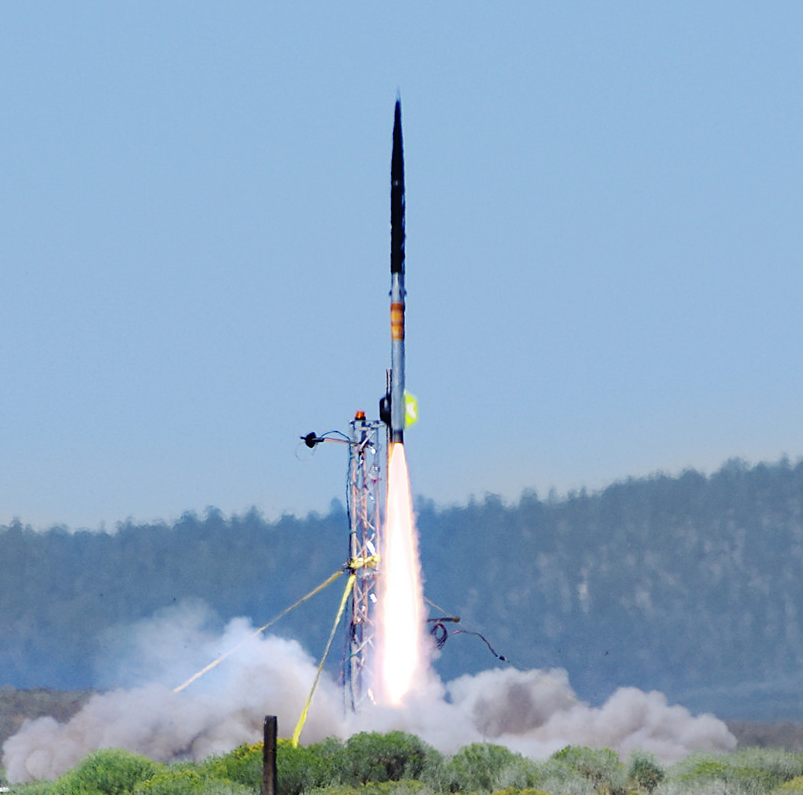
\includegraphics[width=\linewidth]{../img/L12-cropped.png}
\caption{PSAS' LV2 rocket lifting off for the group's $13^\text{th}$launch. The custom cylindrical patch antenna can be seen as a brown band around the middle of the rocket.}
\label{fig:L-12}
\end{wrapfigure}

The Portland State Aerospace Society (PSAS) is an interdisciplinary group of engineering students and alumni of Portland State University (PSU) with the long term goal of putting a cubesat into orbit with their own rocket. 
% info about cubesat market growth: http://www.spaceref.com/news/viewpr.html?pid=44940 
Their current airframe, named Launch Vehicle 2 (LV2), has served for over 12 years, representing 10 of the group's 13 launches, and hosted experiments ranging from custom patch antennas and long range WiFi technology to GPS navigation and a cold gas reaction control system (figure \ref{fig:L-12}). The LV2 platform is mostly constructed of aluminum with a fiberglass shell, with many of the parts having been fabricated in home garages. This makes for a robust but heavy design. Additionally, this airframe is built with a 4.5 inch inner diameter which PSAS's experiments have outgrown. 

The new airframe being designed, named Launch Vehicle 3 (LV3), aims to address these issues. The LV3 platform uses a 6 inch inner diameter, modules composed of carbon fiber and thin aluminum coupling rings, a carbon fiber nose cone, and a carbon fiber fin section. All of the airframe components connect via standardized rings, to accommodate future experimental modules and flight configurations.
The cylindrical LV3 airframe modules outperform the old design with an \weightReduction{} reduction in weight.
% Do we know what the increase in strength is? Also, can we confirm the weight reduction?

\subsection{Basic Design}

The majority of the LV3 airframe uses a sandwich shell composed of CF faces surrounding an aramid honeycomb core (see figure \ref{fig:moduleDiagram}). This provides a rigid structure while minimizing weight. 
Single sheets of carbon fiber are rigid when subjected to in-plane loading, and very flexible in bending. Meanwhile, the core is flexible in bending, and rigid under out-of-plane loading. 
When laminated together, these form a plate which is rigid in all loading conditions. The core material separates the rigid CF faces, greatly increasing the second moment of inertia of the plate. 
There is much more to the theory of sandwich plates and beams, but that is outside the scope of this paper. 

The body of the airframe is composed of modular cylindrical sections using this sandwich design with aluminum coupling rings co-molded to each end.
Each module can hold avionics, experiments, or other equipment with six tapped holes around the inside of the female coupling ring. 
For the radio module, FG takes the place of the CF to allow radio transparency.

The fins use the same sandwich design, with an aluminum frame defining their planform. The center of the frame is filled with core material, and the whole surface is covered in carbon fiber. 
The leading and trailing edges of the fins are made of machined phenolic resin, co-bonded with the frame and CF faces. 
The fins are fins are attached to a module with epoxy fillets, using chopped CF as a filler, and ``tip-to-tip'' CF sheets running from the tip of one fin across the module to the tip of the other fin.

The nose cone uses the same coupling ring system as the modules. It is a von K\'arm\'an ogive formed from two molded CF shells. 
Unlike the rest of the airframe, the nose cone uses a thin shell of two CF sheets, rather than a sandwich design (see section \ref{sec:noseCone} for details). 
The tip of the nose cone is machined out of aluminum and is removed when assembling the recovery system inside the nose cone. 

\begin{figure}
\centering
\def\svgwidth{\linewidth}
\parbox{0.45\linewidth}{
	\input{moduleDiagram.pdf_tex}
	\caption{
		Diagram of the male end of a module. 
		The CF (1) is bonded to the honeycomb core (3) and the aluminum coupling ring (4) using structural adhesive (2). 
		The adhesive also serves as a protective coating for the CF and provides a smooth outer surface. 
		See figure \ref{fig:coupon} for a picture of this design.
		}
	\label{fig:moduleDiagram}
}
\hfill
\parbox{0.45\linewidth}{
	\input{coupon.pdf_tex}
	\caption{
		A cut-away sample displaying the layers used in the LV3 sandwich shells. 
		See figure \ref{fig:moduleDiagram} for a diagramatic depiction.
		}
	\label{fig:coupon}
}
\end{figure}

\subsection{Significance}
Many amateur and university rocketry groups use composite airframes. However, these designs use many layers of fabric, with low fiber volume fractions.
While easy and durable, this does not fully take advantage of their materials. The LV3 design achieves a much higher specific strength and rigidity, enabling greater altitudes with a given motor. 

This design also occupies an uncommon regime for sandwich shell designs. Most such designs use sandwich shells in large, low curvature parts, whereas the LV3 modules have a relatively small size and high curvature.

This is also the only fully open-hardware rocket airframe in the HPR level 3 range. All of the documentation, design, and testing information if freely available on PSAS's Github page \cite{LV3repo}.
%----------need to make extra-sure there aren't any other open-hardware airframes out there----------

\subsection{Software}
\subsubsection{OpenRocket}
For the early design of amateur and university-scale rockets, \href{http://openrocket.sourceforge.net/}{OpenRocket} is very useful. 
It is an open-source Java application which simulates a rocket's flight. It provides a convenient interface for configuring the rocket, selecting commercial or custom parts, viewing the predictions, and performing some basic optimization. 

Using OpenRocket to guide the initial design allowed for rapid iteration of the fin geometry and the placement of non-airframe components. 

\subsubsection{OpenFOAM}
OpenFOAM is another open-source application. It provides a common interface for a wide range of CFD solvers.
Although it requires more up-front effort, it allows a more detailed perspective on what features of an airframe's geometry are the most critical. 
CFD analysis is probably not necessary for most amateur and university level airframe design, but this provides a good option for groups that can't afford a licence for a commercial CFD suite. 

OpenFoam was used to asses the heating at the tip of the nose, to determine if the epoxy matrix of the carbon fiber would degrade over repeated flights.


\section{Materials}
% Joe: I thought this section should talk about the materials that were donated i.e.: Meltbond 1515, Cytec Carbon Fiber, Non-silicone paste wax, etc and save the how we got it for the aquisition section. What do you think?
Nearly all of the materials used in the LV3 airframe were donated. The pre-impregnated CF and the structural adhesive were made available after they expired for use in commercial aircraft. 
Acquiring expired materials from large manufacturers and distributors is the strongly preferred over purchasing them outright or simply using cheaper materials. 
Distributors are unlikely to offer these materials in quantities appropriate to this type of project. 
Using carbon fiber cloth with painted-on epoxy could change the manufacturing significantly, and would increase the weight of the airframe. 
Acquiring donations is also a good way for university groups to form industry contacts. It can even become an opportunity to collaborate with other university groups, through the re-donation of excess material. 

The CF is a plain weave design that is pre-impregnated with epoxy resin which cures at $\SI{350}{\Far}$.
Meanwhile, the adhesive is an epoxy film which cures between $\SI{250}{\Far}$ and $\SI{350}{\Far}$, intended for bonding metals and composites. 
This allows for co-curing of both materials together. The core material is an over-expanded honeycomb Nomex$^\mathregistered$ mat which bonds well to the adhesive.
Finally, the coupling rings are machined out of 6061-T6 aluminum. 

Any groups obtaining materials through donations will likely not have much control over what materials they get, let alone be able to obtain the exact same materials listed here.
As such, any potential donations should be researched before they are accepted and tested afterwards. 
Any weave of CF will work, though satin is preferred. Pre-impregnated CF should be tacky at room temperature.
Adhesive should either be tacky at room temperature or become tacky when heated. Ideally, it should flow at higher temperatures. 
The core material for the modules should be over-expanded or under-expanded. 
Optimally expanded honeycomb cannot be used for the modules, since it ``potato chips'', bending away from the module along the axis when it is bent around the circumference. 
The fin core material may use any cell shape and should be $\nicefrac{1}{8}''$ or smaller. 
%---------check what the preferred notation is for length (fractional inches, decimal inches, centimeters...)---------

\subsection{Acquisition}
% Joe: I cannot think of anything else to add to this section after editing it. 
The open source nature of PSAS and the LV3 project meant that operations rely heavily on the donations of individuals in the community and local industry. Composite materials in the quantity needed to build a complete rocket required funding which was far outside of the means of the PSAS budget. Large composite manufacturers and aerospace companies were contacted about interest in donating expired materials or potential sponsorships. 

Strong industry relationships were built creating reliable sources for materials for the time being and into the future. A substantial source of the material donations made during the composite airframe project was made by Boeing. They supplied PSAS with two rolls of pre-impregnated carbon fiber, structural adhesive, vacuum bagging kits made up of hight temperature bagging material, release film, tape, and breather material. Additionally, Boeing also provided professional consulting with industry experts who made time available to us on a weekly basis. 

Boeing and Pacific Coast Composites donated several rolls of 250°F and 350°F pre-impregnated fiberglass of which Portland State could not supply appropriate storage for. Rolls were dispersed through the campus and local companies offered cold storage in trade for material. This prompted contacting other universities in the region to offer the excess materials as a donation to their clubs. PSAS donated tens of thousands of dollars in fiberglass to Oregon State University and Washington State University's aerospace and motor sports clubs. 

\section{Cylindrical Modules}\label{sec:modules}

\begin{figure}[t]
	\centering
	\parbox{0.45\linewidth}
	{
		\centering
		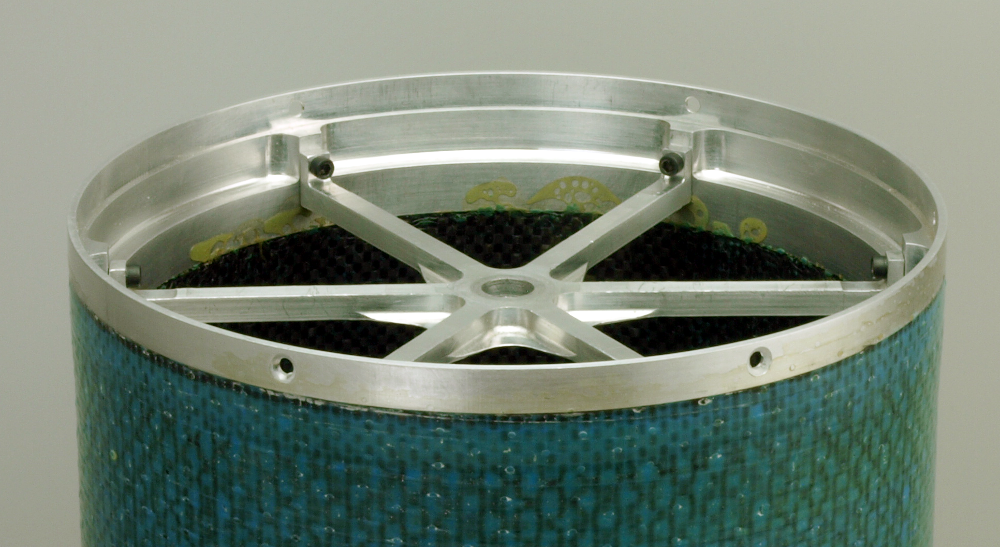
\includegraphics[width=\linewidth]{../img/moduleWithSpider.png}
		\caption{A CF module with the ``spider'' attachment, which retains the motor in the rocket. The female end is shown.}
		\label{fig:module}
	}
	\hfill
	\parbox{0.45\linewidth}
	{
		\centering
		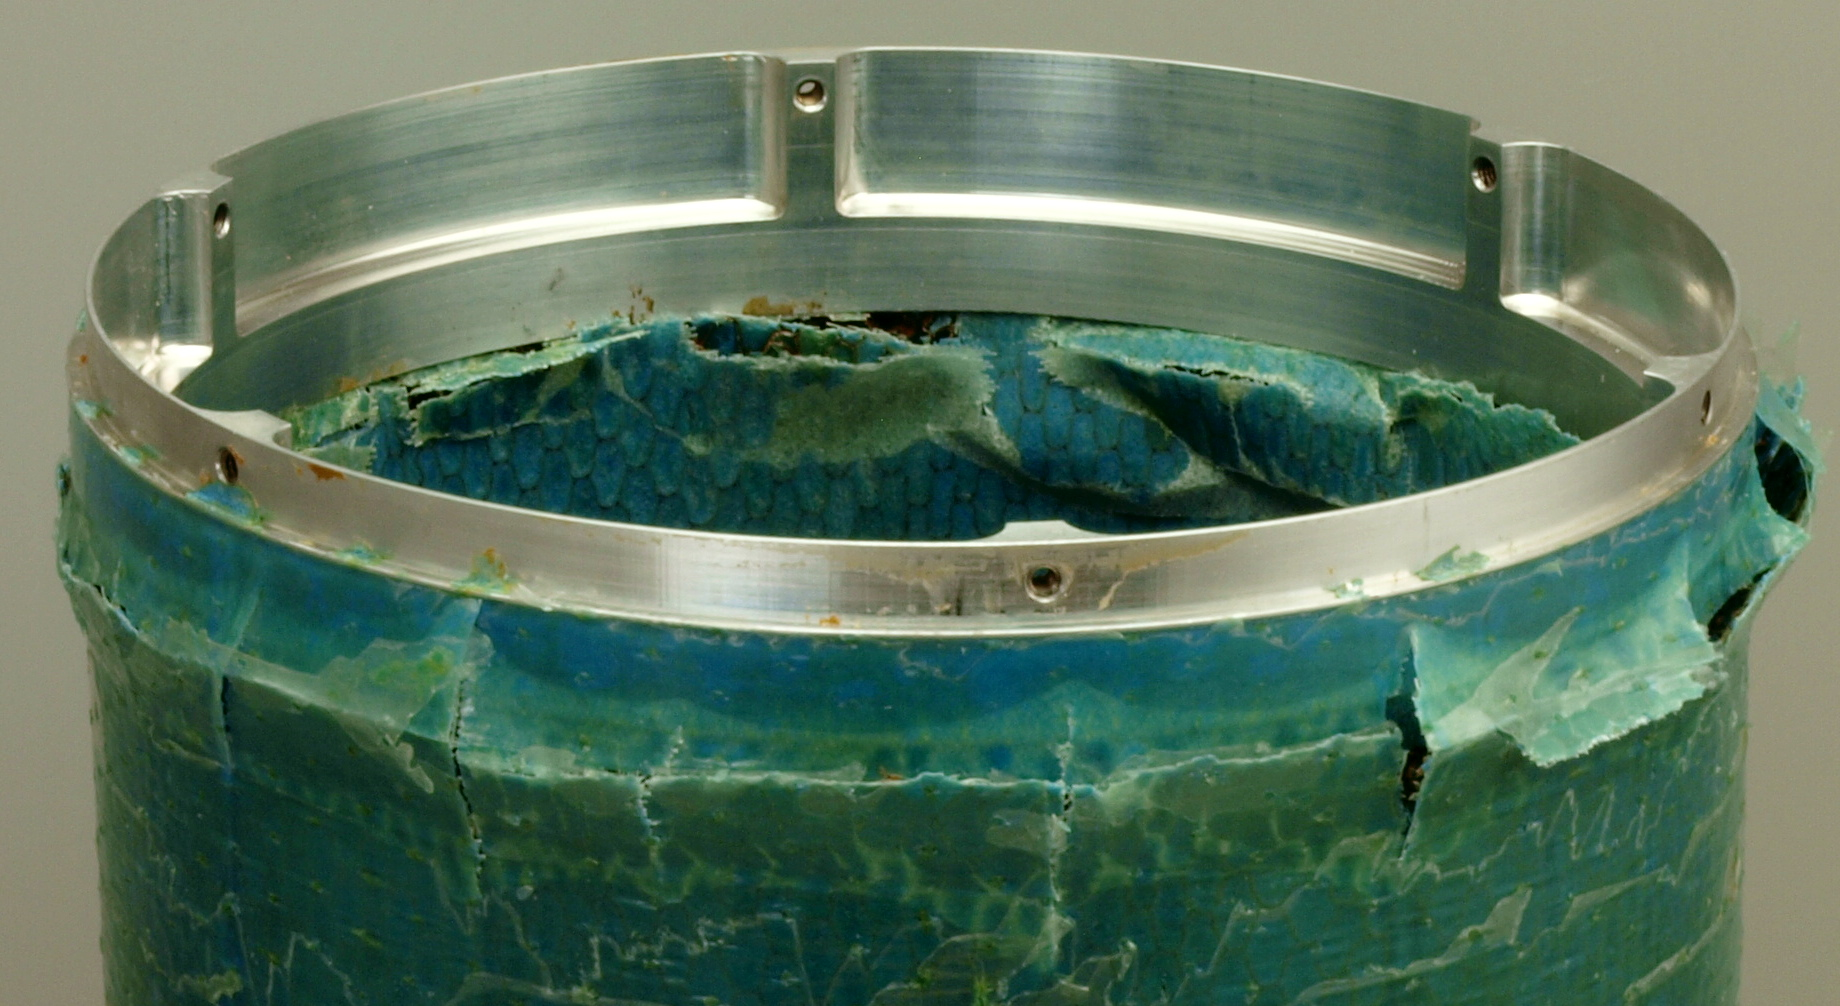
\includegraphics[width=\linewidth]{../img/FG_fracture.jpg}
		\caption{A fiberglass module after failing in compression. Note that the failure on the inner and outer layers occured at the same height. The male end is shown.}
		\label{fig:crush}
	}
\end{figure}

Each module has a male coupling ring on the end facing the direction of travel and a female coupling ring on the other end. 
Modules were made in both $18''$ and $24''$ lengths, to accommodate different lengths of motors and equipment. 
By exchanging modules of different lengths, this also allows the overall length of the rocket to be adjusted in increments of $6''$.
The body of the module consists of two concentric CF tubes separated by a honeycomb core, with adhesive bonding the CF to the core and rings (see figure \ref{fig:moduleDiagram}). 
A layer of adhesive also covers the outer layer of CF, serving three roles. First, it ensures the outer layer of CF is completely wetted. 
The pre-impregnated CF used here did not completely wet when cured alone, however this will not be true for every product.
Second, it serves as a protective coating for the CF. 
Third, it can be sanded to improve the surface roughness.
Using a profilometer, the surface features of the uncoated modules was found to be $\SI{179}{\micro\meter}$ ($\SI{7.1e-3}{in}$), while the surface features of the adhesive-coated modules could be sanded to $\SI{3.3}{\micro\meter}$ ($\SI{1.3e-4}{in}$).

\begin{figure}[t]
	\centering
	\parbox{0.45\linewidth}
	{
		\centering
		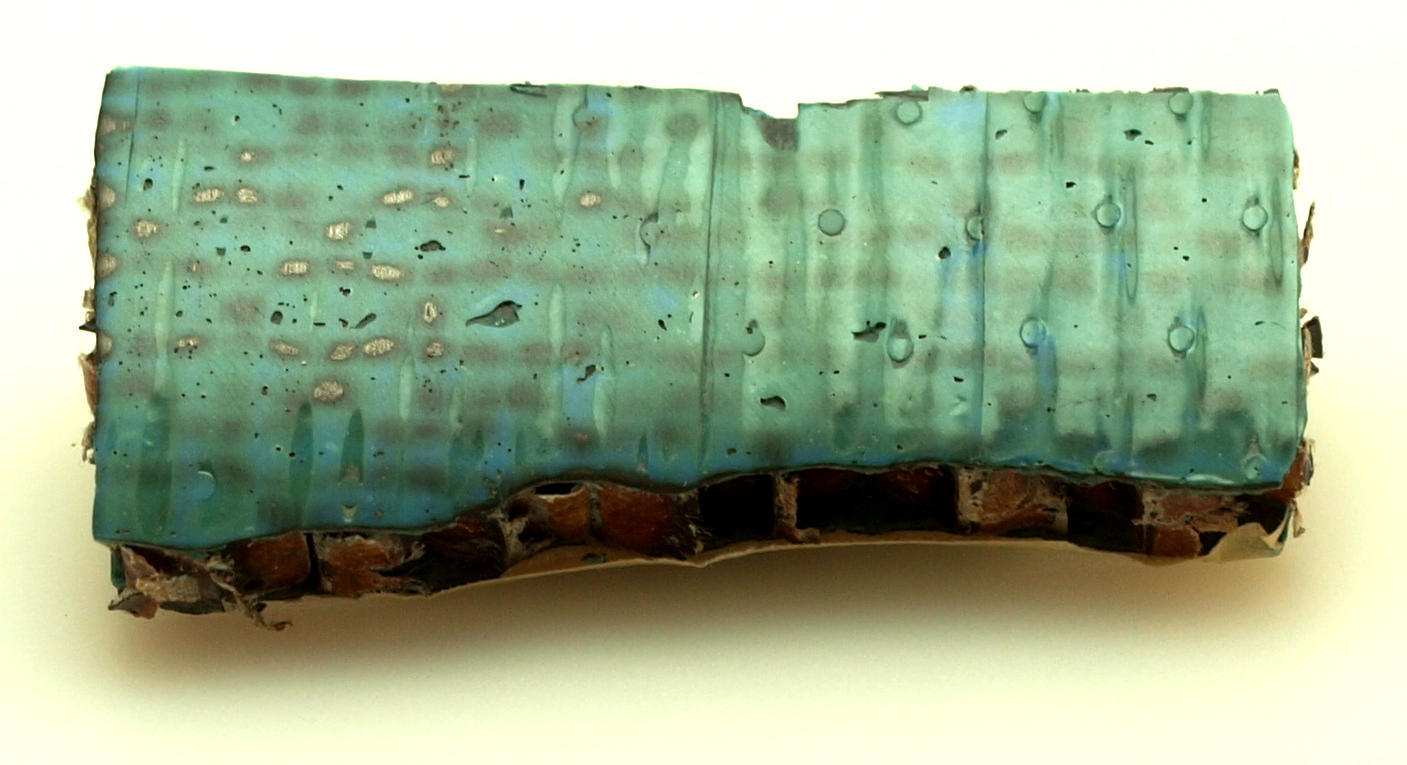
\includegraphics[width=\linewidth]{../img/coated.JPG}	
		\caption{A sandwich plate sample which has been coated with structural adhesive. The left side has been sanded and polished. See figure \ref{fig:roughness} for a plot of the surface profile.}
		\label{fig:coated}
	}
	\hfill
	\parbox{0.45\linewidth}
	{
		\centering
		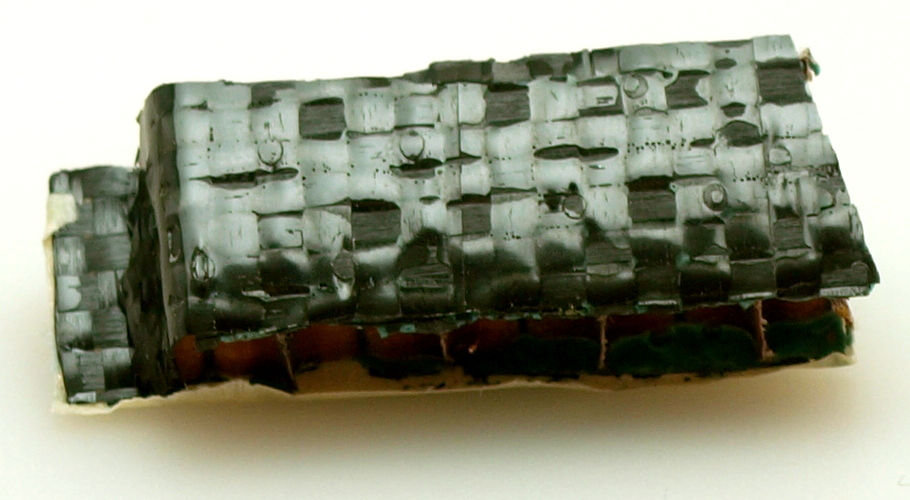
\includegraphics[width=\linewidth]{../img/uncoated.JPG}	
		\caption{A sandwich plate sample which has \emph{not} been coated with structural adhesive. See figure \ref{fig:roughness} for a plot of the surface profile. Note the dry cells where the epoxy has not wetted the CF.}
		\label{fig:uncoated}
	}
	\parbox{4in}
	{
		\centering
		% Created by tikzDevice version 0.10.1 on 2016-08-17 11:40:13
% !TEX encoding = UTF-8 Unicode
\begin{tikzpicture}[x=1pt,y=1pt]
\definecolor{fillColor}{RGB}{255,255,255}
\path[use as bounding box,fill=fillColor,fill opacity=0.00] (0,0) rectangle (289.08,216.81);
\begin{scope}
\path[clip] ( 48.00, 48.00) rectangle (289.08,204.81);
\definecolor{drawColor}{RGB}{0,0,0}

\path[draw=drawColor,line width= 0.4pt,line join=round,line cap=round] ( 56.93, 63.08) --
	( 57.15, 62.62) --
	( 57.60, 62.31) --
	( 57.94, 61.85) --
	( 58.39, 61.22) --
	( 58.84, 60.61) --
	( 59.18, 60.14) --
	( 59.62, 60.30) --
	( 59.96, 60.46) --
	( 60.40, 60.62) --
	( 60.84, 60.93) --
	( 61.18, 61.24) --
	( 61.62, 61.40) --
	( 62.07, 61.72) --
	( 62.40, 62.03) --
	( 62.84, 62.03) --
	( 63.18, 62.03) --
	( 63.62, 62.04) --
	( 64.07, 61.73) --
	( 64.41, 61.42) --
	( 64.52, 61.26) --
	( 64.64, 60.80) --
	( 64.75, 60.18) --
	( 64.75, 59.55) --
	( 64.87, 59.09) --
	( 64.87, 58.46) --
	( 64.88, 57.84) --
	( 64.88, 57.37) --
	( 65.11, 56.75) --
	( 65.22, 56.44) --
	( 65.33, 55.82) --
	( 65.56, 55.20) --
	( 65.79, 54.73) --
	( 66.24, 54.43) --
	( 66.57, 54.12) --
	( 67.02, 53.81) --
	( 67.46, 54.28) --
	( 67.68, 54.59) --
	( 68.02, 55.06) --
	( 68.46, 55.53) --
	( 68.68, 55.84) --
	( 69.01, 56.31) --
	( 69.34, 56.78) --
	( 69.79, 57.10) --
	( 70.01, 57.56) --
	( 70.34, 58.03) --
	( 70.56, 58.50) --
	( 70.89, 58.97) --
	( 71.11, 59.44) --
	( 71.44, 59.91) --
	( 71.66, 60.38) --
	( 71.88, 61.00) --
	( 71.99, 61.62) --
	( 72.21, 62.09) --
	( 72.32, 62.72) --
	( 72.43, 63.18) --
	( 72.64, 63.81) --
	( 72.86, 64.43) --
	( 72.97, 64.90) --
	( 73.19, 65.37) --
	( 73.30, 65.84) --
	( 73.52, 66.15) --
	( 73.75, 65.53) --
	( 73.86, 65.22) --
	( 73.98, 64.60) --
	( 74.20, 63.97) --
	( 74.32, 63.51) --
	( 74.43, 62.89) --
	( 74.66, 62.42) --
	( 74.77, 61.80) --
	( 74.89, 61.18) --
	( 75.00, 60.71) --
	( 75.23, 60.24) --
	( 75.35, 59.62) --
	( 75.46, 59.16) --
	( 75.57, 58.69) --
	( 75.91, 58.54) --
	( 76.36, 58.38) --
	( 76.80, 58.07) --
	( 77.14, 57.92) --
	( 77.59, 57.77) --
	( 77.92, 57.46) --
	( 78.37, 57.62) --
	( 78.81, 58.09) --
	( 78.92, 57.78) --
	( 78.70, 57.78) --
	( 78.48, 57.93) --
	( 78.81, 57.78) --
	( 79.04, 57.78) --
	( 79.14, 58.25) --
	( 79.25, 58.87) --
	( 79.36, 59.49) --
	( 79.36, 59.96) --
	( 79.58, 60.58) --
	( 79.57, 61.05) --
	( 79.79, 61.68) --
	( 79.90, 62.30) --
	( 80.01, 62.77) --
	( 80.34, 63.24) --
	( 80.56, 63.86) --
	( 80.89, 64.17) --
	( 81.11, 64.64) --
	( 81.33, 64.95) --
	( 81.55, 65.58) --
	( 81.77, 66.05) --
	( 82.10, 66.52) --
	( 82.43, 67.14) --
	( 82.65, 67.61) --
	( 83.10, 68.08) --
	( 83.54, 68.24) --
	( 83.77, 68.40) --
	( 83.99, 68.71) --
	( 84.32, 69.02) --
	( 84.43, 69.49) --
	( 84.76, 69.96) --
	( 84.98, 70.43) --
	( 85.31, 70.90) --
	( 85.64, 71.21) --
	( 85.97, 71.68) --
	( 86.31, 72.15) --
	( 86.53, 72.46) --
	( 86.97, 72.93) --
	( 87.42, 72.78) --
	( 87.75, 72.78) --
	( 88.20, 72.63) --
	( 88.53, 72.78) --
	( 88.64, 73.25) --
	( 88.64, 73.88) --
	( 88.75, 74.34) --
	( 88.74, 74.97) --
	( 88.85, 75.59) --
	( 88.85, 76.06) --
	( 88.95, 76.68) --
	( 88.95, 77.30) --
	( 89.06, 77.77) --
	( 89.06, 78.39) --
	( 89.16, 78.86) --
	( 89.16, 79.48) --
	( 89.27, 80.11) --
	( 89.38, 80.57) --
	( 89.37, 81.20) --
	( 89.48, 81.67) --
	( 89.48, 82.29) --
	( 89.59, 82.91) --
	( 89.69, 83.38) --
	( 89.80, 84.00) --
	( 89.91, 84.47) --
	( 89.91, 84.94) --
	( 89.90, 85.56) --
	( 89.90, 86.03) --
	( 89.90, 86.65) --
	( 90.01, 87.12) --
	( 90.00, 87.58) --
	( 90.11, 88.21) --
	( 90.22, 88.68) --
	( 90.33, 89.30) --
	( 90.43, 89.92) --
	( 90.54, 90.39) --
	( 90.76, 91.01) --
	( 90.98, 91.48) --
	( 91.20, 91.95) --
	( 91.42, 92.58) --
	( 91.64, 92.89) --
	( 91.97, 93.51) --
	( 92.19, 94.14) --
	( 92.41, 94.45) --
	( 92.75, 94.76) --
	( 92.86, 94.30) --
	( 93.09, 93.68) --
	( 93.31, 93.05) --
	( 93.43, 92.59) --
	( 93.54, 91.97) --
	( 93.77, 91.35) --
	( 93.88, 91.03) --
	( 93.89, 90.41) --
	( 93.89, 89.94) --
	( 93.89, 89.32) --
	( 93.90, 88.70) --
	( 93.90, 88.23) --
	( 94.02, 87.61) --
	( 94.13, 87.14) --
	( 94.25, 86.52) --
	( 94.36, 85.90) --
	( 94.48, 85.43) --
	( 94.59, 84.81) --
	( 94.93, 84.19) --
	( 95.26, 84.19) --
	( 95.71, 84.20) --
	( 96.04, 84.20) --
	( 96.49, 84.20) --
	( 96.82, 84.05) --
	( 96.71, 84.36) --
	( 97.04, 84.83) --
	( 97.15, 85.45) --
	( 97.37, 85.76) --
	( 97.48, 86.39) --
	( 97.59, 86.85) --
	( 97.81, 87.48) --
	( 98.03, 88.10) --
	( 98.14, 88.57) --
	( 98.35, 89.20) --
	( 98.46, 89.66) --
	( 98.68, 90.29) --
	( 98.79, 90.91) --
	( 98.90, 91.22) --
	( 99.12, 91.85) --
	( 99.23, 92.47) --
	( 99.45, 92.94) --
	( 99.67, 93.56) --
	( 99.89, 93.56) --
	(100.00, 94.03) --
	(100.22, 93.57) --
	(100.23, 93.10) --
	(100.34, 92.48) --
	(100.46, 92.01) --
	(100.46, 91.39) --
	(100.57, 90.77) --
	(100.69, 90.30) --
	(100.80, 89.68) --
	(100.92, 89.06) --
	(100.92, 88.59) --
	(101.04, 87.97) --
	(101.15, 87.50) --
	(101.16, 86.88) --
	(101.27, 86.26) --
	(101.39, 85.79) --
	(101.50, 85.17) --
	(101.61, 84.86) --
	(102.06, 84.70) --
	(102.51, 84.40) --
	(102.73, 84.71) --
	(103.06, 85.33) --
	(103.28, 85.80) --
	(103.39, 86.27) --
	(103.72, 86.89) --
	(103.83, 87.36) --
	(104.05, 87.83) --
	(104.27, 88.45) --
	(104.49, 88.92) --
	(104.82, 89.55) --
	(105.04, 90.02) --
	(105.26, 90.64) --
	(105.59, 91.27) --
	(105.81, 91.73) --
	(106.03, 92.20) --
	(106.25, 92.20) --
	(106.37, 91.74) --
	(106.48, 91.12) --
	(106.60, 90.65) --
	(106.82, 90.03) --
	(106.94, 89.41) --
	(107.05, 88.94) --
	(107.28, 88.32) --
	(107.39, 87.70) --
	(107.51, 87.23) --
	(107.74, 86.61) --
	(107.85, 86.14) --
	(107.96, 85.52) --
	(108.30, 85.52) --
	(108.41, 85.99) --
	(108.52, 86.61) --
	(108.74, 86.93) --
	(108.84, 87.55) --
	(108.95, 88.17) --
	(109.06, 88.64) --
	(109.28, 89.27) --
	(109.50, 89.89) --
	(109.61, 90.36) --
	(109.72, 90.98) --
	(109.94, 91.45) --
	(110.04, 92.07) --
	(110.15, 92.70) --
	(110.26, 93.16) --
	(110.48, 93.79) --
	(110.59, 94.26) --
	(110.81, 94.88) --
	(110.91, 95.50) --
	(111.02, 95.82) --
	(111.24, 96.44) --
	(111.58, 96.60) --
	(111.91, 96.44) --
	(112.36, 96.29) --
	(112.69, 96.29) --
	(113.14, 96.14) --
	(113.37, 95.68) --
	(113.37, 95.21) --
	(113.48, 94.59) --
	(113.60, 94.12) --
	(113.71, 93.50) --
	(113.83, 92.88) --
	(113.94, 92.41) --
	(114.06, 91.79) --
	(114.17, 91.17) --
	(114.18, 90.70) --
	(114.29, 90.08) --
	(114.41, 89.61) --
	(114.52, 88.99) --
	(114.64, 88.37) --
	(114.75, 88.06) --
	(114.86, 88.68) --
	(114.97, 89.15) --
	(115.07, 89.77) --
	(115.18, 90.39) --
	(115.29, 90.86) --
	(115.40, 91.48) --
	(115.51, 92.11) --
	(115.50, 92.58) --
	(115.61, 93.20) --
	(115.72, 93.67) --
	(115.83, 94.29) --
	(115.93, 94.91) --
	(116.04, 95.38) --
	(116.15, 96.00) --
	(116.49, 95.54) --
	(116.71, 95.23) --
	(116.94, 94.76) --
	(117.16, 94.30) --
	(117.50, 93.83) --
	(117.73, 93.37) --
	(117.95, 93.06) --
	(118.29, 92.59) --
	(118.51, 92.28) --
	(118.85, 91.66) --
	(119.19, 91.04) --
	(119.42, 90.73) --
	(119.75, 90.27) --
	(120.09, 90.27) --
	(120.42, 90.27) --
	(120.75, 90.59) --
	(120.97, 91.05) --
	(121.20, 91.52) --
	(121.42, 91.99) --
	(121.64, 92.46) --
	(121.97, 93.08) --
	(122.19, 93.55) --
	(122.52, 94.18) --
	(122.96, 94.18) --
	(123.19, 93.71) --
	(123.53, 93.25) --
	(123.86, 92.79) --
	(124.09, 92.32) --
	(124.20, 91.70) --
	(124.21, 91.23) --
	(124.32, 90.61) --
	(124.55, 90.14) --
	(124.55, 89.68) --
	(124.55, 89.05) --
	(124.45, 88.59) --
	(124.56, 88.43) --
	(124.78, 89.05) --
	(124.89, 89.52) --
	(124.88, 89.83) --
	(124.77, 89.52) --
	(124.55, 89.21) --
	(124.56, 88.59) --
	(124.78, 88.90) --
	(125.11, 89.52) --
	(125.33, 90.15) --
	(125.55, 90.62) --
	(125.77, 91.08) --
	(125.88, 91.55) --
	(126.21, 92.18) --
	(126.43, 92.80) --
	(126.65, 93.27) --
	(126.87, 93.89) --
	(127.09, 94.36) --
	(127.20, 94.83) --
	(127.42, 95.30) --
	(127.64, 95.77) --
	(127.85, 96.39) --
	(127.97, 96.24) --
	(128.08, 96.08) --
	(128.19, 95.46) --
	(128.31, 94.99) --
	(128.42, 94.37) --
	(128.54, 93.91) --
	(128.65, 93.44) --
	(128.77, 92.82) --
	(128.88, 92.19) --
	(129.00, 91.73) --
	(129.11, 91.11) --
	(129.23, 90.64) --
	(129.45, 90.02) --
	(129.57, 89.40) --
	(129.68, 88.93) --
	(129.80, 88.31) --
	(129.91, 88.62) --
	(129.91, 89.09) --
	(130.01, 89.71) --
	(130.12, 90.18) --
	(130.45, 90.49) --
	(130.79, 90.96) --
	(131.01, 91.43) --
	(131.34, 91.90) --
	(131.56, 92.21) --
	(131.78, 92.68) --
	(132.11, 93.15) --
	(132.33, 93.62) --
	(132.66, 94.24) --
	(132.88, 94.71) --
	(133.10, 95.02) --
	(133.43, 95.65) --
	(133.65, 95.96) --
	(133.99, 96.43) --
	(134.32, 97.06) --
	(134.54, 97.37) --
	(134.76, 97.99) --
	(134.98, 98.31) --
	(135.31, 98.77) --
	(135.53, 99.24) --
	(135.86, 99.71) --
	(135.97,100.18) --
	(136.08, 99.87) --
	(136.20, 99.40) --
	(136.42, 98.78) --
	(136.54, 98.47) --
	(136.76, 97.85) --
	(136.88, 97.23) --
	(137.10, 96.92) --
	(137.22, 96.30) --
	(137.45, 95.83) --
	(137.67, 95.21) --
	(137.79, 94.59) --
	(138.01, 94.12) --
	(138.24, 93.50) --
	(138.36, 92.88) --
	(138.58, 92.41) --
	(138.81, 91.79) --
	(138.92, 91.33) --
	(139.15, 90.70) --
	(139.38, 90.08) --
	(139.60, 89.77) --
	(139.60, 89.31) --
	(139.61, 88.84) --
	(139.61, 88.22) --
	(139.72, 88.06) --
	(139.83, 88.53) --
	(139.83, 89.15) --
	(139.94, 89.78) --
	(139.93, 90.24) --
	(140.04, 90.87) --
	(140.15, 91.33) --
	(140.37, 91.80) --
	(140.48, 92.43) --
	(140.70, 92.89) --
	(140.80, 93.52) --
	(141.02, 93.99) --
	(141.13, 94.45) --
	(141.24, 95.08) --
	(141.35, 95.54) --
	(141.57, 96.17) --
	(141.79, 96.79) --
	(141.90, 97.26) --
	(142.12, 97.89) --
	(142.22, 98.35) --
	(142.33, 98.98) --
	(142.55, 99.44) --
	(142.89, 99.60) --
	(143.33, 99.61) --
	(143.67, 99.76) --
	(144.00, 99.76) --
	(144.23, 99.30) --
	(144.34, 98.83) --
	(144.57, 98.21) --
	(144.68, 97.59) --
	(144.91, 97.12) --
	(145.02, 96.50) --
	(145.14, 96.04) --
	(145.36, 95.41) --
	(145.48, 94.79) --
	(145.71, 94.33) --
	(145.82, 93.71) --
	(146.05, 93.08) --
	(146.16, 92.62) --
	(146.28, 92.15) --
	(146.50, 91.69) --
	(146.39, 91.06) --
	(146.40, 90.44) --
	(146.51, 90.44) --
	(146.39, 91.06) --
	(146.39, 91.53) --
	(146.51, 90.91) --
	(146.29, 90.59) --
	(146.29, 90.13) --
	(146.29, 89.50) --
	(146.30, 88.88) --
	(146.30, 88.73) --
	(146.40, 89.35) --
	(146.51, 89.82) --
	(146.62, 90.44) --
	(146.73, 91.06) --
	(146.84, 91.53) --
	(147.06, 92.00) --
	(147.17, 92.31) --
	(147.50, 92.94) --
	(147.83, 93.56) --
	(148.05, 94.03) --
	(148.27, 94.50) --
	(148.60, 94.97) --
	(148.82, 95.13) --
	(149.27, 95.13) --
	(149.60, 95.13) --
	(150.05, 94.98) --
	(150.50, 94.98) --
	(150.83, 94.98) --
	(151.28, 94.83) --
	(151.72, 94.68) --
	(151.73, 94.21) --
	(151.84, 93.59) --
	(151.84, 93.12) --
	(151.96, 92.50) --
	(152.08, 91.88) --
	(152.08, 91.41) --
	(152.19, 90.79) --
	(152.20, 90.32) --
	(152.31, 89.70) --
	(152.32, 89.08) --
	(152.43, 88.61) --
	(152.43, 87.99) --
	(152.55, 87.37) --
	(152.55, 86.90) --
	(152.67, 86.28) --
	(152.67, 85.81) --
	(152.79, 85.19) --
	(152.90, 84.57) --
	(152.90, 84.10) --
	(153.02, 83.48) --
	(153.02, 83.01) --
	(153.14, 82.39) --
	(153.14, 81.76) --
	(153.25, 81.30) --
	(153.26, 80.68) --
	(153.37, 80.05) --
	(153.38, 79.59) --
	(153.49, 78.96) --
	(153.49, 78.50) --
	(153.61, 77.88) --
	(153.61, 77.25) --
	(153.73, 76.79) --
	(153.84, 76.16) --
	(153.85, 75.70) --
	(153.95, 76.32) --
	(153.95, 76.63) --
	(153.96, 76.17) --
	(154.07, 75.70) --
	(154.07, 75.39) --
	(154.18, 75.86) --
	(154.18, 76.48) --
	(154.28, 76.95) --
	(154.62, 77.10) --
	(154.84, 77.57) --
	(155.06, 78.04) --
	(155.05, 78.66) --
	(155.05, 79.13) --
	(155.27, 79.75) --
	(155.49, 80.38) --
	(155.71, 80.85) --
	(155.82, 81.47) --
	(156.04, 82.09) --
	(156.26, 82.56) --
	(156.25, 83.19) --
	(156.36, 83.65) --
	(156.47, 84.28) --
	(156.69, 84.90) --
	(156.80, 85.37) --
	(156.91, 85.99) --
	(157.13, 86.46) --
	(157.23, 86.93) --
	(157.45, 87.55) --
	(157.56, 87.87) --
	(157.78, 88.49) --
	(157.89, 89.11) --
	(158.00, 89.58) --
	(157.99, 90.20) --
	(158.10, 90.67) --
	(158.55, 91.14) --
	(158.54, 91.76) --
	(158.76, 92.23) --
	(158.87, 92.70) --
	(159.09, 93.32) --
	(159.09, 93.79) --
	(159.19, 94.41) --
	(159.30, 94.88) --
	(159.52, 95.51) --
	(159.74, 96.13) --
	(159.85, 96.60) --
	(159.96, 97.22) --
	(160.07, 97.69) --
	(160.18, 98.16) --
	(160.28, 98.78) --
	(160.50, 99.25) --
	(160.72, 99.87) --
	(160.94,100.50) --
	(161.05,100.97) --
	(161.38,101.59) --
	(161.38,102.06) --
	(161.60,102.68) --
	(161.82,103.31) --
	(162.04,103.77) --
	(162.26,104.40) --
	(162.36,104.87) --
	(162.69,105.49) --
	(162.91,106.12) --
	(163.13,106.58) --
	(163.24,107.21) --
	(163.57,107.83) --
	(163.68,108.30) --
	(163.79,108.92) --
	(163.90,109.39) --
	(164.23,110.02) --
	(164.34,110.64) --
	(164.56,111.11) --
	(164.66,111.73) --
	(164.88,112.20) --
	(165.10,112.82) --
	(165.32,113.29) --
	(165.32,113.76) --
	(165.65,114.38) --
	(165.87,115.01) --
	(165.98,115.48) --
	(166.20,116.10) --
	(166.42,116.57) --
	(166.53,117.19) --
	(166.74,117.82) --
	(166.85,118.28) --
	(167.07,118.75) --
	(167.29,119.38) --
	(167.40,119.69) --
	(167.62,120.31) --
	(167.62,120.78) --
	(167.84,121.40) --
	(168.06,122.03) --
	(168.17,122.50) --
	(168.27,123.12) --
	(168.38,123.59) --
	(168.49,124.21) --
	(168.71,124.68) --
	(168.82,125.15) --
	(168.93,125.77) --
	(169.14,126.39) --
	(169.25,126.86) --
	(169.25,127.48) --
	(169.36,127.95) --
	(169.58,128.58) --
	(169.69,129.04) --
	(169.91,129.51) --
	(170.01,130.14) --
	(170.23,130.45) --
	(170.34,131.07) --
	(170.56,131.70) --
	(170.67,132.01) --
	(170.89,132.63) --
	(171.00,133.26) --
	(171.11,133.72) --
	(171.33,134.35) --
	(171.43,134.82) --
	(171.54,135.44) --
	(171.65,136.06) --
	(171.87,136.53) --
	(172.09,137.16) --
	(172.20,137.62) --
	(172.42,138.09) --
	(172.64,138.72) --
	(172.75,139.18) --
	(172.85,139.81) --
	(173.07,140.28) --
	(173.18,140.74) --
	(173.40,141.37) --
	(173.51,141.68) --
	(173.73,142.30) --
	(173.84,142.93) --
	(174.06,143.40) --
	(174.28,144.02) --
	(174.39,144.49) --
	(174.61,144.96) --
	(174.82,145.58) --
	(174.93,145.89) --
	(175.15,146.36) --
	(175.60,146.99) --
	(175.70,147.45) --
	(175.93,147.92) --
	(176.15,148.23) --
	(176.37,148.86) --
	(176.58,149.48) --
	(176.80,149.95) --
	(176.91,150.58) --
	(177.13,151.04) --
	(177.46,151.67) --
	(177.79,152.29) --
	(177.90,152.76) --
	(178.12,153.23) --
	(178.45,153.70) --
	(178.56,154.17) --
	(178.78,154.79) --
	(178.89,155.26) --
	(179.22,155.73) --
	(179.44,156.20) --
	(179.66,156.66) --
	(179.88,157.29) --
	(180.21,157.76) --
	(180.43,158.23) --
	(180.65,158.85) --
	(180.87,159.16) --
	(181.20,159.79) --
	(181.54,160.10) --
	(181.65,160.57) --
	(181.98,161.04) --
	(182.09,161.51) --
	(182.19,162.13) --
	(182.41,162.60) --
	(182.63,163.07) --
	(182.85,163.69) --
	(183.18,164.32) --
	(183.52,164.47) --
	(183.96,164.48) --
	(184.30,164.48) --
	(184.74,164.48) --
	(185.19,164.49) --
	(185.52,164.49) --
	(185.97,164.49) --
	(186.30,164.49) --
	(186.75,164.03) --
	(187.09,163.72) --
	(187.43,163.25) --
	(187.87,162.95) --
	(188.32,162.48) --
	(188.55,162.33) --
	(188.88,161.86) --
	(189.22,161.71) --
	(189.55,161.56) --
	(189.77,162.02) --
	(189.99,162.49) --
	(190.33,162.96) --
	(190.44,163.27) --
	(190.77,163.74) --
	(190.99,164.37) --
	(191.21,164.83) --
	(191.20,165.46) --
	(191.20,166.08) --
	(191.20,166.55) --
	(191.30,167.17) --
	(191.41,167.64) --
	(191.63,168.26) --
	(191.63,168.89) --
	(191.63,169.36) --
	(191.62,169.97) --
	(191.73,170.44) --
	(191.84,171.06) --
	(191.95,171.69) --
	(191.94,172.16) --
	(192.05,172.78) --
	(192.16,173.25) --
	(192.16,173.71) --
	(192.15,174.33) --
	(192.26,174.80) --
	(192.37,175.43) --
	(192.59,176.05) --
	(192.70,176.52) --
	(192.80,176.99) --
	(192.91,177.61) --
	(193.02,178.08) --
	(193.13,178.71) --
	(193.24,179.17) --
	(193.35,179.79) --
	(193.57,180.26) --
	(193.67,180.73) --
	(193.89,181.35) --
	(194.00,181.82) --
	(194.22,182.45) --
	(194.33,183.07) --
	(194.55,183.54) --
	(194.77,184.16) --
	(194.88,184.79) --
	(194.98,185.26) --
	(195.20,185.73) --
	(195.31,186.19) --
	(195.53,186.82) --
	(195.64,187.44) --
	(195.86,187.90) --
	(195.86,188.53) --
	(195.85,189.00) --
	(195.85,189.62) --
	(195.85,190.24) --
	(196.07,190.71) --
	(196.28,191.34) --
	(196.50,191.96) --
	(196.72,192.27) --
	(196.94,192.90) --
	(197.16,193.37) --
	(197.38,193.83) --
	(197.72,194.14) --
	(198.05,194.14) --
	(198.50,194.15) --
	(198.83,194.15) --
	(199.28,194.31) --
	(199.72,194.78) --
	(200.05,194.94) --
	(200.39,195.10) --
	(200.83,195.10) --
	(201.17,195.10) --
	(201.61,195.11) --
	(201.95,195.11) --
	(202.39,195.11) --
	(202.84,195.12) --
	(203.17,195.12) --
	(203.62,195.27) --
	(203.95,195.43) --
	(204.40,195.59) --
	(204.84,195.75) --
	(205.18,195.91) --
	(205.62,196.06) --
	(206.07,196.23) --
	(206.40,196.23) --
	(206.85,196.23) --
	(207.18,196.07) --
	(207.63,196.08) --
	(208.07,196.23) --
	(208.41,196.40) --
	(208.85,196.55) --
	(209.29,196.86) --
	(209.63,196.87) --
	(210.07,197.18) --
	(210.41,197.19) --
	(210.85,197.19) --
	(211.30,197.19) --
	(211.64,197.03) --
	(212.08,197.04) --
	(212.42,197.04) --
	(212.86,197.21) --
	(213.31,197.36) --
	(213.64,197.52) --
	(214.08,197.83) --
	(214.53,197.99) --
	(214.86,198.15) --
	(215.31,198.15) --
	(215.64,198.15) --
	(216.09,198.16) --
	(216.53,198.16) --
	(216.87,198.16) --
	(217.32,198.01) --
	(217.65,198.01) --
	(218.10,198.01) --
	(218.54,198.01) --
	(218.88,198.02) --
	(219.32,198.02) --
	(219.77,198.02) --
	(220.10,198.02) --
	(220.55,198.18) --
	(220.88,198.18) --
	(221.33,198.35) --
	(221.77,198.51) --
	(222.11,198.66) --
	(222.55,198.98) --
	(222.88,198.98) --
	(223.33,198.98) --
	(223.78,198.99) --
	(224.11,198.99) --
	(224.56,198.99) --
	(225.00,198.99) --
	(225.34,198.99) --
	(225.78,198.99) --
	(226.12,199.00) --
	(226.56,199.00) --
	(227.01,198.85) --
	(227.34,198.85) --
	(227.79,198.86) --
	(228.12,198.86) --
	(228.57,198.86) --
	(229.02,198.86) --
	(229.35,198.86) --
	(229.80,198.86) --
	(230.24,198.87) --
	(230.58,198.72) --
	(231.02,198.72) --
	(231.36,198.72) --
	(231.80,198.73) --
	(232.25,198.73) --
	(232.58,198.73) --
	(233.03,198.74) --
	(233.48,198.74) --
	(233.81,198.74) --
	(234.26,198.74) --
	(234.59,198.74) --
	(235.04,198.59) --
	(235.48,198.59) --
	(235.82,198.60) --
	(236.26,198.60) --
	(236.60,198.60) --
	(237.04,198.61) --
	(237.49,198.45) --
	(237.83,198.45) --
	(238.27,198.14) --
	(238.50,197.52) --
	(238.84,197.37) --
	(239.28,197.38) --
	(239.62,197.38) --
	(240.06,197.38) --
	(240.51,197.22) --
	(240.84,197.23) --
	(241.29,197.23) --
	(241.62,197.23) --
	(242.07,197.24) --
	(242.52,197.24) --
	(242.85,197.24) --
	(243.30,197.25) --
	(243.74,197.25) --
	(244.08,197.25) --
	(244.52,197.25) --
	(244.86,197.10) --
	(245.30,197.10) --
	(245.75,196.95) --
	(246.09,196.95) --
	(246.53,196.80) --
	(246.87,196.65) --
	(247.32,196.33) --
	(247.76,196.18) --
	(248.10,196.03) --
	(248.54,195.88) --
	(248.99,195.88) --
	(249.33,195.88) --
	(249.77,195.72) --
	(250.11,195.73) --
	(250.55,195.73) --
	(251.00,195.73) --
	(251.33,195.74) --
	(251.78,195.59) --
	(252.12,195.43) --
	(252.56,195.12) --
	(253.01,194.97) --
	(253.35,194.82) --
	(253.79,194.51) --
	(254.24,194.51) --
	(254.57,194.51) --
	(255.02,194.52) --
	(255.35,194.52) --
	(255.80,194.52) --
	(256.25,194.37) --
	(256.58,194.37) --
	(257.03,194.22) --
	(257.14,193.59) --
	(257.48,193.29) --
	(257.93,193.29) --
	(258.26,193.29) --
	(258.71,193.29) --
	(259.15,193.29) --
	(259.49,193.14) --
	(259.93,193.15) --
	(260.27,193.15) --
	(260.71,193.15) --
	(261.16,193.16) --
	(261.50,193.00) --
	(261.83,192.53) --
	(262.28,192.38) --
	(262.61,192.39) --
	(263.06,192.23) --
	(263.40,192.08) --
	(263.84,192.08) --
	(264.29,191.93) --
	(264.62,191.93) --
	(265.07,191.93) --
	(265.40,191.78) --
	(265.85,191.47) --
	(266.08,191.00) --
	(266.30,190.85) --
	(266.75,190.70) --
	(267.20,190.70) --
	(267.53,190.70) --
	(267.98,190.55) --
	(268.31,190.55) --
	(268.76,190.56) --
	(269.20,190.40) --
	(269.43,190.10) --
	(269.65,189.63) --
	(269.99,189.47) --
	(270.44,189.48) --
	(270.88,189.48) --
	(271.22,189.33) --
	(271.66,189.33) --
	(272.11,189.34) --
	(272.44,189.34) --
	(272.89,189.34) --
	(273.22,189.18) --
	(273.56,188.72) --
	(273.90,188.25) --
	(274.23,188.26) --
	(274.68,188.26) --
	(275.01,188.26) --
	(275.46,188.11) --
	(275.91,188.11) --
	(276.24,188.11) --
	(276.69,187.96) --
	(277.03,187.50) --
	(277.25,187.03) --
	(277.70,187.04) --
	(278.03,187.04) --
	(278.48,187.04) --
	(278.92,187.05) --
	(279.26,186.89) --
	(279.71,186.89) --
	(280.15,186.89);
\end{scope}
\begin{scope}
\path[clip] (  0.00,  0.00) rectangle (289.08,216.81);
\definecolor{drawColor}{RGB}{0,0,0}

\path[draw=drawColor,line width= 0.4pt,line join=round,line cap=round] ( 52.80, 48.00) -- (245.60, 48.00);

\path[draw=drawColor,line width= 0.4pt,line join=round,line cap=round] ( 52.80, 48.00) -- ( 52.80, 42.00);

\path[draw=drawColor,line width= 0.4pt,line join=round,line cap=round] (101.00, 48.00) -- (101.00, 42.00);

\path[draw=drawColor,line width= 0.4pt,line join=round,line cap=round] (149.20, 48.00) -- (149.20, 42.00);

\path[draw=drawColor,line width= 0.4pt,line join=round,line cap=round] (197.40, 48.00) -- (197.40, 42.00);

\path[draw=drawColor,line width= 0.4pt,line join=round,line cap=round] (245.60, 48.00) -- (245.60, 42.00);

\node[text=drawColor,anchor=base,inner sep=0pt, outer sep=0pt, scale=  1.00] at ( 52.80, 26.40) {0};

\node[text=drawColor,anchor=base,inner sep=0pt, outer sep=0pt, scale=  1.00] at (101.00, 26.40) {500};

\node[text=drawColor,anchor=base,inner sep=0pt, outer sep=0pt, scale=  1.00] at (149.20, 26.40) {1000};

\node[text=drawColor,anchor=base,inner sep=0pt, outer sep=0pt, scale=  1.00] at (197.40, 26.40) {1500};

\node[text=drawColor,anchor=base,inner sep=0pt, outer sep=0pt, scale=  1.00] at (245.60, 26.40) {2000};

\path[draw=drawColor,line width= 0.4pt,line join=round,line cap=round] ( 48.00, 79.83) -- ( 48.00,201.27);

\path[draw=drawColor,line width= 0.4pt,line join=round,line cap=round] ( 48.00, 79.83) -- ( 42.00, 79.83);

\path[draw=drawColor,line width= 0.4pt,line join=round,line cap=round] ( 48.00,120.31) -- ( 42.00,120.31);

\path[draw=drawColor,line width= 0.4pt,line join=round,line cap=round] ( 48.00,160.79) -- ( 42.00,160.79);

\path[draw=drawColor,line width= 0.4pt,line join=round,line cap=round] ( 48.00,201.27) -- ( 42.00,201.27);

\node[text=drawColor,rotate= 90.00,anchor=base,inner sep=0pt, outer sep=0pt, scale=  1.00] at ( 33.60, 79.83) {-50};

\node[text=drawColor,rotate= 90.00,anchor=base,inner sep=0pt, outer sep=0pt, scale=  1.00] at ( 33.60,120.31) {0};

\node[text=drawColor,rotate= 90.00,anchor=base,inner sep=0pt, outer sep=0pt, scale=  1.00] at ( 33.60,160.79) {50};

\node[text=drawColor,rotate= 90.00,anchor=base,inner sep=0pt, outer sep=0pt, scale=  1.00] at ( 33.60,201.27) {100};
\end{scope}
\begin{scope}
\path[clip] (  0.00,  0.00) rectangle (289.08,216.81);
\definecolor{drawColor}{RGB}{0,0,0}

\node[text=drawColor,anchor=base,inner sep=0pt, outer sep=0pt, scale=  1.00] at (168.54,  2.40) {length ($\si{\micro\meter}$)};

\node[text=drawColor,rotate= 90.00,anchor=base,inner sep=0pt, outer sep=0pt, scale=  1.00] at (  9.60,126.41) {height ($\si{\micro\meter}$)};
\end{scope}
\begin{scope}
\path[clip] ( 48.00, 48.00) rectangle (289.08,204.81);
\definecolor{drawColor}{RGB}{0,0,255}

\path[draw=drawColor,line width= 0.4pt,dash pattern=on 4pt off 4pt ,line join=round,line cap=round] ( 53.78,118.92) --
	( 54.05,118.96) --
	( 54.50,119.00) --
	( 55.33,119.04) --
	( 56.25,119.04) --
	( 57.54,119.03) --
	( 58.65,119.02) --
	( 59.31,118.98) --
	( 60.15,118.95) --
	( 60.98,118.91) --
	( 61.08,118.87) --
	( 62.47,118.87) --
	( 63.20,118.91) --
	( 64.02,118.95) --
	( 64.38,118.99) --
	( 64.66,119.00) --
	( 64.85,118.96) --
	( 65.14,118.92) --
	( 65.33,118.88) --
	( 65.61,118.84) --
	( 65.81,118.80) --
	( 66.09,118.78) --
	( 66.26,118.82) --
	( 66.44,118.87) --
	( 66.62,118.91) --
	( 66.79,118.95) --
	( 66.97,118.99) --
	( 67.14,119.03) --
	( 67.32,119.07) --
	( 67.49,119.12) --
	( 67.68,119.10) --
	( 67.78,119.06) --
	( 68.34,119.03) --
	( 68.54,118.99) --
	( 68.82,118.95) --
	( 69.01,118.91) --
	( 69.21,118.87) --
	( 69.49,118.83) --
	( 69.69,118.79) --
	( 70.05,118.83) --
	( 70.41,118.87) --
	( 70.77,118.92) --
	( 71.04,118.96) --
	( 71.40,119.00) --
	( 72.23,119.00) --
	( 73.34,118.97) --
	( 73.70,119.01) --
	( 73.88,119.05) --
	( 74.15,119.09) --
	( 75.34,119.11) --
	( 76.26,119.11) --
	( 76.83,119.07) --
	( 77.11,119.03) --
	( 77.40,118.99) --
	( 77.68,118.95) --
	( 78.05,118.97) --
	( 78.41,119.01) --
	( 78.77,119.04) --
	( 79.22,119.09) --
	( 79.49,119.13) --
	( 80.22,119.17) --
	( 81.32,119.19) --
	( 82.61,119.20) --
	( 83.82,119.19) --
	( 84.01,119.15) --
	( 84.20,119.11) --
	( 84.49,119.07) --
	( 84.68,119.03) --
	( 84.88,118.98) --
	( 85.07,118.94) --
	( 85.26,118.90) --
	( 85.46,118.86) --
	( 85.65,118.83) --
	( 85.82,118.87) --
	( 85.91,118.91) --
	( 86.08,118.95) --
	( 86.26,119.00) --
	( 86.34,119.04) --
	( 86.52,119.08) --
	( 86.60,119.12) --
	( 86.78,119.16) --
	( 86.95,119.20) --
	( 87.04,119.25) --
	( 87.21,119.29) --
	( 88.41,119.27) --
	( 89.25,119.26) --
	( 89.79,119.29) --
	( 90.06,119.33) --
	( 90.15,119.37) --
	( 90.23,119.42) --
	( 90.31,119.46) --
	( 90.40,119.50) --
	( 90.48,119.54) --
	( 90.56,119.58) --
	( 90.65,119.62) --
	( 90.73,119.67) --
	( 90.81,119.71) --
	( 90.99,119.75) --
	( 91.07,119.79) --
	( 91.16,119.83) --
	( 91.25,119.81) --
	( 91.45,119.77) --
	( 91.55,119.73) --
	( 91.74,119.69) --
	( 91.93,119.65) --
	( 92.13,119.61) --
	( 92.23,119.56) --
	( 93.16,119.53) --
	( 94.18,119.50) --
	( 95.02,119.48) --
	( 95.19,119.52) --
	( 95.28,119.56) --
	( 95.45,119.60) --
	( 95.63,119.64) --
	( 95.71,119.68) --
	( 95.89,119.72) --
	( 96.06,119.77) --
	( 96.15,119.81) --
	( 96.32,119.85) --
	( 96.41,119.89) --
	( 96.58,119.93) --
	( 96.67,119.94) --
	( 96.87,119.90) --
	( 97.06,119.86) --
	( 97.16,119.82) --
	( 97.35,119.78) --
	( 97.45,119.73) --
	( 97.65,119.69) --
	( 97.84,119.66) --
	( 98.39,119.69) --
	( 98.65,119.73) --
	( 98.83,119.77) --
	( 98.93,119.73) --
	( 99.13,119.69) --
	( 99.23,119.65) --
	( 99.51,119.62) --
	(100.25,119.61) --
	(100.44,119.57) --
	(100.73,119.53) --
	(100.92,119.49) --
	(101.10,119.53) --
	(101.27,119.57) --
	(102.28,119.60) --
	(102.84,119.56) --
	(103.31,119.52) --
	(103.88,119.48) --
	(104.05,119.53) --
	(104.14,119.57) --
	(104.31,119.61) --
	(104.49,119.65) --
	(104.66,119.69) --
	(104.75,119.74) --
	(104.92,119.78) --
	(105.10,119.82) --
	(105.27,119.86) --
	(105.36,119.90) --
	(105.53,119.94) --
	(105.43,119.98) --
	(105.42,120.02) --
	(105.41,120.06) --
	(105.78,120.11) --
	(106.51,120.14) --
	(106.70,120.10) --
	(106.89,120.06) --
	(107.09,120.02) --
	(107.19,119.97) --
	(107.38,119.93) --
	(107.39,119.89) --
	(107.49,119.85) --
	(107.50,119.81) --
	(107.51,119.77) --
	(107.52,119.73) --
	(107.53,119.69) --
	(107.53,119.64) --
	(107.64,119.60) --
	(107.74,119.56) --
	(107.93,119.52) --
	(108.03,119.48) --
	(108.13,119.44) --
	(108.33,119.39) --
	(108.43,119.35) --
	(108.61,119.38) --
	(108.78,119.42) --
	(109.05,119.47) --
	(109.23,119.51) --
	(109.40,119.55) --
	(109.67,119.59) --
	(109.75,119.63) --
	(109.84,119.67) --
	(109.92,119.72) --
	(110.00,119.76) --
	(110.09,119.80) --
	(110.17,119.84) --
	(110.25,119.88) --
	(110.43,119.92) --
	(110.42,119.96) --
	(110.41,120.00) --
	(110.40,120.05) --
	(110.39,120.09) --
	(110.39,120.13) --
	(110.38,120.17) --
	(110.37,120.21) --
	(110.36,120.25) --
	(110.35,120.30) --
	(110.71,120.34) --
	(110.98,120.38) --
	(111.34,120.42) --
	(112.45,120.41) --
	(112.92,120.37) --
	(113.02,120.33) --
	(113.12,120.29) --
	(113.22,120.24) --
	(113.42,120.20) --
	(113.60,120.20) --
	(113.69,120.24) --
	(113.77,120.28) --
	(113.85,120.33) --
	(113.94,120.37) --
	(114.02,120.41) --
	(114.20,120.41) --
	(114.49,120.37) --
	(114.87,120.33) --
	(115.06,120.31) --
	(115.23,120.35) --
	(115.41,120.39) --
	(115.49,120.43) --
	(115.67,120.47) --
	(115.84,120.52) --
	(116.57,120.55) --
	(116.75,120.60) --
	(117.48,120.64) --
	(118.39,120.67) --
	(119.22,120.71) --
	(119.95,120.75) --
	(120.68,120.79) --
	(121.22,120.83) --
	(121.50,120.81) --
	(122.16,120.77) --
	(122.53,120.73) --
	(122.64,120.69) --
	(122.64,120.65) --
	(123.02,120.61) --
	(123.58,120.57) --
	(123.87,120.53) --
	(123.97,120.49) --
	(124.07,120.44) --
	(124.27,120.40) --
	(124.37,120.36) --
	(124.47,120.32) --
	(124.57,120.28) --
	(124.76,120.24) --
	(124.86,120.20) --
	(124.96,120.18) --
	(125.04,120.22) --
	(125.13,120.26) --
	(125.21,120.30) --
	(125.29,120.34) --
	(125.38,120.39) --
	(125.46,120.43) --
	(125.54,120.47) --
	(125.63,120.51) --
	(125.71,120.55) --
	(125.70,120.59) --
	(125.69,120.63) --
	(125.68,120.68) --
	(125.68,120.72) --
	(125.67,120.76) --
	(125.66,120.80) --
	(125.83,120.84) --
	(126.10,120.88) --
	(126.37,120.92) --
	(126.82,120.96) --
	(127.29,120.96) --
	(127.39,120.92) --
	(127.58,120.88) --
	(127.68,120.84) --
	(127.87,120.80) --
	(128.07,120.76) --
	(128.08,120.71) --
	(128.09,120.67) --
	(128.09,120.63) --
	(128.10,120.59) --
	(128.11,120.55) --
	(128.58,120.51) --
	(129.05,120.47) --
	(129.52,120.43) --
	(129.81,120.39) --
	(130.00,120.35) --
	(130.29,120.31) --
	(130.48,120.27) --
	(130.67,120.23) --
	(130.96,120.19) --
	(131.15,120.15) --
	(131.34,120.13) --
	(131.42,120.17) --
	(131.51,120.21) --
	(131.59,120.25) --
	(131.67,120.29) --
	(131.76,120.33) --
	(131.84,120.38) --
	(131.83,120.42) --
	(131.92,120.46) --
	(132.00,120.50) --
	(132.08,120.54) --
	(132.17,120.58) --
	(132.25,120.62) --
	(132.33,120.66) --
	(132.32,120.71) --
	(132.32,120.75) --
	(132.31,120.79) --
	(132.30,120.83) --
	(132.47,120.87) --
	(132.83,120.92) --
	(133.56,120.96) --
	(134.20,121.00) --
	(134.84,121.04) --
	(135.48,121.07) --
	(136.21,121.11) --
	(136.85,121.15) --
	(137.22,121.13) --
	(137.41,121.09) --
	(137.51,121.05) --
	(137.71,121.01) --
	(137.90,120.97) --
	(137.91,120.92) --
	(138.01,120.88) --
	(138.02,120.84) --
	(138.03,120.80) --
	(138.04,120.76) --
	(138.04,120.72) --
	(138.33,120.68) --
	(138.62,120.63) --
	(138.53,120.59) --
	(138.54,120.55) --
	(138.64,120.51) --
	(138.74,120.47) --
	(138.84,120.43) --
	(138.95,120.39) --
	(139.14,120.34) --
	(139.24,120.30) --
	(139.34,120.26) --
	(139.44,120.25) --
	(139.52,120.29) --
	(139.60,120.34) --
	(139.59,120.38) --
	(139.68,120.42) --
	(139.76,120.46) --
	(139.75,120.50) --
	(139.84,120.54) --
	(139.92,120.58) --
	(139.91,120.62) --
	(139.99,120.67) --
	(140.08,120.71) --
	(140.07,120.75) --
	(140.15,120.79) --
	(140.24,120.83) --
	(140.23,120.87) --
	(140.31,120.92) --
	(140.39,120.96) --
	(140.39,121.00) --
	(140.47,121.04) --
	(141.20,121.08) --
	(141.57,121.07) --
	(142.04,121.03) --
	(142.51,121.00) --
	(142.80,120.95) --
	(142.80,120.91) --
	(142.90,120.87) --
	(143.01,120.83) --
	(143.11,120.79) --
	(143.21,120.74) --
	(143.31,120.70) --
	(143.41,120.66) --
	(143.51,120.62) --
	(143.52,120.58) --
	(143.62,120.54) --
	(143.72,120.50) --
	(143.82,120.46) --
	(143.92,120.41) --
	(144.03,120.37) --
	(144.13,120.33) --
	(144.23,120.29) --
	(144.33,120.25) --
	(144.33,120.24) --
	(144.41,120.29) --
	(144.50,120.33) --
	(144.49,120.37) --
	(144.57,120.41) --
	(144.65,120.45) --
	(144.65,120.49) --
	(144.73,120.53) --
	(144.81,120.57) --
	(144.80,120.62) --
	(144.89,120.66) --
	(144.97,120.70) --
	(144.96,120.74) --
	(145.05,120.78) --
	(145.13,120.82) --
	(145.12,120.87) --
	(145.20,120.91) --
	(145.29,120.95) --
	(145.28,120.99) --
	(145.36,121.03) --
	(145.45,121.07) --
	(145.44,121.11) --
	(145.52,121.16) --
	(145.60,121.20) --
	(146.24,121.24) --
	(147.06,121.28) --
	(147.89,121.31) --
	(148.53,121.35) --
	(148.70,121.39) --
	(148.69,121.43) --
	(148.89,121.39) --
	(148.99,121.35) --
	(149.09,121.31) --
	(149.19,121.27) --
	(149.29,121.23) --
	(149.48,121.19) --
	(149.67,121.16) --
	(149.85,121.20) --
	(150.12,121.24) --
	(150.29,121.28) --
	(150.56,121.33) --
	(150.83,121.36) --
	(151.49,121.32) --
	(151.77,121.28) --
	(151.97,121.23) --
	(152.16,121.19) --
	(152.35,121.15) --
	(152.45,121.11) --
	(152.65,121.07) --
	(152.84,121.03) --
	(153.03,120.99) --
	(153.13,120.97) --
	(153.30,121.01) --
	(153.39,121.06) --
	(153.47,121.10) --
	(153.56,121.14) --
	(153.64,121.18) --
	(153.72,121.22) --
	(153.81,121.26) --
	(153.89,121.30) --
	(154.07,121.34) --
	(154.15,121.39) --
	(154.61,121.40) --
	(155.26,121.39) --
	(155.54,121.35) --
	(155.55,121.31) --
	(155.56,121.27) --
	(155.66,121.23) --
	(156.13,121.19) --
	(156.51,121.15) --
	(156.70,121.11) --
	(156.80,121.07) --
	(156.90,121.03) --
	(157.00,120.98) --
	(157.10,120.94) --
	(157.21,120.90) --
	(157.31,120.86) --
	(157.41,120.82) --
	(157.51,120.78) --
	(157.70,120.73) --
	(157.80,120.69) --
	(157.72,120.65) --
	(157.73,120.61) --
	(157.74,120.57) --
	(157.75,120.53) --
	(157.75,120.49) --
	(158.50,120.45) --
	(158.96,120.45) --
	(159.05,120.49) --
	(159.13,120.53) --
	(159.31,120.57) --
	(159.39,120.61) --
	(159.47,120.65) --
	(159.56,120.70) --
	(159.64,120.74) --
	(159.72,120.78) --
	(159.81,120.82) --
	(159.89,120.86) --
	(159.97,120.90) --
	(160.06,120.94) --
	(160.14,120.98) --
	(160.22,121.03) --
	(160.31,121.06) --
	(160.50,121.01) --
	(160.61,120.97) --
	(160.80,120.93) --
	(160.99,120.89) --
	(161.09,120.85) --
	(161.75,120.81) --
	(162.40,120.78) --
	(162.69,120.74) --
	(162.97,120.70) --
	(163.26,120.66) --
	(163.45,120.62) --
	(163.74,120.58) --
	(164.02,120.54) --
	(164.21,120.51) --
	(164.29,120.55) --
	(164.38,120.59) --
	(164.46,120.64) --
	(164.54,120.68) --
	(164.63,120.72) --
	(164.53,120.76) --
	(164.52,120.80) --
	(164.51,120.84) --
	(164.50,120.88) --
	(164.49,120.92) --
	(164.48,120.97) --
	(164.47,121.01) --
	(164.37,121.05) --
	(164.46,121.09) --
	(164.73,121.13) --
	(164.72,121.17) --
	(164.71,121.22) --
	(164.70,121.26) --
	(164.69,121.30) --
	(164.68,121.34) --
	(164.95,121.38) --
	(165.77,121.42) --
	(166.23,121.46) --
	(166.32,121.45) --
	(166.42,121.41) --
	(166.52,121.37) --
	(166.62,121.33) --
	(166.72,121.29) --
	(166.82,121.25) --
	(166.93,121.20) --
	(167.03,121.16) --
	(167.13,121.12) --
	(167.23,121.08) --
	(167.50,121.12) --
	(167.67,121.16) --
	(167.85,121.20) --
	(168.12,121.24) --
	(168.29,121.28) --
	(168.39,121.28) --
	(168.49,121.24) --
	(168.59,121.19) --
	(168.69,121.15) --
	(168.79,121.11) --
	(168.80,121.07) --
	(168.90,121.03) --
	(169.00,120.99) --
	(169.10,120.95) --
	(169.20,120.90) --
	(169.21,120.86) --
	(169.31,120.82) --
	(169.41,120.78) --
	(169.52,120.74) --
	(169.62,120.70) --
	(169.63,120.66) --
	(169.73,120.61) --
	(169.83,120.57) --
	(169.93,120.53) --
	(170.03,120.49) --
	(170.04,120.45) --
	(170.14,120.41) --
	(170.24,120.37) --
	(170.34,120.32) --
	(170.34,120.33) --
	(170.42,120.37) --
	(170.42,120.42) --
	(170.50,120.46) --
	(170.58,120.50) --
	(170.57,120.54) --
	(170.66,120.58) --
	(170.65,120.62) --
	(170.73,120.67) --
	(170.82,120.71) --
	(170.81,120.75) --
	(170.89,120.79) --
	(170.88,120.83) --
	(170.96,120.87) --
	(170.96,120.91) --
	(171.04,120.95) --
	(171.12,121.00) --
	(171.21,121.01) --
	(171.31,120.97) --
	(171.51,120.92) --
	(171.61,120.88) --
	(171.80,120.84) --
	(172.00,120.80) --
	(172.10,120.76) --
	(172.29,120.72) --
	(172.39,120.68) --
	(172.58,120.64) --
	(172.67,120.67) --
	(172.66,120.71) --
	(172.74,120.75) --
	(172.83,120.79) --
	(172.91,120.83) --
	(172.99,120.88) --
	(172.99,120.92) --
	(173.07,120.96) --
	(173.06,121.00) --
	(173.05,121.04) --
	(173.04,121.08) --
	(173.03,121.12) --
	(173.03,121.17) --
	(173.02,121.21) --
	(173.28,121.25) --
	(174.01,121.29) --
	(174.84,121.33) --
	(175.21,121.30) --
	(175.41,121.26) --
	(175.51,121.22) --
	(175.70,121.17) --
	(175.80,121.13) --
	(175.90,121.09) --
	(176.10,121.05) --
	(176.20,121.01) --
	(176.39,120.97) --
	(176.49,120.93) --
	(176.68,120.89) --
	(176.79,120.84) --
	(176.98,120.80) --
	(177.08,120.77) --
	(177.16,120.81) --
	(177.25,120.85) --
	(177.33,120.89) --
	(177.41,120.94) --
	(177.40,120.98) --
	(177.49,121.02) --
	(177.57,121.06) --
	(177.65,121.10) --
	(177.65,121.14) --
	(178.01,121.18) --
	(178.83,121.22) --
	(179.30,121.19) --
	(179.58,121.15) --
	(179.87,121.11) --
	(180.15,121.07) --
	(180.44,121.03) --
	(180.61,121.07) --
	(180.70,121.11) --
	(180.87,121.16) --
	(180.96,121.20) --
	(181.13,121.24) --
	(181.22,121.28) --
	(181.39,121.32) --
	(181.48,121.33) --
	(181.68,121.29) --
	(181.78,121.25) --
	(181.88,121.21) --
	(181.98,121.17) --
	(182.17,121.12) --
	(182.27,121.08) --
	(182.37,121.04) --
	(182.48,121.00) --
	(182.67,120.96) --
	(182.77,120.92) --
	(182.87,120.88) --
	(183.06,120.84) --
	(183.17,120.80) --
	(183.27,120.75) --
	(183.35,120.80) --
	(183.43,120.84) --
	(183.52,120.88) --
	(183.60,120.92) --
	(183.68,120.96) --
	(183.77,121.00) --
	(183.76,121.05) --
	(183.84,121.09) --
	(184.02,121.13) --
	(184.10,121.17) --
	(184.28,121.21) --
	(184.36,121.25) --
	(184.54,121.29) --
	(184.73,121.27) --
	(184.92,121.23) --
	(185.11,121.19) --
	(185.40,121.15) --
	(185.58,121.15) --
	(185.85,121.19) --
	(186.03,121.23) --
	(186.30,121.27) --
	(187.58,121.30) --
	(188.33,121.26) --
	(188.43,121.22) --
	(188.53,121.18) --
	(188.54,121.14) --
	(188.64,121.10) --
	(188.74,121.06) --
	(188.75,121.02) --
	(188.85,120.97) --
	(188.95,120.93) --
	(189.05,120.89) --
	(189.06,120.85) --
	(189.16,120.81) --
	(189.26,120.76) --
	(189.27,120.72) --
	(189.37,120.68) --
	(189.47,120.64) --
	(189.58,120.60) --
	(189.58,120.56) --
	(189.69,120.52) --
	(189.79,120.48) --
	(189.79,120.43) --
	(189.90,120.39) --
	(190.00,120.35) --
	(190.10,120.31) --
	(190.11,120.27) --
	(190.21,120.23) --
	(190.31,120.18) --
	(190.32,120.14) --
	(190.42,120.10) --
	(190.52,120.06) --
	(190.62,120.02) --
	(190.90,119.99) --
	(190.99,120.03) --
	(191.07,120.07) --
	(191.06,120.12) --
	(191.15,120.16) --
	(191.23,120.20) --
	(191.22,120.24) --
	(191.30,120.28) --
	(191.39,120.32) --
	(191.47,120.37) --
	(191.46,120.41) --
	(191.55,120.45) --
	(191.63,120.49) --
	(191.71,120.53) --
	(191.98,120.57) --
	(192.06,120.61) --
	(192.24,120.65) --
	(192.51,120.70) --
	(192.59,120.74) --
	(192.77,120.78) --
	(192.94,120.82) --
	(193.03,120.86) --
	(193.20,120.91) --
	(193.29,120.94) --
	(193.46,120.98) --
	(193.55,121.03) --
	(193.72,121.07) --
	(193.82,121.03) --
	(194.02,120.98) --
	(194.12,120.94) --
	(194.22,120.90) --
	(194.32,120.86) --
	(194.51,120.82) --
	(194.61,120.78) --
	(194.72,120.73) --
	(194.82,120.69) --
	(195.01,120.65) --
	(195.11,120.61) --
	(195.21,120.57) --
	(195.31,120.56) --
	(195.39,120.60) --
	(195.47,120.64) --
	(195.56,120.69) --
	(195.64,120.73) --
	(195.72,120.77) --
	(195.81,120.81) --
	(195.89,120.85) --
	(195.97,120.89) --
	(196.06,120.94) --
	(196.05,120.98) --
	(196.23,120.98) --
	(196.43,120.94) --
	(196.62,120.90) --
	(196.91,120.86) --
	(197.10,120.81) --
	(197.18,120.86) --
	(197.27,120.90) --
	(197.35,120.94) --
	(197.34,120.98) --
	(197.70,121.02) --
	(198.44,121.02) --
	(198.63,120.98) --
	(198.73,120.94) --
	(198.93,120.90) --
	(199.03,120.86) --
	(199.31,120.83) --
	(199.58,120.87) --
	(199.75,120.91) --
	(200.02,120.95) --
	(200.76,120.97) --
	(201.41,120.94) --
	(201.51,120.90) --
	(201.61,120.85) --
	(201.71,120.81) --
	(201.72,120.77) --
	(201.82,120.73) --
	(201.93,120.69) --
	(201.93,120.65) --
	(202.04,120.61) --
	(202.14,120.56) --
	(202.24,120.52) --
	(202.25,120.48) --
	(202.35,120.44) --
	(202.45,120.40) --
	(202.46,120.36) --
	(202.56,120.32) --
	(202.66,120.27) --
	(202.76,120.23) --
	(202.86,120.19) --
	(202.96,120.15) --
	(203.16,120.11) --
	(203.26,120.07) --
	(203.45,120.03) --
	(203.55,119.98) --
	(203.74,119.94) --
	(203.84,119.91) --
	(203.93,119.95) --
	(203.92,119.99) --
	(204.00,120.03) --
	(204.09,120.08) --
	(204.08,120.12) --
	(204.16,120.16) --
	(204.15,120.20) --
	(204.24,120.24) --
	(204.32,120.28) --
	(204.31,120.32) --
	(204.39,120.36) --
	(204.39,120.40) --
	(204.47,120.43) --
	(204.57,120.39) --
	(204.67,120.35) --
	(204.78,120.31) --
	(204.88,120.26) --
	(204.98,120.22) --
	(205.17,120.18) --
	(205.27,120.14) --
	(205.37,120.10) --
	(205.47,120.06) --
	(205.58,120.01) --
	(205.68,119.97) --
	(205.78,119.93) --
	(205.88,119.89) --
	(205.98,119.85) --
	(206.25,119.88) --
	(206.70,119.92) --
	(207.06,119.96) --
	(207.42,120.01) --
	(207.78,120.04) --
	(208.05,120.09) --
	(208.04,120.13) --
	(208.04,120.17) --
	(208.03,120.21) --
	(207.93,120.25) --
	(207.92,120.29) --
	(208.19,120.33) --
	(208.73,120.37) --
	(209.09,120.41) --
	(209.64,120.45) --
	(209.72,120.49) --
	(209.71,120.53) --
	(209.81,120.51) --
	(209.91,120.47) --
	(210.01,120.43) --
	(210.20,120.39) --
	(210.31,120.34) --
	(210.41,120.30) --
	(210.51,120.26) --
	(210.61,120.22) --
	(210.80,120.18) --
	(210.90,120.14) --
	(210.99,120.17) --
	(211.16,120.22) --
	(211.25,120.26) --
	(211.33,120.30) --
	(211.51,120.34) --
	(211.59,120.38) --
	(211.77,120.40) --
	(212.06,120.36) --
	(212.25,120.32) --
	(212.53,120.28) --
	(212.82,120.24) --
	(213.11,120.20) --
	(213.30,120.15) --
	(213.49,120.11) --
	(213.69,120.07) --
	(213.79,120.03) --
	(213.98,119.99) --
	(214.17,119.95) --
	(214.37,119.90) --
	(214.47,119.86) --
	(214.66,119.82) --
	(214.76,119.78) --
	(214.96,119.74) --
	(215.15,119.70) --
	(215.25,119.66) --
	(215.44,119.62) --
	(215.64,119.57) --
	(215.63,119.60) --
	(215.72,119.64) --
	(215.71,119.68) --
	(215.79,119.73) --
	(215.78,119.77) --
	(215.87,119.81) --
	(215.86,119.85) --
	(215.94,119.89) --
	(215.93,119.93) --
	(216.01,119.97) --
	(216.01,120.01) --
	(216.09,120.06) --
	(216.18,120.05) --
	(216.38,120.01) --
	(216.57,119.97) --
	(216.67,119.93) --
	(216.86,119.89) --
	(217.06,119.84) --
	(217.25,119.80) --
	(217.44,119.76) --
	(217.53,119.79) --
	(217.52,119.83) --
	(217.61,119.87) --
	(217.69,119.91) --
	(217.68,119.95) --
	(217.76,119.99) --
	(217.85,120.03) --
	(217.93,120.08) --
	(217.92,120.12) --
	(218.01,120.14) --
	(218.20,120.10) --
	(218.30,120.06) --
	(218.41,120.01) --
	(218.60,119.97) --
	(218.70,119.93) --
	(218.80,119.89) --
	(218.99,119.85) --
	(219.10,119.81) --
	(219.20,119.77) --
	(219.39,119.73) --
	(219.49,119.68) --
	(219.59,119.64) --
	(219.79,119.60) --
	(219.89,119.56) --
	(220.08,119.52) --
	(220.18,119.48) --
	(220.28,119.43) --
	(220.29,119.39) --
	(220.76,119.35) --
	(220.95,119.31) --
	(221.15,119.27) --
	(221.34,119.23) --
	(221.53,119.19) --
	(221.64,119.15) --
	(221.83,119.11) --
	(222.01,119.12) --
	(222.10,119.16) --
	(222.27,119.20) --
	(222.35,119.24) --
	(222.44,119.28) --
	(222.61,119.32) --
	(222.70,119.37) --
	(223.26,119.32) --
	(223.54,119.29) --
	(223.83,119.24) --
	(224.21,119.20) --
	(224.49,119.16) --
	(224.67,119.19) --
	(224.85,119.23) --
	(224.93,119.27) --
	(225.11,119.31) --
	(225.19,119.35) --
	(225.37,119.40) --
	(225.54,119.44) --
	(225.63,119.48) --
	(225.80,119.52) --
	(225.89,119.56) --
	(226.06,119.60) --
	(226.15,119.64) --
	(226.34,119.60) --
	(226.53,119.56) --
	(226.73,119.51) --
	(226.92,119.47) --
	(227.11,119.43) --
	(227.31,119.39) --
	(227.50,119.35) --
	(227.69,119.31) --
	(227.89,119.26) --
	(228.08,119.22) --
	(228.27,119.18) --
	(228.47,119.14) --
	(228.66,119.10) --
	(228.85,119.06) --
	(229.05,119.02) --
	(229.24,118.98) --
	(229.79,119.00) --
	(230.52,119.04) --
	(231.35,119.06) --
	(232.37,119.03) --
	(232.84,118.99) --
	(233.31,118.95) --
	(233.96,118.92) --
	(235.25,118.93) --
	(236.26,118.96) --
	(237.19,118.94) --
	(237.38,118.90) --
	(237.48,118.85) --
	(238.14,118.81) --
	(239.05,118.84) --
	(239.88,118.87) --
	(240.16,118.86) --
	(240.44,118.82);
\end{scope}
\end{tikzpicture}

		% generated by ../../test/profilometer/profilometerAnalysis.R
			\caption{Surface roughness profile for unsurfaced CF (black, solid) and polished, adhesive-surfaced CF (blue, dashed). The mean height has been removed from both. Note the dry ($\SI{400}{\micro\meter}$ to $\SI{1000}{\micro\meter}$) and wet ($\SI{1500}{\micro\meter}$ to $\SI{2500}{\micro\meter}$) cells in the unsurfaced CF. See figures \ref{fig:coated}  and \ref{fig:uncoated} for pictures of the two surfaces.}
		\label{fig:roughness}
	}
\end{figure}

The modules are formed by wrapping the layers around a male mandrel with the coupling rings secured to the mandrel.
The coupling rings are each screwed to a dummy ring which emulates a connection to another module. The dummy rings are then screwed to the mandrel.
This prevents any shifting during the cure due to thermal expansion or compaction from the vacuum bag and shrink tape (discussed later).
The coupling rings are also chemically treated before the layup to prevent galvanic corrosion with the CF.
A layer of release film is used to prevent the inner layer of CF from adhering to the mandrel. 
The adhesive layers naturally adhere to the CF layers with body heat from gloved hands, but a heat gun is required for adhering to the core. 
The core is compressed significantly in the circumferential direction and slightly in the axial direction to compensate for thermal expansion. This helps prevent grooves from forming at the edges of the core.

The entire layup is wrapped in shrink tape. Non-perforated, release-coated tape is preferred, but perforated tape is necessary if the adhesive or epoxy used outgasses.
The shrink tape compacts the module, strengthening the bond between the CF and core while also flattening any irregularities in the surface of the module. 
After curing, the outer layer of adhesive is sanded and polished to obtain a smooth surface, completing the module. 

\begin{figure}[t]
	\centering
	\parbox{0.35\linewidth}
	{
		\centering
		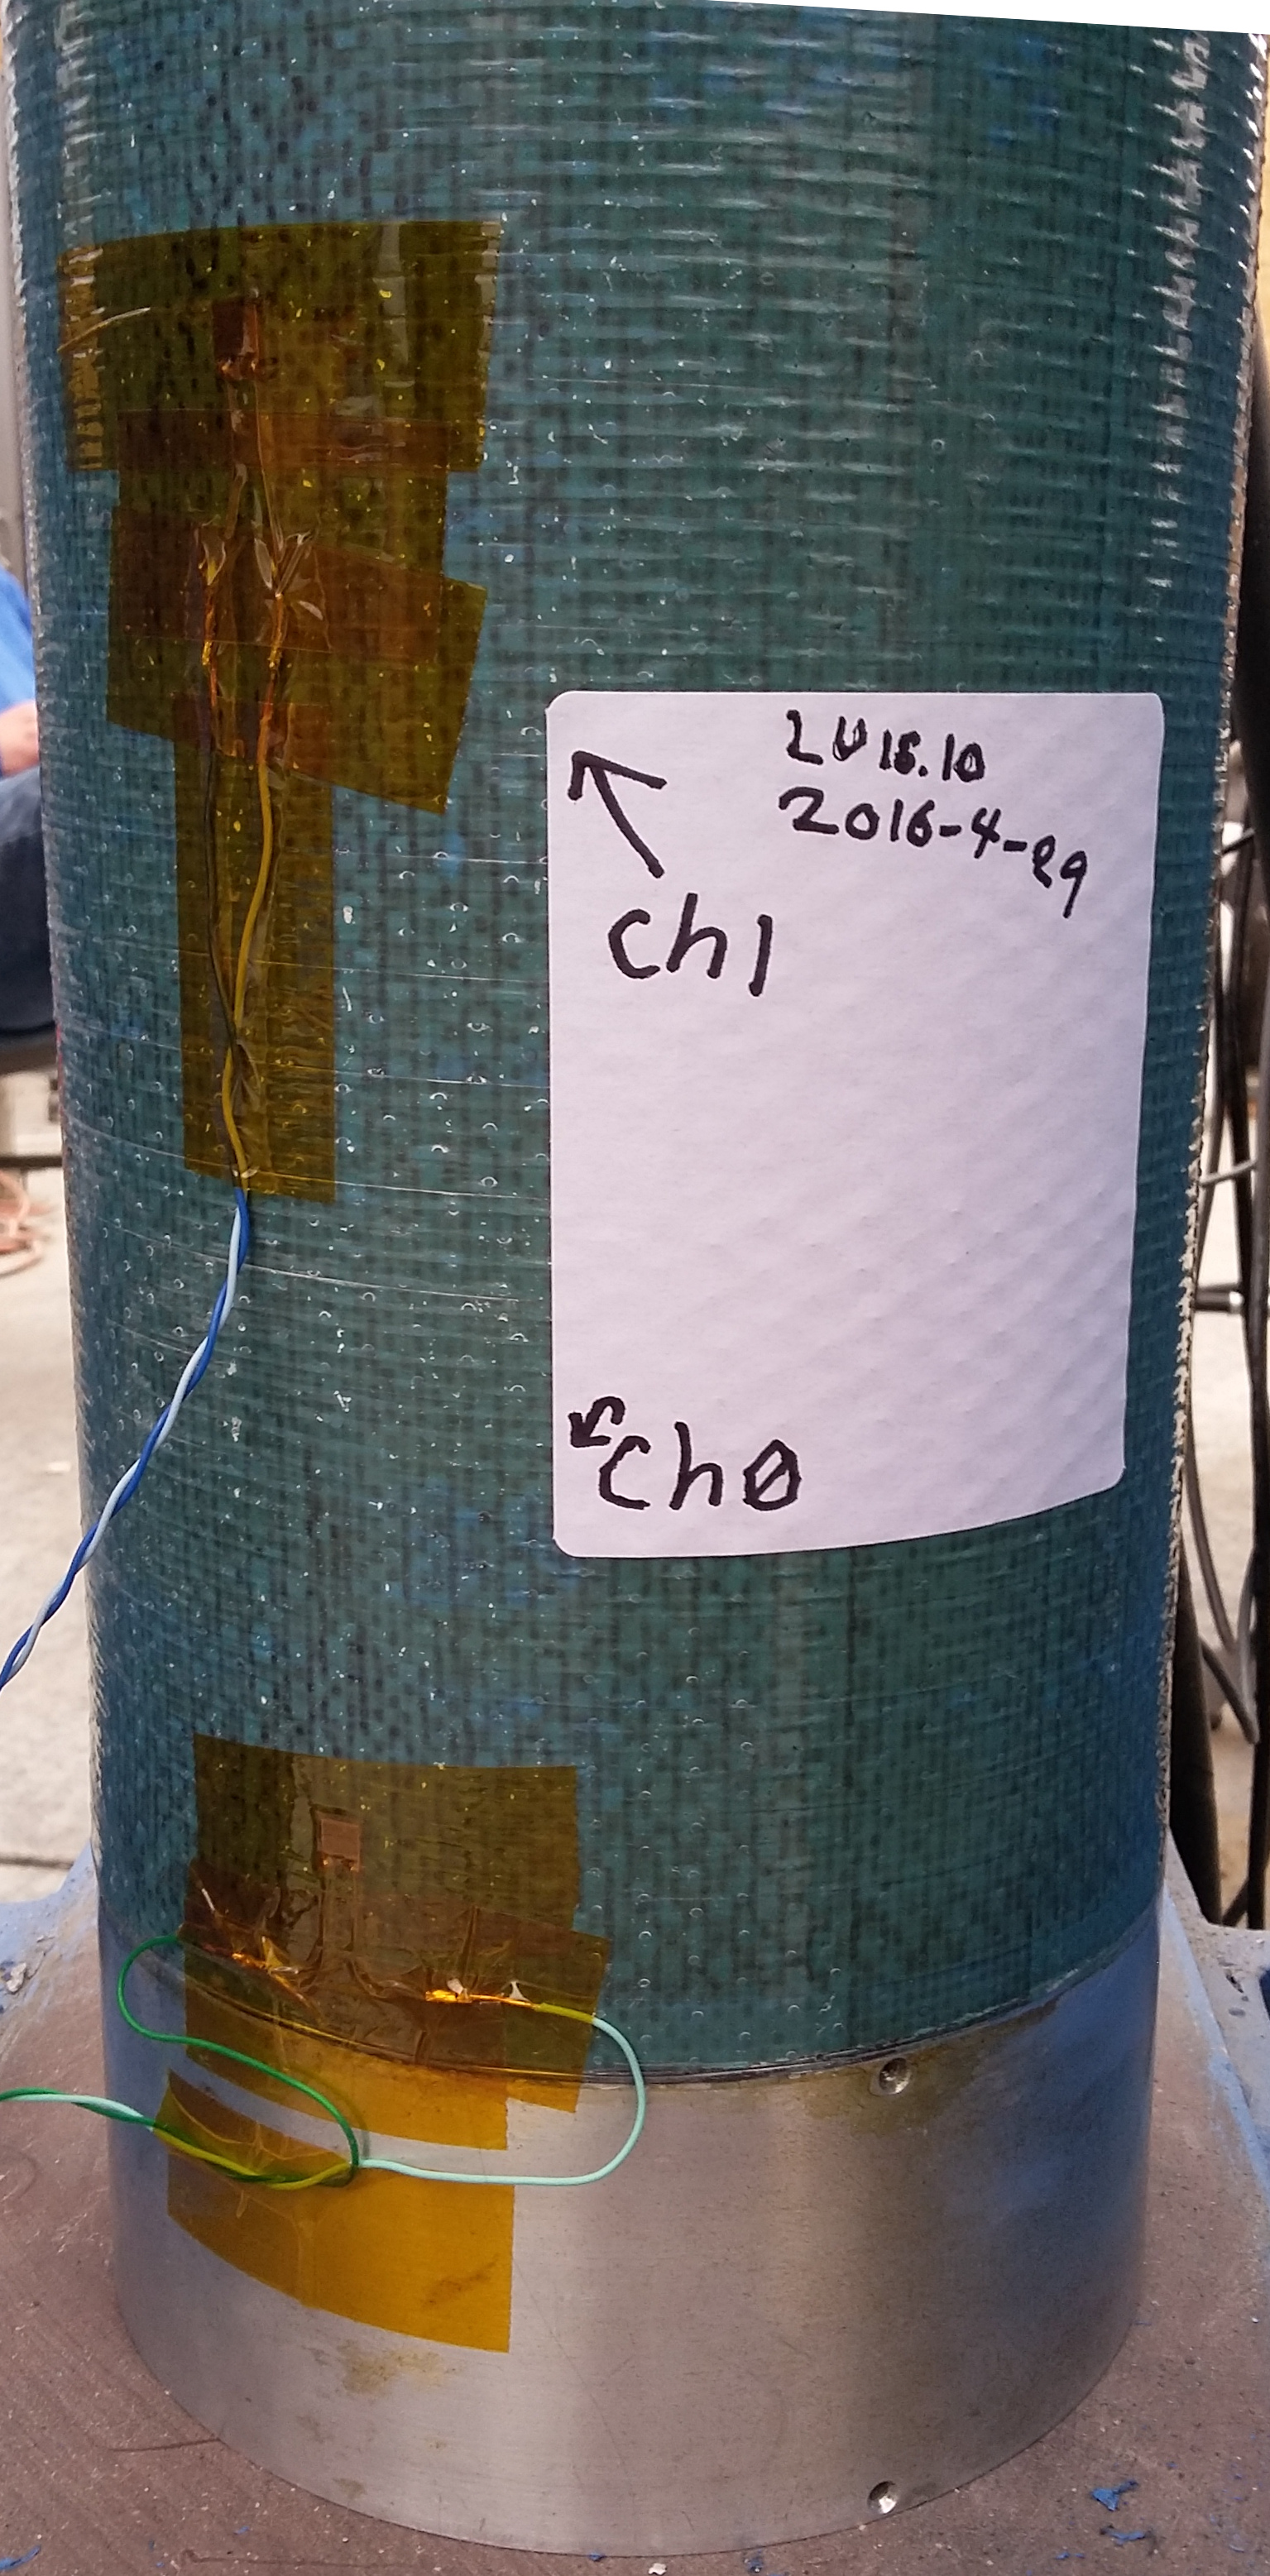
\includegraphics[width=\linewidth]{../img/LU16-10crush_close.jpg}
		\caption{
			Positioning of the strain gauges referred to in figure \ref{fig:strain}. 
			The gauges have been circled with colors corresponding to figure \ref{fig:strain}.
			Both are alligned with one of the pillars shown in figures \ref{fig:module} and \ref{fig:crush}.
			The bottom gauge is positioned directly above the point of failure.
			}
		\label{fig:gaugePosition}
	}
	\hfill
	\parbox{0.6\linewidth}
	{
		\centering
		% Created by tikzDevice version 0.10.1 on 2016-08-17 11:39:09.981
% !TEX encoding = UTF-8 Unicode
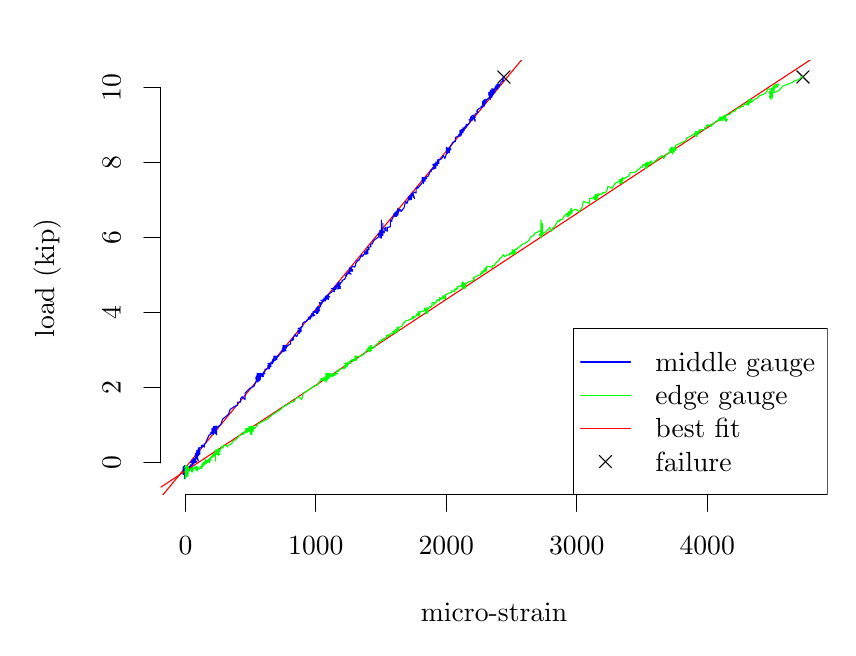
\begin{tikzpicture}[x=1pt,y=1pt]
\definecolor{fillColor}{RGB}{255,255,255}
\path[use as bounding box,fill=fillColor,fill opacity=0.00] (0,0) rectangle (289.08,216.81);
\begin{scope}
\path[clip] ( 48.00, 48.00) rectangle (289.08,204.81);

\path[] ( 57.28, 57.69) --
	( 56.74, 58.04) --
	( 56.74, 58.22) --
	( 56.74, 58.04) --
	( 56.19, 57.87) --
	( 56.74, 58.57) --
	( 56.19, 57.51) --
	( 56.74, 58.04) --
	( 56.74, 58.22) --
	( 56.74, 57.87) --
	( 56.74, 57.69) --
	( 56.74, 58.04) --
	( 57.28, 57.87) --
	( 56.74, 58.57) --
	( 56.74, 58.22) --
	( 56.74, 57.69) --
	( 57.28, 58.04) --
	( 56.19, 58.04) --
	( 56.74, 57.87) --
	( 57.28, 58.04) --
	( 56.19, 57.69) --
	( 57.28, 58.04) --
	( 56.74, 58.04) --
	( 56.74, 58.39) --
	( 57.28, 58.39) --
	( 56.74, 58.04) --
	( 56.19, 58.04) --
	( 56.74, 58.04) --
	( 57.28, 57.87) --
	( 56.74, 57.87) --
	( 57.28, 58.04) --
	( 57.28, 57.87) --
	( 56.74, 58.04) --
	( 57.28, 57.51) --
	( 57.28, 57.87) --
	( 56.74, 57.87) --
	( 57.28, 57.16) --
	( 56.74, 57.51) --
	( 56.74, 57.69) --
	( 57.28, 57.87) --
	( 56.74, 57.34) --
	( 56.74, 57.87) --
	( 56.74, 57.51) --
	( 56.74, 58.04) --
	( 56.74, 58.04) --
	( 56.74, 58.22) --
	( 56.74, 58.04) --
	( 56.74, 58.04) --
	( 56.19, 58.04) --
	( 56.74, 57.87) --
	( 56.74, 58.22) --
	( 56.74, 57.51) --
	( 56.74, 58.22) --
	( 56.74, 57.87) --
	( 56.74, 57.87) --
	( 56.74, 58.04) --
	( 56.19, 58.04) --
	( 56.74, 58.22) --
	( 56.74, 58.22) --
	( 56.19, 58.04) --
	( 56.74, 58.39) --
	( 56.74, 58.39) --
	( 56.74, 58.22) --
	( 56.74, 58.04) --
	( 56.74, 57.51) --
	( 56.74, 57.87) --
	( 56.74, 57.87) --
	( 56.74, 57.87) --
	( 57.28, 57.87) --
	( 57.28, 57.87) --
	( 56.74, 57.51) --
	( 56.74, 58.04) --
	( 56.19, 57.69) --
	( 56.74, 56.63) --
	( 56.74, 57.51) --
	( 56.74, 57.51) --
	( 56.74, 57.51) --
	( 56.74, 57.34) --
	( 56.74, 57.69) --
	( 57.28, 58.22) --
	( 57.28, 58.22) --
	( 56.74, 58.22) --
	( 56.74, 57.69) --
	( 56.74, 58.04) --
	( 56.74, 57.69) --
	( 56.74, 57.51) --
	( 57.28, 58.22) --
	( 56.19, 57.16) --
	( 56.74, 57.87) --
	( 56.74, 57.87) --
	( 56.74, 57.69) --
	( 56.74, 57.16) --
	( 56.19, 57.87) --
	( 56.74, 57.34) --
	( 57.28, 56.98) --
	( 57.28, 57.16) --
	( 56.74, 57.87) --
	( 57.28, 57.16) --
	( 56.19, 56.63) --
	( 56.74, 57.69) --
	( 57.28, 57.16) --
	( 56.19, 57.51) --
	( 56.74, 57.34) --
	( 56.74, 57.16) --
	( 56.74, 57.16) --
	( 56.74, 57.87) --
	( 56.74, 57.69) --
	( 57.28, 57.87) --
	( 56.74, 57.69) --
	( 56.74, 57.51) --
	( 56.19, 57.16) --
	( 56.74, 57.34) --
	( 56.74, 57.16) --
	( 57.28, 57.69) --
	( 56.74, 57.34) --
	( 56.74, 56.98) --
	( 56.74, 57.16) --
	( 56.74, 56.28) --
	( 56.74, 56.28) --
	( 56.74, 56.28) --
	( 56.74, 56.81) --
	( 56.19, 57.51) --
	( 56.74, 56.81) --
	( 56.74, 57.16) --
	( 56.74, 56.63) --
	( 57.28, 57.16) --
	( 56.74, 57.51) --
	( 56.74, 56.28) --
	( 56.19, 57.34) --
	( 56.74, 57.16) --
	( 56.74, 56.98) --
	( 56.74, 56.28) --
	( 56.74, 56.81) --
	( 56.74, 56.98) --
	( 56.74, 56.98) --
	( 56.74, 57.16) --
	( 57.28, 57.34) --
	( 57.28, 57.16) --
	( 56.74, 56.81) --
	( 56.19, 56.81) --
	( 56.74, 56.81) --
	( 57.28, 56.98) --
	( 56.74, 56.63) --
	( 57.28, 57.34) --
	( 56.74, 56.81) --
	( 56.74, 56.98) --
	( 57.28, 56.63) --
	( 56.74, 56.81) --
	( 56.74, 57.16) --
	( 57.28, 57.34) --
	( 56.74, 56.45) --
	( 56.74, 56.98) --
	( 56.74, 56.63) --
	( 57.28, 57.16) --
	( 56.74, 56.63) --
	( 56.74, 56.28) --
	( 56.19, 55.75) --
	( 57.28, 56.28) --
	( 56.74, 56.45) --
	( 56.19, 55.75) --
	( 57.28, 56.63) --
	( 56.74, 56.45) --
	( 57.28, 56.45) --
	( 56.74, 56.45) --
	( 56.74, 56.98) --
	( 56.74, 56.81) --
	( 56.74, 56.28) --
	( 56.74, 56.45) --
	( 56.74, 56.10) --
	( 56.74, 56.81) --
	( 56.74, 56.81) --
	( 56.74, 55.75) --
	( 57.28, 56.63) --
	( 57.28, 56.81) --
	( 56.19, 56.63) --
	( 56.74, 56.81) --
	( 56.74, 56.81) --
	( 57.28, 56.28) --
	( 57.28, 56.98) --
	( 56.74, 56.10) --
	( 56.19, 56.28) --
	( 56.74, 56.63) --
	( 56.74, 55.75) --
	( 56.74, 56.28) --
	( 56.74, 55.04) --
	( 57.28, 56.10) --
	( 56.74, 55.57) --
	( 56.74, 56.63) --
	( 56.19, 55.92) --
	( 57.28, 56.63) --
	( 56.74, 56.10) --
	( 56.74, 55.75) --
	( 56.74, 56.45) --
	( 57.28, 56.10) --
	( 56.74, 56.28) --
	( 56.74, 55.75) --
	( 56.19, 56.63) --
	( 57.28, 56.45) --
	( 56.74, 55.57) --
	( 56.74, 55.92) --
	( 57.28, 55.75) --
	( 56.74, 55.57) --
	( 56.74, 55.75) --
	( 56.74, 55.04) --
	( 57.28, 55.57) --
	( 56.74, 56.10) --
	( 56.74, 56.28) --
	( 56.74, 56.45) --
	( 57.28, 56.28) --
	( 56.74, 55.57) --
	( 56.19, 56.45) --
	( 57.28, 55.75) --
	( 57.28, 56.45) --
	( 57.28, 55.75) --
	( 56.19, 55.40) --
	( 56.74, 55.40) --
	( 57.28, 55.57) --
	( 57.28, 54.69) --
	( 56.74, 55.04) --
	( 56.74, 53.81) --
	( 56.74, 55.40) --
	( 56.74, 55.04) --
	( 56.74, 55.75) --
	( 56.74, 55.75) --
	( 56.74, 55.92) --
	( 56.74, 56.10) --
	( 57.28, 55.40) --
	( 56.74, 55.57) --
	( 57.28, 56.28) --
	( 56.19, 55.75) --
	( 56.74, 55.75) --
	( 56.74, 55.57) --
	( 56.74, 56.45) --
	( 56.74, 56.10) --
	( 57.28, 56.28) --
	( 56.74, 55.57) --
	( 57.28, 55.40) --
	( 57.28, 54.69) --
	( 56.74, 55.40) --
	( 57.28, 55.22) --
	( 57.28, 55.22) --
	( 56.74, 56.10) --
	( 57.28, 55.92) --
	( 57.28, 55.57) --
	( 56.74, 56.45) --
	( 57.28, 56.45) --
	( 57.28, 56.45) --
	( 56.74, 56.28) --
	( 56.19, 56.81) --
	( 56.74, 56.63) --
	( 56.74, 55.57) --
	( 56.74, 55.57) --
	( 56.74, 55.57) --
	( 56.74, 55.75) --
	( 56.74, 55.92) --
	( 56.74, 56.10) --
	( 56.74, 56.28) --
	( 57.28, 56.10) --
	( 57.28, 55.57) --
	( 56.74, 56.10) --
	( 56.74, 56.45) --
	( 56.74, 55.92) --
	( 56.74, 56.10) --
	( 56.74, 55.57) --
	( 56.74, 56.10) --
	( 56.74, 55.92) --
	( 56.74, 55.75) --
	( 57.28, 56.28) --
	( 56.74, 55.75) --
	( 57.28, 55.75) --
	( 56.74, 55.57) --
	( 56.74, 55.75) --
	( 56.19, 56.28) --
	( 57.28, 56.28) --
	( 56.74, 55.40) --
	( 57.28, 55.75) --
	( 57.28, 55.40) --
	( 57.28, 55.57) --
	( 56.74, 55.75) --
	( 56.74, 56.10) --
	( 56.74, 56.10) --
	( 56.74, 55.40) --
	( 56.74, 56.28) --
	( 56.74, 55.22) --
	( 56.74, 56.10) --
	( 56.74, 55.75) --
	( 56.74, 56.63) --
	( 57.28, 56.81) --
	( 56.19, 56.10) --
	( 56.19, 55.75) --
	( 56.74, 55.75) --
	( 57.28, 55.92) --
	( 56.74, 55.75) --
	( 57.28, 55.75) --
	( 56.74, 55.57) --
	( 56.74, 56.28) --
	( 56.74, 55.75) --
	( 57.28, 55.92) --
	( 56.19, 56.45) --
	( 56.74, 55.22) --
	( 57.28, 55.92) --
	( 56.74, 55.75) --
	( 57.28, 55.75) --
	( 56.74, 55.92) --
	( 56.74, 55.75) --
	( 56.74, 56.10) --
	( 56.74, 56.10) --
	( 56.74, 55.92) --
	( 56.74, 55.75) --
	( 57.28, 55.92) --
	( 57.28, 56.45) --
	( 56.74, 55.92) --
	( 56.74, 56.63) --
	( 56.19, 56.98) --
	( 56.74, 56.10) --
	( 56.74, 56.63) --
	( 57.28, 56.98) --
	( 57.28, 56.98) --
	( 57.28, 57.69) --
	( 57.28, 57.16) --
	( 57.28, 57.16) --
	( 57.83, 57.51) --
	( 57.28, 57.34) --
	( 57.28, 57.16) --
	( 57.83, 57.51) --
	( 57.83, 57.34) --
	( 57.83, 57.34) --
	( 57.28, 57.69) --
	( 57.83, 58.04) --
	( 57.83, 57.51) --
	( 57.83, 57.34) --
	( 57.83, 57.16) --
	( 57.83, 56.81) --
	( 57.83, 57.16) --
	( 57.83, 57.51) --
	( 57.83, 57.16) --
	( 57.83, 56.45) --
	( 57.83, 56.98) --
	( 57.28, 56.81) --
	( 57.28, 56.28) --
	( 57.28, 56.45) --
	( 57.28, 56.81) --
	( 57.83, 57.69) --
	( 57.28, 57.16) --
	( 57.83, 57.51) --
	( 57.28, 57.51) --
	( 57.83, 57.87) --
	( 57.28, 57.51) --
	( 57.28, 57.34) --
	( 57.83, 56.98) --
	( 57.28, 57.34) --
	( 57.28, 57.51) --
	( 57.28, 57.69) --
	( 57.28, 57.34) --
	( 57.83, 57.69) --
	( 57.83, 57.51) --
	( 57.83, 57.51) --
	( 57.83, 57.87) --
	( 58.38, 57.87) --
	( 57.28, 57.34) --
	( 57.83, 58.04) --
	( 57.28, 57.69) --
	( 57.28, 57.51) --
	( 57.28, 57.69) --
	( 57.83, 57.69) --
	( 57.28, 57.16) --
	( 57.83, 57.51) --
	( 58.38, 58.22) --
	( 57.83, 57.51) --
	( 58.38, 58.22) --
	( 58.38, 58.39) --
	( 58.92, 58.04) --
	( 58.92, 57.69) --
	( 58.38, 58.04) --
	( 58.38, 57.87) --
	( 58.38, 57.16) --
	( 58.38, 57.51) --
	( 58.38, 58.39) --
	( 58.38, 57.87) --
	( 57.83, 56.63) --
	( 57.83, 57.16) --
	( 58.38, 57.34) --
	( 58.38, 57.34) --
	( 58.38, 57.87) --
	( 57.83, 57.69) --
	( 58.38, 56.81) --
	( 58.38, 57.34) --
	( 57.83, 56.98) --
	( 58.38, 57.69) --
	( 58.38, 58.04) --
	( 58.38, 58.04) --
	( 58.38, 57.51) --
	( 58.38, 57.69) --
	( 58.38, 58.04) --
	( 58.38, 57.16) --
	( 58.38, 57.51) --
	( 58.38, 57.51) --
	( 58.38, 58.04) --
	( 58.38, 57.34) --
	( 58.38, 56.98) --
	( 58.38, 57.34) --
	( 57.83, 57.51) --
	( 58.38, 56.63) --
	( 57.83, 57.34) --
	( 58.38, 56.98) --
	( 58.38, 58.04) --
	( 58.92, 57.51) --
	( 58.38, 57.34) --
	( 58.38, 57.51) --
	( 58.92, 57.51) --
	( 58.92, 57.69) --
	( 59.47, 58.22) --
	( 58.92, 58.04) --
	( 59.47, 57.69) --
	( 58.92, 57.69) --
	( 58.92, 58.57) --
	( 59.47, 58.57) --
	( 59.47, 58.39) --
	( 59.47, 58.04) --
	( 59.47, 59.10) --
	( 59.47, 58.75) --
	( 58.92, 57.87) --
	( 58.92, 58.92) --
	( 58.92, 58.57) --
	( 59.47, 58.92) --
	( 59.47, 59.45) --
	( 59.47, 59.28) --
	( 59.47, 59.10) --
	( 59.47, 59.28) --
	( 59.47, 59.10) --
	( 59.47, 59.10) --
	( 59.47, 58.75) --
	( 59.47, 59.10) --
	( 59.47, 59.63) --
	( 60.02, 59.28) --
	( 60.02, 59.45) --
	( 60.02, 59.81) --
	( 59.47, 60.16) --
	( 59.47, 59.45) --
	( 60.02, 59.98) --
	( 60.02, 59.45) --
	( 59.47, 59.10) --
	( 59.47, 59.45) --
	( 59.47, 59.63) --
	( 60.02, 59.10) --
	( 59.47, 59.45) --
	( 58.92, 59.81) --
	( 59.47, 60.34) --
	( 59.47, 60.16) --
	( 59.47, 59.98) --
	( 59.47, 60.34) --
	( 60.02, 60.34) --
	( 59.47, 60.69) --
	( 60.02, 59.81) --
	( 60.56, 59.63) --
	( 60.02, 59.81) --
	( 60.02, 59.98) --
	( 60.02, 60.16) --
	( 60.02, 59.63) --
	( 60.02, 60.16) --
	( 60.56, 60.69) --
	( 59.47, 60.51) --
	( 60.02, 60.16) --
	( 60.02, 61.04) --
	( 60.02, 60.51) --
	( 60.56, 60.69) --
	( 60.02, 59.63) --
	( 60.02, 60.34) --
	( 61.11, 59.81) --
	( 60.02, 61.04) --
	( 61.11, 61.04) --
	( 61.11, 62.10) --
	( 60.56, 61.39) --
	( 61.11, 61.92) --
	( 60.56, 62.28) --
	( 61.66, 62.63) --
	( 61.11, 62.28) --
	( 61.11, 62.45) --
	( 61.11, 61.92) --
	( 61.11, 61.75) --
	( 60.56, 62.10) --
	( 60.56, 61.57) --
	( 61.11, 62.63) --
	( 60.56, 62.10) --
	( 61.66, 62.10) --
	( 61.11, 62.81) --
	( 60.56, 62.10) --
	( 61.66, 62.98) --
	( 61.11, 62.81) --
	( 61.11, 63.33) --
	( 61.11, 62.81) --
	( 60.56, 62.98) --
	( 61.66, 60.16) --
	( 61.11, 62.63) --
	( 61.66, 62.63) --
	( 61.11, 62.98) --
	( 61.66, 63.33) --
	( 61.11, 63.16) --
	( 61.11, 62.98) --
	( 61.66, 63.33) --
	( 61.66, 62.81) --
	( 61.66, 62.45) --
	( 61.11, 62.81) --
	( 61.66, 62.98) --
	( 61.11, 63.16) --
	( 61.66, 63.51) --
	( 61.66, 62.98) --
	( 61.11, 62.45) --
	( 61.11, 62.98) --
	( 61.11, 63.51) --
	( 61.66, 63.51) --
	( 61.66, 63.16) --
	( 61.11, 63.16) --
	( 61.66, 63.16) --
	( 61.66, 63.69) --
	( 61.11, 62.98) --
	( 61.66, 63.16) --
	( 61.11, 63.51) --
	( 61.11, 63.16) --
	( 61.66, 63.33) --
	( 61.66, 63.69) --
	( 61.11, 63.51) --
	( 61.11, 62.98) --
	( 61.11, 63.51) --
	( 61.11, 62.98) --
	( 61.66, 62.98) --
	( 61.66, 63.51) --
	( 61.66, 62.63) --
	( 61.11, 62.98) --
	( 61.66, 63.33) --
	( 61.66, 63.33) --
	( 61.66, 62.81) --
	( 61.66, 63.16) --
	( 61.11, 63.51) --
	( 61.66, 63.51) --
	( 61.11, 62.98) --
	( 61.11, 63.51) --
	( 61.66, 63.51) --
	( 61.66, 63.51) --
	( 61.11, 64.04) --
	( 61.66, 63.51) --
	( 61.66, 63.51) --
	( 61.11, 63.33) --
	( 61.66, 63.69) --
	( 61.66, 63.86) --
	( 61.66, 63.51) --
	( 61.66, 63.16) --
	( 61.66, 64.22) --
	( 61.66, 63.33) --
	( 61.66, 63.33) --
	( 61.66, 62.81) --
	( 61.66, 63.16) --
	( 61.66, 63.33) --
	( 61.66, 63.86) --
	( 61.11, 63.51) --
	( 61.66, 63.86) --
	( 61.11, 64.04) --
	( 61.66, 64.22) --
	( 61.66, 64.39) --
	( 61.66, 64.57) --
	( 61.66, 64.22) --
	( 61.66, 63.86) --
	( 61.66, 64.04) --
	( 61.66, 63.69) --
	( 61.66, 63.69) --
	( 61.66, 63.69) --
	( 61.11, 63.51) --
	( 62.20, 64.04) --
	( 61.66, 63.86) --
	( 61.66, 63.69) --
	( 61.66, 63.51) --
	( 62.20, 63.69) --
	( 61.66, 63.16) --
	( 61.11, 63.51) --
	( 62.20, 64.04) --
	( 61.66, 63.33) --
	( 61.11, 63.69) --
	( 61.66, 63.86) --
	( 61.66, 63.69) --
	( 61.66, 63.51) --
	( 61.66, 63.69) --
	( 61.66, 63.33) --
	( 61.66, 63.51) --
	( 61.66, 63.51) --
	( 61.66, 63.33) --
	( 61.66, 63.51) --
	( 62.20, 63.51) --
	( 62.20, 62.63) --
	( 61.11, 63.33) --
	( 61.66, 63.16) --
	( 61.11, 63.33) --
	( 61.11, 63.51) --
	( 61.66, 62.81) --
	( 61.66, 63.51) --
	( 61.66, 63.33) --
	( 61.66, 63.69) --
	( 61.11, 63.86) --
	( 61.66, 62.81) --
	( 61.66, 62.63) --
	( 61.66, 63.16) --
	( 61.66, 62.98) --
	( 61.66, 63.69) --
	( 61.66, 63.16) --
	( 61.66, 63.69) --
	( 61.66, 63.51) --
	( 61.66, 62.98) --
	( 61.66, 62.98) --
	( 61.66, 62.98) --
	( 61.66, 63.16) --
	( 61.66, 63.16) --
	( 61.66, 63.51) --
	( 61.66, 63.16) --
	( 62.20, 62.81) --
	( 61.11, 63.33) --
	( 61.66, 62.28) --
	( 61.66, 63.51) --
	( 61.66, 63.51) --
	( 61.66, 63.86) --
	( 61.66, 63.69) --
	( 61.66, 63.86) --
	( 61.66, 64.04) --
	( 61.66, 63.51) --
	( 62.20, 64.39) --
	( 61.66, 64.92) --
	( 62.75, 65.10) --
	( 62.75, 65.45) --
	( 62.75, 64.92) --
	( 63.30, 65.98) --
	( 62.75, 65.80) --
	( 63.84, 65.28) --
	( 63.84, 65.63) --
	( 63.84, 66.33) --
	( 64.39, 66.69) --
	( 64.39, 67.04) --
	( 64.94, 68.27) --
	( 65.48, 69.51) --
	( 66.03, 69.86) --
	( 66.58, 70.21) --
	( 66.03, 70.39) --
	( 66.58, 70.57) --
	( 66.58, 70.57) --
	( 67.12, 70.39) --
	( 66.58, 70.39) --
	( 66.58, 70.39) --
	( 66.58, 70.92) --
	( 67.12, 70.57) --
	( 67.12, 70.74) --
	( 66.58, 70.57) --
	( 66.58, 71.27) --
	( 67.12, 71.27) --
	( 66.58, 70.92) --
	( 67.12, 71.10) --
	( 67.12, 71.10) --
	( 66.58, 71.45) --
	( 66.58, 70.92) --
	( 67.12, 71.10) --
	( 67.12, 71.63) --
	( 67.12, 70.57) --
	( 67.12, 71.80) --
	( 67.12, 71.63) --
	( 67.12, 71.45) --
	( 67.12, 71.45) --
	( 67.12, 70.92) --
	( 67.12, 71.80) --
	( 67.12, 71.10) --
	( 67.12, 71.98) --
	( 67.12, 71.80) --
	( 67.12, 71.80) --
	( 67.12, 71.80) --
	( 67.12, 71.80) --
	( 67.12, 71.63) --
	( 67.12, 70.74) --
	( 67.12, 70.74) --
	( 67.12, 70.92) --
	( 67.67, 71.45) --
	( 66.58, 71.98) --
	( 67.12, 71.45) --
	( 67.12, 71.80) --
	( 67.12, 71.63) --
	( 66.58, 71.98) --
	( 67.12, 71.80) --
	( 67.12, 71.98) --
	( 67.12, 71.98) --
	( 67.12, 71.98) --
	( 67.12, 71.63) --
	( 67.12, 72.16) --
	( 67.67, 71.45) --
	( 67.12, 71.80) --
	( 67.67, 71.80) --
	( 67.67, 71.80) --
	( 67.12, 71.63) --
	( 67.12, 71.63) --
	( 67.67, 71.80) --
	( 67.67, 71.80) --
	( 67.12, 71.45) --
	( 66.58, 71.27) --
	( 67.67, 71.45) --
	( 67.12, 71.80) --
	( 67.12, 71.45) --
	( 67.12, 71.80) --
	( 67.12, 71.98) --
	( 67.12, 71.98) --
	( 67.12, 71.63) --
	( 67.12, 71.98) --
	( 67.12, 71.98) --
	( 67.12, 71.98) --
	( 67.12, 71.98) --
	( 67.67, 71.10) --
	( 67.67, 71.98) --
	( 67.12, 72.68) --
	( 67.12, 71.80) --
	( 67.12, 71.45) --
	( 67.12, 71.63) --
	( 67.12, 71.80) --
	( 67.67, 71.80) --
	( 67.12, 71.98) --
	( 67.12, 71.45) --
	( 67.12, 71.45) --
	( 67.12, 71.10) --
	( 67.12, 71.45) --
	( 67.67, 71.45) --
	( 67.67, 71.27) --
	( 67.12, 71.45) --
	( 67.67, 71.10) --
	( 67.67, 71.98) --
	( 67.12, 71.63) --
	( 67.67, 71.80) --
	( 67.12, 71.27) --
	( 67.67, 71.80) --
	( 67.12, 71.27) --
	( 67.12, 71.80) --
	( 67.67, 71.45) --
	( 67.12, 71.27) --
	( 67.67, 71.98) --
	( 67.67, 71.80) --
	( 67.12, 71.45) --
	( 67.12, 71.63) --
	( 67.12, 71.27) --
	( 67.67, 71.10) --
	( 67.12, 71.45) --
	( 67.12, 71.98) --
	( 67.67, 71.98) --
	( 67.12, 71.98) --
	( 68.22, 72.33) --
	( 67.12, 71.45) --
	( 68.22, 71.98) --
	( 67.67, 71.80) --
	( 67.67, 71.45) --
	( 67.12, 71.10) --
	( 67.12, 71.63) --
	( 67.12, 70.92) --
	( 67.67, 70.74) --
	( 67.67, 70.57) --
	( 67.12, 70.92) --
	( 66.58, 70.74) --
	( 67.12, 69.86) --
	( 67.67, 71.27) --
	( 67.67, 70.39) --
	( 67.67, 71.10) --
	( 67.12, 71.27) --
	( 67.67, 70.92) --
	( 67.12, 71.45) --
	( 67.12, 71.45) --
	( 66.58, 71.80) --
	( 67.67, 71.45) --
	( 67.67, 71.27) --
	( 67.67, 71.27) --
	( 67.12, 71.63) --
	( 67.67, 71.27) --
	( 67.12, 70.74) --
	( 67.67, 71.63) --
	( 67.67, 71.45) --
	( 67.12, 71.63) --
	( 67.67, 71.63) --
	( 67.67, 71.63) --
	( 67.12, 71.27) --
	( 67.12, 71.63) --
	( 67.67, 71.10) --
	( 67.12, 71.10) --
	( 67.67, 71.45) --
	( 67.12, 70.92) --
	( 67.12, 71.63) --
	( 67.67, 71.45) --
	( 68.22, 71.45) --
	( 67.67, 71.45) --
	( 67.12, 71.98) --
	( 67.12, 71.27) --
	( 67.67, 71.27) --
	( 67.67, 71.45) --
	( 67.67, 71.45) --
	( 67.67, 71.27) --
	( 67.67, 71.63) --
	( 67.67, 71.63) --
	( 67.67, 72.16) --
	( 67.67, 71.63) --
	( 67.67, 70.74) --
	( 67.12, 71.63) --
	( 67.67, 71.80) --
	( 67.67, 71.63) --
	( 67.12, 71.27) --
	( 67.12, 70.92) --
	( 68.22, 71.45) --
	( 67.12, 71.27) --
	( 67.12, 70.92) --
	( 67.12, 71.27) --
	( 67.67, 71.27) --
	( 67.12, 71.27) --
	( 67.67, 70.74) --
	( 67.67, 71.63) --
	( 67.67, 71.45) --
	( 67.67, 71.45) --
	( 67.67, 70.74) --
	( 67.12, 71.80) --
	( 67.12, 71.27) --
	( 67.12, 70.92) --
	( 67.67, 71.45) --
	( 67.12, 71.63) --
	( 67.67, 71.63) --
	( 67.12, 71.63) --
	( 67.12, 72.33) --
	( 67.67, 71.45) --
	( 67.12, 71.98) --
	( 67.12, 71.80) --
	( 67.12, 71.80) --
	( 67.12, 71.80) --
	( 67.12, 71.45) --
	( 67.67, 71.80) --
	( 68.22, 71.45) --
	( 67.12, 71.80) --
	( 67.67, 71.98) --
	( 67.67, 71.63) --
	( 67.12, 71.45) --
	( 67.67, 71.80) --
	( 67.67, 70.92) --
	( 67.12, 71.27) --
	( 67.12, 71.45) --
	( 67.12, 71.80) --
	( 67.12, 71.27) --
	( 67.12, 71.98) --
	( 67.12, 71.80) --
	( 67.67, 71.80) --
	( 67.12, 71.63) --
	( 67.12, 71.45) --
	( 67.12, 71.27) --
	( 67.67, 71.27) --
	( 67.67, 70.92) --
	( 67.67, 71.45) --
	( 67.67, 71.63) --
	( 67.67, 71.80) --
	( 68.22, 71.27) --
	( 67.67, 71.80) --
	( 67.12, 71.63) --
	( 67.67, 71.63) --
	( 67.67, 71.27) --
	( 67.12, 71.80) --
	( 67.67, 70.92) --
	( 67.67, 71.80) --
	( 67.12, 71.63) --
	( 67.67, 71.80) --
	( 67.67, 71.80) --
	( 67.12, 71.80) --
	( 67.12, 71.98) --
	( 67.12, 71.45) --
	( 67.12, 71.27) --
	( 67.12, 71.63) --
	( 67.67, 71.63) --
	( 67.67, 71.98) --
	( 67.12, 71.63) --
	( 67.67, 71.63) --
	( 67.12, 71.45) --
	( 67.12, 71.98) --
	( 67.12, 71.63) --
	( 67.12, 71.63) --
	( 67.67, 72.33) --
	( 67.12, 71.45) --
	( 67.67, 71.45) --
	( 67.12, 71.98) --
	( 67.67, 71.80) --
	( 67.67, 71.27) --
	( 67.12, 71.27) --
	( 67.12, 71.10) --
	( 67.12, 71.45) --
	( 67.67, 71.27) --
	( 67.67, 71.63) --
	( 67.12, 71.98) --
	( 67.12, 71.63) --
	( 67.67, 71.10) --
	( 67.67, 70.74) --
	( 67.12, 71.63) --
	( 68.22, 71.98) --
	( 67.12, 71.27) --
	( 67.12, 71.27) --
	( 67.12, 71.80) --
	( 67.12, 71.10) --
	( 67.12, 71.45) --
	( 67.67, 71.27) --
	( 67.67, 71.45) --
	( 67.67, 71.27) --
	( 67.67, 71.10) --
	( 67.67, 71.45) --
	( 67.12, 70.92) --
	( 67.67, 70.92) --
	( 67.67, 71.45) --
	( 67.67, 71.98) --
	( 67.67, 71.80) --
	( 67.67, 71.98) --
	( 67.67, 71.80) --
	( 67.67, 71.98) --
	( 67.12, 71.63) --
	( 67.67, 71.63) --
	( 67.67, 71.63) --
	( 67.12, 71.98) --
	( 67.12, 71.98) --
	( 67.67, 71.45) --
	( 67.12, 71.10) --
	( 67.12, 71.80) --
	( 67.12, 71.98) --
	( 67.67, 71.63) --
	( 67.67, 71.45) --
	( 67.67, 71.45) --
	( 67.67, 71.80) --
	( 67.67, 71.45) --
	( 67.12, 72.16) --
	( 68.22, 71.63) --
	( 68.22, 71.63) --
	( 67.12, 71.98) --
	( 67.12, 71.63) --
	( 67.67, 71.80) --
	( 67.67, 71.80) --
	( 67.12, 71.45) --
	( 67.12, 71.10) --
	( 67.12, 71.63) --
	( 67.67, 71.98) --
	( 67.12, 71.10) --
	( 67.67, 71.45) --
	( 67.67, 71.27) --
	( 67.67, 70.57) --
	( 67.12, 71.27) --
	( 67.67, 71.45) --
	( 67.67, 71.45) --
	( 67.67, 71.45) --
	( 67.67, 71.63) --
	( 67.12, 70.92) --
	( 67.12, 71.63) --
	( 67.67, 71.63) --
	( 67.67, 71.27) --
	( 67.12, 71.80) --
	( 67.12, 71.45) --
	( 67.12, 71.80) --
	( 67.67, 71.63) --
	( 67.12, 71.27) --
	( 67.67, 71.45) --
	( 67.67, 71.63) --
	( 67.67, 71.45) --
	( 67.67, 71.27) --
	( 67.67, 71.27) --
	( 67.67, 70.39) --
	( 67.67, 71.45) --
	( 67.67, 71.27) --
	( 67.67, 71.27) --
	( 67.12, 71.63) --
	( 67.12, 71.27) --
	( 67.12, 71.63) --
	( 68.22, 71.27) --
	( 67.67, 72.33) --
	( 67.12, 71.27) --
	( 67.12, 71.98) --
	( 67.67, 72.16) --
	( 67.67, 71.63) --
	( 68.22, 71.80) --
	( 67.67, 71.63) --
	( 67.12, 71.80) --
	( 67.12, 71.63) --
	( 68.22, 71.80) --
	( 67.67, 71.98) --
	( 67.67, 71.80) --
	( 67.67, 72.16) --
	( 67.12, 71.98) --
	( 67.67, 71.98) --
	( 67.67, 71.80) --
	( 67.67, 72.16) --
	( 67.12, 72.16) --
	( 67.12, 71.98) --
	( 67.67, 72.51) --
	( 67.67, 71.98) --
	( 67.12, 72.33) --
	( 67.67, 71.98) --
	( 67.67, 71.98) --
	( 67.67, 72.16) --
	( 67.67, 71.98) --
	( 67.67, 71.98) --
	( 67.67, 71.80) --
	( 67.67, 71.63) --
	( 67.67, 71.45) --
	( 67.67, 71.98) --
	( 67.12, 71.98) --
	( 68.22, 70.92) --
	( 67.67, 72.16) --
	( 67.12, 72.16) --
	( 67.67, 71.63) --
	( 67.67, 72.16) --
	( 67.12, 71.98) --
	( 67.67, 71.63) --
	( 67.12, 71.63) --
	( 67.67, 72.16) --
	( 67.12, 72.16) --
	( 67.67, 72.16) --
	( 67.67, 72.33) --
	( 67.12, 71.98) --
	( 67.12, 71.80) --
	( 67.67, 72.33) --
	( 67.67, 71.63) --
	( 67.67, 72.16) --
	( 67.12, 71.27) --
	( 67.12, 71.63) --
	( 67.12, 71.45) --
	( 68.22, 71.45) --
	( 67.67, 71.63) --
	( 67.67, 71.10) --
	( 67.12, 71.45) --
	( 67.12, 71.45) --
	( 67.67, 71.45) --
	( 67.67, 70.74) --
	( 68.22, 71.80) --
	( 67.12, 71.63) --
	( 67.12, 71.45) --
	( 67.67, 70.74) --
	( 67.67, 70.92) --
	( 68.22, 70.57) --
	( 68.22, 71.27) --
	( 67.12, 70.74) --
	( 67.67, 71.27) --
	( 68.22, 71.80) --
	( 67.12, 71.27) --
	( 67.67, 70.92) --
	( 68.22, 71.80) --
	( 67.12, 71.63) --
	( 67.67, 71.27) --
	( 67.12, 71.27) --
	( 67.67, 71.27) --
	( 68.22, 71.45) --
	( 67.67, 71.27) --
	( 67.67, 71.63) --
	( 67.12, 71.80) --
	( 67.12, 71.80) --
	( 67.12, 71.27) --
	( 68.22, 71.45) --
	( 68.22, 71.10) --
	( 68.22, 70.74) --
	( 67.67, 71.45) --
	( 67.12, 71.45) --
	( 68.22, 71.45) --
	( 67.67, 71.45) --
	( 67.12, 71.27) --
	( 67.67, 71.27) --
	( 67.67, 70.74) --
	( 67.67, 71.27) --
	( 67.12, 71.80) --
	( 67.67, 71.45) --
	( 67.12, 71.80) --
	( 67.67, 71.80) --
	( 67.12, 71.45) --
	( 67.67, 71.98) --
	( 67.12, 71.98) --
	( 67.67, 71.45) --
	( 67.67, 71.98) --
	( 68.22, 71.63) --
	( 67.67, 71.98) --
	( 67.67, 71.98) --
	( 67.12, 71.63) --
	( 68.22, 71.98) --
	( 67.67, 70.57) --
	( 67.67, 71.63) --
	( 67.12, 71.98) --
	( 67.67, 72.16) --
	( 67.12, 72.51) --
	( 67.12, 72.16) --
	( 67.67, 72.68) --
	( 67.12, 72.33) --
	( 67.67, 72.16) --
	( 67.12, 72.16) --
	( 67.67, 72.51) --
	( 67.67, 72.33) --
	( 67.12, 72.16) --
	( 67.67, 71.98) --
	( 67.12, 72.16) --
	( 67.12, 72.33) --
	( 67.67, 72.16) --
	( 68.22, 71.98) --
	( 67.67, 71.98) --
	( 68.22, 71.80) --
	( 67.12, 71.98) --
	( 67.67, 71.27) --
	( 67.67, 71.45) --
	( 67.12, 71.63) --
	( 67.67, 71.63) --
	( 67.12, 71.80) --
	( 68.22, 71.63) --
	( 67.67, 72.16) --
	( 67.12, 71.98) --
	( 67.67, 71.80) --
	( 67.67, 71.98) --
	( 68.22, 71.27) --
	( 67.67, 71.63) --
	( 67.67, 70.92) --
	( 67.67, 71.45) --
	( 68.22, 71.10) --
	( 67.67, 70.74) --
	( 67.67, 71.27) --
	( 67.67, 71.45) --
	( 67.67, 71.45) --
	( 67.12, 71.45) --
	( 67.67, 71.45) --
	( 67.67, 70.92) --
	( 68.22, 71.63) --
	( 68.22, 71.63) --
	( 67.12, 71.10) --
	( 67.12, 71.63) --
	( 67.12, 70.92) --
	( 67.67, 71.63) --
	( 67.67, 71.45) --
	( 67.67, 71.80) --
	( 67.67, 70.74) --
	( 67.67, 70.57) --
	( 67.12, 71.10) --
	( 67.12, 71.10) --
	( 68.22, 71.45) --
	( 67.67, 71.27) --
	( 67.67, 71.10) --
	( 67.12, 71.63) --
	( 67.67, 71.45) --
	( 67.67, 71.45) --
	( 67.67, 71.27) --
	( 67.12, 71.45) --
	( 67.67, 71.45) --
	( 67.67, 71.98) --
	( 67.67, 71.45) --
	( 67.67, 70.92) --
	( 67.67, 71.27) --
	( 67.67, 71.27) --
	( 67.12, 71.80) --
	( 67.67, 71.80) --
	( 67.67, 71.63) --
	( 67.67, 72.33) --
	( 67.67, 72.51) --
	( 67.67, 72.33) --
	( 68.22, 72.68) --
	( 67.67, 72.33) --
	( 67.67, 71.63) --
	( 67.67, 72.16) --
	( 67.67, 71.98) --
	( 67.67, 71.98) --
	( 67.67, 71.63) --
	( 68.22, 72.51) --
	( 67.67, 71.98) --
	( 67.67, 72.33) --
	( 67.67, 71.27) --
	( 68.22, 71.80) --
	( 67.67, 71.98) --
	( 67.67, 71.98) --
	( 68.22, 72.33) --
	( 67.67, 71.45) --
	( 67.67, 71.98) --
	( 68.22, 72.16) --
	( 67.67, 72.33) --
	( 67.67, 72.16) --
	( 67.12, 72.51) --
	( 67.67, 71.98) --
	( 67.67, 72.33) --
	( 67.67, 71.63) --
	( 68.22, 72.16) --
	( 67.67, 72.16) --
	( 68.22, 71.98) --
	( 68.22, 71.63) --
	( 67.67, 71.45) --
	( 67.67, 71.80) --
	( 67.67, 72.16) --
	( 68.22, 71.63) --
	( 67.67, 71.45) --
	( 67.67, 71.98) --
	( 67.67, 71.98) --
	( 67.67, 71.80) --
	( 67.12, 71.45) --
	( 67.12, 71.27) --
	( 68.22, 71.98) --
	( 67.12, 71.63) --
	( 67.67, 71.80) --
	( 67.67, 71.98) --
	( 67.67, 71.45) --
	( 68.22, 71.98) --
	( 67.67, 71.63) --
	( 67.67, 71.98) --
	( 68.22, 71.80) --
	( 67.67, 71.80) --
	( 67.67, 70.92) --
	( 67.12, 71.45) --
	( 67.67, 70.74) --
	( 67.67, 71.45) --
	( 68.22, 71.45) --
	( 67.12, 71.80) --
	( 67.67, 71.63) --
	( 67.67, 72.16) --
	( 67.67, 71.98) --
	( 67.67, 71.98) --
	( 67.67, 71.98) --
	( 67.67, 71.80) --
	( 67.67, 71.98) --
	( 67.12, 71.98) --
	( 67.67, 72.51) --
	( 67.67, 72.68) --
	( 68.22, 71.80) --
	( 67.67, 72.33) --
	( 67.67, 72.51) --
	( 68.22, 71.98) --
	( 67.12, 71.98) --
	( 67.67, 71.98) --
	( 67.12, 71.63) --
	( 67.12, 71.45) --
	( 68.22, 72.16) --
	( 67.67, 72.16) --
	( 67.12, 71.80) --
	( 68.22, 70.92) --
	( 67.67, 71.10) --
	( 67.67, 71.10) --
	( 67.67, 71.27) --
	( 68.22, 70.92) --
	( 67.12, 71.10) --
	( 68.22, 71.80) --
	( 67.12, 72.33) --
	( 68.22, 71.98) --
	( 67.67, 72.16) --
	( 67.12, 71.63) --
	( 67.67, 72.33) --
	( 67.67, 71.45) --
	( 67.67, 71.80) --
	( 67.67, 71.63) --
	( 67.12, 71.27) --
	( 68.22, 71.45) --
	( 67.67, 71.45) --
	( 67.67, 70.74) --
	( 67.67, 71.27) --
	( 67.67, 71.63) --
	( 67.12, 72.16) --
	( 67.67, 71.80) --
	( 67.12, 71.98) --
	( 67.67, 71.80) --
	( 67.12, 71.98) --
	( 67.67, 72.33) --
	( 67.12, 72.33) --
	( 67.12, 72.33) --
	( 67.67, 71.63) --
	( 68.22, 71.80) --
	( 67.67, 71.98) --
	( 67.67, 71.63) --
	( 67.12, 71.63) --
	( 68.22, 71.63) --
	( 67.67, 71.98) --
	( 68.22, 72.33) --
	( 67.67, 71.98) --
	( 67.12, 71.63) --
	( 68.22, 71.80) --
	( 68.22, 71.63) --
	( 67.12, 72.16) --
	( 67.67, 72.16) --
	( 67.67, 72.16) --
	( 67.12, 72.16) --
	( 67.12, 72.16) --
	( 67.12, 72.68) --
	( 67.67, 72.51) --
	( 67.67, 71.98) --
	( 67.67, 72.51) --
	( 67.67, 71.80) --
	( 67.12, 72.33) --
	( 68.22, 71.63) --
	( 67.12, 72.33) --
	( 67.67, 72.16) --
	( 67.67, 72.33) --
	( 67.12, 71.80) --
	( 67.12, 71.98) --
	( 67.12, 71.80) --
	( 67.67, 71.80) --
	( 67.12, 71.98) --
	( 67.12, 72.16) --
	( 67.67, 71.98) --
	( 67.67, 71.98) --
	( 67.67, 72.51) --
	( 68.22, 71.98) --
	( 67.67, 72.16) --
	( 67.12, 71.45) --
	( 67.67, 71.45) --
	( 68.22, 71.98) --
	( 67.67, 71.98) --
	( 68.22, 71.98) --
	( 67.12, 71.63) --
	( 68.22, 71.45) --
	( 67.67, 71.63) --
	( 67.12, 72.33) --
	( 67.67, 71.80) --
	( 67.12, 71.98) --
	( 67.67, 72.16) --
	( 67.67, 71.80) --
	( 67.67, 72.16) --
	( 67.12, 71.63) --
	( 67.67, 71.98) --
	( 67.67, 72.68) --
	( 67.67, 71.80) --
	( 67.67, 72.16) --
	( 67.67, 71.63) --
	( 67.12, 71.63) --
	( 67.67, 72.68) --
	( 68.22, 72.16) --
	( 68.22, 71.98) --
	( 67.67, 72.33) --
	( 67.67, 72.16) --
	( 67.67, 72.33) --
	( 68.22, 71.80) --
	( 68.22, 71.80) --
	( 67.67, 71.80) --
	( 67.67, 72.16) --
	( 68.22, 72.33) --
	( 67.67, 72.51) --
	( 67.67, 72.33) --
	( 67.67, 72.51) --
	( 67.67, 72.68) --
	( 67.67, 72.68) --
	( 67.67, 72.33) --
	( 68.22, 72.33) --
	( 67.12, 72.68) --
	( 67.67, 72.51) --
	( 67.67, 72.16) --
	( 67.67, 72.16) --
	( 67.12, 72.51) --
	( 68.22, 72.33) --
	( 67.67, 72.51) --
	( 67.67, 72.33) --
	( 68.22, 71.98) --
	( 68.22, 71.98) --
	( 67.67, 71.98) --
	( 67.67, 72.51) --
	( 67.67, 72.16) --
	( 68.22, 72.86) --
	( 68.22, 72.68) --
	( 67.67, 72.16) --
	( 67.67, 72.33) --
	( 67.12, 72.68) --
	( 67.67, 72.68) --
	( 67.67, 72.68) --
	( 68.22, 72.86) --
	( 68.22, 72.51) --
	( 67.67, 72.33) --
	( 68.22, 72.16) --
	( 68.22, 72.33) --
	( 67.67, 71.98) --
	( 67.67, 71.98) --
	( 68.22, 72.33) --
	( 67.67, 72.51) --
	( 67.12, 72.68) --
	( 67.67, 72.33) --
	( 68.22, 72.68) --
	( 67.12, 72.68) --
	( 67.67, 72.16) --
	( 68.22, 72.68) --
	( 68.22, 72.33) --
	( 67.12, 72.68) --
	( 67.67, 72.51) --
	( 67.67, 72.33) --
	( 67.67, 72.16) --
	( 67.67, 71.98) --
	( 67.67, 72.51) --
	( 67.67, 72.16) --
	( 68.22, 72.16) --
	( 67.67, 71.63) --
	( 68.22, 72.16) --
	( 67.67, 72.51) --
	( 68.22, 72.16) --
	( 67.12, 72.33) --
	( 67.67, 72.16) --
	( 67.67, 71.63) --
	( 67.12, 71.98) --
	( 67.67, 71.45) --
	( 67.67, 71.80) --
	( 67.67, 71.27) --
	( 67.67, 71.45) --
	( 67.12, 71.63) --
	( 68.22, 69.69) --
	( 68.22, 71.27) --
	( 67.12, 71.80) --
	( 67.67, 71.27) --
	( 68.22, 70.92) --
	( 67.67, 72.16) --
	( 67.67, 71.45) --
	( 67.12, 71.63) --
	( 67.67, 71.80) --
	( 68.22, 71.45) --
	( 67.12, 71.63) --
	( 67.12, 71.80) --
	( 68.22, 71.45) --
	( 67.67, 71.98) --
	( 67.67, 71.10) --
	( 68.22, 71.80) --
	( 67.12, 71.98) --
	( 67.67, 71.80) --
	( 68.22, 71.45) --
	( 68.22, 71.63) --
	( 67.67, 72.33) --
	( 68.22, 71.80) --
	( 68.22, 71.98) --
	( 69.86, 73.57) --
	( 70.40, 75.33) --
	( 72.59, 77.10) --
	( 73.14, 78.86) --
	( 74.78, 79.92) --
	( 75.87, 80.45) --
	( 75.87, 81.51) --
	( 76.96, 81.51) --
	( 76.96, 81.86) --
	( 76.96, 82.74) --
	( 77.51, 83.45) --
	( 78.60, 82.39) --
	( 78.60, 84.86) --
	( 79.15, 85.39) --
	( 80.24, 86.45) --
	( 81.88, 87.33) --
	( 81.88, 87.50) --
	( 82.97, 89.97) --
	( 82.43, 89.80) --
	( 82.97, 89.80) --
	( 82.43, 90.15) --
	( 82.97, 89.97) --
	( 82.97, 90.15) --
	( 82.97, 89.80) --
	( 82.97, 89.97) --
	( 82.97, 89.44) --
	( 82.97, 89.44) --
	( 82.97, 89.62) --
	( 82.97, 89.62) --
	( 82.97, 89.27) --
	( 82.97, 89.62) --
	( 82.97, 89.62) --
	( 82.97, 89.80) --
	( 83.52, 89.44) --
	( 83.52, 90.33) --
	( 82.97, 89.62) --
	( 83.52, 90.15) --
	( 84.07, 89.80) --
	( 83.52, 89.09) --
	( 82.43, 90.15) --
	( 83.52, 89.97) --
	( 82.97, 89.97) --
	( 83.52, 90.33) --
	( 82.97, 89.27) --
	( 83.52, 90.15) --
	( 82.97, 90.33) --
	( 83.52, 90.33) --
	( 83.52, 89.97) --
	( 83.52, 90.33) --
	( 83.52, 89.97) --
	( 82.97, 90.33) --
	( 83.52, 90.15) --
	( 83.52, 90.50) --
	( 83.52, 90.33) --
	( 82.97, 88.74) --
	( 83.52, 89.62) --
	( 83.52, 90.50) --
	( 83.52, 90.33) --
	( 83.52, 90.50) --
	( 82.97, 91.03) --
	( 83.52, 90.68) --
	( 82.97, 90.86) --
	( 83.52, 90.33) --
	( 82.97, 91.21) --
	( 82.43, 90.33) --
	( 82.97, 90.50) --
	( 82.97, 90.68) --
	( 83.52, 90.33) --
	( 83.52, 91.03) --
	( 82.97, 90.68) --
	( 82.97, 90.15) --
	( 83.52, 90.33) --
	( 82.97, 90.68) --
	( 83.52, 89.62) --
	( 84.07, 90.50) --
	( 83.52, 89.62) --
	( 83.52, 89.62) --
	( 83.52, 90.15) --
	( 83.52, 90.15) --
	( 83.52, 89.97) --
	( 83.52, 89.80) --
	( 83.52, 90.33) --
	( 83.52, 90.68) --
	( 83.52, 90.50) --
	( 83.52, 91.03) --
	( 83.52, 90.50) --
	( 83.52, 90.68) --
	( 83.52, 90.50) --
	( 84.07, 91.39) --
	( 83.52, 91.03) --
	( 82.97, 90.68) --
	( 83.52, 90.68) --
	( 82.97, 91.03) --
	( 83.52, 90.68) --
	( 83.52, 90.86) --
	( 83.52, 91.21) --
	( 83.52, 91.03) --
	( 83.52, 90.86) --
	( 83.52, 90.68) --
	( 83.52, 91.03) --
	( 82.97, 91.03) --
	( 82.97, 90.15) --
	( 83.52, 91.03) --
	( 83.52, 91.21) --
	( 84.07, 91.91) --
	( 82.97, 91.91) --
	( 82.97, 91.21) --
	( 83.52, 91.56) --
	( 83.52, 91.91) --
	( 83.52, 91.56) --
	( 83.52, 91.03) --
	( 82.97, 91.03) --
	( 83.52, 91.21) --
	( 83.52, 91.21) --
	( 82.97, 90.50) --
	( 83.52, 90.68) --
	( 83.52, 90.15) --
	( 83.52, 90.50) --
	( 83.52, 90.15) --
	( 83.52, 89.62) --
	( 83.52, 90.33) --
	( 83.52, 90.15) --
	( 84.07, 90.33) --
	( 83.52, 90.33) --
	( 83.52, 90.33) --
	( 83.52, 90.15) --
	( 83.52, 90.15) --
	( 82.97, 90.33) --
	( 84.07, 90.50) --
	( 83.52, 90.33) --
	( 84.07, 90.15) --
	( 82.97, 90.86) --
	( 83.52, 89.97) --
	( 83.52, 90.15) --
	( 84.07, 90.33) --
	( 83.52, 90.68) --
	( 83.52, 90.15) --
	( 83.52, 90.86) --
	( 82.97, 90.50) --
	( 83.52, 90.68) --
	( 82.97, 90.68) --
	( 83.52, 90.68) --
	( 82.97, 90.68) --
	( 83.52, 90.50) --
	( 83.52, 90.86) --
	( 82.97, 90.68) --
	( 84.07, 90.86) --
	( 83.52, 90.68) --
	( 84.07, 90.68) --
	( 83.52, 90.86) --
	( 83.52, 90.86) --
	( 83.52, 90.50) --
	( 83.52, 90.33) --
	( 83.52, 90.50) --
	( 84.07, 90.68) --
	( 84.07, 91.03) --
	( 83.52, 90.68) --
	( 83.52, 90.50) --
	( 83.52, 90.50) --
	( 84.07, 90.68) --
	( 83.52, 90.50) --
	( 83.52, 90.50) --
	( 83.52, 90.33) --
	( 83.52, 90.33) --
	( 83.52, 90.68) --
	( 83.52, 90.33) --
	( 84.07, 90.15) --
	( 84.07, 90.50) --
	( 82.97, 90.68) --
	( 84.07, 90.86) --
	( 84.07, 90.86) --
	( 83.52, 91.21) --
	( 84.07, 91.03) --
	( 83.52, 91.56) --
	( 83.52, 91.03) --
	( 83.52, 90.86) --
	( 83.52, 91.39) --
	( 83.52, 90.68) --
	( 84.07, 91.03) --
	( 83.52, 91.03) --
	( 83.52, 91.03) --
	( 83.52, 90.68) --
	( 83.52, 90.68) --
	( 84.07, 90.33) --
	( 83.52, 90.68) --
	( 83.52, 90.86) --
	( 83.52, 90.68) --
	( 84.07, 90.68) --
	( 83.52, 90.33) --
	( 84.07, 91.03) --
	( 84.07, 91.21) --
	( 83.52, 91.21) --
	( 83.52, 90.86) --
	( 84.07, 90.50) --
	( 83.52, 90.68) --
	( 83.52, 90.68) --
	( 84.07, 91.03) --
	( 83.52, 91.03) --
	( 83.52, 90.50) --
	( 84.07, 90.86) --
	( 84.07, 91.21) --
	( 84.07, 90.86) --
	( 84.07, 90.68) --
	( 84.07, 90.86) --
	( 84.07, 90.68) --
	( 82.97, 91.03) --
	( 83.52, 91.21) --
	( 83.52, 90.86) --
	( 83.52, 90.33) --
	( 84.07, 90.50) --
	( 83.52, 91.03) --
	( 83.52, 91.03) --
	( 83.52, 91.03) --
	( 84.07, 90.68) --
	( 83.52, 91.03) --
	( 83.52, 90.50) --
	( 83.52, 90.86) --
	( 83.52, 90.68) --
	( 83.52, 90.86) --
	( 83.52, 91.74) --
	( 83.52, 91.21) --
	( 83.52, 91.03) --
	( 83.52, 91.91) --
	( 82.97, 90.68) --
	( 84.07, 91.03) --
	( 84.07, 91.21) --
	( 83.52, 91.21) --
	( 84.07, 91.03) --
	( 83.52, 91.03) --
	( 83.52, 90.86) --
	( 84.07, 91.21) --
	( 84.07, 91.21) --
	( 83.52, 91.39) --
	( 83.52, 90.68) --
	( 83.52, 91.39) --
	( 84.07, 90.86) --
	( 83.52, 91.03) --
	( 83.52, 91.39) --
	( 83.52, 90.68) --
	( 83.52, 91.03) --
	( 83.52, 91.03) --
	( 84.07, 90.33) --
	( 83.52, 91.03) --
	( 84.07, 90.50) --
	( 83.52, 91.21) --
	( 83.52, 90.33) --
	( 83.52, 91.56) --
	( 84.07, 90.33) --
	( 83.52, 90.86) --
	( 83.52, 91.03) --
	( 83.52, 91.39) --
	( 83.52, 91.03) --
	( 82.97, 91.03) --
	( 84.07, 90.68) --
	( 84.07, 91.03) --
	( 84.07, 90.68) --
	( 84.07, 91.56) --
	( 83.52, 91.21) --
	( 83.52, 91.39) --
	( 84.07, 91.39) --
	( 83.52, 90.86) --
	( 84.07, 91.39) --
	( 83.52, 89.97) --
	( 84.07, 90.50) --
	( 83.52, 90.50) --
	( 84.07, 90.50) --
	( 83.52, 90.86) --
	( 83.52, 90.68) --
	( 84.07, 90.86) --
	( 83.52, 91.03) --
	( 84.07, 91.03) --
	( 83.52, 91.21) --
	( 83.52, 90.33) --
	( 83.52, 91.03) --
	( 83.52, 90.68) --
	( 83.52, 90.50) --
	( 84.07, 90.68) --
	( 84.07, 90.68) --
	( 84.07, 91.21) --
	( 84.07, 91.21) --
	( 84.07, 91.21) --
	( 84.07, 91.39) --
	( 84.07, 91.39) --
	( 83.52, 91.03) --
	( 84.07, 91.39) --
	( 84.07, 91.74) --
	( 84.07, 91.56) --
	( 83.52, 91.39) --
	( 84.07, 91.91) --
	( 84.07, 91.21) --
	( 84.61, 91.03) --
	( 84.07, 91.56) --
	( 84.07, 91.74) --
	( 84.07, 91.56) --
	( 84.61, 91.39) --
	( 84.61, 91.74) --
	( 84.07, 91.39) --
	( 84.61, 91.74) --
	( 84.07, 91.74) --
	( 84.61, 91.56) --
	( 84.61, 91.56) --
	( 84.61, 91.21) --
	( 84.61, 91.74) --
	( 84.07, 90.86) --
	( 84.61, 91.21) --
	( 85.16, 90.68) --
	( 84.61, 90.86) --
	( 84.61, 91.56) --
	( 84.61, 91.74) --
	( 84.61, 91.39) --
	( 84.61, 91.39) --
	( 84.61, 91.21) --
	( 85.16, 91.21) --
	( 84.61, 91.74) --
	( 84.61, 91.39) --
	( 84.61, 91.74) --
	( 85.71, 91.74) --
	( 85.16, 91.74) --
	( 85.71, 91.91) --
	( 85.16, 91.91) --
	( 85.71, 91.91) --
	( 85.16, 91.74) --
	( 85.16, 92.27) --
	( 85.16, 92.09) --
	( 85.71, 92.80) --
	( 85.71, 92.62) --
	( 85.71, 93.33) --
	( 86.25, 93.50) --
	( 86.25, 93.50) --
	( 86.25, 93.50) --
	( 87.35, 93.50) --
	( 87.35, 93.86) --
	( 87.35, 94.91) --
	( 86.80, 93.86) --
	( 86.80, 94.74) --
	( 87.89, 94.38) --
	( 87.35, 94.56) --
	( 87.35, 94.56) --
	( 87.35, 94.74) --
	( 87.35, 94.03) --
	( 87.89, 94.56) --
	( 87.35, 94.38) --
	( 87.35, 94.38) --
	( 87.89, 94.91) --
	( 87.89, 94.38) --
	( 87.35, 94.56) --
	( 87.35, 94.91) --
	( 87.35, 94.21) --
	( 87.89, 95.27) --
	( 87.35, 94.74) --
	( 87.89, 95.27) --
	( 87.89, 95.09) --
	( 87.89, 95.44) --
	( 87.89, 95.44) --
	( 86.80, 95.44) --
	( 87.89, 94.74) --
	( 87.89, 94.91) --
	( 87.89, 95.09) --
	( 87.89, 95.44) --
	( 87.89, 94.74) --
	( 87.35, 95.09) --
	( 87.35, 95.09) --
	( 87.35, 94.91) --
	( 87.35, 95.09) --
	( 87.89, 94.91) --
	( 87.89, 95.09) --
	( 87.35, 94.74) --
	( 87.35, 94.91) --
	( 87.89, 95.80) --
	( 87.89, 95.80) --
	( 87.89, 95.09) --
	( 87.89, 95.80) --
	( 88.44, 96.15) --
	( 88.44, 95.44) --
	( 88.99, 96.50) --
	( 88.99, 96.50) --
	( 88.44, 96.68) --
	( 88.99, 96.33) --
	( 88.44, 96.50) --
	( 88.44, 96.68) --
	( 88.44, 96.50) --
	( 88.99, 96.85) --
	( 88.99, 96.85) --
	( 88.44, 96.68) --
	( 88.99, 97.38) --
	( 88.99, 97.38) --
	( 90.08, 98.09) --
	( 89.53, 97.56) --
	( 88.99, 97.74) --
	( 88.99, 98.09) --
	( 88.99, 97.56) --
	( 89.53, 97.56) --
	( 90.08, 98.09) --
	( 89.53, 97.74) --
	( 90.08, 97.38) --
	( 88.99, 98.09) --
	( 89.53, 98.09) --
	( 90.08, 97.21) --
	( 89.53, 97.03) --
	( 89.53, 97.91) --
	( 89.53, 97.74) --
	( 89.53, 96.85) --
	( 88.99, 96.50) --
	( 89.53, 96.68) --
	( 89.53, 97.74) --
	( 90.08, 96.85) --
	( 89.53, 96.85) --
	( 89.53, 97.74) --
	( 90.08, 97.21) --
	( 88.99, 97.91) --
	( 89.53, 97.38) --
	( 89.53, 97.74) --
	( 90.08, 97.74) --
	( 90.08, 97.38) --
	( 90.08, 97.56) --
	( 88.99, 97.56) --
	( 90.08, 97.74) --
	( 90.63, 98.09) --
	( 90.08, 97.91) --
	( 91.17, 98.80) --
	( 91.72, 99.50) --
	( 92.27,101.09) --
	( 92.27,100.56) --
	( 92.27,101.44) --
	( 92.81,100.74) --
	( 92.81,101.44) --
	( 92.81,101.27) --
	( 92.27,101.27) --
	( 92.27,100.91) --
	( 92.81,100.91) --
	( 92.27, 99.68) --
	( 92.81,100.03) --
	( 92.81,100.91) --
	( 93.36,100.03) --
	( 92.27,100.91) --
	( 92.81,100.03) --
	( 92.81,100.38) --
	( 92.27,100.03) --
	( 92.81,100.56) --
	( 92.81,101.97) --
	( 92.81,101.62) --
	( 92.81,101.44) --
	( 92.81,101.79) --
	( 92.81,101.62) --
	( 92.81,101.09) --
	( 93.36,100.91) --
	( 92.81,101.79) --
	( 92.81,100.91) --
	( 92.81,101.09) --
	( 92.81,101.62) --
	( 93.36,101.09) --
	( 92.81,101.62) --
	( 92.81,101.09) --
	( 92.81,101.62) --
	( 93.36,101.62) --
	( 92.81,101.09) --
	( 93.36,101.79) --
	( 92.81,101.44) --
	( 92.81,101.09) --
	( 92.81,101.44) --
	( 93.36,101.44) --
	( 93.36,101.44) --
	( 93.36,101.27) --
	( 92.81,101.79) --
	( 92.81,101.79) --
	( 92.27,101.79) --
	( 92.81,101.62) --
	( 92.81,101.62) --
	( 92.81,101.62) --
	( 92.27,101.79) --
	( 92.27,101.79) --
	( 92.81,101.97) --
	( 92.27,101.79) --
	( 93.36,101.97) --
	( 93.36,101.62) --
	( 92.27,101.97) --
	( 93.36,101.79) --
	( 92.27,101.97) --
	( 92.81,101.79) --
	( 93.36,101.44) --
	( 92.81,101.79) --
	( 93.36,101.44) --
	( 92.81,101.09) --
	( 93.36,100.91) --
	( 93.36,101.62) --
	( 93.36,100.91) --
	( 93.36,101.27) --
	( 94.45,102.32) --
	( 95.00,102.50) --
	( 95.00,103.38) --
	( 95.00,103.56) --
	( 95.55,103.91) --
	( 96.09,104.26) --
	( 95.55,103.73) --
	( 95.55,104.44) --
	( 96.09,104.62) --
	( 96.09,104.97) --
	( 96.64,105.68) --
	( 96.64,105.85) --
	( 97.19,105.15) --
	( 97.73,106.38) --
	( 97.73,106.20) --
	( 97.73,106.73) --
	( 98.28,107.09) --
	( 97.73,106.56) --
	( 97.73,106.56) --
	( 98.28,106.73) --
	( 97.73,106.91) --
	( 98.83,107.26) --
	( 97.73,106.91) --
	( 98.28,106.38) --
	( 98.28,106.56) --
	( 97.73,107.44) --
	( 97.73,106.73) --
	( 97.73,107.09) --
	( 98.28,107.26) --
	( 97.73,107.09) --
	( 98.83,107.09) --
	( 97.73,107.44) --
	( 98.83,106.91) --
	( 98.28,107.79) --
	( 98.83,107.62) --
	( 98.83,107.79) --
	( 98.83,107.44) --
	( 98.83,107.26) --
	( 98.83,107.44) --
	( 98.83,107.62) --
	( 98.83,107.97) --
	( 98.83,107.09) --
	( 98.28,108.15) --
	( 98.28,107.62) --
	( 98.28,107.44) --
	( 98.83,108.67) --
	( 98.83,107.44) --
	( 98.83,107.97) --
	( 98.28,107.97) --
	( 98.28,107.62) --
	( 98.83,107.79) --
	( 98.83,107.79) --
	( 98.83,108.32) --
	( 98.83,107.44) --
	( 98.83,108.15) --
	( 98.83,107.79) --
	( 98.28,107.62) --
	( 98.83,108.32) --
	( 98.83,108.32) --
	( 97.73,108.15) --
	( 98.28,107.97) --
	( 98.83,107.62) --
	( 98.83,108.32) --
	( 98.28,108.15) --
	( 98.83,108.50) --
	( 98.83,108.50) --
	( 98.83,108.15) --
	( 98.28,107.97) --
	( 98.83,108.15) --
	( 98.83,108.50) --
	( 98.83,107.62) --
	( 98.83,108.32) --
	( 98.28,107.97) --
	( 98.83,108.15) --
	( 98.83,107.97) --
	( 98.83,107.97) --
	( 98.83,107.44) --
	( 98.83,107.97) --
	( 98.83,108.15) --
	( 98.83,107.97) --
	( 98.83,107.97) --
	( 98.83,108.50) --
	( 99.37,108.85) --
	( 99.37,109.91) --
	( 99.92,110.44) --
	(100.47,110.62) --
	(101.01,110.97) --
	(101.01,110.97) --
	(101.01,111.32) --
	(101.56,111.32) --
	(101.56,112.20) --
	(102.11,111.50) --
	(102.11,111.85) --
	(102.11,112.56) --
	(102.11,112.38) --
	(102.65,112.20) --
	(102.11,112.20) --
	(102.65,113.09) --
	(102.65,113.26) --
	(103.20,113.09) --
	(102.65,112.91) --
	(102.65,113.44) --
	(102.65,113.44) --
	(103.20,113.44) --
	(103.20,113.09) --
	(103.20,113.26) --
	(102.65,113.44) --
	(103.20,113.61) --
	(102.65,113.44) --
	(103.20,113.09) --
	(103.20,113.26) --
	(103.20,112.91) --
	(103.75,112.91) --
	(103.20,113.26) --
	(103.20,113.44) --
	(103.20,113.09) --
	(103.20,113.61) --
	(103.20,113.26) --
	(103.20,113.26) --
	(103.20,113.09) --
	(103.20,113.09) --
	(103.20,113.09) --
	(103.20,112.73) --
	(103.20,113.61) --
	(103.20,113.61) --
	(102.65,112.91) --
	(103.20,112.56) --
	(103.20,113.61) --
	(103.20,113.61) --
	(103.20,114.32) --
	(103.20,113.79) --
	(103.20,113.61) --
	(103.20,113.61) --
	(103.75,114.32) --
	(103.75,114.32) --
	(104.84,115.03) --
	(104.29,115.03) --
	(104.29,114.67) --
	(104.29,114.14) --
	(104.29,115.38) --
	(104.29,115.38) --
	(104.84,115.56) --
	(104.29,115.56) --
	(104.29,115.20) --
	(104.84,115.03) --
	(104.84,114.32) --
	(104.84,114.67) --
	(104.84,114.67) --
	(104.84,114.85) --
	(104.84,114.32) --
	(104.84,115.03) --
	(104.84,114.85) --
	(104.29,114.85) --
	(104.84,113.61) --
	(104.84,114.50) --
	(104.84,114.32) --
	(104.29,114.14) --
	(104.29,114.50) --
	(104.29,115.03) --
	(104.84,115.20) --
	(104.84,115.38) --
	(104.29,114.32) --
	(104.84,114.32) --
	(104.29,114.32) --
	(104.84,114.50) --
	(104.29,113.44) --
	(104.84,113.61) --
	(104.84,114.32) --
	(104.29,113.79) --
	(104.84,114.50) --
	(104.84,114.14) --
	(104.84,114.32) --
	(104.84,114.14) --
	(104.84,113.97) --
	(104.84,114.50) --
	(104.29,113.97) --
	(104.84,113.79) --
	(103.75,113.97) --
	(104.84,114.32) --
	(104.84,113.79) --
	(105.39,114.67) --
	(104.84,114.32) --
	(104.84,114.67) --
	(104.84,113.97) --
	(104.84,113.79) --
	(105.39,115.20) --
	(104.84,114.85) --
	(104.84,114.67) --
	(104.84,114.85) --
	(104.84,114.85) --
	(104.84,114.50) --
	(104.84,115.03) --
	(104.84,114.50) --
	(104.84,115.03) --
	(104.84,114.67) --
	(104.29,115.38) --
	(104.84,115.20) --
	(104.84,114.85) --
	(104.84,115.03) --
	(104.29,114.67) --
	(104.29,115.38) --
	(105.39,115.73) --
	(104.84,116.08) --
	(105.39,115.73) --
	(105.93,116.26) --
	(105.39,117.50) --
	(105.93,117.32) --
	(105.93,116.61) --
	(106.48,117.67) --
	(106.48,117.32) --
	(106.48,117.32) --
	(106.48,117.67) --
	(107.03,118.03) --
	(107.03,118.03) --
	(107.03,118.55) --
	(105.93,118.20) --
	(107.03,118.55) --
	(107.57,118.91) --
	(107.57,118.73) --
	(107.03,118.73) --
	(107.57,118.03) --
	(107.57,119.26) --
	(107.03,118.73) --
	(107.57,118.55) --
	(108.12,118.91) --
	(107.57,118.55) --
	(107.57,118.73) --
	(107.57,118.91) --
	(108.12,118.91) --
	(107.03,119.08) --
	(107.57,118.55) --
	(107.57,118.73) --
	(107.57,119.26) --
	(107.57,118.91) --
	(107.57,119.26) --
	(108.12,119.26) --
	(108.12,119.44) --
	(108.12,119.26) --
	(107.57,119.26) --
	(108.67,119.97) --
	(108.12,119.79) --
	(108.12,119.79) --
	(108.12,119.97) --
	(108.12,119.61) --
	(108.12,119.97) --
	(108.12,119.08) --
	(108.12,119.61) --
	(108.12,119.97) --
	(108.67,119.79) --
	(108.12,118.73) --
	(108.12,119.79) --
	(108.12,119.61) --
	(108.67,119.44) --
	(108.67,119.79) --
	(107.57,119.26) --
	(108.12,119.44) --
	(108.12,119.61) --
	(108.12,118.73) --
	(108.67,119.79) --
	(108.67,119.44) --
	(108.12,119.08) --
	(108.67,118.55) --
	(108.12,119.26) --
	(108.12,119.61) --
	(108.67,119.97) --
	(108.67,119.97) --
	(108.12,119.26) --
	(108.67,119.08) --
	(108.67,120.14) --
	(107.57,119.61) --
	(108.12,119.97) --
	(108.12,119.44) --
	(108.67,119.26) --
	(108.67,119.44) --
	(108.12,119.79) --
	(108.12,119.44) --
	(108.12,119.61) --
	(107.57,119.79) --
	(108.12,119.44) --
	(108.12,119.61) --
	(108.67,119.79) --
	(108.67,119.61) --
	(108.12,119.08) --
	(109.21,119.61) --
	(108.12,119.26) --
	(108.12,119.44) --
	(108.12,118.91) --
	(108.67,119.79) --
	(108.12,119.26) --
	(108.12,119.44) --
	(108.12,119.97) --
	(108.67,119.08) --
	(108.12,119.97) --
	(108.67,119.08) --
	(108.67,119.44) --
	(108.12,119.44) --
	(107.57,119.44) --
	(108.12,119.44) --
	(108.67,119.79) --
	(108.12,119.61) --
	(108.12,119.79) --
	(108.67,119.44) --
	(108.12,119.26) --
	(108.12,119.08) --
	(108.12,119.61) --
	(108.67,120.32) --
	(109.21,120.85) --
	(109.76,121.20) --
	(110.31,121.73) --
	(110.85,121.38) --
	(110.85,122.44) --
	(110.31,122.26) --
	(110.85,122.26) --
	(109.76,122.61) --
	(110.85,122.61) --
	(110.31,122.61) --
	(110.85,122.08) --
	(111.40,122.44) --
	(110.85,122.61) --
	(111.40,122.26) --
	(110.85,122.26) --
	(110.85,122.61) --
	(110.85,122.44) --
	(110.85,122.96) --
	(111.40,123.32) --
	(111.40,123.14) --
	(111.95,123.14) --
	(111.40,122.96) --
	(111.40,122.44) --
	(111.40,123.14) --
	(110.85,123.32) --
	(111.95,123.49) --
	(111.95,124.38) --
	(112.49,124.91) --
	(112.49,124.38) --
	(112.49,124.38) --
	(112.49,124.73) --
	(112.49,124.20) --
	(112.49,124.20) --
	(112.49,124.55) --
	(112.49,124.02) --
	(113.04,124.38) --
	(111.95,124.20) --
	(112.49,124.38) --
	(112.49,124.20) --
	(112.49,124.38) --
	(112.49,124.38) --
	(111.95,123.85) --
	(112.49,124.20) --
	(112.49,124.02) --
	(111.95,123.67) --
	(112.49,124.38) --
	(112.49,124.20) --
	(112.49,124.02) --
	(113.04,124.20) --
	(112.49,124.20) --
	(112.49,123.67) --
	(112.49,123.85) --
	(112.49,123.85) --
	(112.49,123.67) --
	(112.49,124.38) --
	(111.95,123.67) --
	(112.49,124.02) --
	(112.49,124.20) --
	(112.49,124.02) --
	(112.49,123.67) --
	(112.49,123.67) --
	(112.49,124.02) --
	(112.49,124.02) --
	(111.40,123.49) --
	(112.49,123.85) --
	(111.95,123.14) --
	(112.49,123.49) --
	(111.95,123.85) --
	(111.95,124.02) --
	(112.49,123.67) --
	(111.95,123.67) --
	(112.49,123.32) --
	(112.49,123.32) --
	(113.04,123.14) --
	(112.49,123.85) --
	(111.95,123.14) --
	(112.49,123.14) --
	(111.95,123.14) --
	(111.95,123.14) --
	(111.95,123.14) --
	(111.95,123.49) --
	(111.95,124.02) --
	(111.95,124.20) --
	(111.95,123.85) --
	(112.49,123.32) --
	(112.49,123.67) --
	(112.49,123.14) --
	(112.49,124.20) --
	(111.95,123.49) --
	(111.95,123.67) --
	(111.95,123.14) --
	(112.49,123.32) --
	(112.49,123.85) --
	(112.49,123.85) --
	(112.49,122.61) --
	(112.49,123.67) --
	(111.95,123.85) --
	(112.49,124.20) --
	(111.95,123.85) --
	(112.49,123.49) --
	(112.49,123.49) --
	(112.49,122.96) --
	(112.49,122.79) --
	(111.95,122.44) --
	(113.04,122.61) --
	(112.49,122.79) --
	(112.49,124.02) --
	(112.49,123.49) --
	(112.49,123.49) --
	(112.49,123.49) --
	(113.04,124.55) --
	(113.59,124.91) --
	(113.59,125.43) --
	(114.68,125.96) --
	(114.68,126.32) --
	(115.23,127.20) --
	(114.68,127.38) --
	(115.23,127.38) --
	(115.77,128.08) --
	(115.23,127.73) --
	(115.77,128.26) --
	(116.87,127.73) --
	(116.32,128.26) --
	(116.32,128.43) --
	(116.32,127.90) --
	(116.32,128.79) --
	(116.32,128.43) --
	(116.32,128.08) --
	(116.32,128.08) --
	(115.77,128.26) --
	(115.77,128.43) --
	(115.77,128.26) --
	(116.32,128.08) --
	(116.32,128.43) --
	(115.77,128.26) --
	(115.77,128.26) --
	(116.32,129.14) --
	(116.32,128.79) --
	(116.87,129.49) --
	(116.32,129.14) --
	(116.32,129.32) --
	(116.32,128.96) --
	(116.87,129.32) --
	(116.87,129.32) --
	(116.87,129.14) --
	(116.32,129.14) --
	(116.32,129.14) --
	(116.32,128.79) --
	(116.32,129.49) --
	(116.87,129.32) --
	(116.87,129.14) --
	(116.32,129.14) --
	(116.32,129.32) --
	(116.87,129.14) --
	(116.32,129.32) --
	(116.87,129.14) --
	(116.87,129.49) --
	(116.32,129.67) --
	(116.32,129.14) --
	(116.32,129.14) --
	(116.32,129.14) --
	(116.32,128.96) --
	(117.41,129.49) --
	(116.32,129.14) --
	(116.32,128.96) --
	(116.32,129.14) --
	(116.87,128.79) --
	(116.32,128.96) --
	(116.87,128.96) --
	(116.87,129.14) --
	(116.32,129.32) --
	(117.41,128.79) --
	(116.32,129.14) --
	(116.87,129.67) --
	(116.32,129.32) --
	(116.87,129.14) --
	(116.32,129.32) --
	(116.87,129.49) --
	(116.87,129.32) --
	(117.41,129.14) --
	(116.87,129.67) --
	(116.32,130.02) --
	(116.32,129.49) --
	(116.87,129.32) --
	(116.32,128.96) --
	(116.87,129.32) --
	(116.32,129.32) --
	(116.87,129.49) --
	(116.87,129.14) --
	(116.32,129.14) --
	(117.41,130.55) --
	(117.96,130.55) --
	(117.96,130.20) --
	(118.51,130.90) --
	(118.51,130.73) --
	(118.51,131.61) --
	(119.05,132.32) --
	(119.05,132.14) --
	(119.05,132.67) --
	(119.60,132.67) --
	(120.15,133.55) --
	(120.15,133.73) --
	(120.69,134.79) --
	(120.69,134.08) --
	(121.24,134.43) --
	(121.24,134.79) --
	(121.24,134.61) --
	(121.24,134.61) --
	(121.79,135.14) --
	(121.79,135.14) --
	(121.79,134.96) --
	(122.33,135.31) --
	(121.79,135.31) --
	(121.79,135.49) --
	(122.33,135.31) --
	(122.88,136.37) --
	(122.33,136.20) --
	(122.33,135.49) --
	(122.33,135.67) --
	(122.88,136.37) --
	(122.88,135.84) --
	(122.88,135.84) --
	(122.88,135.84) --
	(122.88,135.67) --
	(122.88,135.84) --
	(122.33,135.67) --
	(122.88,135.84) --
	(122.33,136.02) --
	(122.88,135.49) --
	(122.88,136.20) --
	(122.33,135.84) --
	(122.88,135.67) --
	(122.33,136.37) --
	(122.88,135.84) --
	(122.88,136.02) --
	(122.88,135.14) --
	(121.79,134.96) --
	(122.88,136.02) --
	(122.33,136.55) --
	(122.88,136.02) --
	(122.88,135.67) --
	(122.88,135.67) --
	(122.88,135.67) --
	(122.33,135.49) --
	(122.88,135.49) --
	(122.88,135.31) --
	(122.33,135.84) --
	(122.88,135.84) --
	(122.33,135.67) --
	(122.33,136.37) --
	(122.33,135.31) --
	(122.88,136.20) --
	(122.33,136.02) --
	(122.33,135.49) --
	(122.33,135.67) --
	(122.88,136.02) --
	(122.33,135.31) --
	(122.88,135.67) --
	(122.88,135.67) --
	(122.88,135.84) --
	(122.88,136.37) --
	(122.88,135.14) --
	(122.33,135.31) --
	(122.33,135.49) --
	(122.33,136.20) --
	(122.88,135.84) --
	(122.88,135.67) --
	(122.33,135.67) --
	(122.33,135.31) --
	(122.88,135.67) --
	(122.33,135.84) --
	(122.88,135.84) --
	(122.33,136.02) --
	(122.88,136.02) --
	(122.33,135.67) --
	(122.33,136.20) --
	(122.33,136.02) --
	(122.33,135.84) --
	(122.88,135.84) --
	(121.79,134.96) --
	(122.88,136.02) --
	(122.33,134.96) --
	(121.79,135.49) --
	(121.79,135.84) --
	(122.33,135.31) --
	(122.88,135.67) --
	(122.33,135.67) --
	(122.88,135.67) --
	(122.33,135.49) --
	(122.88,135.49) --
	(122.33,135.84) --
	(122.33,135.49) --
	(122.33,135.31) --
	(122.33,135.31) --
	(122.33,135.84) --
	(122.88,135.67) --
	(122.88,135.49) --
	(122.33,135.67) --
	(122.33,136.02) --
	(122.33,135.31) --
	(122.88,135.31) --
	(122.88,136.20) --
	(122.33,135.84) --
	(122.33,135.67) --
	(122.88,136.20) --
	(122.33,135.84) --
	(122.33,136.02) --
	(122.88,135.84) --
	(122.33,136.02) --
	(122.33,135.84) --
	(122.88,136.73) --
	(123.43,136.73) --
	(122.88,137.43) --
	(123.97,137.61) --
	(123.97,137.78) --
	(123.97,138.67) --
	(124.52,138.67) --
	(125.07,139.90) --
	(126.71,141.14) --
	(126.71,141.67) --
	(127.25,142.55) --
	(127.80,143.25) --
	(128.35,143.96) --
	(127.80,143.78) --
	(127.80,143.25) --
	(128.35,143.43) --
	(128.35,143.96) --
	(128.35,143.96) --
	(127.80,142.19) --
	(128.35,143.43) --
	(128.35,143.43) --
	(128.35,143.43) --
	(128.35,143.25) --
	(128.35,143.61) --
	(128.35,143.61) --
	(127.80,143.96) --
	(128.35,143.78) --
	(127.80,143.78) --
	(127.80,144.14) --
	(127.80,143.96) --
	(127.80,143.25) --
	(127.80,143.61) --
	(128.35,143.96) --
	(128.35,143.78) --
	(127.80,142.72) --
	(127.80,143.43) --
	(128.35,142.55) --
	(128.35,146.08) --
	(128.35,143.08) --
	(127.80,142.72) --
	(127.80,143.25) --
	(128.35,143.61) --
	(127.80,143.25) --
	(127.80,143.25) --
	(128.35,143.43) --
	(127.80,143.43) --
	(127.80,143.08) --
	(127.25,143.25) --
	(127.25,143.25) --
	(127.80,143.25) --
	(127.80,143.08) --
	(128.35,143.25) --
	(128.35,143.25) --
	(128.35,143.43) --
	(127.80,143.43) --
	(127.80,143.25) --
	(128.35,143.25) --
	(127.25,143.25) --
	(128.35,143.43) --
	(128.89,142.72) --
	(127.80,143.25) --
	(127.25,143.08) --
	(128.35,142.90) --
	(128.35,142.55) --
	(127.80,142.72) --
	(127.80,142.90) --
	(127.25,142.90) --
	(127.80,142.90) --
	(127.80,142.90) --
	(127.80,143.25) --
	(127.80,142.90) --
	(127.80,143.43) --
	(127.80,143.25) --
	(127.80,143.25) --
	(127.80,147.31) --
	(127.80,143.61) --
	(127.25,142.72) --
	(127.80,142.90) --
	(127.80,142.55) --
	(128.35,142.90) --
	(127.80,143.08) --
	(128.35,142.90) --
	(127.80,143.08) --
	(127.80,142.19) --
	(127.80,143.08) --
	(127.80,142.90) --
	(127.25,142.72) --
	(127.80,143.08) --
	(128.35,142.72) --
	(127.80,143.08) --
	(127.80,143.25) --
	(127.25,143.61) --
	(127.80,143.25) --
	(127.80,142.72) --
	(127.80,143.25) --
	(127.80,142.55) --
	(127.80,142.37) --
	(128.35,142.72) --
	(127.80,142.19) --
	(127.25,142.02) --
	(127.80,142.02) --
	(127.80,142.90) --
	(127.80,142.90) --
	(127.25,141.84) --
	(127.80,142.19) --
	(127.25,142.02) --
	(127.80,142.37) --
	(127.80,142.37) --
	(127.80,142.72) --
	(127.80,142.55) --
	(127.80,142.19) --
	(127.25,142.90) --
	(127.80,143.08) --
	(127.80,142.19) --
	(127.80,142.19) --
	(128.35,142.02) --
	(127.80,142.02) --
	(127.80,142.19) --
	(128.35,141.67) --
	(127.80,142.02) --
	(127.80,141.84) --
	(127.25,142.72) --
	(127.80,142.90) --
	(127.25,142.19) --
	(127.80,142.19) --
	(127.25,142.37) --
	(127.25,142.02) --
	(127.80,142.02) --
	(127.25,142.19) --
	(127.80,142.90) --
	(128.35,142.72) --
	(127.80,142.02) --
	(127.80,142.02) --
	(127.80,141.49) --
	(127.80,142.02) --
	(127.80,142.55) --
	(127.25,142.37) --
	(127.25,142.19) --
	(127.25,141.84) --
	(127.80,141.67) --
	(127.80,141.31) --
	(127.80,141.31) --
	(127.80,142.19) --
	(127.80,142.19) --
	(127.25,142.55) --
	(127.80,142.72) --
	(127.25,142.90) --
	(127.80,142.90) --
	(127.80,142.55) --
	(127.80,142.19) --
	(127.80,142.37) --
	(127.80,142.72) --
	(127.25,142.55) --
	(127.80,141.84) --
	(128.35,142.02) --
	(127.25,142.37) --
	(127.25,141.84) --
	(127.80,142.19) --
	(127.25,141.14) --
	(127.80,141.49) --
	(127.80,141.84) --
	(127.25,141.84) --
	(127.80,142.02) --
	(127.80,141.49) --
	(127.80,141.67) --
	(127.80,141.31) --
	(127.80,141.84) --
	(127.25,142.02) --
	(127.80,141.49) --
	(127.80,140.78) --
	(127.25,140.96) --
	(127.80,141.31) --
	(127.80,141.31) --
	(127.25,141.31) --
	(127.80,142.19) --
	(127.80,142.19) --
	(127.25,141.84) --
	(127.80,142.19) --
	(126.71,142.37) --
	(127.80,141.67) --
	(128.35,142.19) --
	(127.80,141.84) --
	(127.80,142.02) --
	(127.25,141.49) --
	(128.35,142.19) --
	(128.35,142.72) --
	(128.35,142.90) --
	(129.44,143.61) --
	(128.89,144.14) --
	(129.44,144.66) --
	(129.44,143.61) --
	(129.99,143.25) --
	(129.99,144.66) --
	(131.08,144.84) --
	(131.08,146.96) --
	(131.08,146.78) --
	(131.08,147.31) --
	(131.62,146.78) --
	(131.62,147.49) --
	(131.62,147.49) --
	(132.17,148.55) --
	(132.72,149.60) --
	(133.81,150.13) --
	(133.81,151.55) --
	(133.26,149.60) --
	(133.81,150.31) --
	(133.81,149.96) --
	(133.26,150.31) --
	(133.26,149.96) --
	(133.81,149.78) --
	(133.26,149.96) --
	(133.26,149.78) --
	(133.26,150.13) --
	(133.26,150.31) --
	(133.26,149.96) --
	(133.26,149.25) --
	(133.26,149.60) --
	(133.26,150.31) --
	(133.26,149.78) --
	(133.26,149.60) --
	(133.26,149.96) --
	(133.26,149.25) --
	(133.26,149.60) --
	(133.26,149.60) --
	(133.26,149.60) --
	(133.81,149.25) --
	(133.81,149.43) --
	(133.81,149.25) --
	(133.26,149.60) --
	(133.26,149.78) --
	(133.26,149.60) --
	(133.26,149.60) --
	(132.72,149.96) --
	(133.26,150.13) --
	(133.26,149.43) --
	(133.26,149.60) --
	(133.81,149.60) --
	(132.72,149.08) --
	(132.72,149.78) --
	(133.26,149.96) --
	(133.26,148.90) --
	(133.26,149.43) --
	(133.26,149.60) --
	(133.26,149.25) --
	(133.26,149.08) --
	(132.72,148.55) --
	(132.72,149.78) --
	(133.26,148.90) --
	(133.81,149.25) --
	(132.72,149.96) --
	(133.26,150.31) --
	(133.26,149.60) --
	(133.26,149.78) --
	(133.26,149.60) --
	(133.81,149.08) --
	(133.26,149.60) --
	(133.81,149.60) --
	(132.72,148.90) --
	(133.26,149.43) --
	(133.26,149.60) --
	(132.72,149.60) --
	(133.26,149.25) --
	(132.72,149.25) --
	(133.26,149.60) --
	(132.72,149.43) --
	(132.72,149.43) --
	(132.72,149.25) --
	(132.72,149.25) --
	(133.26,149.60) --
	(132.17,149.43) --
	(132.72,149.25) --
	(132.72,149.43) --
	(133.26,149.08) --
	(133.26,148.55) --
	(133.26,149.43) --
	(133.26,148.90) --
	(133.81,149.60) --
	(133.81,149.78) --
	(134.36,150.84) --
	(134.36,151.19) --
	(134.90,150.84) --
	(134.90,150.31) --
	(136.00,151.72) --
	(136.54,154.02) --
	(137.09,153.31) --
	(137.64,155.07) --
	(138.18,155.25) --
	(138.73,156.13) --
	(138.73,156.84) --
	(139.82,155.07) --
	(139.28,156.66) --
	(138.73,156.31) --
	(139.28,156.13) --
	(139.28,156.48) --
	(138.73,156.13) --
	(138.73,156.13) --
	(138.73,156.48) --
	(138.73,156.13) --
	(138.73,156.13) --
	(138.73,155.60) --
	(138.18,155.96) --
	(138.18,156.13) --
	(138.18,156.13) --
	(138.18,156.31) --
	(138.18,156.31) --
	(138.73,155.96) --
	(138.73,156.48) --
	(138.73,155.96) --
	(138.73,155.25) --
	(138.73,155.43) --
	(138.18,155.25) --
	(138.18,155.60) --
	(138.73,155.07) --
	(138.18,155.60) --
	(138.18,154.90) --
	(138.18,155.25) --
	(137.64,155.43) --
	(138.73,155.43) --
	(138.18,155.60) --
	(138.18,154.90) --
	(137.64,155.25) --
	(138.73,155.78) --
	(137.64,155.43) --
	(138.18,155.25) --
	(138.18,154.90) --
	(138.18,155.78) --
	(138.18,155.25) --
	(138.18,155.43) --
	(138.18,155.25) --
	(138.18,155.25) --
	(138.18,155.60) --
	(138.18,155.25) --
	(138.18,155.25) --
	(138.73,154.72) --
	(138.73,155.07) --
	(138.18,154.90) --
	(138.73,155.96) --
	(138.18,155.07) --
	(138.18,155.43) --
	(138.73,155.25) --
	(137.64,155.60) --
	(138.18,155.07) --
	(138.18,154.90) --
	(137.64,154.54) --
	(138.18,155.07) --
	(137.64,155.07) --
	(138.73,155.25) --
	(137.64,155.43) --
	(138.18,155.25) --
	(138.18,155.25) --
	(138.18,154.54) --
	(137.64,155.78) --
	(138.18,155.25) --
	(138.73,155.96) --
	(138.73,156.31) --
	(138.73,156.66) --
	(139.82,157.37) --
	(140.37,157.01) --
	(140.37,157.54) --
	(140.37,158.60) --
	(140.92,159.31) --
	(140.92,159.31) --
	(140.92,158.78) --
	(142.56,160.72) --
	(142.56,160.72) --
	(142.56,161.25) --
	(143.10,161.25) --
	(143.65,162.13) --
	(143.10,162.31) --
	(143.65,162.31) --
	(143.65,162.13) --
	(143.65,162.31) --
	(144.20,162.31) --
	(142.56,162.66) --
	(143.10,161.78) --
	(143.65,162.13) --
	(143.10,162.13) --
	(143.10,162.13) --
	(143.65,162.13) --
	(143.65,162.31) --
	(143.65,162.13) --
	(143.10,161.95) --
	(143.10,161.78) --
	(143.10,161.78) --
	(143.10,161.78) --
	(143.10,161.60) --
	(143.10,161.95) --
	(143.65,161.60) --
	(142.56,161.78) --
	(143.10,161.95) --
	(143.10,161.60) --
	(143.10,161.78) --
	(143.10,161.60) --
	(143.10,161.60) --
	(142.56,161.60) --
	(143.10,161.60) --
	(143.10,161.78) --
	(143.10,161.60) --
	(143.10,161.42) --
	(143.10,162.13) --
	(143.10,161.78) --
	(142.56,161.60) --
	(143.10,161.42) --
	(143.65,161.42) --
	(143.10,161.95) --
	(142.56,161.78) --
	(143.10,161.95) --
	(143.65,161.42) --
	(142.56,161.78) --
	(143.10,161.60) --
	(142.56,161.25) --
	(143.10,161.42) --
	(142.56,161.60) --
	(143.10,160.72) --
	(143.10,160.54) --
	(142.56,162.31) --
	(143.10,161.60) --
	(143.10,161.95) --
	(143.10,161.60) --
	(143.10,160.72) --
	(143.10,161.60) --
	(142.56,161.42) --
	(142.56,161.25) --
	(142.56,161.78) --
	(142.56,161.25) --
	(142.56,161.25) --
	(143.10,161.42) --
	(142.56,161.25) --
	(143.10,161.42) --
	(142.56,161.78) --
	(142.56,161.25) --
	(143.10,161.95) --
	(143.65,162.66) --
	(144.74,163.19) --
	(145.29,164.42) --
	(145.29,164.60) --
	(145.84,164.95) --
	(145.84,165.48) --
	(146.93,165.84) --
	(147.48,166.54) --
	(146.93,166.36) --
	(147.48,167.25) --
	(148.02,167.07) --
	(147.48,167.42) --
	(147.48,167.78) --
	(148.02,167.95) --
	(148.02,168.13) --
	(148.57,168.31) --
	(148.57,168.66) --
	(148.02,167.78) --
	(148.02,167.95) --
	(148.02,167.95) --
	(148.02,167.60) --
	(148.02,167.78) --
	(148.02,167.78) --
	(148.57,167.78) --
	(147.48,168.13) --
	(148.02,167.42) --
	(148.02,167.95) --
	(148.02,167.42) --
	(147.48,167.95) --
	(147.48,167.78) --
	(148.02,167.42) --
	(147.48,167.78) --
	(147.48,167.25) --
	(147.48,168.31) --
	(148.02,167.95) --
	(148.02,167.78) --
	(147.48,167.60) --
	(147.48,167.78) --
	(148.02,167.78) --
	(147.48,167.78) --
	(148.02,167.42) --
	(147.48,167.42) --
	(147.48,167.60) --
	(147.48,167.60) --
	(147.48,166.72) --
	(146.93,167.07) --
	(147.48,167.42) --
	(147.48,167.25) --
	(147.48,167.95) --
	(147.48,167.25) --
	(147.48,167.95) --
	(147.48,167.95) --
	(147.48,167.42) --
	(147.48,167.25) --
	(147.48,167.42) --
	(147.48,167.42) --
	(147.48,167.42) --
	(147.48,167.25) --
	(146.93,167.07) --
	(147.48,167.78) --
	(147.48,167.42) --
	(147.48,167.42) --
	(147.48,167.25) --
	(146.93,167.42) --
	(147.48,167.25) --
	(147.48,167.07) --
	(147.48,167.25) --
	(146.93,167.60) --
	(147.48,167.42) --
	(146.93,167.42) --
	(147.48,167.42) --
	(146.93,167.60) --
	(147.48,167.60) --
	(147.48,167.07) --
	(146.93,167.25) --
	(147.48,166.72) --
	(147.48,167.25) --
	(147.48,167.60) --
	(146.93,166.72) --
	(146.93,167.60) --
	(147.48,166.72) --
	(146.93,166.89) --
	(147.48,167.42) --
	(147.48,167.25) --
	(146.93,166.89) --
	(146.93,167.42) --
	(147.48,167.07) --
	(147.48,166.54) --
	(147.48,167.25) --
	(147.48,167.60) --
	(148.02,167.25) --
	(146.93,166.89) --
	(147.48,167.42) --
	(146.93,167.42) --
	(147.48,167.78) --
	(146.93,167.42) --
	(147.48,166.89) --
	(147.48,167.07) --
	(146.93,167.07) --
	(147.48,166.89) --
	(146.93,166.89) --
	(146.93,167.42) --
	(147.48,167.25) --
	(147.48,167.42) --
	(147.48,166.36) --
	(146.93,167.42) --
	(147.48,167.42) --
	(146.93,167.07) --
	(147.48,167.25) --
	(147.48,166.89) --
	(147.48,167.42) --
	(147.48,166.89) --
	(147.48,167.25) --
	(147.48,167.25) --
	(147.48,167.07) --
	(146.93,167.42) --
	(146.93,167.60) --
	(147.48,167.07) --
	(147.48,167.25) --
	(146.93,167.42) --
	(146.93,167.60) --
	(147.48,167.25) --
	(146.93,167.07) --
	(147.48,167.07) --
	(147.48,166.54) --
	(147.48,166.72) --
	(146.93,167.25) --
	(147.48,166.72) --
	(146.93,166.72) --
	(146.93,166.54) --
	(147.48,166.54) --
	(146.93,167.60) --
	(146.38,167.25) --
	(146.93,166.89) --
	(147.48,167.42) --
	(147.48,166.89) --
	(146.93,166.72) --
	(146.93,166.36) --
	(147.48,166.89) --
	(146.93,166.36) --
	(147.48,166.54) --
	(147.48,166.01) --
	(146.93,166.19) --
	(147.48,166.19) --
	(146.93,166.19) --
	(146.93,165.84) --
	(146.93,166.36) --
	(146.38,166.19) --
	(146.93,166.01) --
	(146.93,166.89) --
	(148.02,167.95) --
	(148.57,167.95) --
	(148.02,169.01) --
	(149.12,169.19) --
	(149.66,169.54) --
	(150.21,170.60) --
	(150.76,169.54) --
	(151.30,171.13) --
	(151.30,171.48) --
	(151.85,172.19) --
	(152.40,171.66) --
	(151.85,172.54) --
	(152.40,172.89) --
	(151.85,172.89) --
	(152.40,172.89) --
	(152.40,173.42) --
	(152.94,172.72) --
	(151.85,172.54) --
	(152.40,173.24) --
	(152.40,172.89) --
	(152.40,173.24) --
	(151.85,172.19) --
	(152.40,173.24) --
	(152.94,172.89) --
	(152.40,173.42) --
	(152.40,172.36) --
	(152.40,172.54) --
	(151.85,172.36) --
	(151.85,172.89) --
	(152.40,172.54) --
	(151.85,172.36) --
	(152.40,172.89) --
	(151.85,172.89) --
	(152.40,172.89) --
	(151.85,172.36) --
	(151.85,172.36) --
	(152.40,172.19) --
	(152.40,172.72) --
	(151.30,173.07) --
	(152.40,171.66) --
	(151.85,172.89) --
	(151.85,172.89) --
	(152.40,172.01) --
	(151.85,172.54) --
	(151.30,172.54) --
	(151.85,172.01) --
	(151.85,172.54) --
	(151.85,172.54) --
	(151.85,172.36) --
	(151.30,171.83) --
	(151.85,172.01) --
	(151.85,172.36) --
	(151.85,172.36) --
	(151.85,172.54) --
	(151.85,172.19) --
	(151.30,172.89) --
	(151.85,172.36) --
	(152.40,172.19) --
	(151.30,171.13) --
	(151.85,172.72) --
	(151.30,171.66) --
	(151.85,172.19) --
	(151.85,172.54) --
	(151.85,172.54) --
	(151.85,172.72) --
	(151.85,172.72) --
	(151.30,172.36) --
	(151.85,172.36) --
	(151.85,172.54) --
	(151.30,172.36) --
	(151.85,172.72) --
	(151.30,172.89) --
	(151.85,172.54) --
	(151.85,172.89) --
	(151.30,172.72) --
	(151.30,172.72) --
	(151.85,172.72) --
	(151.85,172.54) --
	(151.30,172.72) --
	(151.85,173.42) --
	(151.30,172.89) --
	(151.30,173.07) --
	(151.30,172.72) --
	(151.30,172.89) --
	(151.85,172.89) --
	(151.30,173.24) --
	(151.30,173.60) --
	(151.30,173.42) --
	(151.30,172.89) --
	(151.85,172.36) --
	(151.85,172.89) --
	(151.85,173.24) --
	(152.40,173.07) --
	(152.94,174.30) --
	(153.49,175.01) --
	(153.49,175.36) --
	(154.58,175.71) --
	(154.58,177.13) --
	(155.68,177.66) --
	(156.22,178.36) --
	(156.77,178.71) --
	(156.22,178.71) --
	(156.77,179.42) --
	(157.32,179.95) --
	(157.86,179.77) --
	(157.32,179.77) --
	(157.32,179.24) --
	(156.77,179.95) --
	(157.32,178.89) --
	(156.77,178.89) --
	(156.77,179.24) --
	(156.77,179.24) --
	(156.77,179.07) --
	(156.77,178.54) --
	(156.77,178.01) --
	(156.22,178.71) --
	(156.22,178.89) --
	(156.77,179.07) --
	(156.77,179.24) --
	(156.77,178.71) --
	(156.22,178.71) --
	(156.22,179.07) --
	(156.77,178.54) --
	(156.22,178.54) --
	(156.22,179.24) --
	(156.22,179.07) --
	(156.22,178.18) --
	(156.22,178.18) --
	(156.22,178.18) --
	(156.22,177.66) --
	(156.22,177.66) --
	(156.22,177.48) --
	(156.22,178.36) --
	(156.22,178.01) --
	(155.68,178.01) --
	(156.22,178.01) --
	(155.68,178.01) --
	(156.22,178.54) --
	(156.22,178.71) --
	(156.22,179.60) --
	(156.77,179.95) --
	(157.32,179.95) --
	(157.32,180.65) --
	(157.86,180.30) --
	(158.41,180.83) --
	(158.41,181.36) --
	(157.86,180.83) --
	(158.41,181.36) --
	(158.41,181.71) --
	(158.41,181.36) --
	(158.41,181.89) --
	(158.41,181.54) --
	(158.41,181.01) --
	(158.96,181.71) --
	(158.41,181.89) --
	(158.41,181.71) --
	(158.41,181.01) --
	(159.50,182.24) --
	(160.05,183.48) --
	(160.60,184.18) --
	(161.14,184.36) --
	(161.69,182.95) --
	(161.69,183.65) --
	(161.14,183.83) --
	(161.14,184.71) --
	(161.69,184.36) --
	(161.14,184.89) --
	(161.69,183.30) --
	(161.14,184.36) --
	(161.14,184.36) --
	(160.05,184.36) --
	(161.14,183.83) --
	(161.14,184.54) --
	(161.14,184.36) --
	(160.05,184.36) --
	(160.60,184.36) --
	(160.60,184.36) --
	(161.14,184.01) --
	(160.60,184.36) --
	(160.05,184.36) --
	(160.60,184.36) --
	(160.60,184.54) --
	(160.60,183.65) --
	(160.60,184.18) --
	(160.60,184.54) --
	(160.05,184.36) --
	(160.05,184.54) --
	(160.60,184.18) --
	(160.60,184.18) --
	(160.60,183.48) --
	(160.60,183.48) --
	(160.60,183.30) --
	(160.05,183.83) --
	(160.60,183.83) --
	(160.05,184.18) --
	(160.05,184.01) --
	(160.05,183.83) --
	(160.60,184.01) --
	(160.60,183.48) --
	(160.05,183.83) --
	(160.05,183.65) --
	(160.60,184.01) --
	(160.05,184.18) --
	(160.05,183.48) --
	(160.60,183.83) --
	(160.05,183.48) --
	(160.05,183.30) --
	(160.05,184.01) --
	(160.05,183.83) --
	(160.05,183.65) --
	(160.05,183.30) --
	(160.05,183.65) --
	(159.50,183.48) --
	(160.05,183.65) --
	(160.05,183.12) --
	(160.05,183.48) --
	(160.05,183.48) --
	(160.05,183.83) --
	(160.05,183.30) --
	(159.50,183.48) --
	(159.50,183.65) --
	(160.05,183.48) --
	(160.05,183.48) --
	(160.05,183.83) --
	(160.60,185.07) --
	(161.69,185.24) --
	(161.69,185.59) --
	(162.78,186.30) --
	(162.24,186.65) --
	(162.78,187.36) --
	(163.33,187.71) --
	(163.88,187.89) --
	(163.88,187.89) --
	(163.88,188.42) --
	(164.97,188.42) --
	(164.42,189.12) --
	(164.97,189.12) --
	(165.52,189.65) --
	(164.97,190.71) --
	(166.06,190.89) --
	(166.06,190.89) --
	(165.52,190.89) --
	(164.97,190.53) --
	(164.42,190.18) --
	(165.52,189.83) --
	(165.52,190.00) --
	(164.97,190.18) --
	(164.97,190.36) --
	(164.97,190.18) --
	(164.97,189.83) --
	(165.52,190.00) --
	(164.97,189.83) --
	(164.97,189.48) --
	(164.97,189.48) --
	(164.97,189.12) --
	(164.97,188.77) --
	(164.97,189.30) --
	(164.97,189.48) --
	(164.97,189.12) --
	(164.97,189.12) --
	(164.42,189.30) --
	(164.42,189.48) --
	(164.42,189.83) --
	(164.42,189.83) --
	(164.97,189.30) --
	(164.97,189.12) --
	(164.42,188.95) --
	(164.97,189.83) --
	(164.42,189.12) --
	(164.42,189.48) --
	(164.42,188.95) --
	(164.97,189.65) --
	(165.52,189.83) --
	(164.97,189.30) --
	(165.52,190.00) --
	(166.06,190.89) --
	(166.61,191.42) --
	(167.16,192.12) --
	(167.16,193.00) --
	(168.25,194.59) --
	(168.80,194.77) --
	(169.34,196.00) --
	(169.89,196.36) --
	(170.44,196.36) --
	(170.44,195.47) --
	(169.89,195.65) --
	(169.89,196.18) --
	(169.89,195.30) --
	(169.34,195.47) --
	(169.89,195.12) --
	(169.34,194.59) --
	(169.89,194.94) --
	(169.34,195.12) --
	(169.34,195.47) --
	(169.34,194.77) --
	(168.80,194.77) --
	(169.34,194.77) --
	(169.34,195.12) --
	(168.80,195.12) --
	(169.34,195.47) --
	(168.80,194.94) --
	(169.34,194.77) --
	(168.80,194.77) --
	(168.80,193.89) --
	(168.80,195.12) --
	(168.80,194.77) --
	(168.80,194.77) --
	(168.80,194.42) --
	(168.80,194.59) --
	(168.80,194.24) --
	(168.80,194.42) --
	(168.80,194.42) --
	(168.80,194.06) --
	(168.80,194.77) --
	(168.80,194.24) --
	(167.70,194.06) --
	(168.80,194.77) --
	(168.80,194.06) --
	(168.80,194.59) --
	(168.80,194.59) --
	(168.80,194.42) --
	(168.80,194.24) --
	(168.25,194.59) --
	(168.80,194.59) --
	(168.80,194.59) --
	(168.80,194.06) --
	(167.70,194.42) --
	(168.25,194.06) --
	(168.25,194.42) --
	(167.70,194.77) --
	(168.25,194.24) --
	(167.70,193.36) --
	(168.80,194.24) --
	(167.70,193.89) --
	(168.25,194.06) --
	(168.80,194.06) --
	(168.25,194.06) --
	(168.25,194.24) --
	(168.25,194.24) --
	(168.25,194.42) --
	(168.80,194.06) --
	(168.80,194.06) --
	(168.80,193.36) --
	(168.25,193.53) --
	(167.70,194.06) --
	(167.16,194.06) --
	(168.25,194.06) --
	(168.25,193.71) --
	(168.25,194.59) --
	(168.25,193.89) --
	(167.70,193.53) --
	(168.80,193.89) --
	(168.25,194.06) --
	(168.80,193.89) --
	(168.80,194.42) --
	(168.25,194.06) --
	(168.80,193.89) --
	(167.70,194.06) --
	(167.70,193.71) --
	(168.25,193.89) --
	(168.25,194.24) --
	(168.80,193.53) --
	(168.25,194.06) --
	(168.80,193.89) --
	(167.70,193.71) --
	(168.25,193.71) --
	(168.25,194.24) --
	(168.25,194.24) --
	(168.25,194.42) --
	(168.25,193.36) --
	(168.25,194.24) --
	(168.80,194.06) --
	(168.25,193.71) --
	(167.70,194.24) --
	(168.25,193.89) --
	(168.80,193.36) --
	(168.25,193.89) --
	(168.25,193.18) --
	(168.80,193.36) --
	(168.25,193.18) --
	(167.70,193.53) --
	(168.25,193.36) --
	(168.25,193.53) --
	(168.25,193.36) --
	(167.70,194.06) --
	(168.25,193.00) --
	(168.25,193.89) --
	(167.70,193.71) --
	(168.80,193.71) --
	(167.70,193.36) --
	(168.25,193.71) --
	(168.80,194.06) --
	(167.70,194.06) --
	(168.25,193.18) --
	(168.25,193.89) --
	(168.80,193.53) --
	(168.25,193.00) --
	(167.70,193.71) --
	(167.70,193.71) --
	(167.70,192.83) --
	(168.25,193.36) --
	(168.25,193.71) --
	(168.25,194.24) --
	(168.25,193.89) --
	(168.25,193.89) --
	(168.25,193.18) --
	(168.25,193.53) --
	(168.25,193.00) --
	(168.25,193.18) --
	(167.70,193.53) --
	(168.25,193.00) --
	(167.70,193.18) --
	(168.25,193.00) --
	(168.25,193.53) --
	(168.25,193.36) --
	(167.70,192.83) --
	(167.70,193.71) --
	(167.70,193.53) --
	(167.16,193.18) --
	(167.70,193.53) --
	(168.25,193.71) --
	(167.70,193.53) --
	(167.16,194.06) --
	(168.25,193.89) --
	(167.70,193.53) --
	(167.70,193.36) --
	(167.70,193.36) --
	(167.70,192.30) --
	(167.70,193.18) --
	(167.70,193.71) --
	(167.70,192.83) --
	(167.70,193.53) --
	(167.70,193.00) --
	(168.25,193.89) --
	(167.70,193.53) --
	(167.70,193.53) --
	(167.70,193.36) --
	(167.70,193.53) --
	(168.25,193.71) --
	(168.25,193.36) --
	(167.70,193.36) --
	(168.25,193.36) --
	(167.70,193.36) --
	(167.70,193.71) --
	(167.16,192.83) --
	(167.70,193.71) --
	(167.70,192.83) --
	(167.70,193.36) --
	(167.70,193.36) --
	(167.70,193.36) --
	(167.70,193.53) --
	(167.70,194.06) --
	(167.70,194.24) --
	(167.70,193.36) --
	(167.70,193.36) --
	(167.70,193.71) --
	(167.70,193.53) --
	(167.70,193.53) --
	(167.16,193.36) --
	(167.70,193.71) --
	(168.80,193.71) --
	(167.70,193.53) --
	(167.70,193.53) --
	(167.70,193.53) --
	(168.25,193.53) --
	(167.70,193.89) --
	(167.16,193.53) --
	(167.16,193.36) --
	(167.70,194.06) --
	(167.70,193.36) --
	(167.70,193.53) --
	(167.70,193.53) --
	(167.70,193.71) --
	(167.70,193.18) --
	(167.70,194.06) --
	(167.70,193.71) --
	(167.70,192.65) --
	(167.70,194.06) --
	(167.16,193.53) --
	(167.70,193.53) --
	(166.61,193.36) --
	(167.70,193.00) --
	(167.70,193.53) --
	(168.25,193.53) --
	(167.70,193.53) --
	(167.16,193.53) --
	(167.70,192.65) --
	(167.70,193.71) --
	(167.70,193.53) --
	(167.70,193.89) --
	(168.25,192.65) --
	(167.70,192.65) --
	(167.16,192.83) --
	(167.16,193.00) --
	(168.25,193.00) --
	(167.70,191.95) --
	(167.16,193.36) --
	(167.70,193.18) --
	(167.70,193.36) --
	(167.70,193.71) --
	(167.70,193.71) --
	(167.70,193.71) --
	(167.70,193.53) --
	(167.16,194.24) --
	(167.70,193.89) --
	(167.70,193.71) --
	(167.70,193.53) --
	(167.16,193.00) --
	(167.70,193.36) --
	(167.70,193.71) --
	(167.70,193.36) --
	(167.16,193.53) --
	(167.70,193.18) --
	(167.70,193.53) --
	(167.70,194.06) --
	(167.70,193.36) --
	(167.16,193.18) --
	(167.16,193.89) --
	(167.70,193.18) --
	(167.16,193.71) --
	(167.70,193.71) --
	(167.16,193.89) --
	(167.70,193.53) --
	(167.70,193.53) --
	(167.70,193.71) --
	(167.70,193.53) --
	(167.70,193.36) --
	(167.70,193.36) --
	(167.70,193.36) --
	(167.70,193.18) --
	(167.16,193.00) --
	(167.16,193.00) --
	(167.16,193.00) --
	(167.70,193.00) --
	(167.70,193.18) --
	(167.16,193.00) --
	(167.70,193.00) --
	(167.70,193.00) --
	(167.16,191.77) --
	(167.16,191.95) --
	(167.70,191.59) --
	(167.70,192.47) --
	(167.70,192.65) --
	(167.16,191.95) --
	(167.16,192.30) --
	(167.70,192.83) --
	(167.70,193.36) --
	(167.16,193.36) --
	(167.70,193.36) --
	(167.70,193.00) --
	(167.16,192.30) --
	(167.70,193.00) --
	(167.16,192.65) --
	(167.16,192.83) --
	(167.70,192.83) --
	(167.16,192.47) --
	(167.70,192.47) --
	(167.16,192.47) --
	(167.70,192.47) --
	(167.16,191.59) --
	(167.16,192.12) --
	(167.16,190.89) --
	(166.61,193.00) --
	(167.16,193.36) --
	(167.16,193.00) --
	(167.70,192.12) --
	(166.61,192.83) --
	(167.70,192.47) --
	(167.16,193.18) --
	(167.70,192.47) --
	(167.70,192.83) --
	(166.61,192.65) --
	(167.70,193.00) --
	(167.16,192.83) --
	(167.70,192.65) --
	(167.16,192.30) --
	(166.61,192.65) --
	(167.16,192.83) --
	(166.61,192.47) --
	(167.16,192.47) --
	(167.16,192.30) --
	(167.16,192.12) --
	(167.16,192.65) --
	(167.16,193.00) --
	(167.16,192.47) --
	(167.16,192.12) --
	(167.16,192.83) --
	(167.16,193.18) --
	(167.16,192.12) --
	(167.16,192.47) --
	(167.70,193.00) --
	(167.16,191.95) --
	(167.70,191.77) --
	(167.16,192.65) --
	(167.16,192.65) --
	(167.70,192.30) --
	(167.70,192.83) --
	(167.16,192.30) --
	(167.70,192.65) --
	(167.70,192.47) --
	(167.16,192.83) --
	(167.70,193.00) --
	(167.16,192.83) --
	(167.70,193.18) --
	(168.80,194.06) --
	(169.89,195.83) --
	(170.98,196.53) --
	(170.98,197.06) --
	(172.08,197.77) --
	(171.53,197.94) --
	(172.08,199.00) --
	(172.08,199.00);
\end{scope}
\begin{scope}
\path[clip] (  0.00,  0.00) rectangle (289.08,216.81);
\definecolor{drawColor}{RGB}{0,0,0}

\path[draw=drawColor,line width= 0.4pt,line join=round,line cap=round] ( 57.01, 48.00) -- (245.55, 48.00);

\path[draw=drawColor,line width= 0.4pt,line join=round,line cap=round] ( 57.01, 48.00) -- ( 57.01, 42.00);

\path[draw=drawColor,line width= 0.4pt,line join=round,line cap=round] (104.14, 48.00) -- (104.14, 42.00);

\path[draw=drawColor,line width= 0.4pt,line join=round,line cap=round] (151.28, 48.00) -- (151.28, 42.00);

\path[draw=drawColor,line width= 0.4pt,line join=round,line cap=round] (198.41, 48.00) -- (198.41, 42.00);

\path[draw=drawColor,line width= 0.4pt,line join=round,line cap=round] (245.55, 48.00) -- (245.55, 42.00);

\node[text=drawColor,anchor=base,inner sep=0pt, outer sep=0pt, scale=  1.00] at ( 57.01, 26.40) {0};

\node[text=drawColor,anchor=base,inner sep=0pt, outer sep=0pt, scale=  1.00] at (104.14, 26.40) {1000};

\node[text=drawColor,anchor=base,inner sep=0pt, outer sep=0pt, scale=  1.00] at (151.28, 26.40) {2000};

\node[text=drawColor,anchor=base,inner sep=0pt, outer sep=0pt, scale=  1.00] at (198.41, 26.40) {3000};

\node[text=drawColor,anchor=base,inner sep=0pt, outer sep=0pt, scale=  1.00] at (245.55, 26.40) {4000};

\path[draw=drawColor,line width= 0.4pt,line join=round,line cap=round] ( 48.00, 59.56) -- ( 48.00,195.18);

\path[draw=drawColor,line width= 0.4pt,line join=round,line cap=round] ( 48.00, 59.56) -- ( 42.00, 59.56);

\path[draw=drawColor,line width= 0.4pt,line join=round,line cap=round] ( 48.00, 86.68) -- ( 42.00, 86.68);

\path[draw=drawColor,line width= 0.4pt,line join=round,line cap=round] ( 48.00,113.80) -- ( 42.00,113.80);

\path[draw=drawColor,line width= 0.4pt,line join=round,line cap=round] ( 48.00,140.93) -- ( 42.00,140.93);

\path[draw=drawColor,line width= 0.4pt,line join=round,line cap=round] ( 48.00,168.05) -- ( 42.00,168.05);

\path[draw=drawColor,line width= 0.4pt,line join=round,line cap=round] ( 48.00,195.18) -- ( 42.00,195.18);

\node[text=drawColor,rotate= 90.00,anchor=base,inner sep=0pt, outer sep=0pt, scale=  1.00] at ( 33.60, 59.56) {0};

\node[text=drawColor,rotate= 90.00,anchor=base,inner sep=0pt, outer sep=0pt, scale=  1.00] at ( 33.60, 86.68) {2};

\node[text=drawColor,rotate= 90.00,anchor=base,inner sep=0pt, outer sep=0pt, scale=  1.00] at ( 33.60,113.80) {4};

\node[text=drawColor,rotate= 90.00,anchor=base,inner sep=0pt, outer sep=0pt, scale=  1.00] at ( 33.60,140.93) {6};

\node[text=drawColor,rotate= 90.00,anchor=base,inner sep=0pt, outer sep=0pt, scale=  1.00] at ( 33.60,168.05) {8};

\node[text=drawColor,rotate= 90.00,anchor=base,inner sep=0pt, outer sep=0pt, scale=  1.00] at ( 33.60,195.18) {10};
\end{scope}
\begin{scope}
\path[clip] (  0.00,  0.00) rectangle (289.08,216.81);
\definecolor{drawColor}{RGB}{0,0,0}

\node[text=drawColor,anchor=base,inner sep=0pt, outer sep=0pt, scale=  1.00] at (168.54,  2.40) {micro-strain};

\node[text=drawColor,rotate= 90.00,anchor=base,inner sep=0pt, outer sep=0pt, scale=  1.00] at (  9.60,126.41) {load (\si{kip})};
\end{scope}
\begin{scope}
\path[clip] ( 48.00, 48.00) rectangle (289.08,204.81);
\definecolor{drawColor}{RGB}{255,0,0}

\path[draw=drawColor,line width= 0.4pt,line join=round,line cap=round] ( 48.00, 46.92) -- (188.07,216.81);
\definecolor{drawColor}{RGB}{0,0,0}

\path[draw=drawColor,line width= 0.4pt,line join=round,line cap=round] (169.83,196.75) -- (174.33,201.25);

\path[draw=drawColor,line width= 0.4pt,line join=round,line cap=round] (169.83,201.25) -- (174.33,196.75);
\definecolor{drawColor}{RGB}{0,0,255}

\path[draw=drawColor,line width= 0.4pt,line join=round,line cap=round] ( 57.28, 57.69) --
	( 56.74, 58.04) --
	( 56.74, 58.22) --
	( 56.74, 58.04) --
	( 56.19, 57.87) --
	( 56.74, 58.57) --
	( 56.19, 57.51) --
	( 56.74, 58.04) --
	( 56.74, 58.22) --
	( 56.74, 57.87) --
	( 56.74, 57.69) --
	( 56.74, 58.04) --
	( 57.28, 57.87) --
	( 56.74, 58.57) --
	( 56.74, 58.22) --
	( 56.74, 57.69) --
	( 57.28, 58.04) --
	( 56.19, 58.04) --
	( 56.74, 57.87) --
	( 57.28, 58.04) --
	( 56.19, 57.69) --
	( 57.28, 58.04) --
	( 56.74, 58.04) --
	( 56.74, 58.39) --
	( 57.28, 58.39) --
	( 56.74, 58.04) --
	( 56.19, 58.04) --
	( 56.74, 58.04) --
	( 57.28, 57.87) --
	( 56.74, 57.87) --
	( 57.28, 58.04) --
	( 57.28, 57.87) --
	( 56.74, 58.04) --
	( 57.28, 57.51) --
	( 57.28, 57.87) --
	( 56.74, 57.87) --
	( 57.28, 57.16) --
	( 56.74, 57.51) --
	( 56.74, 57.69) --
	( 57.28, 57.87) --
	( 56.74, 57.34) --
	( 56.74, 57.87) --
	( 56.74, 57.51) --
	( 56.74, 58.04) --
	( 56.74, 58.04) --
	( 56.74, 58.22) --
	( 56.74, 58.04) --
	( 56.74, 58.04) --
	( 56.19, 58.04) --
	( 56.74, 57.87) --
	( 56.74, 58.22) --
	( 56.74, 57.51) --
	( 56.74, 58.22) --
	( 56.74, 57.87) --
	( 56.74, 57.87) --
	( 56.74, 58.04) --
	( 56.19, 58.04) --
	( 56.74, 58.22) --
	( 56.74, 58.22) --
	( 56.19, 58.04) --
	( 56.74, 58.39) --
	( 56.74, 58.39) --
	( 56.74, 58.22) --
	( 56.74, 58.04) --
	( 56.74, 57.51) --
	( 56.74, 57.87) --
	( 56.74, 57.87) --
	( 56.74, 57.87) --
	( 57.28, 57.87) --
	( 57.28, 57.87) --
	( 56.74, 57.51) --
	( 56.74, 58.04) --
	( 56.19, 57.69) --
	( 56.74, 56.63) --
	( 56.74, 57.51) --
	( 56.74, 57.51) --
	( 56.74, 57.51) --
	( 56.74, 57.34) --
	( 56.74, 57.69) --
	( 57.28, 58.22) --
	( 57.28, 58.22) --
	( 56.74, 58.22) --
	( 56.74, 57.69) --
	( 56.74, 58.04) --
	( 56.74, 57.69) --
	( 56.74, 57.51) --
	( 57.28, 58.22) --
	( 56.19, 57.16) --
	( 56.74, 57.87) --
	( 56.74, 57.87) --
	( 56.74, 57.69) --
	( 56.74, 57.16) --
	( 56.19, 57.87) --
	( 56.74, 57.34) --
	( 57.28, 56.98) --
	( 57.28, 57.16) --
	( 56.74, 57.87) --
	( 57.28, 57.16) --
	( 56.19, 56.63) --
	( 56.74, 57.69) --
	( 57.28, 57.16) --
	( 56.19, 57.51) --
	( 56.74, 57.34) --
	( 56.74, 57.16) --
	( 56.74, 57.16) --
	( 56.74, 57.87) --
	( 56.74, 57.69) --
	( 57.28, 57.87) --
	( 56.74, 57.69) --
	( 56.74, 57.51) --
	( 56.19, 57.16) --
	( 56.74, 57.34) --
	( 56.74, 57.16) --
	( 57.28, 57.69) --
	( 56.74, 57.34) --
	( 56.74, 56.98) --
	( 56.74, 57.16) --
	( 56.74, 56.28) --
	( 56.74, 56.28) --
	( 56.74, 56.28) --
	( 56.74, 56.81) --
	( 56.19, 57.51) --
	( 56.74, 56.81) --
	( 56.74, 57.16) --
	( 56.74, 56.63) --
	( 57.28, 57.16) --
	( 56.74, 57.51) --
	( 56.74, 56.28) --
	( 56.19, 57.34) --
	( 56.74, 57.16) --
	( 56.74, 56.98) --
	( 56.74, 56.28) --
	( 56.74, 56.81) --
	( 56.74, 56.98) --
	( 56.74, 56.98) --
	( 56.74, 57.16) --
	( 57.28, 57.34) --
	( 57.28, 57.16) --
	( 56.74, 56.81) --
	( 56.19, 56.81) --
	( 56.74, 56.81) --
	( 57.28, 56.98) --
	( 56.74, 56.63) --
	( 57.28, 57.34) --
	( 56.74, 56.81) --
	( 56.74, 56.98) --
	( 57.28, 56.63) --
	( 56.74, 56.81) --
	( 56.74, 57.16) --
	( 57.28, 57.34) --
	( 56.74, 56.45) --
	( 56.74, 56.98) --
	( 56.74, 56.63) --
	( 57.28, 57.16) --
	( 56.74, 56.63) --
	( 56.74, 56.28) --
	( 56.19, 55.75) --
	( 57.28, 56.28) --
	( 56.74, 56.45) --
	( 56.19, 55.75) --
	( 57.28, 56.63) --
	( 56.74, 56.45) --
	( 57.28, 56.45) --
	( 56.74, 56.45) --
	( 56.74, 56.98) --
	( 56.74, 56.81) --
	( 56.74, 56.28) --
	( 56.74, 56.45) --
	( 56.74, 56.10) --
	( 56.74, 56.81) --
	( 56.74, 56.81) --
	( 56.74, 55.75) --
	( 57.28, 56.63) --
	( 57.28, 56.81) --
	( 56.19, 56.63) --
	( 56.74, 56.81) --
	( 56.74, 56.81) --
	( 57.28, 56.28) --
	( 57.28, 56.98) --
	( 56.74, 56.10) --
	( 56.19, 56.28) --
	( 56.74, 56.63) --
	( 56.74, 55.75) --
	( 56.74, 56.28) --
	( 56.74, 55.04) --
	( 57.28, 56.10) --
	( 56.74, 55.57) --
	( 56.74, 56.63) --
	( 56.19, 55.92) --
	( 57.28, 56.63) --
	( 56.74, 56.10) --
	( 56.74, 55.75) --
	( 56.74, 56.45) --
	( 57.28, 56.10) --
	( 56.74, 56.28) --
	( 56.74, 55.75) --
	( 56.19, 56.63) --
	( 57.28, 56.45) --
	( 56.74, 55.57) --
	( 56.74, 55.92) --
	( 57.28, 55.75) --
	( 56.74, 55.57) --
	( 56.74, 55.75) --
	( 56.74, 55.04) --
	( 57.28, 55.57) --
	( 56.74, 56.10) --
	( 56.74, 56.28) --
	( 56.74, 56.45) --
	( 57.28, 56.28) --
	( 56.74, 55.57) --
	( 56.19, 56.45) --
	( 57.28, 55.75) --
	( 57.28, 56.45) --
	( 57.28, 55.75) --
	( 56.19, 55.40) --
	( 56.74, 55.40) --
	( 57.28, 55.57) --
	( 57.28, 54.69) --
	( 56.74, 55.04) --
	( 56.74, 53.81) --
	( 56.74, 55.40) --
	( 56.74, 55.04) --
	( 56.74, 55.75) --
	( 56.74, 55.75) --
	( 56.74, 55.92) --
	( 56.74, 56.10) --
	( 57.28, 55.40) --
	( 56.74, 55.57) --
	( 57.28, 56.28) --
	( 56.19, 55.75) --
	( 56.74, 55.75) --
	( 56.74, 55.57) --
	( 56.74, 56.45) --
	( 56.74, 56.10) --
	( 57.28, 56.28) --
	( 56.74, 55.57) --
	( 57.28, 55.40) --
	( 57.28, 54.69) --
	( 56.74, 55.40) --
	( 57.28, 55.22) --
	( 57.28, 55.22) --
	( 56.74, 56.10) --
	( 57.28, 55.92) --
	( 57.28, 55.57) --
	( 56.74, 56.45) --
	( 57.28, 56.45) --
	( 57.28, 56.45) --
	( 56.74, 56.28) --
	( 56.19, 56.81) --
	( 56.74, 56.63) --
	( 56.74, 55.57) --
	( 56.74, 55.57) --
	( 56.74, 55.57) --
	( 56.74, 55.75) --
	( 56.74, 55.92) --
	( 56.74, 56.10) --
	( 56.74, 56.28) --
	( 57.28, 56.10) --
	( 57.28, 55.57) --
	( 56.74, 56.10) --
	( 56.74, 56.45) --
	( 56.74, 55.92) --
	( 56.74, 56.10) --
	( 56.74, 55.57) --
	( 56.74, 56.10) --
	( 56.74, 55.92) --
	( 56.74, 55.75) --
	( 57.28, 56.28) --
	( 56.74, 55.75) --
	( 57.28, 55.75) --
	( 56.74, 55.57) --
	( 56.74, 55.75) --
	( 56.19, 56.28) --
	( 57.28, 56.28) --
	( 56.74, 55.40) --
	( 57.28, 55.75) --
	( 57.28, 55.40) --
	( 57.28, 55.57) --
	( 56.74, 55.75) --
	( 56.74, 56.10) --
	( 56.74, 56.10) --
	( 56.74, 55.40) --
	( 56.74, 56.28) --
	( 56.74, 55.22) --
	( 56.74, 56.10) --
	( 56.74, 55.75) --
	( 56.74, 56.63) --
	( 57.28, 56.81) --
	( 56.19, 56.10) --
	( 56.19, 55.75) --
	( 56.74, 55.75) --
	( 57.28, 55.92) --
	( 56.74, 55.75) --
	( 57.28, 55.75) --
	( 56.74, 55.57) --
	( 56.74, 56.28) --
	( 56.74, 55.75) --
	( 57.28, 55.92) --
	( 56.19, 56.45) --
	( 56.74, 55.22) --
	( 57.28, 55.92) --
	( 56.74, 55.75) --
	( 57.28, 55.75) --
	( 56.74, 55.92) --
	( 56.74, 55.75) --
	( 56.74, 56.10) --
	( 56.74, 56.10) --
	( 56.74, 55.92) --
	( 56.74, 55.75) --
	( 57.28, 55.92) --
	( 57.28, 56.45) --
	( 56.74, 55.92) --
	( 56.74, 56.63) --
	( 56.19, 56.98) --
	( 56.74, 56.10) --
	( 56.74, 56.63) --
	( 57.28, 56.98) --
	( 57.28, 56.98) --
	( 57.28, 57.69) --
	( 57.28, 57.16) --
	( 57.28, 57.16) --
	( 57.83, 57.51) --
	( 57.28, 57.34) --
	( 57.28, 57.16) --
	( 57.83, 57.51) --
	( 57.83, 57.34) --
	( 57.83, 57.34) --
	( 57.28, 57.69) --
	( 57.83, 58.04) --
	( 57.83, 57.51) --
	( 57.83, 57.34) --
	( 57.83, 57.16) --
	( 57.83, 56.81) --
	( 57.83, 57.16) --
	( 57.83, 57.51) --
	( 57.83, 57.16) --
	( 57.83, 56.45) --
	( 57.83, 56.98) --
	( 57.28, 56.81) --
	( 57.28, 56.28) --
	( 57.28, 56.45) --
	( 57.28, 56.81) --
	( 57.83, 57.69) --
	( 57.28, 57.16) --
	( 57.83, 57.51) --
	( 57.28, 57.51) --
	( 57.83, 57.87) --
	( 57.28, 57.51) --
	( 57.28, 57.34) --
	( 57.83, 56.98) --
	( 57.28, 57.34) --
	( 57.28, 57.51) --
	( 57.28, 57.69) --
	( 57.28, 57.34) --
	( 57.83, 57.69) --
	( 57.83, 57.51) --
	( 57.83, 57.51) --
	( 57.83, 57.87) --
	( 58.38, 57.87) --
	( 57.28, 57.34) --
	( 57.83, 58.04) --
	( 57.28, 57.69) --
	( 57.28, 57.51) --
	( 57.28, 57.69) --
	( 57.83, 57.69) --
	( 57.28, 57.16) --
	( 57.83, 57.51) --
	( 58.38, 58.22) --
	( 57.83, 57.51) --
	( 58.38, 58.22) --
	( 58.38, 58.39) --
	( 58.92, 58.04) --
	( 58.92, 57.69) --
	( 58.38, 58.04) --
	( 58.38, 57.87) --
	( 58.38, 57.16) --
	( 58.38, 57.51) --
	( 58.38, 58.39) --
	( 58.38, 57.87) --
	( 57.83, 56.63) --
	( 57.83, 57.16) --
	( 58.38, 57.34) --
	( 58.38, 57.34) --
	( 58.38, 57.87) --
	( 57.83, 57.69) --
	( 58.38, 56.81) --
	( 58.38, 57.34) --
	( 57.83, 56.98) --
	( 58.38, 57.69) --
	( 58.38, 58.04) --
	( 58.38, 58.04) --
	( 58.38, 57.51) --
	( 58.38, 57.69) --
	( 58.38, 58.04) --
	( 58.38, 57.16) --
	( 58.38, 57.51) --
	( 58.38, 57.51) --
	( 58.38, 58.04) --
	( 58.38, 57.34) --
	( 58.38, 56.98) --
	( 58.38, 57.34) --
	( 57.83, 57.51) --
	( 58.38, 56.63) --
	( 57.83, 57.34) --
	( 58.38, 56.98) --
	( 58.38, 58.04) --
	( 58.92, 57.51) --
	( 58.38, 57.34) --
	( 58.38, 57.51) --
	( 58.92, 57.51) --
	( 58.92, 57.69) --
	( 59.47, 58.22) --
	( 58.92, 58.04) --
	( 59.47, 57.69) --
	( 58.92, 57.69) --
	( 58.92, 58.57) --
	( 59.47, 58.57) --
	( 59.47, 58.39) --
	( 59.47, 58.04) --
	( 59.47, 59.10) --
	( 59.47, 58.75) --
	( 58.92, 57.87) --
	( 58.92, 58.92) --
	( 58.92, 58.57) --
	( 59.47, 58.92) --
	( 59.47, 59.45) --
	( 59.47, 59.28) --
	( 59.47, 59.10) --
	( 59.47, 59.28) --
	( 59.47, 59.10) --
	( 59.47, 59.10) --
	( 59.47, 58.75) --
	( 59.47, 59.10) --
	( 59.47, 59.63) --
	( 60.02, 59.28) --
	( 60.02, 59.45) --
	( 60.02, 59.81) --
	( 59.47, 60.16) --
	( 59.47, 59.45) --
	( 60.02, 59.98) --
	( 60.02, 59.45) --
	( 59.47, 59.10) --
	( 59.47, 59.45) --
	( 59.47, 59.63) --
	( 60.02, 59.10) --
	( 59.47, 59.45) --
	( 58.92, 59.81) --
	( 59.47, 60.34) --
	( 59.47, 60.16) --
	( 59.47, 59.98) --
	( 59.47, 60.34) --
	( 60.02, 60.34) --
	( 59.47, 60.69) --
	( 60.02, 59.81) --
	( 60.56, 59.63) --
	( 60.02, 59.81) --
	( 60.02, 59.98) --
	( 60.02, 60.16) --
	( 60.02, 59.63) --
	( 60.02, 60.16) --
	( 60.56, 60.69) --
	( 59.47, 60.51) --
	( 60.02, 60.16) --
	( 60.02, 61.04) --
	( 60.02, 60.51) --
	( 60.56, 60.69) --
	( 60.02, 59.63) --
	( 60.02, 60.34) --
	( 61.11, 59.81) --
	( 60.02, 61.04) --
	( 61.11, 61.04) --
	( 61.11, 62.10) --
	( 60.56, 61.39) --
	( 61.11, 61.92) --
	( 60.56, 62.28) --
	( 61.66, 62.63) --
	( 61.11, 62.28) --
	( 61.11, 62.45) --
	( 61.11, 61.92) --
	( 61.11, 61.75) --
	( 60.56, 62.10) --
	( 60.56, 61.57) --
	( 61.11, 62.63) --
	( 60.56, 62.10) --
	( 61.66, 62.10) --
	( 61.11, 62.81) --
	( 60.56, 62.10) --
	( 61.66, 62.98) --
	( 61.11, 62.81) --
	( 61.11, 63.33) --
	( 61.11, 62.81) --
	( 60.56, 62.98) --
	( 61.66, 60.16) --
	( 61.11, 62.63) --
	( 61.66, 62.63) --
	( 61.11, 62.98) --
	( 61.66, 63.33) --
	( 61.11, 63.16) --
	( 61.11, 62.98) --
	( 61.66, 63.33) --
	( 61.66, 62.81) --
	( 61.66, 62.45) --
	( 61.11, 62.81) --
	( 61.66, 62.98) --
	( 61.11, 63.16) --
	( 61.66, 63.51) --
	( 61.66, 62.98) --
	( 61.11, 62.45) --
	( 61.11, 62.98) --
	( 61.11, 63.51) --
	( 61.66, 63.51) --
	( 61.66, 63.16) --
	( 61.11, 63.16) --
	( 61.66, 63.16) --
	( 61.66, 63.69) --
	( 61.11, 62.98) --
	( 61.66, 63.16) --
	( 61.11, 63.51) --
	( 61.11, 63.16) --
	( 61.66, 63.33) --
	( 61.66, 63.69) --
	( 61.11, 63.51) --
	( 61.11, 62.98) --
	( 61.11, 63.51) --
	( 61.11, 62.98) --
	( 61.66, 62.98) --
	( 61.66, 63.51) --
	( 61.66, 62.63) --
	( 61.11, 62.98) --
	( 61.66, 63.33) --
	( 61.66, 63.33) --
	( 61.66, 62.81) --
	( 61.66, 63.16) --
	( 61.11, 63.51) --
	( 61.66, 63.51) --
	( 61.11, 62.98) --
	( 61.11, 63.51) --
	( 61.66, 63.51) --
	( 61.66, 63.51) --
	( 61.11, 64.04) --
	( 61.66, 63.51) --
	( 61.66, 63.51) --
	( 61.11, 63.33) --
	( 61.66, 63.69) --
	( 61.66, 63.86) --
	( 61.66, 63.51) --
	( 61.66, 63.16) --
	( 61.66, 64.22) --
	( 61.66, 63.33) --
	( 61.66, 63.33) --
	( 61.66, 62.81) --
	( 61.66, 63.16) --
	( 61.66, 63.33) --
	( 61.66, 63.86) --
	( 61.11, 63.51) --
	( 61.66, 63.86) --
	( 61.11, 64.04) --
	( 61.66, 64.22) --
	( 61.66, 64.39) --
	( 61.66, 64.57) --
	( 61.66, 64.22) --
	( 61.66, 63.86) --
	( 61.66, 64.04) --
	( 61.66, 63.69) --
	( 61.66, 63.69) --
	( 61.66, 63.69) --
	( 61.11, 63.51) --
	( 62.20, 64.04) --
	( 61.66, 63.86) --
	( 61.66, 63.69) --
	( 61.66, 63.51) --
	( 62.20, 63.69) --
	( 61.66, 63.16) --
	( 61.11, 63.51) --
	( 62.20, 64.04) --
	( 61.66, 63.33) --
	( 61.11, 63.69) --
	( 61.66, 63.86) --
	( 61.66, 63.69) --
	( 61.66, 63.51) --
	( 61.66, 63.69) --
	( 61.66, 63.33) --
	( 61.66, 63.51) --
	( 61.66, 63.51) --
	( 61.66, 63.33) --
	( 61.66, 63.51) --
	( 62.20, 63.51) --
	( 62.20, 62.63) --
	( 61.11, 63.33) --
	( 61.66, 63.16) --
	( 61.11, 63.33) --
	( 61.11, 63.51) --
	( 61.66, 62.81) --
	( 61.66, 63.51) --
	( 61.66, 63.33) --
	( 61.66, 63.69) --
	( 61.11, 63.86) --
	( 61.66, 62.81) --
	( 61.66, 62.63) --
	( 61.66, 63.16) --
	( 61.66, 62.98) --
	( 61.66, 63.69) --
	( 61.66, 63.16) --
	( 61.66, 63.69) --
	( 61.66, 63.51) --
	( 61.66, 62.98) --
	( 61.66, 62.98) --
	( 61.66, 62.98) --
	( 61.66, 63.16) --
	( 61.66, 63.16) --
	( 61.66, 63.51) --
	( 61.66, 63.16) --
	( 62.20, 62.81) --
	( 61.11, 63.33) --
	( 61.66, 62.28) --
	( 61.66, 63.51) --
	( 61.66, 63.51) --
	( 61.66, 63.86) --
	( 61.66, 63.69) --
	( 61.66, 63.86) --
	( 61.66, 64.04) --
	( 61.66, 63.51) --
	( 62.20, 64.39) --
	( 61.66, 64.92) --
	( 62.75, 65.10) --
	( 62.75, 65.45) --
	( 62.75, 64.92) --
	( 63.30, 65.98) --
	( 62.75, 65.80) --
	( 63.84, 65.28) --
	( 63.84, 65.63) --
	( 63.84, 66.33) --
	( 64.39, 66.69) --
	( 64.39, 67.04) --
	( 64.94, 68.27) --
	( 65.48, 69.51) --
	( 66.03, 69.86) --
	( 66.58, 70.21) --
	( 66.03, 70.39) --
	( 66.58, 70.57) --
	( 66.58, 70.57) --
	( 67.12, 70.39) --
	( 66.58, 70.39) --
	( 66.58, 70.39) --
	( 66.58, 70.92) --
	( 67.12, 70.57) --
	( 67.12, 70.74) --
	( 66.58, 70.57) --
	( 66.58, 71.27) --
	( 67.12, 71.27) --
	( 66.58, 70.92) --
	( 67.12, 71.10) --
	( 67.12, 71.10) --
	( 66.58, 71.45) --
	( 66.58, 70.92) --
	( 67.12, 71.10) --
	( 67.12, 71.63) --
	( 67.12, 70.57) --
	( 67.12, 71.80) --
	( 67.12, 71.63) --
	( 67.12, 71.45) --
	( 67.12, 71.45) --
	( 67.12, 70.92) --
	( 67.12, 71.80) --
	( 67.12, 71.10) --
	( 67.12, 71.98) --
	( 67.12, 71.80) --
	( 67.12, 71.80) --
	( 67.12, 71.80) --
	( 67.12, 71.80) --
	( 67.12, 71.63) --
	( 67.12, 70.74) --
	( 67.12, 70.74) --
	( 67.12, 70.92) --
	( 67.67, 71.45) --
	( 66.58, 71.98) --
	( 67.12, 71.45) --
	( 67.12, 71.80) --
	( 67.12, 71.63) --
	( 66.58, 71.98) --
	( 67.12, 71.80) --
	( 67.12, 71.98) --
	( 67.12, 71.98) --
	( 67.12, 71.98) --
	( 67.12, 71.63) --
	( 67.12, 72.16) --
	( 67.67, 71.45) --
	( 67.12, 71.80) --
	( 67.67, 71.80) --
	( 67.67, 71.80) --
	( 67.12, 71.63) --
	( 67.12, 71.63) --
	( 67.67, 71.80) --
	( 67.67, 71.80) --
	( 67.12, 71.45) --
	( 66.58, 71.27) --
	( 67.67, 71.45) --
	( 67.12, 71.80) --
	( 67.12, 71.45) --
	( 67.12, 71.80) --
	( 67.12, 71.98) --
	( 67.12, 71.98) --
	( 67.12, 71.63) --
	( 67.12, 71.98) --
	( 67.12, 71.98) --
	( 67.12, 71.98) --
	( 67.12, 71.98) --
	( 67.67, 71.10) --
	( 67.67, 71.98) --
	( 67.12, 72.68) --
	( 67.12, 71.80) --
	( 67.12, 71.45) --
	( 67.12, 71.63) --
	( 67.12, 71.80) --
	( 67.67, 71.80) --
	( 67.12, 71.98) --
	( 67.12, 71.45) --
	( 67.12, 71.45) --
	( 67.12, 71.10) --
	( 67.12, 71.45) --
	( 67.67, 71.45) --
	( 67.67, 71.27) --
	( 67.12, 71.45) --
	( 67.67, 71.10) --
	( 67.67, 71.98) --
	( 67.12, 71.63) --
	( 67.67, 71.80) --
	( 67.12, 71.27) --
	( 67.67, 71.80) --
	( 67.12, 71.27) --
	( 67.12, 71.80) --
	( 67.67, 71.45) --
	( 67.12, 71.27) --
	( 67.67, 71.98) --
	( 67.67, 71.80) --
	( 67.12, 71.45) --
	( 67.12, 71.63) --
	( 67.12, 71.27) --
	( 67.67, 71.10) --
	( 67.12, 71.45) --
	( 67.12, 71.98) --
	( 67.67, 71.98) --
	( 67.12, 71.98) --
	( 68.22, 72.33) --
	( 67.12, 71.45) --
	( 68.22, 71.98) --
	( 67.67, 71.80) --
	( 67.67, 71.45) --
	( 67.12, 71.10) --
	( 67.12, 71.63) --
	( 67.12, 70.92) --
	( 67.67, 70.74) --
	( 67.67, 70.57) --
	( 67.12, 70.92) --
	( 66.58, 70.74) --
	( 67.12, 69.86) --
	( 67.67, 71.27) --
	( 67.67, 70.39) --
	( 67.67, 71.10) --
	( 67.12, 71.27) --
	( 67.67, 70.92) --
	( 67.12, 71.45) --
	( 67.12, 71.45) --
	( 66.58, 71.80) --
	( 67.67, 71.45) --
	( 67.67, 71.27) --
	( 67.67, 71.27) --
	( 67.12, 71.63) --
	( 67.67, 71.27) --
	( 67.12, 70.74) --
	( 67.67, 71.63) --
	( 67.67, 71.45) --
	( 67.12, 71.63) --
	( 67.67, 71.63) --
	( 67.67, 71.63) --
	( 67.12, 71.27) --
	( 67.12, 71.63) --
	( 67.67, 71.10) --
	( 67.12, 71.10) --
	( 67.67, 71.45) --
	( 67.12, 70.92) --
	( 67.12, 71.63) --
	( 67.67, 71.45) --
	( 68.22, 71.45) --
	( 67.67, 71.45) --
	( 67.12, 71.98) --
	( 67.12, 71.27) --
	( 67.67, 71.27) --
	( 67.67, 71.45) --
	( 67.67, 71.45) --
	( 67.67, 71.27) --
	( 67.67, 71.63) --
	( 67.67, 71.63) --
	( 67.67, 72.16) --
	( 67.67, 71.63) --
	( 67.67, 70.74) --
	( 67.12, 71.63) --
	( 67.67, 71.80) --
	( 67.67, 71.63) --
	( 67.12, 71.27) --
	( 67.12, 70.92) --
	( 68.22, 71.45) --
	( 67.12, 71.27) --
	( 67.12, 70.92) --
	( 67.12, 71.27) --
	( 67.67, 71.27) --
	( 67.12, 71.27) --
	( 67.67, 70.74) --
	( 67.67, 71.63) --
	( 67.67, 71.45) --
	( 67.67, 71.45) --
	( 67.67, 70.74) --
	( 67.12, 71.80) --
	( 67.12, 71.27) --
	( 67.12, 70.92) --
	( 67.67, 71.45) --
	( 67.12, 71.63) --
	( 67.67, 71.63) --
	( 67.12, 71.63) --
	( 67.12, 72.33) --
	( 67.67, 71.45) --
	( 67.12, 71.98) --
	( 67.12, 71.80) --
	( 67.12, 71.80) --
	( 67.12, 71.80) --
	( 67.12, 71.45) --
	( 67.67, 71.80) --
	( 68.22, 71.45) --
	( 67.12, 71.80) --
	( 67.67, 71.98) --
	( 67.67, 71.63) --
	( 67.12, 71.45) --
	( 67.67, 71.80) --
	( 67.67, 70.92) --
	( 67.12, 71.27) --
	( 67.12, 71.45) --
	( 67.12, 71.80) --
	( 67.12, 71.27) --
	( 67.12, 71.98) --
	( 67.12, 71.80) --
	( 67.67, 71.80) --
	( 67.12, 71.63) --
	( 67.12, 71.45) --
	( 67.12, 71.27) --
	( 67.67, 71.27) --
	( 67.67, 70.92) --
	( 67.67, 71.45) --
	( 67.67, 71.63) --
	( 67.67, 71.80) --
	( 68.22, 71.27) --
	( 67.67, 71.80) --
	( 67.12, 71.63) --
	( 67.67, 71.63) --
	( 67.67, 71.27) --
	( 67.12, 71.80) --
	( 67.67, 70.92) --
	( 67.67, 71.80) --
	( 67.12, 71.63) --
	( 67.67, 71.80) --
	( 67.67, 71.80) --
	( 67.12, 71.80) --
	( 67.12, 71.98) --
	( 67.12, 71.45) --
	( 67.12, 71.27) --
	( 67.12, 71.63) --
	( 67.67, 71.63) --
	( 67.67, 71.98) --
	( 67.12, 71.63) --
	( 67.67, 71.63) --
	( 67.12, 71.45) --
	( 67.12, 71.98) --
	( 67.12, 71.63) --
	( 67.12, 71.63) --
	( 67.67, 72.33) --
	( 67.12, 71.45) --
	( 67.67, 71.45) --
	( 67.12, 71.98) --
	( 67.67, 71.80) --
	( 67.67, 71.27) --
	( 67.12, 71.27) --
	( 67.12, 71.10) --
	( 67.12, 71.45) --
	( 67.67, 71.27) --
	( 67.67, 71.63) --
	( 67.12, 71.98) --
	( 67.12, 71.63) --
	( 67.67, 71.10) --
	( 67.67, 70.74) --
	( 67.12, 71.63) --
	( 68.22, 71.98) --
	( 67.12, 71.27) --
	( 67.12, 71.27) --
	( 67.12, 71.80) --
	( 67.12, 71.10) --
	( 67.12, 71.45) --
	( 67.67, 71.27) --
	( 67.67, 71.45) --
	( 67.67, 71.27) --
	( 67.67, 71.10) --
	( 67.67, 71.45) --
	( 67.12, 70.92) --
	( 67.67, 70.92) --
	( 67.67, 71.45) --
	( 67.67, 71.98) --
	( 67.67, 71.80) --
	( 67.67, 71.98) --
	( 67.67, 71.80) --
	( 67.67, 71.98) --
	( 67.12, 71.63) --
	( 67.67, 71.63) --
	( 67.67, 71.63) --
	( 67.12, 71.98) --
	( 67.12, 71.98) --
	( 67.67, 71.45) --
	( 67.12, 71.10) --
	( 67.12, 71.80) --
	( 67.12, 71.98) --
	( 67.67, 71.63) --
	( 67.67, 71.45) --
	( 67.67, 71.45) --
	( 67.67, 71.80) --
	( 67.67, 71.45) --
	( 67.12, 72.16) --
	( 68.22, 71.63) --
	( 68.22, 71.63) --
	( 67.12, 71.98) --
	( 67.12, 71.63) --
	( 67.67, 71.80) --
	( 67.67, 71.80) --
	( 67.12, 71.45) --
	( 67.12, 71.10) --
	( 67.12, 71.63) --
	( 67.67, 71.98) --
	( 67.12, 71.10) --
	( 67.67, 71.45) --
	( 67.67, 71.27) --
	( 67.67, 70.57) --
	( 67.12, 71.27) --
	( 67.67, 71.45) --
	( 67.67, 71.45) --
	( 67.67, 71.45) --
	( 67.67, 71.63) --
	( 67.12, 70.92) --
	( 67.12, 71.63) --
	( 67.67, 71.63) --
	( 67.67, 71.27) --
	( 67.12, 71.80) --
	( 67.12, 71.45) --
	( 67.12, 71.80) --
	( 67.67, 71.63) --
	( 67.12, 71.27) --
	( 67.67, 71.45) --
	( 67.67, 71.63) --
	( 67.67, 71.45) --
	( 67.67, 71.27) --
	( 67.67, 71.27) --
	( 67.67, 70.39) --
	( 67.67, 71.45) --
	( 67.67, 71.27) --
	( 67.67, 71.27) --
	( 67.12, 71.63) --
	( 67.12, 71.27) --
	( 67.12, 71.63) --
	( 68.22, 71.27) --
	( 67.67, 72.33) --
	( 67.12, 71.27) --
	( 67.12, 71.98) --
	( 67.67, 72.16) --
	( 67.67, 71.63) --
	( 68.22, 71.80) --
	( 67.67, 71.63) --
	( 67.12, 71.80) --
	( 67.12, 71.63) --
	( 68.22, 71.80) --
	( 67.67, 71.98) --
	( 67.67, 71.80) --
	( 67.67, 72.16) --
	( 67.12, 71.98) --
	( 67.67, 71.98) --
	( 67.67, 71.80) --
	( 67.67, 72.16) --
	( 67.12, 72.16) --
	( 67.12, 71.98) --
	( 67.67, 72.51) --
	( 67.67, 71.98) --
	( 67.12, 72.33) --
	( 67.67, 71.98) --
	( 67.67, 71.98) --
	( 67.67, 72.16) --
	( 67.67, 71.98) --
	( 67.67, 71.98) --
	( 67.67, 71.80) --
	( 67.67, 71.63) --
	( 67.67, 71.45) --
	( 67.67, 71.98) --
	( 67.12, 71.98) --
	( 68.22, 70.92) --
	( 67.67, 72.16) --
	( 67.12, 72.16) --
	( 67.67, 71.63) --
	( 67.67, 72.16) --
	( 67.12, 71.98) --
	( 67.67, 71.63) --
	( 67.12, 71.63) --
	( 67.67, 72.16) --
	( 67.12, 72.16) --
	( 67.67, 72.16) --
	( 67.67, 72.33) --
	( 67.12, 71.98) --
	( 67.12, 71.80) --
	( 67.67, 72.33) --
	( 67.67, 71.63) --
	( 67.67, 72.16) --
	( 67.12, 71.27) --
	( 67.12, 71.63) --
	( 67.12, 71.45) --
	( 68.22, 71.45) --
	( 67.67, 71.63) --
	( 67.67, 71.10) --
	( 67.12, 71.45) --
	( 67.12, 71.45) --
	( 67.67, 71.45) --
	( 67.67, 70.74) --
	( 68.22, 71.80) --
	( 67.12, 71.63) --
	( 67.12, 71.45) --
	( 67.67, 70.74) --
	( 67.67, 70.92) --
	( 68.22, 70.57) --
	( 68.22, 71.27) --
	( 67.12, 70.74) --
	( 67.67, 71.27) --
	( 68.22, 71.80) --
	( 67.12, 71.27) --
	( 67.67, 70.92) --
	( 68.22, 71.80) --
	( 67.12, 71.63) --
	( 67.67, 71.27) --
	( 67.12, 71.27) --
	( 67.67, 71.27) --
	( 68.22, 71.45) --
	( 67.67, 71.27) --
	( 67.67, 71.63) --
	( 67.12, 71.80) --
	( 67.12, 71.80) --
	( 67.12, 71.27) --
	( 68.22, 71.45) --
	( 68.22, 71.10) --
	( 68.22, 70.74) --
	( 67.67, 71.45) --
	( 67.12, 71.45) --
	( 68.22, 71.45) --
	( 67.67, 71.45) --
	( 67.12, 71.27) --
	( 67.67, 71.27) --
	( 67.67, 70.74) --
	( 67.67, 71.27) --
	( 67.12, 71.80) --
	( 67.67, 71.45) --
	( 67.12, 71.80) --
	( 67.67, 71.80) --
	( 67.12, 71.45) --
	( 67.67, 71.98) --
	( 67.12, 71.98) --
	( 67.67, 71.45) --
	( 67.67, 71.98) --
	( 68.22, 71.63) --
	( 67.67, 71.98) --
	( 67.67, 71.98) --
	( 67.12, 71.63) --
	( 68.22, 71.98) --
	( 67.67, 70.57) --
	( 67.67, 71.63) --
	( 67.12, 71.98) --
	( 67.67, 72.16) --
	( 67.12, 72.51) --
	( 67.12, 72.16) --
	( 67.67, 72.68) --
	( 67.12, 72.33) --
	( 67.67, 72.16) --
	( 67.12, 72.16) --
	( 67.67, 72.51) --
	( 67.67, 72.33) --
	( 67.12, 72.16) --
	( 67.67, 71.98) --
	( 67.12, 72.16) --
	( 67.12, 72.33) --
	( 67.67, 72.16) --
	( 68.22, 71.98) --
	( 67.67, 71.98) --
	( 68.22, 71.80) --
	( 67.12, 71.98) --
	( 67.67, 71.27) --
	( 67.67, 71.45) --
	( 67.12, 71.63) --
	( 67.67, 71.63) --
	( 67.12, 71.80) --
	( 68.22, 71.63) --
	( 67.67, 72.16) --
	( 67.12, 71.98) --
	( 67.67, 71.80) --
	( 67.67, 71.98) --
	( 68.22, 71.27) --
	( 67.67, 71.63) --
	( 67.67, 70.92) --
	( 67.67, 71.45) --
	( 68.22, 71.10) --
	( 67.67, 70.74) --
	( 67.67, 71.27) --
	( 67.67, 71.45) --
	( 67.67, 71.45) --
	( 67.12, 71.45) --
	( 67.67, 71.45) --
	( 67.67, 70.92) --
	( 68.22, 71.63) --
	( 68.22, 71.63) --
	( 67.12, 71.10) --
	( 67.12, 71.63) --
	( 67.12, 70.92) --
	( 67.67, 71.63) --
	( 67.67, 71.45) --
	( 67.67, 71.80) --
	( 67.67, 70.74) --
	( 67.67, 70.57) --
	( 67.12, 71.10) --
	( 67.12, 71.10) --
	( 68.22, 71.45) --
	( 67.67, 71.27) --
	( 67.67, 71.10) --
	( 67.12, 71.63) --
	( 67.67, 71.45) --
	( 67.67, 71.45) --
	( 67.67, 71.27) --
	( 67.12, 71.45) --
	( 67.67, 71.45) --
	( 67.67, 71.98) --
	( 67.67, 71.45) --
	( 67.67, 70.92) --
	( 67.67, 71.27) --
	( 67.67, 71.27) --
	( 67.12, 71.80) --
	( 67.67, 71.80) --
	( 67.67, 71.63) --
	( 67.67, 72.33) --
	( 67.67, 72.51) --
	( 67.67, 72.33) --
	( 68.22, 72.68) --
	( 67.67, 72.33) --
	( 67.67, 71.63) --
	( 67.67, 72.16) --
	( 67.67, 71.98) --
	( 67.67, 71.98) --
	( 67.67, 71.63) --
	( 68.22, 72.51) --
	( 67.67, 71.98) --
	( 67.67, 72.33) --
	( 67.67, 71.27) --
	( 68.22, 71.80) --
	( 67.67, 71.98) --
	( 67.67, 71.98) --
	( 68.22, 72.33) --
	( 67.67, 71.45) --
	( 67.67, 71.98) --
	( 68.22, 72.16) --
	( 67.67, 72.33) --
	( 67.67, 72.16) --
	( 67.12, 72.51) --
	( 67.67, 71.98) --
	( 67.67, 72.33) --
	( 67.67, 71.63) --
	( 68.22, 72.16) --
	( 67.67, 72.16) --
	( 68.22, 71.98) --
	( 68.22, 71.63) --
	( 67.67, 71.45) --
	( 67.67, 71.80) --
	( 67.67, 72.16) --
	( 68.22, 71.63) --
	( 67.67, 71.45) --
	( 67.67, 71.98) --
	( 67.67, 71.98) --
	( 67.67, 71.80) --
	( 67.12, 71.45) --
	( 67.12, 71.27) --
	( 68.22, 71.98) --
	( 67.12, 71.63) --
	( 67.67, 71.80) --
	( 67.67, 71.98) --
	( 67.67, 71.45) --
	( 68.22, 71.98) --
	( 67.67, 71.63) --
	( 67.67, 71.98) --
	( 68.22, 71.80) --
	( 67.67, 71.80) --
	( 67.67, 70.92) --
	( 67.12, 71.45) --
	( 67.67, 70.74) --
	( 67.67, 71.45) --
	( 68.22, 71.45) --
	( 67.12, 71.80) --
	( 67.67, 71.63) --
	( 67.67, 72.16) --
	( 67.67, 71.98) --
	( 67.67, 71.98) --
	( 67.67, 71.98) --
	( 67.67, 71.80) --
	( 67.67, 71.98) --
	( 67.12, 71.98) --
	( 67.67, 72.51) --
	( 67.67, 72.68) --
	( 68.22, 71.80) --
	( 67.67, 72.33) --
	( 67.67, 72.51) --
	( 68.22, 71.98) --
	( 67.12, 71.98) --
	( 67.67, 71.98) --
	( 67.12, 71.63) --
	( 67.12, 71.45) --
	( 68.22, 72.16) --
	( 67.67, 72.16) --
	( 67.12, 71.80) --
	( 68.22, 70.92) --
	( 67.67, 71.10) --
	( 67.67, 71.10) --
	( 67.67, 71.27) --
	( 68.22, 70.92) --
	( 67.12, 71.10) --
	( 68.22, 71.80) --
	( 67.12, 72.33) --
	( 68.22, 71.98) --
	( 67.67, 72.16) --
	( 67.12, 71.63) --
	( 67.67, 72.33) --
	( 67.67, 71.45) --
	( 67.67, 71.80) --
	( 67.67, 71.63) --
	( 67.12, 71.27) --
	( 68.22, 71.45) --
	( 67.67, 71.45) --
	( 67.67, 70.74) --
	( 67.67, 71.27) --
	( 67.67, 71.63) --
	( 67.12, 72.16) --
	( 67.67, 71.80) --
	( 67.12, 71.98) --
	( 67.67, 71.80) --
	( 67.12, 71.98) --
	( 67.67, 72.33) --
	( 67.12, 72.33) --
	( 67.12, 72.33) --
	( 67.67, 71.63) --
	( 68.22, 71.80) --
	( 67.67, 71.98) --
	( 67.67, 71.63) --
	( 67.12, 71.63) --
	( 68.22, 71.63) --
	( 67.67, 71.98) --
	( 68.22, 72.33) --
	( 67.67, 71.98) --
	( 67.12, 71.63) --
	( 68.22, 71.80) --
	( 68.22, 71.63) --
	( 67.12, 72.16) --
	( 67.67, 72.16) --
	( 67.67, 72.16) --
	( 67.12, 72.16) --
	( 67.12, 72.16) --
	( 67.12, 72.68) --
	( 67.67, 72.51) --
	( 67.67, 71.98) --
	( 67.67, 72.51) --
	( 67.67, 71.80) --
	( 67.12, 72.33) --
	( 68.22, 71.63) --
	( 67.12, 72.33) --
	( 67.67, 72.16) --
	( 67.67, 72.33) --
	( 67.12, 71.80) --
	( 67.12, 71.98) --
	( 67.12, 71.80) --
	( 67.67, 71.80) --
	( 67.12, 71.98) --
	( 67.12, 72.16) --
	( 67.67, 71.98) --
	( 67.67, 71.98) --
	( 67.67, 72.51) --
	( 68.22, 71.98) --
	( 67.67, 72.16) --
	( 67.12, 71.45) --
	( 67.67, 71.45) --
	( 68.22, 71.98) --
	( 67.67, 71.98) --
	( 68.22, 71.98) --
	( 67.12, 71.63) --
	( 68.22, 71.45) --
	( 67.67, 71.63) --
	( 67.12, 72.33) --
	( 67.67, 71.80) --
	( 67.12, 71.98) --
	( 67.67, 72.16) --
	( 67.67, 71.80) --
	( 67.67, 72.16) --
	( 67.12, 71.63) --
	( 67.67, 71.98) --
	( 67.67, 72.68) --
	( 67.67, 71.80) --
	( 67.67, 72.16) --
	( 67.67, 71.63) --
	( 67.12, 71.63) --
	( 67.67, 72.68) --
	( 68.22, 72.16) --
	( 68.22, 71.98) --
	( 67.67, 72.33) --
	( 67.67, 72.16) --
	( 67.67, 72.33) --
	( 68.22, 71.80) --
	( 68.22, 71.80) --
	( 67.67, 71.80) --
	( 67.67, 72.16) --
	( 68.22, 72.33) --
	( 67.67, 72.51) --
	( 67.67, 72.33) --
	( 67.67, 72.51) --
	( 67.67, 72.68) --
	( 67.67, 72.68) --
	( 67.67, 72.33) --
	( 68.22, 72.33) --
	( 67.12, 72.68) --
	( 67.67, 72.51) --
	( 67.67, 72.16) --
	( 67.67, 72.16) --
	( 67.12, 72.51) --
	( 68.22, 72.33) --
	( 67.67, 72.51) --
	( 67.67, 72.33) --
	( 68.22, 71.98) --
	( 68.22, 71.98) --
	( 67.67, 71.98) --
	( 67.67, 72.51) --
	( 67.67, 72.16) --
	( 68.22, 72.86) --
	( 68.22, 72.68) --
	( 67.67, 72.16) --
	( 67.67, 72.33) --
	( 67.12, 72.68) --
	( 67.67, 72.68) --
	( 67.67, 72.68) --
	( 68.22, 72.86) --
	( 68.22, 72.51) --
	( 67.67, 72.33) --
	( 68.22, 72.16) --
	( 68.22, 72.33) --
	( 67.67, 71.98) --
	( 67.67, 71.98) --
	( 68.22, 72.33) --
	( 67.67, 72.51) --
	( 67.12, 72.68) --
	( 67.67, 72.33) --
	( 68.22, 72.68) --
	( 67.12, 72.68) --
	( 67.67, 72.16) --
	( 68.22, 72.68) --
	( 68.22, 72.33) --
	( 67.12, 72.68) --
	( 67.67, 72.51) --
	( 67.67, 72.33) --
	( 67.67, 72.16) --
	( 67.67, 71.98) --
	( 67.67, 72.51) --
	( 67.67, 72.16) --
	( 68.22, 72.16) --
	( 67.67, 71.63) --
	( 68.22, 72.16) --
	( 67.67, 72.51) --
	( 68.22, 72.16) --
	( 67.12, 72.33) --
	( 67.67, 72.16) --
	( 67.67, 71.63) --
	( 67.12, 71.98) --
	( 67.67, 71.45) --
	( 67.67, 71.80) --
	( 67.67, 71.27) --
	( 67.67, 71.45) --
	( 67.12, 71.63) --
	( 68.22, 69.69) --
	( 68.22, 71.27) --
	( 67.12, 71.80) --
	( 67.67, 71.27) --
	( 68.22, 70.92) --
	( 67.67, 72.16) --
	( 67.67, 71.45) --
	( 67.12, 71.63) --
	( 67.67, 71.80) --
	( 68.22, 71.45) --
	( 67.12, 71.63) --
	( 67.12, 71.80) --
	( 68.22, 71.45) --
	( 67.67, 71.98) --
	( 67.67, 71.10) --
	( 68.22, 71.80) --
	( 67.12, 71.98) --
	( 67.67, 71.80) --
	( 68.22, 71.45) --
	( 68.22, 71.63) --
	( 67.67, 72.33) --
	( 68.22, 71.80) --
	( 68.22, 71.98) --
	( 69.86, 73.57) --
	( 70.40, 75.33) --
	( 72.59, 77.10) --
	( 73.14, 78.86) --
	( 74.78, 79.92) --
	( 75.87, 80.45) --
	( 75.87, 81.51) --
	( 76.96, 81.51) --
	( 76.96, 81.86) --
	( 76.96, 82.74) --
	( 77.51, 83.45) --
	( 78.60, 82.39) --
	( 78.60, 84.86) --
	( 79.15, 85.39) --
	( 80.24, 86.45) --
	( 81.88, 87.33) --
	( 81.88, 87.50) --
	( 82.97, 89.97) --
	( 82.43, 89.80) --
	( 82.97, 89.80) --
	( 82.43, 90.15) --
	( 82.97, 89.97) --
	( 82.97, 90.15) --
	( 82.97, 89.80) --
	( 82.97, 89.97) --
	( 82.97, 89.44) --
	( 82.97, 89.44) --
	( 82.97, 89.62) --
	( 82.97, 89.62) --
	( 82.97, 89.27) --
	( 82.97, 89.62) --
	( 82.97, 89.62) --
	( 82.97, 89.80) --
	( 83.52, 89.44) --
	( 83.52, 90.33) --
	( 82.97, 89.62) --
	( 83.52, 90.15) --
	( 84.07, 89.80) --
	( 83.52, 89.09) --
	( 82.43, 90.15) --
	( 83.52, 89.97) --
	( 82.97, 89.97) --
	( 83.52, 90.33) --
	( 82.97, 89.27) --
	( 83.52, 90.15) --
	( 82.97, 90.33) --
	( 83.52, 90.33) --
	( 83.52, 89.97) --
	( 83.52, 90.33) --
	( 83.52, 89.97) --
	( 82.97, 90.33) --
	( 83.52, 90.15) --
	( 83.52, 90.50) --
	( 83.52, 90.33) --
	( 82.97, 88.74) --
	( 83.52, 89.62) --
	( 83.52, 90.50) --
	( 83.52, 90.33) --
	( 83.52, 90.50) --
	( 82.97, 91.03) --
	( 83.52, 90.68) --
	( 82.97, 90.86) --
	( 83.52, 90.33) --
	( 82.97, 91.21) --
	( 82.43, 90.33) --
	( 82.97, 90.50) --
	( 82.97, 90.68) --
	( 83.52, 90.33) --
	( 83.52, 91.03) --
	( 82.97, 90.68) --
	( 82.97, 90.15) --
	( 83.52, 90.33) --
	( 82.97, 90.68) --
	( 83.52, 89.62) --
	( 84.07, 90.50) --
	( 83.52, 89.62) --
	( 83.52, 89.62) --
	( 83.52, 90.15) --
	( 83.52, 90.15) --
	( 83.52, 89.97) --
	( 83.52, 89.80) --
	( 83.52, 90.33) --
	( 83.52, 90.68) --
	( 83.52, 90.50) --
	( 83.52, 91.03) --
	( 83.52, 90.50) --
	( 83.52, 90.68) --
	( 83.52, 90.50) --
	( 84.07, 91.39) --
	( 83.52, 91.03) --
	( 82.97, 90.68) --
	( 83.52, 90.68) --
	( 82.97, 91.03) --
	( 83.52, 90.68) --
	( 83.52, 90.86) --
	( 83.52, 91.21) --
	( 83.52, 91.03) --
	( 83.52, 90.86) --
	( 83.52, 90.68) --
	( 83.52, 91.03) --
	( 82.97, 91.03) --
	( 82.97, 90.15) --
	( 83.52, 91.03) --
	( 83.52, 91.21) --
	( 84.07, 91.91) --
	( 82.97, 91.91) --
	( 82.97, 91.21) --
	( 83.52, 91.56) --
	( 83.52, 91.91) --
	( 83.52, 91.56) --
	( 83.52, 91.03) --
	( 82.97, 91.03) --
	( 83.52, 91.21) --
	( 83.52, 91.21) --
	( 82.97, 90.50) --
	( 83.52, 90.68) --
	( 83.52, 90.15) --
	( 83.52, 90.50) --
	( 83.52, 90.15) --
	( 83.52, 89.62) --
	( 83.52, 90.33) --
	( 83.52, 90.15) --
	( 84.07, 90.33) --
	( 83.52, 90.33) --
	( 83.52, 90.33) --
	( 83.52, 90.15) --
	( 83.52, 90.15) --
	( 82.97, 90.33) --
	( 84.07, 90.50) --
	( 83.52, 90.33) --
	( 84.07, 90.15) --
	( 82.97, 90.86) --
	( 83.52, 89.97) --
	( 83.52, 90.15) --
	( 84.07, 90.33) --
	( 83.52, 90.68) --
	( 83.52, 90.15) --
	( 83.52, 90.86) --
	( 82.97, 90.50) --
	( 83.52, 90.68) --
	( 82.97, 90.68) --
	( 83.52, 90.68) --
	( 82.97, 90.68) --
	( 83.52, 90.50) --
	( 83.52, 90.86) --
	( 82.97, 90.68) --
	( 84.07, 90.86) --
	( 83.52, 90.68) --
	( 84.07, 90.68) --
	( 83.52, 90.86) --
	( 83.52, 90.86) --
	( 83.52, 90.50) --
	( 83.52, 90.33) --
	( 83.52, 90.50) --
	( 84.07, 90.68) --
	( 84.07, 91.03) --
	( 83.52, 90.68) --
	( 83.52, 90.50) --
	( 83.52, 90.50) --
	( 84.07, 90.68) --
	( 83.52, 90.50) --
	( 83.52, 90.50) --
	( 83.52, 90.33) --
	( 83.52, 90.33) --
	( 83.52, 90.68) --
	( 83.52, 90.33) --
	( 84.07, 90.15) --
	( 84.07, 90.50) --
	( 82.97, 90.68) --
	( 84.07, 90.86) --
	( 84.07, 90.86) --
	( 83.52, 91.21) --
	( 84.07, 91.03) --
	( 83.52, 91.56) --
	( 83.52, 91.03) --
	( 83.52, 90.86) --
	( 83.52, 91.39) --
	( 83.52, 90.68) --
	( 84.07, 91.03) --
	( 83.52, 91.03) --
	( 83.52, 91.03) --
	( 83.52, 90.68) --
	( 83.52, 90.68) --
	( 84.07, 90.33) --
	( 83.52, 90.68) --
	( 83.52, 90.86) --
	( 83.52, 90.68) --
	( 84.07, 90.68) --
	( 83.52, 90.33) --
	( 84.07, 91.03) --
	( 84.07, 91.21) --
	( 83.52, 91.21) --
	( 83.52, 90.86) --
	( 84.07, 90.50) --
	( 83.52, 90.68) --
	( 83.52, 90.68) --
	( 84.07, 91.03) --
	( 83.52, 91.03) --
	( 83.52, 90.50) --
	( 84.07, 90.86) --
	( 84.07, 91.21) --
	( 84.07, 90.86) --
	( 84.07, 90.68) --
	( 84.07, 90.86) --
	( 84.07, 90.68) --
	( 82.97, 91.03) --
	( 83.52, 91.21) --
	( 83.52, 90.86) --
	( 83.52, 90.33) --
	( 84.07, 90.50) --
	( 83.52, 91.03) --
	( 83.52, 91.03) --
	( 83.52, 91.03) --
	( 84.07, 90.68) --
	( 83.52, 91.03) --
	( 83.52, 90.50) --
	( 83.52, 90.86) --
	( 83.52, 90.68) --
	( 83.52, 90.86) --
	( 83.52, 91.74) --
	( 83.52, 91.21) --
	( 83.52, 91.03) --
	( 83.52, 91.91) --
	( 82.97, 90.68) --
	( 84.07, 91.03) --
	( 84.07, 91.21) --
	( 83.52, 91.21) --
	( 84.07, 91.03) --
	( 83.52, 91.03) --
	( 83.52, 90.86) --
	( 84.07, 91.21) --
	( 84.07, 91.21) --
	( 83.52, 91.39) --
	( 83.52, 90.68) --
	( 83.52, 91.39) --
	( 84.07, 90.86) --
	( 83.52, 91.03) --
	( 83.52, 91.39) --
	( 83.52, 90.68) --
	( 83.52, 91.03) --
	( 83.52, 91.03) --
	( 84.07, 90.33) --
	( 83.52, 91.03) --
	( 84.07, 90.50) --
	( 83.52, 91.21) --
	( 83.52, 90.33) --
	( 83.52, 91.56) --
	( 84.07, 90.33) --
	( 83.52, 90.86) --
	( 83.52, 91.03) --
	( 83.52, 91.39) --
	( 83.52, 91.03) --
	( 82.97, 91.03) --
	( 84.07, 90.68) --
	( 84.07, 91.03) --
	( 84.07, 90.68) --
	( 84.07, 91.56) --
	( 83.52, 91.21) --
	( 83.52, 91.39) --
	( 84.07, 91.39) --
	( 83.52, 90.86) --
	( 84.07, 91.39) --
	( 83.52, 89.97) --
	( 84.07, 90.50) --
	( 83.52, 90.50) --
	( 84.07, 90.50) --
	( 83.52, 90.86) --
	( 83.52, 90.68) --
	( 84.07, 90.86) --
	( 83.52, 91.03) --
	( 84.07, 91.03) --
	( 83.52, 91.21) --
	( 83.52, 90.33) --
	( 83.52, 91.03) --
	( 83.52, 90.68) --
	( 83.52, 90.50) --
	( 84.07, 90.68) --
	( 84.07, 90.68) --
	( 84.07, 91.21) --
	( 84.07, 91.21) --
	( 84.07, 91.21) --
	( 84.07, 91.39) --
	( 84.07, 91.39) --
	( 83.52, 91.03) --
	( 84.07, 91.39) --
	( 84.07, 91.74) --
	( 84.07, 91.56) --
	( 83.52, 91.39) --
	( 84.07, 91.91) --
	( 84.07, 91.21) --
	( 84.61, 91.03) --
	( 84.07, 91.56) --
	( 84.07, 91.74) --
	( 84.07, 91.56) --
	( 84.61, 91.39) --
	( 84.61, 91.74) --
	( 84.07, 91.39) --
	( 84.61, 91.74) --
	( 84.07, 91.74) --
	( 84.61, 91.56) --
	( 84.61, 91.56) --
	( 84.61, 91.21) --
	( 84.61, 91.74) --
	( 84.07, 90.86) --
	( 84.61, 91.21) --
	( 85.16, 90.68) --
	( 84.61, 90.86) --
	( 84.61, 91.56) --
	( 84.61, 91.74) --
	( 84.61, 91.39) --
	( 84.61, 91.39) --
	( 84.61, 91.21) --
	( 85.16, 91.21) --
	( 84.61, 91.74) --
	( 84.61, 91.39) --
	( 84.61, 91.74) --
	( 85.71, 91.74) --
	( 85.16, 91.74) --
	( 85.71, 91.91) --
	( 85.16, 91.91) --
	( 85.71, 91.91) --
	( 85.16, 91.74) --
	( 85.16, 92.27) --
	( 85.16, 92.09) --
	( 85.71, 92.80) --
	( 85.71, 92.62) --
	( 85.71, 93.33) --
	( 86.25, 93.50) --
	( 86.25, 93.50) --
	( 86.25, 93.50) --
	( 87.35, 93.50) --
	( 87.35, 93.86) --
	( 87.35, 94.91) --
	( 86.80, 93.86) --
	( 86.80, 94.74) --
	( 87.89, 94.38) --
	( 87.35, 94.56) --
	( 87.35, 94.56) --
	( 87.35, 94.74) --
	( 87.35, 94.03) --
	( 87.89, 94.56) --
	( 87.35, 94.38) --
	( 87.35, 94.38) --
	( 87.89, 94.91) --
	( 87.89, 94.38) --
	( 87.35, 94.56) --
	( 87.35, 94.91) --
	( 87.35, 94.21) --
	( 87.89, 95.27) --
	( 87.35, 94.74) --
	( 87.89, 95.27) --
	( 87.89, 95.09) --
	( 87.89, 95.44) --
	( 87.89, 95.44) --
	( 86.80, 95.44) --
	( 87.89, 94.74) --
	( 87.89, 94.91) --
	( 87.89, 95.09) --
	( 87.89, 95.44) --
	( 87.89, 94.74) --
	( 87.35, 95.09) --
	( 87.35, 95.09) --
	( 87.35, 94.91) --
	( 87.35, 95.09) --
	( 87.89, 94.91) --
	( 87.89, 95.09) --
	( 87.35, 94.74) --
	( 87.35, 94.91) --
	( 87.89, 95.80) --
	( 87.89, 95.80) --
	( 87.89, 95.09) --
	( 87.89, 95.80) --
	( 88.44, 96.15) --
	( 88.44, 95.44) --
	( 88.99, 96.50) --
	( 88.99, 96.50) --
	( 88.44, 96.68) --
	( 88.99, 96.33) --
	( 88.44, 96.50) --
	( 88.44, 96.68) --
	( 88.44, 96.50) --
	( 88.99, 96.85) --
	( 88.99, 96.85) --
	( 88.44, 96.68) --
	( 88.99, 97.38) --
	( 88.99, 97.38) --
	( 90.08, 98.09) --
	( 89.53, 97.56) --
	( 88.99, 97.74) --
	( 88.99, 98.09) --
	( 88.99, 97.56) --
	( 89.53, 97.56) --
	( 90.08, 98.09) --
	( 89.53, 97.74) --
	( 90.08, 97.38) --
	( 88.99, 98.09) --
	( 89.53, 98.09) --
	( 90.08, 97.21) --
	( 89.53, 97.03) --
	( 89.53, 97.91) --
	( 89.53, 97.74) --
	( 89.53, 96.85) --
	( 88.99, 96.50) --
	( 89.53, 96.68) --
	( 89.53, 97.74) --
	( 90.08, 96.85) --
	( 89.53, 96.85) --
	( 89.53, 97.74) --
	( 90.08, 97.21) --
	( 88.99, 97.91) --
	( 89.53, 97.38) --
	( 89.53, 97.74) --
	( 90.08, 97.74) --
	( 90.08, 97.38) --
	( 90.08, 97.56) --
	( 88.99, 97.56) --
	( 90.08, 97.74) --
	( 90.63, 98.09) --
	( 90.08, 97.91) --
	( 91.17, 98.80) --
	( 91.72, 99.50) --
	( 92.27,101.09) --
	( 92.27,100.56) --
	( 92.27,101.44) --
	( 92.81,100.74) --
	( 92.81,101.44) --
	( 92.81,101.27) --
	( 92.27,101.27) --
	( 92.27,100.91) --
	( 92.81,100.91) --
	( 92.27, 99.68) --
	( 92.81,100.03) --
	( 92.81,100.91) --
	( 93.36,100.03) --
	( 92.27,100.91) --
	( 92.81,100.03) --
	( 92.81,100.38) --
	( 92.27,100.03) --
	( 92.81,100.56) --
	( 92.81,101.97) --
	( 92.81,101.62) --
	( 92.81,101.44) --
	( 92.81,101.79) --
	( 92.81,101.62) --
	( 92.81,101.09) --
	( 93.36,100.91) --
	( 92.81,101.79) --
	( 92.81,100.91) --
	( 92.81,101.09) --
	( 92.81,101.62) --
	( 93.36,101.09) --
	( 92.81,101.62) --
	( 92.81,101.09) --
	( 92.81,101.62) --
	( 93.36,101.62) --
	( 92.81,101.09) --
	( 93.36,101.79) --
	( 92.81,101.44) --
	( 92.81,101.09) --
	( 92.81,101.44) --
	( 93.36,101.44) --
	( 93.36,101.44) --
	( 93.36,101.27) --
	( 92.81,101.79) --
	( 92.81,101.79) --
	( 92.27,101.79) --
	( 92.81,101.62) --
	( 92.81,101.62) --
	( 92.81,101.62) --
	( 92.27,101.79) --
	( 92.27,101.79) --
	( 92.81,101.97) --
	( 92.27,101.79) --
	( 93.36,101.97) --
	( 93.36,101.62) --
	( 92.27,101.97) --
	( 93.36,101.79) --
	( 92.27,101.97) --
	( 92.81,101.79) --
	( 93.36,101.44) --
	( 92.81,101.79) --
	( 93.36,101.44) --
	( 92.81,101.09) --
	( 93.36,100.91) --
	( 93.36,101.62) --
	( 93.36,100.91) --
	( 93.36,101.27) --
	( 94.45,102.32) --
	( 95.00,102.50) --
	( 95.00,103.38) --
	( 95.00,103.56) --
	( 95.55,103.91) --
	( 96.09,104.26) --
	( 95.55,103.73) --
	( 95.55,104.44) --
	( 96.09,104.62) --
	( 96.09,104.97) --
	( 96.64,105.68) --
	( 96.64,105.85) --
	( 97.19,105.15) --
	( 97.73,106.38) --
	( 97.73,106.20) --
	( 97.73,106.73) --
	( 98.28,107.09) --
	( 97.73,106.56) --
	( 97.73,106.56) --
	( 98.28,106.73) --
	( 97.73,106.91) --
	( 98.83,107.26) --
	( 97.73,106.91) --
	( 98.28,106.38) --
	( 98.28,106.56) --
	( 97.73,107.44) --
	( 97.73,106.73) --
	( 97.73,107.09) --
	( 98.28,107.26) --
	( 97.73,107.09) --
	( 98.83,107.09) --
	( 97.73,107.44) --
	( 98.83,106.91) --
	( 98.28,107.79) --
	( 98.83,107.62) --
	( 98.83,107.79) --
	( 98.83,107.44) --
	( 98.83,107.26) --
	( 98.83,107.44) --
	( 98.83,107.62) --
	( 98.83,107.97) --
	( 98.83,107.09) --
	( 98.28,108.15) --
	( 98.28,107.62) --
	( 98.28,107.44) --
	( 98.83,108.67) --
	( 98.83,107.44) --
	( 98.83,107.97) --
	( 98.28,107.97) --
	( 98.28,107.62) --
	( 98.83,107.79) --
	( 98.83,107.79) --
	( 98.83,108.32) --
	( 98.83,107.44) --
	( 98.83,108.15) --
	( 98.83,107.79) --
	( 98.28,107.62) --
	( 98.83,108.32) --
	( 98.83,108.32) --
	( 97.73,108.15) --
	( 98.28,107.97) --
	( 98.83,107.62) --
	( 98.83,108.32) --
	( 98.28,108.15) --
	( 98.83,108.50) --
	( 98.83,108.50) --
	( 98.83,108.15) --
	( 98.28,107.97) --
	( 98.83,108.15) --
	( 98.83,108.50) --
	( 98.83,107.62) --
	( 98.83,108.32) --
	( 98.28,107.97) --
	( 98.83,108.15) --
	( 98.83,107.97) --
	( 98.83,107.97) --
	( 98.83,107.44) --
	( 98.83,107.97) --
	( 98.83,108.15) --
	( 98.83,107.97) --
	( 98.83,107.97) --
	( 98.83,108.50) --
	( 99.37,108.85) --
	( 99.37,109.91) --
	( 99.92,110.44) --
	(100.47,110.62) --
	(101.01,110.97) --
	(101.01,110.97) --
	(101.01,111.32) --
	(101.56,111.32) --
	(101.56,112.20) --
	(102.11,111.50) --
	(102.11,111.85) --
	(102.11,112.56) --
	(102.11,112.38) --
	(102.65,112.20) --
	(102.11,112.20) --
	(102.65,113.09) --
	(102.65,113.26) --
	(103.20,113.09) --
	(102.65,112.91) --
	(102.65,113.44) --
	(102.65,113.44) --
	(103.20,113.44) --
	(103.20,113.09) --
	(103.20,113.26) --
	(102.65,113.44) --
	(103.20,113.61) --
	(102.65,113.44) --
	(103.20,113.09) --
	(103.20,113.26) --
	(103.20,112.91) --
	(103.75,112.91) --
	(103.20,113.26) --
	(103.20,113.44) --
	(103.20,113.09) --
	(103.20,113.61) --
	(103.20,113.26) --
	(103.20,113.26) --
	(103.20,113.09) --
	(103.20,113.09) --
	(103.20,113.09) --
	(103.20,112.73) --
	(103.20,113.61) --
	(103.20,113.61) --
	(102.65,112.91) --
	(103.20,112.56) --
	(103.20,113.61) --
	(103.20,113.61) --
	(103.20,114.32) --
	(103.20,113.79) --
	(103.20,113.61) --
	(103.20,113.61) --
	(103.75,114.32) --
	(103.75,114.32) --
	(104.84,115.03) --
	(104.29,115.03) --
	(104.29,114.67) --
	(104.29,114.14) --
	(104.29,115.38) --
	(104.29,115.38) --
	(104.84,115.56) --
	(104.29,115.56) --
	(104.29,115.20) --
	(104.84,115.03) --
	(104.84,114.32) --
	(104.84,114.67) --
	(104.84,114.67) --
	(104.84,114.85) --
	(104.84,114.32) --
	(104.84,115.03) --
	(104.84,114.85) --
	(104.29,114.85) --
	(104.84,113.61) --
	(104.84,114.50) --
	(104.84,114.32) --
	(104.29,114.14) --
	(104.29,114.50) --
	(104.29,115.03) --
	(104.84,115.20) --
	(104.84,115.38) --
	(104.29,114.32) --
	(104.84,114.32) --
	(104.29,114.32) --
	(104.84,114.50) --
	(104.29,113.44) --
	(104.84,113.61) --
	(104.84,114.32) --
	(104.29,113.79) --
	(104.84,114.50) --
	(104.84,114.14) --
	(104.84,114.32) --
	(104.84,114.14) --
	(104.84,113.97) --
	(104.84,114.50) --
	(104.29,113.97) --
	(104.84,113.79) --
	(103.75,113.97) --
	(104.84,114.32) --
	(104.84,113.79) --
	(105.39,114.67) --
	(104.84,114.32) --
	(104.84,114.67) --
	(104.84,113.97) --
	(104.84,113.79) --
	(105.39,115.20) --
	(104.84,114.85) --
	(104.84,114.67) --
	(104.84,114.85) --
	(104.84,114.85) --
	(104.84,114.50) --
	(104.84,115.03) --
	(104.84,114.50) --
	(104.84,115.03) --
	(104.84,114.67) --
	(104.29,115.38) --
	(104.84,115.20) --
	(104.84,114.85) --
	(104.84,115.03) --
	(104.29,114.67) --
	(104.29,115.38) --
	(105.39,115.73) --
	(104.84,116.08) --
	(105.39,115.73) --
	(105.93,116.26) --
	(105.39,117.50) --
	(105.93,117.32) --
	(105.93,116.61) --
	(106.48,117.67) --
	(106.48,117.32) --
	(106.48,117.32) --
	(106.48,117.67) --
	(107.03,118.03) --
	(107.03,118.03) --
	(107.03,118.55) --
	(105.93,118.20) --
	(107.03,118.55) --
	(107.57,118.91) --
	(107.57,118.73) --
	(107.03,118.73) --
	(107.57,118.03) --
	(107.57,119.26) --
	(107.03,118.73) --
	(107.57,118.55) --
	(108.12,118.91) --
	(107.57,118.55) --
	(107.57,118.73) --
	(107.57,118.91) --
	(108.12,118.91) --
	(107.03,119.08) --
	(107.57,118.55) --
	(107.57,118.73) --
	(107.57,119.26) --
	(107.57,118.91) --
	(107.57,119.26) --
	(108.12,119.26) --
	(108.12,119.44) --
	(108.12,119.26) --
	(107.57,119.26) --
	(108.67,119.97) --
	(108.12,119.79) --
	(108.12,119.79) --
	(108.12,119.97) --
	(108.12,119.61) --
	(108.12,119.97) --
	(108.12,119.08) --
	(108.12,119.61) --
	(108.12,119.97) --
	(108.67,119.79) --
	(108.12,118.73) --
	(108.12,119.79) --
	(108.12,119.61) --
	(108.67,119.44) --
	(108.67,119.79) --
	(107.57,119.26) --
	(108.12,119.44) --
	(108.12,119.61) --
	(108.12,118.73) --
	(108.67,119.79) --
	(108.67,119.44) --
	(108.12,119.08) --
	(108.67,118.55) --
	(108.12,119.26) --
	(108.12,119.61) --
	(108.67,119.97) --
	(108.67,119.97) --
	(108.12,119.26) --
	(108.67,119.08) --
	(108.67,120.14) --
	(107.57,119.61) --
	(108.12,119.97) --
	(108.12,119.44) --
	(108.67,119.26) --
	(108.67,119.44) --
	(108.12,119.79) --
	(108.12,119.44) --
	(108.12,119.61) --
	(107.57,119.79) --
	(108.12,119.44) --
	(108.12,119.61) --
	(108.67,119.79) --
	(108.67,119.61) --
	(108.12,119.08) --
	(109.21,119.61) --
	(108.12,119.26) --
	(108.12,119.44) --
	(108.12,118.91) --
	(108.67,119.79) --
	(108.12,119.26) --
	(108.12,119.44) --
	(108.12,119.97) --
	(108.67,119.08) --
	(108.12,119.97) --
	(108.67,119.08) --
	(108.67,119.44) --
	(108.12,119.44) --
	(107.57,119.44) --
	(108.12,119.44) --
	(108.67,119.79) --
	(108.12,119.61) --
	(108.12,119.79) --
	(108.67,119.44) --
	(108.12,119.26) --
	(108.12,119.08) --
	(108.12,119.61) --
	(108.67,120.32) --
	(109.21,120.85) --
	(109.76,121.20) --
	(110.31,121.73) --
	(110.85,121.38) --
	(110.85,122.44) --
	(110.31,122.26) --
	(110.85,122.26) --
	(109.76,122.61) --
	(110.85,122.61) --
	(110.31,122.61) --
	(110.85,122.08) --
	(111.40,122.44) --
	(110.85,122.61) --
	(111.40,122.26) --
	(110.85,122.26) --
	(110.85,122.61) --
	(110.85,122.44) --
	(110.85,122.96) --
	(111.40,123.32) --
	(111.40,123.14) --
	(111.95,123.14) --
	(111.40,122.96) --
	(111.40,122.44) --
	(111.40,123.14) --
	(110.85,123.32) --
	(111.95,123.49) --
	(111.95,124.38) --
	(112.49,124.91) --
	(112.49,124.38) --
	(112.49,124.38) --
	(112.49,124.73) --
	(112.49,124.20) --
	(112.49,124.20) --
	(112.49,124.55) --
	(112.49,124.02) --
	(113.04,124.38) --
	(111.95,124.20) --
	(112.49,124.38) --
	(112.49,124.20) --
	(112.49,124.38) --
	(112.49,124.38) --
	(111.95,123.85) --
	(112.49,124.20) --
	(112.49,124.02) --
	(111.95,123.67) --
	(112.49,124.38) --
	(112.49,124.20) --
	(112.49,124.02) --
	(113.04,124.20) --
	(112.49,124.20) --
	(112.49,123.67) --
	(112.49,123.85) --
	(112.49,123.85) --
	(112.49,123.67) --
	(112.49,124.38) --
	(111.95,123.67) --
	(112.49,124.02) --
	(112.49,124.20) --
	(112.49,124.02) --
	(112.49,123.67) --
	(112.49,123.67) --
	(112.49,124.02) --
	(112.49,124.02) --
	(111.40,123.49) --
	(112.49,123.85) --
	(111.95,123.14) --
	(112.49,123.49) --
	(111.95,123.85) --
	(111.95,124.02) --
	(112.49,123.67) --
	(111.95,123.67) --
	(112.49,123.32) --
	(112.49,123.32) --
	(113.04,123.14) --
	(112.49,123.85) --
	(111.95,123.14) --
	(112.49,123.14) --
	(111.95,123.14) --
	(111.95,123.14) --
	(111.95,123.14) --
	(111.95,123.49) --
	(111.95,124.02) --
	(111.95,124.20) --
	(111.95,123.85) --
	(112.49,123.32) --
	(112.49,123.67) --
	(112.49,123.14) --
	(112.49,124.20) --
	(111.95,123.49) --
	(111.95,123.67) --
	(111.95,123.14) --
	(112.49,123.32) --
	(112.49,123.85) --
	(112.49,123.85) --
	(112.49,122.61) --
	(112.49,123.67) --
	(111.95,123.85) --
	(112.49,124.20) --
	(111.95,123.85) --
	(112.49,123.49) --
	(112.49,123.49) --
	(112.49,122.96) --
	(112.49,122.79) --
	(111.95,122.44) --
	(113.04,122.61) --
	(112.49,122.79) --
	(112.49,124.02) --
	(112.49,123.49) --
	(112.49,123.49) --
	(112.49,123.49) --
	(113.04,124.55) --
	(113.59,124.91) --
	(113.59,125.43) --
	(114.68,125.96) --
	(114.68,126.32) --
	(115.23,127.20) --
	(114.68,127.38) --
	(115.23,127.38) --
	(115.77,128.08) --
	(115.23,127.73) --
	(115.77,128.26) --
	(116.87,127.73) --
	(116.32,128.26) --
	(116.32,128.43) --
	(116.32,127.90) --
	(116.32,128.79) --
	(116.32,128.43) --
	(116.32,128.08) --
	(116.32,128.08) --
	(115.77,128.26) --
	(115.77,128.43) --
	(115.77,128.26) --
	(116.32,128.08) --
	(116.32,128.43) --
	(115.77,128.26) --
	(115.77,128.26) --
	(116.32,129.14) --
	(116.32,128.79) --
	(116.87,129.49) --
	(116.32,129.14) --
	(116.32,129.32) --
	(116.32,128.96) --
	(116.87,129.32) --
	(116.87,129.32) --
	(116.87,129.14) --
	(116.32,129.14) --
	(116.32,129.14) --
	(116.32,128.79) --
	(116.32,129.49) --
	(116.87,129.32) --
	(116.87,129.14) --
	(116.32,129.14) --
	(116.32,129.32) --
	(116.87,129.14) --
	(116.32,129.32) --
	(116.87,129.14) --
	(116.87,129.49) --
	(116.32,129.67) --
	(116.32,129.14) --
	(116.32,129.14) --
	(116.32,129.14) --
	(116.32,128.96) --
	(117.41,129.49) --
	(116.32,129.14) --
	(116.32,128.96) --
	(116.32,129.14) --
	(116.87,128.79) --
	(116.32,128.96) --
	(116.87,128.96) --
	(116.87,129.14) --
	(116.32,129.32) --
	(117.41,128.79) --
	(116.32,129.14) --
	(116.87,129.67) --
	(116.32,129.32) --
	(116.87,129.14) --
	(116.32,129.32) --
	(116.87,129.49) --
	(116.87,129.32) --
	(117.41,129.14) --
	(116.87,129.67) --
	(116.32,130.02) --
	(116.32,129.49) --
	(116.87,129.32) --
	(116.32,128.96) --
	(116.87,129.32) --
	(116.32,129.32) --
	(116.87,129.49) --
	(116.87,129.14) --
	(116.32,129.14) --
	(117.41,130.55) --
	(117.96,130.55) --
	(117.96,130.20) --
	(118.51,130.90) --
	(118.51,130.73) --
	(118.51,131.61) --
	(119.05,132.32) --
	(119.05,132.14) --
	(119.05,132.67) --
	(119.60,132.67) --
	(120.15,133.55) --
	(120.15,133.73) --
	(120.69,134.79) --
	(120.69,134.08) --
	(121.24,134.43) --
	(121.24,134.79) --
	(121.24,134.61) --
	(121.24,134.61) --
	(121.79,135.14) --
	(121.79,135.14) --
	(121.79,134.96) --
	(122.33,135.31) --
	(121.79,135.31) --
	(121.79,135.49) --
	(122.33,135.31) --
	(122.88,136.37) --
	(122.33,136.20) --
	(122.33,135.49) --
	(122.33,135.67) --
	(122.88,136.37) --
	(122.88,135.84) --
	(122.88,135.84) --
	(122.88,135.84) --
	(122.88,135.67) --
	(122.88,135.84) --
	(122.33,135.67) --
	(122.88,135.84) --
	(122.33,136.02) --
	(122.88,135.49) --
	(122.88,136.20) --
	(122.33,135.84) --
	(122.88,135.67) --
	(122.33,136.37) --
	(122.88,135.84) --
	(122.88,136.02) --
	(122.88,135.14) --
	(121.79,134.96) --
	(122.88,136.02) --
	(122.33,136.55) --
	(122.88,136.02) --
	(122.88,135.67) --
	(122.88,135.67) --
	(122.88,135.67) --
	(122.33,135.49) --
	(122.88,135.49) --
	(122.88,135.31) --
	(122.33,135.84) --
	(122.88,135.84) --
	(122.33,135.67) --
	(122.33,136.37) --
	(122.33,135.31) --
	(122.88,136.20) --
	(122.33,136.02) --
	(122.33,135.49) --
	(122.33,135.67) --
	(122.88,136.02) --
	(122.33,135.31) --
	(122.88,135.67) --
	(122.88,135.67) --
	(122.88,135.84) --
	(122.88,136.37) --
	(122.88,135.14) --
	(122.33,135.31) --
	(122.33,135.49) --
	(122.33,136.20) --
	(122.88,135.84) --
	(122.88,135.67) --
	(122.33,135.67) --
	(122.33,135.31) --
	(122.88,135.67) --
	(122.33,135.84) --
	(122.88,135.84) --
	(122.33,136.02) --
	(122.88,136.02) --
	(122.33,135.67) --
	(122.33,136.20) --
	(122.33,136.02) --
	(122.33,135.84) --
	(122.88,135.84) --
	(121.79,134.96) --
	(122.88,136.02) --
	(122.33,134.96) --
	(121.79,135.49) --
	(121.79,135.84) --
	(122.33,135.31) --
	(122.88,135.67) --
	(122.33,135.67) --
	(122.88,135.67) --
	(122.33,135.49) --
	(122.88,135.49) --
	(122.33,135.84) --
	(122.33,135.49) --
	(122.33,135.31) --
	(122.33,135.31) --
	(122.33,135.84) --
	(122.88,135.67) --
	(122.88,135.49) --
	(122.33,135.67) --
	(122.33,136.02) --
	(122.33,135.31) --
	(122.88,135.31) --
	(122.88,136.20) --
	(122.33,135.84) --
	(122.33,135.67) --
	(122.88,136.20) --
	(122.33,135.84) --
	(122.33,136.02) --
	(122.88,135.84) --
	(122.33,136.02) --
	(122.33,135.84) --
	(122.88,136.73) --
	(123.43,136.73) --
	(122.88,137.43) --
	(123.97,137.61) --
	(123.97,137.78) --
	(123.97,138.67) --
	(124.52,138.67) --
	(125.07,139.90) --
	(126.71,141.14) --
	(126.71,141.67) --
	(127.25,142.55) --
	(127.80,143.25) --
	(128.35,143.96) --
	(127.80,143.78) --
	(127.80,143.25) --
	(128.35,143.43) --
	(128.35,143.96) --
	(128.35,143.96) --
	(127.80,142.19) --
	(128.35,143.43) --
	(128.35,143.43) --
	(128.35,143.43) --
	(128.35,143.25) --
	(128.35,143.61) --
	(128.35,143.61) --
	(127.80,143.96) --
	(128.35,143.78) --
	(127.80,143.78) --
	(127.80,144.14) --
	(127.80,143.96) --
	(127.80,143.25) --
	(127.80,143.61) --
	(128.35,143.96) --
	(128.35,143.78) --
	(127.80,142.72) --
	(127.80,143.43) --
	(128.35,142.55) --
	(128.35,146.08) --
	(128.35,143.08) --
	(127.80,142.72) --
	(127.80,143.25) --
	(128.35,143.61) --
	(127.80,143.25) --
	(127.80,143.25) --
	(128.35,143.43) --
	(127.80,143.43) --
	(127.80,143.08) --
	(127.25,143.25) --
	(127.25,143.25) --
	(127.80,143.25) --
	(127.80,143.08) --
	(128.35,143.25) --
	(128.35,143.25) --
	(128.35,143.43) --
	(127.80,143.43) --
	(127.80,143.25) --
	(128.35,143.25) --
	(127.25,143.25) --
	(128.35,143.43) --
	(128.89,142.72) --
	(127.80,143.25) --
	(127.25,143.08) --
	(128.35,142.90) --
	(128.35,142.55) --
	(127.80,142.72) --
	(127.80,142.90) --
	(127.25,142.90) --
	(127.80,142.90) --
	(127.80,142.90) --
	(127.80,143.25) --
	(127.80,142.90) --
	(127.80,143.43) --
	(127.80,143.25) --
	(127.80,143.25) --
	(127.80,147.31) --
	(127.80,143.61) --
	(127.25,142.72) --
	(127.80,142.90) --
	(127.80,142.55) --
	(128.35,142.90) --
	(127.80,143.08) --
	(128.35,142.90) --
	(127.80,143.08) --
	(127.80,142.19) --
	(127.80,143.08) --
	(127.80,142.90) --
	(127.25,142.72) --
	(127.80,143.08) --
	(128.35,142.72) --
	(127.80,143.08) --
	(127.80,143.25) --
	(127.25,143.61) --
	(127.80,143.25) --
	(127.80,142.72) --
	(127.80,143.25) --
	(127.80,142.55) --
	(127.80,142.37) --
	(128.35,142.72) --
	(127.80,142.19) --
	(127.25,142.02) --
	(127.80,142.02) --
	(127.80,142.90) --
	(127.80,142.90) --
	(127.25,141.84) --
	(127.80,142.19) --
	(127.25,142.02) --
	(127.80,142.37) --
	(127.80,142.37) --
	(127.80,142.72) --
	(127.80,142.55) --
	(127.80,142.19) --
	(127.25,142.90) --
	(127.80,143.08) --
	(127.80,142.19) --
	(127.80,142.19) --
	(128.35,142.02) --
	(127.80,142.02) --
	(127.80,142.19) --
	(128.35,141.67) --
	(127.80,142.02) --
	(127.80,141.84) --
	(127.25,142.72) --
	(127.80,142.90) --
	(127.25,142.19) --
	(127.80,142.19) --
	(127.25,142.37) --
	(127.25,142.02) --
	(127.80,142.02) --
	(127.25,142.19) --
	(127.80,142.90) --
	(128.35,142.72) --
	(127.80,142.02) --
	(127.80,142.02) --
	(127.80,141.49) --
	(127.80,142.02) --
	(127.80,142.55) --
	(127.25,142.37) --
	(127.25,142.19) --
	(127.25,141.84) --
	(127.80,141.67) --
	(127.80,141.31) --
	(127.80,141.31) --
	(127.80,142.19) --
	(127.80,142.19) --
	(127.25,142.55) --
	(127.80,142.72) --
	(127.25,142.90) --
	(127.80,142.90) --
	(127.80,142.55) --
	(127.80,142.19) --
	(127.80,142.37) --
	(127.80,142.72) --
	(127.25,142.55) --
	(127.80,141.84) --
	(128.35,142.02) --
	(127.25,142.37) --
	(127.25,141.84) --
	(127.80,142.19) --
	(127.25,141.14) --
	(127.80,141.49) --
	(127.80,141.84) --
	(127.25,141.84) --
	(127.80,142.02) --
	(127.80,141.49) --
	(127.80,141.67) --
	(127.80,141.31) --
	(127.80,141.84) --
	(127.25,142.02) --
	(127.80,141.49) --
	(127.80,140.78) --
	(127.25,140.96) --
	(127.80,141.31) --
	(127.80,141.31) --
	(127.25,141.31) --
	(127.80,142.19) --
	(127.80,142.19) --
	(127.25,141.84) --
	(127.80,142.19) --
	(126.71,142.37) --
	(127.80,141.67) --
	(128.35,142.19) --
	(127.80,141.84) --
	(127.80,142.02) --
	(127.25,141.49) --
	(128.35,142.19) --
	(128.35,142.72) --
	(128.35,142.90) --
	(129.44,143.61) --
	(128.89,144.14) --
	(129.44,144.66) --
	(129.44,143.61) --
	(129.99,143.25) --
	(129.99,144.66) --
	(131.08,144.84) --
	(131.08,146.96) --
	(131.08,146.78) --
	(131.08,147.31) --
	(131.62,146.78) --
	(131.62,147.49) --
	(131.62,147.49) --
	(132.17,148.55) --
	(132.72,149.60) --
	(133.81,150.13) --
	(133.81,151.55) --
	(133.26,149.60) --
	(133.81,150.31) --
	(133.81,149.96) --
	(133.26,150.31) --
	(133.26,149.96) --
	(133.81,149.78) --
	(133.26,149.96) --
	(133.26,149.78) --
	(133.26,150.13) --
	(133.26,150.31) --
	(133.26,149.96) --
	(133.26,149.25) --
	(133.26,149.60) --
	(133.26,150.31) --
	(133.26,149.78) --
	(133.26,149.60) --
	(133.26,149.96) --
	(133.26,149.25) --
	(133.26,149.60) --
	(133.26,149.60) --
	(133.26,149.60) --
	(133.81,149.25) --
	(133.81,149.43) --
	(133.81,149.25) --
	(133.26,149.60) --
	(133.26,149.78) --
	(133.26,149.60) --
	(133.26,149.60) --
	(132.72,149.96) --
	(133.26,150.13) --
	(133.26,149.43) --
	(133.26,149.60) --
	(133.81,149.60) --
	(132.72,149.08) --
	(132.72,149.78) --
	(133.26,149.96) --
	(133.26,148.90) --
	(133.26,149.43) --
	(133.26,149.60) --
	(133.26,149.25) --
	(133.26,149.08) --
	(132.72,148.55) --
	(132.72,149.78) --
	(133.26,148.90) --
	(133.81,149.25) --
	(132.72,149.96) --
	(133.26,150.31) --
	(133.26,149.60) --
	(133.26,149.78) --
	(133.26,149.60) --
	(133.81,149.08) --
	(133.26,149.60) --
	(133.81,149.60) --
	(132.72,148.90) --
	(133.26,149.43) --
	(133.26,149.60) --
	(132.72,149.60) --
	(133.26,149.25) --
	(132.72,149.25) --
	(133.26,149.60) --
	(132.72,149.43) --
	(132.72,149.43) --
	(132.72,149.25) --
	(132.72,149.25) --
	(133.26,149.60) --
	(132.17,149.43) --
	(132.72,149.25) --
	(132.72,149.43) --
	(133.26,149.08) --
	(133.26,148.55) --
	(133.26,149.43) --
	(133.26,148.90) --
	(133.81,149.60) --
	(133.81,149.78) --
	(134.36,150.84) --
	(134.36,151.19) --
	(134.90,150.84) --
	(134.90,150.31) --
	(136.00,151.72) --
	(136.54,154.02) --
	(137.09,153.31) --
	(137.64,155.07) --
	(138.18,155.25) --
	(138.73,156.13) --
	(138.73,156.84) --
	(139.82,155.07) --
	(139.28,156.66) --
	(138.73,156.31) --
	(139.28,156.13) --
	(139.28,156.48) --
	(138.73,156.13) --
	(138.73,156.13) --
	(138.73,156.48) --
	(138.73,156.13) --
	(138.73,156.13) --
	(138.73,155.60) --
	(138.18,155.96) --
	(138.18,156.13) --
	(138.18,156.13) --
	(138.18,156.31) --
	(138.18,156.31) --
	(138.73,155.96) --
	(138.73,156.48) --
	(138.73,155.96) --
	(138.73,155.25) --
	(138.73,155.43) --
	(138.18,155.25) --
	(138.18,155.60) --
	(138.73,155.07) --
	(138.18,155.60) --
	(138.18,154.90) --
	(138.18,155.25) --
	(137.64,155.43) --
	(138.73,155.43) --
	(138.18,155.60) --
	(138.18,154.90) --
	(137.64,155.25) --
	(138.73,155.78) --
	(137.64,155.43) --
	(138.18,155.25) --
	(138.18,154.90) --
	(138.18,155.78) --
	(138.18,155.25) --
	(138.18,155.43) --
	(138.18,155.25) --
	(138.18,155.25) --
	(138.18,155.60) --
	(138.18,155.25) --
	(138.18,155.25) --
	(138.73,154.72) --
	(138.73,155.07) --
	(138.18,154.90) --
	(138.73,155.96) --
	(138.18,155.07) --
	(138.18,155.43) --
	(138.73,155.25) --
	(137.64,155.60) --
	(138.18,155.07) --
	(138.18,154.90) --
	(137.64,154.54) --
	(138.18,155.07) --
	(137.64,155.07) --
	(138.73,155.25) --
	(137.64,155.43) --
	(138.18,155.25) --
	(138.18,155.25) --
	(138.18,154.54) --
	(137.64,155.78) --
	(138.18,155.25) --
	(138.73,155.96) --
	(138.73,156.31) --
	(138.73,156.66) --
	(139.82,157.37) --
	(140.37,157.01) --
	(140.37,157.54) --
	(140.37,158.60) --
	(140.92,159.31) --
	(140.92,159.31) --
	(140.92,158.78) --
	(142.56,160.72) --
	(142.56,160.72) --
	(142.56,161.25) --
	(143.10,161.25) --
	(143.65,162.13) --
	(143.10,162.31) --
	(143.65,162.31) --
	(143.65,162.13) --
	(143.65,162.31) --
	(144.20,162.31) --
	(142.56,162.66) --
	(143.10,161.78) --
	(143.65,162.13) --
	(143.10,162.13) --
	(143.10,162.13) --
	(143.65,162.13) --
	(143.65,162.31) --
	(143.65,162.13) --
	(143.10,161.95) --
	(143.10,161.78) --
	(143.10,161.78) --
	(143.10,161.78) --
	(143.10,161.60) --
	(143.10,161.95) --
	(143.65,161.60) --
	(142.56,161.78) --
	(143.10,161.95) --
	(143.10,161.60) --
	(143.10,161.78) --
	(143.10,161.60) --
	(143.10,161.60) --
	(142.56,161.60) --
	(143.10,161.60) --
	(143.10,161.78) --
	(143.10,161.60) --
	(143.10,161.42) --
	(143.10,162.13) --
	(143.10,161.78) --
	(142.56,161.60) --
	(143.10,161.42) --
	(143.65,161.42) --
	(143.10,161.95) --
	(142.56,161.78) --
	(143.10,161.95) --
	(143.65,161.42) --
	(142.56,161.78) --
	(143.10,161.60) --
	(142.56,161.25) --
	(143.10,161.42) --
	(142.56,161.60) --
	(143.10,160.72) --
	(143.10,160.54) --
	(142.56,162.31) --
	(143.10,161.60) --
	(143.10,161.95) --
	(143.10,161.60) --
	(143.10,160.72) --
	(143.10,161.60) --
	(142.56,161.42) --
	(142.56,161.25) --
	(142.56,161.78) --
	(142.56,161.25) --
	(142.56,161.25) --
	(143.10,161.42) --
	(142.56,161.25) --
	(143.10,161.42) --
	(142.56,161.78) --
	(142.56,161.25) --
	(143.10,161.95) --
	(143.65,162.66) --
	(144.74,163.19) --
	(145.29,164.42) --
	(145.29,164.60) --
	(145.84,164.95) --
	(145.84,165.48) --
	(146.93,165.84) --
	(147.48,166.54) --
	(146.93,166.36) --
	(147.48,167.25) --
	(148.02,167.07) --
	(147.48,167.42) --
	(147.48,167.78) --
	(148.02,167.95) --
	(148.02,168.13) --
	(148.57,168.31) --
	(148.57,168.66) --
	(148.02,167.78) --
	(148.02,167.95) --
	(148.02,167.95) --
	(148.02,167.60) --
	(148.02,167.78) --
	(148.02,167.78) --
	(148.57,167.78) --
	(147.48,168.13) --
	(148.02,167.42) --
	(148.02,167.95) --
	(148.02,167.42) --
	(147.48,167.95) --
	(147.48,167.78) --
	(148.02,167.42) --
	(147.48,167.78) --
	(147.48,167.25) --
	(147.48,168.31) --
	(148.02,167.95) --
	(148.02,167.78) --
	(147.48,167.60) --
	(147.48,167.78) --
	(148.02,167.78) --
	(147.48,167.78) --
	(148.02,167.42) --
	(147.48,167.42) --
	(147.48,167.60) --
	(147.48,167.60) --
	(147.48,166.72) --
	(146.93,167.07) --
	(147.48,167.42) --
	(147.48,167.25) --
	(147.48,167.95) --
	(147.48,167.25) --
	(147.48,167.95) --
	(147.48,167.95) --
	(147.48,167.42) --
	(147.48,167.25) --
	(147.48,167.42) --
	(147.48,167.42) --
	(147.48,167.42) --
	(147.48,167.25) --
	(146.93,167.07) --
	(147.48,167.78) --
	(147.48,167.42) --
	(147.48,167.42) --
	(147.48,167.25) --
	(146.93,167.42) --
	(147.48,167.25) --
	(147.48,167.07) --
	(147.48,167.25) --
	(146.93,167.60) --
	(147.48,167.42) --
	(146.93,167.42) --
	(147.48,167.42) --
	(146.93,167.60) --
	(147.48,167.60) --
	(147.48,167.07) --
	(146.93,167.25) --
	(147.48,166.72) --
	(147.48,167.25) --
	(147.48,167.60) --
	(146.93,166.72) --
	(146.93,167.60) --
	(147.48,166.72) --
	(146.93,166.89) --
	(147.48,167.42) --
	(147.48,167.25) --
	(146.93,166.89) --
	(146.93,167.42) --
	(147.48,167.07) --
	(147.48,166.54) --
	(147.48,167.25) --
	(147.48,167.60) --
	(148.02,167.25) --
	(146.93,166.89) --
	(147.48,167.42) --
	(146.93,167.42) --
	(147.48,167.78) --
	(146.93,167.42) --
	(147.48,166.89) --
	(147.48,167.07) --
	(146.93,167.07) --
	(147.48,166.89) --
	(146.93,166.89) --
	(146.93,167.42) --
	(147.48,167.25) --
	(147.48,167.42) --
	(147.48,166.36) --
	(146.93,167.42) --
	(147.48,167.42) --
	(146.93,167.07) --
	(147.48,167.25) --
	(147.48,166.89) --
	(147.48,167.42) --
	(147.48,166.89) --
	(147.48,167.25) --
	(147.48,167.25) --
	(147.48,167.07) --
	(146.93,167.42) --
	(146.93,167.60) --
	(147.48,167.07) --
	(147.48,167.25) --
	(146.93,167.42) --
	(146.93,167.60) --
	(147.48,167.25) --
	(146.93,167.07) --
	(147.48,167.07) --
	(147.48,166.54) --
	(147.48,166.72) --
	(146.93,167.25) --
	(147.48,166.72) --
	(146.93,166.72) --
	(146.93,166.54) --
	(147.48,166.54) --
	(146.93,167.60) --
	(146.38,167.25) --
	(146.93,166.89) --
	(147.48,167.42) --
	(147.48,166.89) --
	(146.93,166.72) --
	(146.93,166.36) --
	(147.48,166.89) --
	(146.93,166.36) --
	(147.48,166.54) --
	(147.48,166.01) --
	(146.93,166.19) --
	(147.48,166.19) --
	(146.93,166.19) --
	(146.93,165.84) --
	(146.93,166.36) --
	(146.38,166.19) --
	(146.93,166.01) --
	(146.93,166.89) --
	(148.02,167.95) --
	(148.57,167.95) --
	(148.02,169.01) --
	(149.12,169.19) --
	(149.66,169.54) --
	(150.21,170.60) --
	(150.76,169.54) --
	(151.30,171.13) --
	(151.30,171.48) --
	(151.85,172.19) --
	(152.40,171.66) --
	(151.85,172.54) --
	(152.40,172.89) --
	(151.85,172.89) --
	(152.40,172.89) --
	(152.40,173.42) --
	(152.94,172.72) --
	(151.85,172.54) --
	(152.40,173.24) --
	(152.40,172.89) --
	(152.40,173.24) --
	(151.85,172.19) --
	(152.40,173.24) --
	(152.94,172.89) --
	(152.40,173.42) --
	(152.40,172.36) --
	(152.40,172.54) --
	(151.85,172.36) --
	(151.85,172.89) --
	(152.40,172.54) --
	(151.85,172.36) --
	(152.40,172.89) --
	(151.85,172.89) --
	(152.40,172.89) --
	(151.85,172.36) --
	(151.85,172.36) --
	(152.40,172.19) --
	(152.40,172.72) --
	(151.30,173.07) --
	(152.40,171.66) --
	(151.85,172.89) --
	(151.85,172.89) --
	(152.40,172.01) --
	(151.85,172.54) --
	(151.30,172.54) --
	(151.85,172.01) --
	(151.85,172.54) --
	(151.85,172.54) --
	(151.85,172.36) --
	(151.30,171.83) --
	(151.85,172.01) --
	(151.85,172.36) --
	(151.85,172.36) --
	(151.85,172.54) --
	(151.85,172.19) --
	(151.30,172.89) --
	(151.85,172.36) --
	(152.40,172.19) --
	(151.30,171.13) --
	(151.85,172.72) --
	(151.30,171.66) --
	(151.85,172.19) --
	(151.85,172.54) --
	(151.85,172.54) --
	(151.85,172.72) --
	(151.85,172.72) --
	(151.30,172.36) --
	(151.85,172.36) --
	(151.85,172.54) --
	(151.30,172.36) --
	(151.85,172.72) --
	(151.30,172.89) --
	(151.85,172.54) --
	(151.85,172.89) --
	(151.30,172.72) --
	(151.30,172.72) --
	(151.85,172.72) --
	(151.85,172.54) --
	(151.30,172.72) --
	(151.85,173.42) --
	(151.30,172.89) --
	(151.30,173.07) --
	(151.30,172.72) --
	(151.30,172.89) --
	(151.85,172.89) --
	(151.30,173.24) --
	(151.30,173.60) --
	(151.30,173.42) --
	(151.30,172.89) --
	(151.85,172.36) --
	(151.85,172.89) --
	(151.85,173.24) --
	(152.40,173.07) --
	(152.94,174.30) --
	(153.49,175.01) --
	(153.49,175.36) --
	(154.58,175.71) --
	(154.58,177.13) --
	(155.68,177.66) --
	(156.22,178.36) --
	(156.77,178.71) --
	(156.22,178.71) --
	(156.77,179.42) --
	(157.32,179.95) --
	(157.86,179.77) --
	(157.32,179.77) --
	(157.32,179.24) --
	(156.77,179.95) --
	(157.32,178.89) --
	(156.77,178.89) --
	(156.77,179.24) --
	(156.77,179.24) --
	(156.77,179.07) --
	(156.77,178.54) --
	(156.77,178.01) --
	(156.22,178.71) --
	(156.22,178.89) --
	(156.77,179.07) --
	(156.77,179.24) --
	(156.77,178.71) --
	(156.22,178.71) --
	(156.22,179.07) --
	(156.77,178.54) --
	(156.22,178.54) --
	(156.22,179.24) --
	(156.22,179.07) --
	(156.22,178.18) --
	(156.22,178.18) --
	(156.22,178.18) --
	(156.22,177.66) --
	(156.22,177.66) --
	(156.22,177.48) --
	(156.22,178.36) --
	(156.22,178.01) --
	(155.68,178.01) --
	(156.22,178.01) --
	(155.68,178.01) --
	(156.22,178.54) --
	(156.22,178.71) --
	(156.22,179.60) --
	(156.77,179.95) --
	(157.32,179.95) --
	(157.32,180.65) --
	(157.86,180.30) --
	(158.41,180.83) --
	(158.41,181.36) --
	(157.86,180.83) --
	(158.41,181.36) --
	(158.41,181.71) --
	(158.41,181.36) --
	(158.41,181.89) --
	(158.41,181.54) --
	(158.41,181.01) --
	(158.96,181.71) --
	(158.41,181.89) --
	(158.41,181.71) --
	(158.41,181.01) --
	(159.50,182.24) --
	(160.05,183.48) --
	(160.60,184.18) --
	(161.14,184.36) --
	(161.69,182.95) --
	(161.69,183.65) --
	(161.14,183.83) --
	(161.14,184.71) --
	(161.69,184.36) --
	(161.14,184.89) --
	(161.69,183.30) --
	(161.14,184.36) --
	(161.14,184.36) --
	(160.05,184.36) --
	(161.14,183.83) --
	(161.14,184.54) --
	(161.14,184.36) --
	(160.05,184.36) --
	(160.60,184.36) --
	(160.60,184.36) --
	(161.14,184.01) --
	(160.60,184.36) --
	(160.05,184.36) --
	(160.60,184.36) --
	(160.60,184.54) --
	(160.60,183.65) --
	(160.60,184.18) --
	(160.60,184.54) --
	(160.05,184.36) --
	(160.05,184.54) --
	(160.60,184.18) --
	(160.60,184.18) --
	(160.60,183.48) --
	(160.60,183.48) --
	(160.60,183.30) --
	(160.05,183.83) --
	(160.60,183.83) --
	(160.05,184.18) --
	(160.05,184.01) --
	(160.05,183.83) --
	(160.60,184.01) --
	(160.60,183.48) --
	(160.05,183.83) --
	(160.05,183.65) --
	(160.60,184.01) --
	(160.05,184.18) --
	(160.05,183.48) --
	(160.60,183.83) --
	(160.05,183.48) --
	(160.05,183.30) --
	(160.05,184.01) --
	(160.05,183.83) --
	(160.05,183.65) --
	(160.05,183.30) --
	(160.05,183.65) --
	(159.50,183.48) --
	(160.05,183.65) --
	(160.05,183.12) --
	(160.05,183.48) --
	(160.05,183.48) --
	(160.05,183.83) --
	(160.05,183.30) --
	(159.50,183.48) --
	(159.50,183.65) --
	(160.05,183.48) --
	(160.05,183.48) --
	(160.05,183.83) --
	(160.60,185.07) --
	(161.69,185.24) --
	(161.69,185.59) --
	(162.78,186.30) --
	(162.24,186.65) --
	(162.78,187.36) --
	(163.33,187.71) --
	(163.88,187.89) --
	(163.88,187.89) --
	(163.88,188.42) --
	(164.97,188.42) --
	(164.42,189.12) --
	(164.97,189.12) --
	(165.52,189.65) --
	(164.97,190.71) --
	(166.06,190.89) --
	(166.06,190.89) --
	(165.52,190.89) --
	(164.97,190.53) --
	(164.42,190.18) --
	(165.52,189.83) --
	(165.52,190.00) --
	(164.97,190.18) --
	(164.97,190.36) --
	(164.97,190.18) --
	(164.97,189.83) --
	(165.52,190.00) --
	(164.97,189.83) --
	(164.97,189.48) --
	(164.97,189.48) --
	(164.97,189.12) --
	(164.97,188.77) --
	(164.97,189.30) --
	(164.97,189.48) --
	(164.97,189.12) --
	(164.97,189.12) --
	(164.42,189.30) --
	(164.42,189.48) --
	(164.42,189.83) --
	(164.42,189.83) --
	(164.97,189.30) --
	(164.97,189.12) --
	(164.42,188.95) --
	(164.97,189.83) --
	(164.42,189.12) --
	(164.42,189.48) --
	(164.42,188.95) --
	(164.97,189.65) --
	(165.52,189.83) --
	(164.97,189.30) --
	(165.52,190.00) --
	(166.06,190.89) --
	(166.61,191.42) --
	(167.16,192.12) --
	(167.16,193.00) --
	(168.25,194.59) --
	(168.80,194.77) --
	(169.34,196.00) --
	(169.89,196.36) --
	(170.44,196.36) --
	(170.44,195.47) --
	(169.89,195.65) --
	(169.89,196.18) --
	(169.89,195.30) --
	(169.34,195.47) --
	(169.89,195.12) --
	(169.34,194.59) --
	(169.89,194.94) --
	(169.34,195.12) --
	(169.34,195.47) --
	(169.34,194.77) --
	(168.80,194.77) --
	(169.34,194.77) --
	(169.34,195.12) --
	(168.80,195.12) --
	(169.34,195.47) --
	(168.80,194.94) --
	(169.34,194.77) --
	(168.80,194.77) --
	(168.80,193.89) --
	(168.80,195.12) --
	(168.80,194.77) --
	(168.80,194.77) --
	(168.80,194.42) --
	(168.80,194.59) --
	(168.80,194.24) --
	(168.80,194.42) --
	(168.80,194.42) --
	(168.80,194.06) --
	(168.80,194.77) --
	(168.80,194.24) --
	(167.70,194.06) --
	(168.80,194.77) --
	(168.80,194.06) --
	(168.80,194.59) --
	(168.80,194.59) --
	(168.80,194.42) --
	(168.80,194.24) --
	(168.25,194.59) --
	(168.80,194.59) --
	(168.80,194.59) --
	(168.80,194.06) --
	(167.70,194.42) --
	(168.25,194.06) --
	(168.25,194.42) --
	(167.70,194.77) --
	(168.25,194.24) --
	(167.70,193.36) --
	(168.80,194.24) --
	(167.70,193.89) --
	(168.25,194.06) --
	(168.80,194.06) --
	(168.25,194.06) --
	(168.25,194.24) --
	(168.25,194.24) --
	(168.25,194.42) --
	(168.80,194.06) --
	(168.80,194.06) --
	(168.80,193.36) --
	(168.25,193.53) --
	(167.70,194.06) --
	(167.16,194.06) --
	(168.25,194.06) --
	(168.25,193.71) --
	(168.25,194.59) --
	(168.25,193.89) --
	(167.70,193.53) --
	(168.80,193.89) --
	(168.25,194.06) --
	(168.80,193.89) --
	(168.80,194.42) --
	(168.25,194.06) --
	(168.80,193.89) --
	(167.70,194.06) --
	(167.70,193.71) --
	(168.25,193.89) --
	(168.25,194.24) --
	(168.80,193.53) --
	(168.25,194.06) --
	(168.80,193.89) --
	(167.70,193.71) --
	(168.25,193.71) --
	(168.25,194.24) --
	(168.25,194.24) --
	(168.25,194.42) --
	(168.25,193.36) --
	(168.25,194.24) --
	(168.80,194.06) --
	(168.25,193.71) --
	(167.70,194.24) --
	(168.25,193.89) --
	(168.80,193.36) --
	(168.25,193.89) --
	(168.25,193.18) --
	(168.80,193.36) --
	(168.25,193.18) --
	(167.70,193.53) --
	(168.25,193.36) --
	(168.25,193.53) --
	(168.25,193.36) --
	(167.70,194.06) --
	(168.25,193.00) --
	(168.25,193.89) --
	(167.70,193.71) --
	(168.80,193.71) --
	(167.70,193.36) --
	(168.25,193.71) --
	(168.80,194.06) --
	(167.70,194.06) --
	(168.25,193.18) --
	(168.25,193.89) --
	(168.80,193.53) --
	(168.25,193.00) --
	(167.70,193.71) --
	(167.70,193.71) --
	(167.70,192.83) --
	(168.25,193.36) --
	(168.25,193.71) --
	(168.25,194.24) --
	(168.25,193.89) --
	(168.25,193.89) --
	(168.25,193.18) --
	(168.25,193.53) --
	(168.25,193.00) --
	(168.25,193.18) --
	(167.70,193.53) --
	(168.25,193.00) --
	(167.70,193.18) --
	(168.25,193.00) --
	(168.25,193.53) --
	(168.25,193.36) --
	(167.70,192.83) --
	(167.70,193.71) --
	(167.70,193.53) --
	(167.16,193.18) --
	(167.70,193.53) --
	(168.25,193.71) --
	(167.70,193.53) --
	(167.16,194.06) --
	(168.25,193.89) --
	(167.70,193.53) --
	(167.70,193.36) --
	(167.70,193.36) --
	(167.70,192.30) --
	(167.70,193.18) --
	(167.70,193.71) --
	(167.70,192.83) --
	(167.70,193.53) --
	(167.70,193.00) --
	(168.25,193.89) --
	(167.70,193.53) --
	(167.70,193.53) --
	(167.70,193.36) --
	(167.70,193.53) --
	(168.25,193.71) --
	(168.25,193.36) --
	(167.70,193.36) --
	(168.25,193.36) --
	(167.70,193.36) --
	(167.70,193.71) --
	(167.16,192.83) --
	(167.70,193.71) --
	(167.70,192.83) --
	(167.70,193.36) --
	(167.70,193.36) --
	(167.70,193.36) --
	(167.70,193.53) --
	(167.70,194.06) --
	(167.70,194.24) --
	(167.70,193.36) --
	(167.70,193.36) --
	(167.70,193.71) --
	(167.70,193.53) --
	(167.70,193.53) --
	(167.16,193.36) --
	(167.70,193.71) --
	(168.80,193.71) --
	(167.70,193.53) --
	(167.70,193.53) --
	(167.70,193.53) --
	(168.25,193.53) --
	(167.70,193.89) --
	(167.16,193.53) --
	(167.16,193.36) --
	(167.70,194.06) --
	(167.70,193.36) --
	(167.70,193.53) --
	(167.70,193.53) --
	(167.70,193.71) --
	(167.70,193.18) --
	(167.70,194.06) --
	(167.70,193.71) --
	(167.70,192.65) --
	(167.70,194.06) --
	(167.16,193.53) --
	(167.70,193.53) --
	(166.61,193.36) --
	(167.70,193.00) --
	(167.70,193.53) --
	(168.25,193.53) --
	(167.70,193.53) --
	(167.16,193.53) --
	(167.70,192.65) --
	(167.70,193.71) --
	(167.70,193.53) --
	(167.70,193.89) --
	(168.25,192.65) --
	(167.70,192.65) --
	(167.16,192.83) --
	(167.16,193.00) --
	(168.25,193.00) --
	(167.70,191.95) --
	(167.16,193.36) --
	(167.70,193.18) --
	(167.70,193.36) --
	(167.70,193.71) --
	(167.70,193.71) --
	(167.70,193.71) --
	(167.70,193.53) --
	(167.16,194.24) --
	(167.70,193.89) --
	(167.70,193.71) --
	(167.70,193.53) --
	(167.16,193.00) --
	(167.70,193.36) --
	(167.70,193.71) --
	(167.70,193.36) --
	(167.16,193.53) --
	(167.70,193.18) --
	(167.70,193.53) --
	(167.70,194.06) --
	(167.70,193.36) --
	(167.16,193.18) --
	(167.16,193.89) --
	(167.70,193.18) --
	(167.16,193.71) --
	(167.70,193.71) --
	(167.16,193.89) --
	(167.70,193.53) --
	(167.70,193.53) --
	(167.70,193.71) --
	(167.70,193.53) --
	(167.70,193.36) --
	(167.70,193.36) --
	(167.70,193.36) --
	(167.70,193.18) --
	(167.16,193.00) --
	(167.16,193.00) --
	(167.16,193.00) --
	(167.70,193.00) --
	(167.70,193.18) --
	(167.16,193.00) --
	(167.70,193.00) --
	(167.70,193.00) --
	(167.16,191.77) --
	(167.16,191.95) --
	(167.70,191.59) --
	(167.70,192.47) --
	(167.70,192.65) --
	(167.16,191.95) --
	(167.16,192.30) --
	(167.70,192.83) --
	(167.70,193.36) --
	(167.16,193.36) --
	(167.70,193.36) --
	(167.70,193.00) --
	(167.16,192.30) --
	(167.70,193.00) --
	(167.16,192.65) --
	(167.16,192.83) --
	(167.70,192.83) --
	(167.16,192.47) --
	(167.70,192.47) --
	(167.16,192.47) --
	(167.70,192.47) --
	(167.16,191.59) --
	(167.16,192.12) --
	(167.16,190.89) --
	(166.61,193.00) --
	(167.16,193.36) --
	(167.16,193.00) --
	(167.70,192.12) --
	(166.61,192.83) --
	(167.70,192.47) --
	(167.16,193.18) --
	(167.70,192.47) --
	(167.70,192.83) --
	(166.61,192.65) --
	(167.70,193.00) --
	(167.16,192.83) --
	(167.70,192.65) --
	(167.16,192.30) --
	(166.61,192.65) --
	(167.16,192.83) --
	(166.61,192.47) --
	(167.16,192.47) --
	(167.16,192.30) --
	(167.16,192.12) --
	(167.16,192.65) --
	(167.16,193.00) --
	(167.16,192.47) --
	(167.16,192.12) --
	(167.16,192.83) --
	(167.16,193.18) --
	(167.16,192.12) --
	(167.16,192.47) --
	(167.70,193.00) --
	(167.16,191.95) --
	(167.70,191.77) --
	(167.16,192.65) --
	(167.16,192.65) --
	(167.70,192.30) --
	(167.70,192.83) --
	(167.16,192.30) --
	(167.70,192.65) --
	(167.70,192.47) --
	(167.16,192.83) --
	(167.70,193.00) --
	(167.16,192.83) --
	(167.70,193.18) --
	(168.80,194.06) --
	(169.89,195.83) --
	(170.98,196.53) --
	(170.98,197.06) --
	(172.08,197.77) --
	(171.53,197.94) --
	(172.08,199.00) --
	(172.08,199.00);
\definecolor{drawColor}{RGB}{255,0,0}

\path[draw=drawColor,line width= 0.4pt,line join=round,line cap=round] ( 48.00, 50.69) -- (289.08,209.30);
\definecolor{drawColor}{RGB}{0,0,0}

\path[draw=drawColor,line width= 0.4pt,line join=round,line cap=round] (277.90,196.75) -- (282.40,201.25);

\path[draw=drawColor,line width= 0.4pt,line join=round,line cap=round] (277.90,201.25) -- (282.40,196.75);
\definecolor{drawColor}{RGB}{0,255,0}

\path[draw=drawColor,line width= 0.4pt,line join=round,line cap=round] ( 56.93, 57.69) --
	( 57.48, 58.04) --
	( 56.93, 58.22) --
	( 57.48, 58.04) --
	( 57.48, 57.87) --
	( 56.93, 58.57) --
	( 57.48, 57.51) --
	( 58.02, 58.04) --
	( 57.48, 58.22) --
	( 58.02, 57.87) --
	( 56.93, 57.69) --
	( 57.48, 58.04) --
	( 57.48, 57.87) --
	( 57.48, 58.57) --
	( 57.48, 58.22) --
	( 57.48, 57.69) --
	( 57.48, 58.04) --
	( 57.48, 58.04) --
	( 57.48, 57.87) --
	( 57.48, 58.04) --
	( 57.48, 57.69) --
	( 57.48, 58.04) --
	( 57.48, 58.04) --
	( 57.48, 58.39) --
	( 57.48, 58.39) --
	( 57.48, 58.04) --
	( 57.48, 58.04) --
	( 57.48, 58.04) --
	( 57.48, 57.87) --
	( 56.93, 57.87) --
	( 56.93, 58.04) --
	( 57.48, 57.87) --
	( 57.48, 58.04) --
	( 57.48, 57.51) --
	( 57.48, 57.87) --
	( 56.93, 57.87) --
	( 57.48, 57.16) --
	( 57.48, 57.51) --
	( 56.93, 57.69) --
	( 57.48, 57.87) --
	( 57.48, 57.34) --
	( 57.48, 57.87) --
	( 57.48, 57.51) --
	( 56.93, 58.04) --
	( 57.48, 58.04) --
	( 57.48, 58.22) --
	( 58.02, 58.04) --
	( 57.48, 58.04) --
	( 57.48, 58.04) --
	( 57.48, 57.87) --
	( 57.48, 58.22) --
	( 57.48, 57.51) --
	( 57.48, 58.22) --
	( 57.48, 57.87) --
	( 57.48, 57.87) --
	( 57.48, 58.04) --
	( 57.48, 58.04) --
	( 57.48, 58.22) --
	( 57.48, 58.22) --
	( 57.48, 58.04) --
	( 57.48, 58.39) --
	( 57.48, 58.39) --
	( 57.48, 58.22) --
	( 57.48, 58.04) --
	( 57.48, 57.51) --
	( 57.48, 57.87) --
	( 57.48, 57.87) --
	( 57.48, 57.87) --
	( 57.48, 57.87) --
	( 57.48, 57.87) --
	( 57.48, 57.51) --
	( 58.02, 58.04) --
	( 57.48, 57.69) --
	( 57.48, 56.63) --
	( 57.48, 57.51) --
	( 57.48, 57.51) --
	( 57.48, 57.51) --
	( 56.93, 57.34) --
	( 56.93, 57.69) --
	( 58.02, 58.22) --
	( 57.48, 58.22) --
	( 57.48, 58.22) --
	( 58.02, 57.69) --
	( 57.48, 58.04) --
	( 57.48, 57.69) --
	( 56.93, 57.51) --
	( 56.93, 58.22) --
	( 57.48, 57.16) --
	( 57.48, 57.87) --
	( 57.48, 57.87) --
	( 57.48, 57.69) --
	( 57.48, 57.16) --
	( 57.48, 57.87) --
	( 57.48, 57.34) --
	( 56.93, 56.98) --
	( 57.48, 57.16) --
	( 57.48, 57.87) --
	( 57.48, 57.16) --
	( 57.48, 56.63) --
	( 57.48, 57.69) --
	( 57.48, 57.16) --
	( 57.48, 57.51) --
	( 57.48, 57.34) --
	( 57.48, 57.16) --
	( 57.48, 57.16) --
	( 57.48, 57.87) --
	( 57.48, 57.69) --
	( 58.02, 57.87) --
	( 58.02, 57.69) --
	( 57.48, 57.51) --
	( 57.48, 57.16) --
	( 57.48, 57.34) --
	( 57.48, 57.16) --
	( 56.93, 57.69) --
	( 57.48, 57.34) --
	( 58.02, 56.98) --
	( 57.48, 57.16) --
	( 57.48, 56.28) --
	( 58.02, 56.28) --
	( 57.48, 56.28) --
	( 57.48, 56.81) --
	( 58.02, 57.51) --
	( 57.48, 56.81) --
	( 58.02, 57.16) --
	( 58.02, 56.63) --
	( 57.48, 57.16) --
	( 57.48, 57.51) --
	( 57.48, 56.28) --
	( 57.48, 57.34) --
	( 57.48, 57.16) --
	( 57.48, 56.98) --
	( 58.02, 56.28) --
	( 56.93, 56.81) --
	( 57.48, 56.98) --
	( 57.48, 56.98) --
	( 57.48, 57.16) --
	( 57.48, 57.34) --
	( 57.48, 57.16) --
	( 57.48, 56.81) --
	( 57.48, 56.81) --
	( 57.48, 56.81) --
	( 58.02, 56.98) --
	( 57.48, 56.63) --
	( 57.48, 57.34) --
	( 56.93, 56.81) --
	( 56.93, 56.98) --
	( 57.48, 56.63) --
	( 57.48, 56.81) --
	( 57.48, 57.16) --
	( 58.02, 57.34) --
	( 57.48, 56.45) --
	( 57.48, 56.98) --
	( 57.48, 56.63) --
	( 57.48, 57.16) --
	( 57.48, 56.63) --
	( 56.93, 56.28) --
	( 57.48, 55.75) --
	( 57.48, 56.28) --
	( 57.48, 56.45) --
	( 58.02, 55.75) --
	( 57.48, 56.63) --
	( 56.93, 56.45) --
	( 56.93, 56.45) --
	( 57.48, 56.45) --
	( 58.02, 56.98) --
	( 57.48, 56.81) --
	( 56.93, 56.28) --
	( 57.48, 56.45) --
	( 57.48, 56.10) --
	( 57.48, 56.81) --
	( 57.48, 56.81) --
	( 57.48, 55.75) --
	( 58.02, 56.63) --
	( 57.48, 56.81) --
	( 58.02, 56.63) --
	( 57.48, 56.81) --
	( 57.48, 56.81) --
	( 58.02, 56.28) --
	( 57.48, 56.98) --
	( 56.93, 56.10) --
	( 57.48, 56.28) --
	( 57.48, 56.63) --
	( 57.48, 55.75) --
	( 57.48, 56.28) --
	( 57.48, 55.04) --
	( 57.48, 56.10) --
	( 57.48, 55.57) --
	( 57.48, 56.63) --
	( 57.48, 55.92) --
	( 57.48, 56.63) --
	( 56.93, 56.10) --
	( 57.48, 55.75) --
	( 56.93, 56.45) --
	( 57.48, 56.10) --
	( 57.48, 56.28) --
	( 56.93, 55.75) --
	( 57.48, 56.63) --
	( 57.48, 56.45) --
	( 57.48, 55.57) --
	( 57.48, 55.92) --
	( 57.48, 55.75) --
	( 57.48, 55.57) --
	( 57.48, 55.75) --
	( 57.48, 55.04) --
	( 57.48, 55.57) --
	( 57.48, 56.10) --
	( 57.48, 56.28) --
	( 56.93, 56.45) --
	( 57.48, 56.28) --
	( 57.48, 55.57) --
	( 56.93, 56.45) --
	( 57.48, 55.75) --
	( 58.02, 56.45) --
	( 57.48, 55.75) --
	( 57.48, 55.40) --
	( 57.48, 55.40) --
	( 57.48, 55.57) --
	( 56.93, 54.69) --
	( 57.48, 55.04) --
	( 56.93, 53.81) --
	( 56.93, 55.40) --
	( 57.48, 55.04) --
	( 57.48, 55.75) --
	( 57.48, 55.75) --
	( 56.93, 55.92) --
	( 57.48, 56.10) --
	( 57.48, 55.40) --
	( 57.48, 55.57) --
	( 57.48, 56.28) --
	( 57.48, 55.75) --
	( 57.48, 55.75) --
	( 57.48, 55.57) --
	( 58.02, 56.45) --
	( 57.48, 56.10) --
	( 58.02, 56.28) --
	( 57.48, 55.57) --
	( 56.93, 55.40) --
	( 58.02, 54.69) --
	( 57.48, 55.40) --
	( 56.93, 55.22) --
	( 57.48, 55.22) --
	( 56.93, 56.10) --
	( 58.02, 55.92) --
	( 57.48, 55.57) --
	( 57.48, 56.45) --
	( 57.48, 56.45) --
	( 57.48, 56.45) --
	( 57.48, 56.28) --
	( 56.93, 56.81) --
	( 57.48, 56.63) --
	( 57.48, 55.57) --
	( 56.93, 55.57) --
	( 57.48, 55.57) --
	( 57.48, 55.75) --
	( 57.48, 55.92) --
	( 57.48, 56.10) --
	( 57.48, 56.28) --
	( 57.48, 56.10) --
	( 57.48, 55.57) --
	( 56.93, 56.10) --
	( 57.48, 56.45) --
	( 57.48, 55.92) --
	( 57.48, 56.10) --
	( 57.48, 55.57) --
	( 57.48, 56.10) --
	( 57.48, 55.92) --
	( 57.48, 55.75) --
	( 57.48, 56.28) --
	( 57.48, 55.75) --
	( 57.48, 55.75) --
	( 56.93, 55.57) --
	( 57.48, 55.75) --
	( 56.93, 56.28) --
	( 57.48, 56.28) --
	( 57.48, 55.40) --
	( 57.48, 55.75) --
	( 57.48, 55.40) --
	( 57.48, 55.57) --
	( 57.48, 55.75) --
	( 57.48, 56.10) --
	( 57.48, 56.10) --
	( 57.48, 55.40) --
	( 57.48, 56.28) --
	( 58.02, 55.22) --
	( 57.48, 56.10) --
	( 58.02, 55.75) --
	( 56.93, 56.63) --
	( 57.48, 56.81) --
	( 57.48, 56.10) --
	( 58.02, 55.75) --
	( 57.48, 55.75) --
	( 57.48, 55.92) --
	( 57.48, 55.75) --
	( 57.48, 55.75) --
	( 57.48, 55.57) --
	( 57.48, 56.28) --
	( 57.48, 55.75) --
	( 56.93, 55.92) --
	( 57.48, 56.45) --
	( 57.48, 55.22) --
	( 57.48, 55.92) --
	( 57.48, 55.75) --
	( 57.48, 55.75) --
	( 57.48, 55.92) --
	( 58.02, 55.75) --
	( 57.48, 56.10) --
	( 57.48, 56.10) --
	( 57.48, 55.92) --
	( 56.93, 55.75) --
	( 57.48, 55.92) --
	( 57.48, 56.45) --
	( 58.02, 55.92) --
	( 57.48, 56.63) --
	( 58.02, 56.98) --
	( 57.48, 56.10) --
	( 57.48, 56.63) --
	( 57.48, 56.98) --
	( 58.57, 56.98) --
	( 59.12, 57.69) --
	( 58.57, 57.16) --
	( 59.12, 57.16) --
	( 59.12, 57.51) --
	( 59.12, 57.34) --
	( 58.57, 57.16) --
	( 59.66, 57.51) --
	( 59.12, 57.34) --
	( 59.66, 57.34) --
	( 59.66, 57.69) --
	( 59.66, 58.04) --
	( 59.66, 57.51) --
	( 59.66, 57.34) --
	( 59.66, 57.16) --
	( 59.66, 56.81) --
	( 59.12, 57.16) --
	( 59.12, 57.51) --
	( 59.12, 57.16) --
	( 59.66, 56.45) --
	( 59.66, 56.98) --
	( 59.12, 56.81) --
	( 59.66, 56.28) --
	( 59.12, 56.45) --
	( 59.12, 56.81) --
	( 59.66, 57.69) --
	( 59.12, 57.16) --
	( 60.21, 57.51) --
	( 59.66, 57.51) --
	( 59.66, 57.87) --
	( 59.66, 57.51) --
	( 59.12, 57.34) --
	( 59.66, 56.98) --
	( 59.66, 57.34) --
	( 59.66, 57.51) --
	( 59.66, 57.69) --
	( 59.12, 57.34) --
	( 59.12, 57.69) --
	( 59.66, 57.51) --
	( 59.12, 57.51) --
	( 59.66, 57.87) --
	( 59.66, 57.87) --
	( 59.66, 57.34) --
	( 59.66, 58.04) --
	( 59.66, 57.69) --
	( 60.21, 57.51) --
	( 59.66, 57.69) --
	( 59.66, 57.69) --
	( 59.66, 57.16) --
	( 60.21, 57.51) --
	( 60.76, 58.22) --
	( 60.21, 57.51) --
	( 60.76, 58.22) --
	( 60.76, 58.39) --
	( 60.76, 58.04) --
	( 61.31, 57.69) --
	( 61.31, 58.04) --
	( 61.31, 57.87) --
	( 61.31, 57.16) --
	( 60.76, 57.51) --
	( 60.76, 58.39) --
	( 61.31, 57.87) --
	( 61.31, 56.63) --
	( 60.76, 57.16) --
	( 60.76, 57.34) --
	( 61.31, 57.34) --
	( 61.31, 57.87) --
	( 61.31, 57.69) --
	( 60.76, 56.81) --
	( 61.31, 57.34) --
	( 60.76, 56.98) --
	( 61.31, 57.69) --
	( 61.31, 58.04) --
	( 61.31, 58.04) --
	( 61.31, 57.51) --
	( 60.76, 57.69) --
	( 60.76, 58.04) --
	( 61.31, 57.16) --
	( 61.31, 57.51) --
	( 61.31, 57.51) --
	( 61.31, 58.04) --
	( 60.76, 57.34) --
	( 61.31, 56.98) --
	( 60.76, 57.34) --
	( 61.31, 57.51) --
	( 61.31, 56.63) --
	( 60.76, 57.34) --
	( 61.31, 56.98) --
	( 61.85, 58.04) --
	( 61.85, 57.51) --
	( 61.85, 57.34) --
	( 62.40, 57.51) --
	( 62.40, 57.51) --
	( 62.95, 57.69) --
	( 62.40, 58.22) --
	( 62.95, 58.04) --
	( 62.95, 57.69) --
	( 62.95, 57.69) --
	( 62.95, 58.57) --
	( 62.95, 58.57) --
	( 62.95, 58.39) --
	( 62.95, 58.04) --
	( 62.95, 59.10) --
	( 63.49, 58.75) --
	( 62.95, 57.87) --
	( 63.49, 58.92) --
	( 63.49, 58.57) --
	( 62.95, 58.92) --
	( 63.49, 59.45) --
	( 63.49, 59.28) --
	( 63.49, 59.10) --
	( 64.04, 59.28) --
	( 64.04, 59.10) --
	( 64.04, 59.10) --
	( 64.04, 58.75) --
	( 64.04, 59.10) --
	( 63.49, 59.63) --
	( 63.49, 59.28) --
	( 64.04, 59.45) --
	( 64.04, 59.81) --
	( 64.04, 60.16) --
	( 64.04, 59.45) --
	( 64.04, 59.98) --
	( 63.49, 59.45) --
	( 63.49, 59.10) --
	( 63.49, 59.45) --
	( 64.04, 59.63) --
	( 63.49, 59.10) --
	( 64.59, 59.45) --
	( 64.04, 59.81) --
	( 64.04, 60.34) --
	( 64.04, 60.16) --
	( 65.14, 59.98) --
	( 65.14, 60.34) --
	( 65.14, 60.34) --
	( 64.04, 60.69) --
	( 65.14, 59.81) --
	( 64.59, 59.63) --
	( 64.59, 59.81) --
	( 65.14, 59.98) --
	( 64.59, 60.16) --
	( 65.14, 59.63) --
	( 65.14, 60.16) --
	( 65.68, 60.69) --
	( 65.14, 60.51) --
	( 65.14, 60.16) --
	( 65.68, 61.04) --
	( 65.14, 60.51) --
	( 65.68, 60.69) --
	( 65.68, 59.63) --
	( 65.68, 60.34) --
	( 65.68, 59.81) --
	( 66.23, 61.04) --
	( 65.68, 61.04) --
	( 66.78, 62.10) --
	( 66.23, 61.39) --
	( 66.78, 61.92) --
	( 66.78, 62.28) --
	( 66.78, 62.63) --
	( 67.32, 62.28) --
	( 66.78, 62.45) --
	( 66.78, 61.92) --
	( 66.78, 61.75) --
	( 67.32, 62.10) --
	( 66.78, 61.57) --
	( 67.32, 62.63) --
	( 67.32, 62.10) --
	( 67.32, 62.10) --
	( 67.32, 62.81) --
	( 67.32, 62.10) --
	( 67.32, 62.98) --
	( 67.87, 62.81) --
	( 67.87, 63.33) --
	( 67.87, 62.81) --
	( 67.87, 62.98) --
	( 67.87, 60.16) --
	( 67.87, 62.63) --
	( 68.42, 62.63) --
	( 67.87, 62.98) --
	( 68.42, 63.33) --
	( 68.42, 63.16) --
	( 67.87, 62.98) --
	( 68.42, 63.33) --
	( 68.42, 62.81) --
	( 67.87, 62.45) --
	( 67.87, 62.81) --
	( 67.87, 62.98) --
	( 67.87, 63.16) --
	( 67.87, 63.51) --
	( 67.87, 62.98) --
	( 67.87, 62.45) --
	( 67.87, 62.98) --
	( 67.87, 63.51) --
	( 67.87, 63.51) --
	( 67.87, 63.16) --
	( 68.42, 63.16) --
	( 68.42, 63.16) --
	( 67.87, 63.69) --
	( 68.42, 62.98) --
	( 68.42, 63.16) --
	( 68.42, 63.51) --
	( 67.87, 63.16) --
	( 68.42, 63.33) --
	( 68.42, 63.69) --
	( 67.87, 63.51) --
	( 68.42, 62.98) --
	( 67.87, 63.51) --
	( 68.42, 62.98) --
	( 67.87, 62.98) --
	( 68.97, 63.51) --
	( 68.42, 62.63) --
	( 68.42, 62.98) --
	( 68.42, 63.33) --
	( 68.42, 63.33) --
	( 68.42, 62.81) --
	( 68.42, 63.16) --
	( 68.97, 63.51) --
	( 68.97, 63.51) --
	( 68.97, 62.98) --
	( 67.87, 63.51) --
	( 68.42, 63.51) --
	( 68.97, 63.51) --
	( 68.42, 64.04) --
	( 68.42, 63.51) --
	( 68.42, 63.51) --
	( 68.42, 63.33) --
	( 68.42, 63.69) --
	( 68.42, 63.86) --
	( 68.42, 63.51) --
	( 67.87, 63.16) --
	( 67.87, 64.22) --
	( 67.87, 63.33) --
	( 68.42, 63.33) --
	( 68.97, 62.81) --
	( 68.97, 63.16) --
	( 68.42, 63.33) --
	( 68.42, 63.86) --
	( 68.97, 63.51) --
	( 68.97, 63.86) --
	( 68.42, 64.04) --
	( 68.97, 64.22) --
	( 68.42, 64.39) --
	( 68.97, 64.57) --
	( 68.97, 64.22) --
	( 68.42, 63.86) --
	( 68.97, 64.04) --
	( 68.42, 63.69) --
	( 68.42, 63.69) --
	( 68.97, 63.69) --
	( 68.97, 63.51) --
	( 68.42, 64.04) --
	( 68.42, 63.86) --
	( 68.97, 63.69) --
	( 68.42, 63.51) --
	( 68.42, 63.69) --
	( 68.42, 63.16) --
	( 68.42, 63.51) --
	( 68.97, 64.04) --
	( 68.97, 63.33) --
	( 68.42, 63.69) --
	( 68.42, 63.86) --
	( 68.42, 63.69) --
	( 68.97, 63.51) --
	( 68.97, 63.69) --
	( 68.97, 63.33) --
	( 68.42, 63.51) --
	( 68.97, 63.51) --
	( 68.42, 63.33) --
	( 68.97, 63.51) --
	( 68.97, 63.51) --
	( 68.42, 62.63) --
	( 68.42, 63.33) --
	( 68.42, 63.16) --
	( 68.97, 63.33) --
	( 68.97, 63.51) --
	( 68.97, 62.81) --
	( 68.42, 63.51) --
	( 68.97, 63.33) --
	( 68.97, 63.69) --
	( 68.97, 63.86) --
	( 68.42, 62.81) --
	( 69.51, 62.63) --
	( 68.97, 63.16) --
	( 68.97, 62.98) --
	( 68.42, 63.69) --
	( 68.97, 63.16) --
	( 68.97, 63.69) --
	( 68.97, 63.51) --
	( 68.97, 62.98) --
	( 68.42, 62.98) --
	( 68.97, 62.98) --
	( 68.97, 63.16) --
	( 68.42, 63.16) --
	( 68.42, 63.51) --
	( 68.97, 63.16) --
	( 68.97, 62.81) --
	( 68.97, 63.33) --
	( 68.97, 62.28) --
	( 68.97, 63.51) --
	( 68.97, 63.51) --
	( 68.97, 63.86) --
	( 68.97, 63.69) --
	( 68.42, 63.86) --
	( 69.51, 64.04) --
	( 69.51, 63.51) --
	( 69.51, 64.39) --
	( 70.06, 64.92) --
	( 70.06, 65.10) --
	( 70.06, 65.45) --
	( 70.61, 64.92) --
	( 70.61, 65.98) --
	( 71.70, 65.80) --
	( 72.25, 65.28) --
	( 72.25, 65.63) --
	( 73.34, 66.33) --
	( 73.89, 66.69) --
	( 73.89, 67.04) --
	( 75.53, 68.27) --
	( 76.62, 69.51) --
	( 77.72, 69.86) --
	( 78.27, 70.21) --
	( 78.27, 70.39) --
	( 77.72, 70.57) --
	( 78.27, 70.57) --
	( 78.27, 70.39) --
	( 78.27, 70.39) --
	( 78.81, 70.39) --
	( 78.81, 70.92) --
	( 78.81, 70.57) --
	( 78.81, 70.74) --
	( 78.27, 70.57) --
	( 79.36, 71.27) --
	( 78.81, 71.27) --
	( 79.36, 70.92) --
	( 78.81, 71.10) --
	( 78.81, 71.10) --
	( 79.36, 71.45) --
	( 79.36, 70.92) --
	( 79.36, 71.10) --
	( 79.36, 71.63) --
	( 79.36, 70.57) --
	( 79.36, 71.80) --
	( 78.81, 71.63) --
	( 79.91, 71.45) --
	( 79.36, 71.45) --
	( 79.91, 70.92) --
	( 79.91, 71.80) --
	( 79.36, 71.10) --
	( 78.81, 71.98) --
	( 79.91, 71.80) --
	( 79.36, 71.80) --
	( 79.36, 71.80) --
	( 79.91, 71.80) --
	( 79.91, 71.63) --
	( 79.36, 70.74) --
	( 79.36, 70.74) --
	( 79.36, 70.92) --
	( 79.91, 71.45) --
	( 79.91, 71.98) --
	( 80.45, 71.45) --
	( 79.91, 71.80) --
	( 79.91, 71.63) --
	( 79.91, 71.98) --
	( 79.36, 71.80) --
	( 79.91, 71.98) --
	( 79.36, 71.98) --
	( 79.91, 71.98) --
	( 79.36, 71.63) --
	( 79.91, 72.16) --
	( 79.91, 71.45) --
	( 79.36, 71.80) --
	( 79.91, 71.80) --
	( 80.45, 71.80) --
	( 80.45, 71.63) --
	( 79.91, 71.63) --
	( 79.91, 71.80) --
	( 79.91, 71.80) --
	( 80.45, 71.45) --
	( 79.91, 71.27) --
	( 80.45, 71.45) --
	( 79.91, 71.80) --
	( 79.91, 71.45) --
	( 80.45, 71.80) --
	( 80.45, 71.98) --
	( 79.91, 71.98) --
	( 80.45, 71.63) --
	( 80.45, 71.98) --
	( 80.45, 71.98) --
	( 80.45, 71.98) --
	( 80.45, 71.98) --
	( 79.91, 71.10) --
	( 80.45, 71.98) --
	( 79.91, 72.68) --
	( 79.91, 71.80) --
	( 80.45, 71.45) --
	( 80.45, 71.63) --
	( 80.45, 71.80) --
	( 80.45, 71.80) --
	( 79.91, 71.98) --
	( 80.45, 71.45) --
	( 80.45, 71.45) --
	( 80.45, 71.10) --
	( 80.45, 71.45) --
	( 80.45, 71.45) --
	( 80.45, 71.27) --
	( 79.91, 71.45) --
	( 80.45, 71.10) --
	( 79.91, 71.98) --
	( 80.45, 71.63) --
	( 80.45, 71.80) --
	( 80.45, 71.27) --
	( 80.45, 71.80) --
	( 79.91, 71.27) --
	( 80.45, 71.80) --
	( 80.45, 71.45) --
	( 80.45, 71.27) --
	( 79.91, 71.98) --
	( 80.45, 71.80) --
	( 80.45, 71.45) --
	( 80.45, 71.63) --
	( 80.45, 71.27) --
	( 80.45, 71.10) --
	( 80.45, 71.45) --
	( 80.45, 71.98) --
	( 79.91, 71.98) --
	( 80.45, 71.98) --
	( 80.45, 72.33) --
	( 80.45, 71.45) --
	( 80.45, 71.98) --
	( 80.45, 71.80) --
	( 79.91, 71.45) --
	( 80.45, 71.10) --
	( 80.45, 71.63) --
	( 80.45, 70.92) --
	( 80.45, 70.74) --
	( 80.45, 70.57) --
	( 80.45, 70.92) --
	( 80.45, 70.74) --
	( 80.45, 69.86) --
	( 80.45, 71.27) --
	( 80.45, 70.39) --
	( 80.45, 71.10) --
	( 81.00, 71.27) --
	( 80.45, 70.92) --
	( 80.45, 71.45) --
	( 80.45, 71.45) --
	( 80.45, 71.80) --
	( 80.45, 71.45) --
	( 80.45, 71.27) --
	( 80.45, 71.27) --
	( 80.45, 71.63) --
	( 80.45, 71.27) --
	( 80.45, 70.74) --
	( 80.45, 71.63) --
	( 80.45, 71.45) --
	( 79.91, 71.63) --
	( 80.45, 71.63) --
	( 79.91, 71.63) --
	( 80.45, 71.27) --
	( 80.45, 71.63) --
	( 80.45, 71.10) --
	( 80.45, 71.10) --
	( 80.45, 71.45) --
	( 80.45, 70.92) --
	( 80.45, 71.63) --
	( 80.45, 71.45) --
	( 80.45, 71.45) --
	( 80.45, 71.45) --
	( 80.45, 71.98) --
	( 80.45, 71.27) --
	( 80.45, 71.27) --
	( 80.45, 71.45) --
	( 80.45, 71.45) --
	( 80.45, 71.27) --
	( 80.45, 71.63) --
	( 80.45, 71.63) --
	( 80.45, 72.16) --
	( 80.45, 71.63) --
	( 80.45, 70.74) --
	( 80.45, 71.63) --
	( 80.45, 71.80) --
	( 80.45, 71.63) --
	( 80.45, 71.27) --
	( 80.45, 70.92) --
	( 80.45, 71.45) --
	( 80.45, 71.27) --
	( 80.45, 70.92) --
	( 80.45, 71.27) --
	( 80.45, 71.27) --
	( 80.45, 71.27) --
	( 80.45, 70.74) --
	( 80.45, 71.63) --
	( 80.45, 71.45) --
	( 81.00, 71.45) --
	( 81.00, 70.74) --
	( 81.00, 71.80) --
	( 80.45, 71.27) --
	( 80.45, 70.92) --
	( 81.00, 71.45) --
	( 81.00, 71.63) --
	( 80.45, 71.63) --
	( 80.45, 71.63) --
	( 80.45, 72.33) --
	( 80.45, 71.45) --
	( 80.45, 71.98) --
	( 80.45, 71.80) --
	( 80.45, 71.80) --
	( 80.45, 71.80) --
	( 80.45, 71.45) --
	( 81.00, 71.80) --
	( 80.45, 71.45) --
	( 80.45, 71.80) --
	( 81.00, 71.98) --
	( 80.45, 71.63) --
	( 80.45, 71.45) --
	( 80.45, 71.80) --
	( 81.00, 70.92) --
	( 81.00, 71.27) --
	( 80.45, 71.45) --
	( 80.45, 71.80) --
	( 80.45, 71.27) --
	( 81.00, 71.98) --
	( 81.00, 71.80) --
	( 81.00, 71.80) --
	( 81.00, 71.63) --
	( 81.00, 71.45) --
	( 80.45, 71.27) --
	( 80.45, 71.27) --
	( 81.00, 70.92) --
	( 81.00, 71.45) --
	( 81.00, 71.63) --
	( 81.00, 71.80) --
	( 80.45, 71.27) --
	( 80.45, 71.80) --
	( 80.45, 71.63) --
	( 80.45, 71.63) --
	( 80.45, 71.27) --
	( 80.45, 71.80) --
	( 80.45, 70.92) --
	( 80.45, 71.80) --
	( 80.45, 71.63) --
	( 80.45, 71.80) --
	( 80.45, 71.80) --
	( 80.45, 71.80) --
	( 81.00, 71.98) --
	( 80.45, 71.45) --
	( 81.00, 71.27) --
	( 81.00, 71.63) --
	( 80.45, 71.63) --
	( 80.45, 71.98) --
	( 80.45, 71.63) --
	( 80.45, 71.63) --
	( 80.45, 71.45) --
	( 80.45, 71.98) --
	( 80.45, 71.63) --
	( 80.45, 71.63) --
	( 80.45, 72.33) --
	( 81.00, 71.45) --
	( 80.45, 71.45) --
	( 80.45, 71.98) --
	( 80.45, 71.80) --
	( 81.00, 71.27) --
	( 80.45, 71.27) --
	( 80.45, 71.10) --
	( 80.45, 71.45) --
	( 81.00, 71.27) --
	( 81.00, 71.63) --
	( 80.45, 71.98) --
	( 80.45, 71.63) --
	( 81.00, 71.10) --
	( 81.00, 70.74) --
	( 80.45, 71.63) --
	( 80.45, 71.98) --
	( 80.45, 71.27) --
	( 81.00, 71.27) --
	( 80.45, 71.80) --
	( 80.45, 71.10) --
	( 81.00, 71.45) --
	( 80.45, 71.27) --
	( 80.45, 71.45) --
	( 81.00, 71.27) --
	( 80.45, 71.10) --
	( 80.45, 71.45) --
	( 81.00, 70.92) --
	( 81.00, 70.92) --
	( 80.45, 71.45) --
	( 81.00, 71.98) --
	( 80.45, 71.80) --
	( 81.00, 71.98) --
	( 81.00, 71.80) --
	( 80.45, 71.98) --
	( 81.00, 71.63) --
	( 80.45, 71.63) --
	( 80.45, 71.63) --
	( 80.45, 71.98) --
	( 81.00, 71.98) --
	( 80.45, 71.45) --
	( 80.45, 71.10) --
	( 80.45, 71.80) --
	( 80.45, 71.98) --
	( 80.45, 71.63) --
	( 80.45, 71.45) --
	( 80.45, 71.45) --
	( 81.00, 71.80) --
	( 80.45, 71.45) --
	( 80.45, 72.16) --
	( 80.45, 71.63) --
	( 80.45, 71.63) --
	( 81.00, 71.98) --
	( 80.45, 71.63) --
	( 81.00, 71.80) --
	( 80.45, 71.80) --
	( 81.00, 71.45) --
	( 81.00, 71.10) --
	( 80.45, 71.63) --
	( 81.00, 71.98) --
	( 81.00, 71.10) --
	( 80.45, 71.45) --
	( 81.55, 71.27) --
	( 81.00, 70.57) --
	( 81.00, 71.27) --
	( 80.45, 71.45) --
	( 80.45, 71.45) --
	( 80.45, 71.45) --
	( 80.45, 71.63) --
	( 80.45, 70.92) --
	( 81.00, 71.63) --
	( 80.45, 71.63) --
	( 80.45, 71.27) --
	( 80.45, 71.80) --
	( 81.00, 71.45) --
	( 80.45, 71.80) --
	( 81.00, 71.63) --
	( 80.45, 71.27) --
	( 81.00, 71.45) --
	( 81.00, 71.63) --
	( 80.45, 71.45) --
	( 80.45, 71.27) --
	( 80.45, 71.27) --
	( 81.00, 70.39) --
	( 81.00, 71.45) --
	( 80.45, 71.27) --
	( 80.45, 71.27) --
	( 81.00, 71.63) --
	( 81.00, 71.27) --
	( 80.45, 71.63) --
	( 80.45, 71.27) --
	( 80.45, 72.33) --
	( 80.45, 71.27) --
	( 80.45, 71.98) --
	( 80.45, 72.16) --
	( 81.00, 71.63) --
	( 80.45, 71.80) --
	( 80.45, 71.63) --
	( 81.00, 71.80) --
	( 80.45, 71.63) --
	( 80.45, 71.80) --
	( 81.55, 71.98) --
	( 80.45, 71.80) --
	( 80.45, 72.16) --
	( 81.00, 71.98) --
	( 80.45, 71.98) --
	( 80.45, 71.80) --
	( 81.00, 72.16) --
	( 80.45, 72.16) --
	( 80.45, 71.98) --
	( 80.45, 72.51) --
	( 80.45, 71.98) --
	( 80.45, 72.33) --
	( 81.55, 71.98) --
	( 80.45, 71.98) --
	( 80.45, 72.16) --
	( 81.00, 71.98) --
	( 81.00, 71.98) --
	( 80.45, 71.80) --
	( 81.00, 71.63) --
	( 80.45, 71.45) --
	( 80.45, 71.98) --
	( 81.00, 71.98) --
	( 81.00, 70.92) --
	( 81.00, 72.16) --
	( 80.45, 72.16) --
	( 80.45, 71.63) --
	( 80.45, 72.16) --
	( 81.00, 71.98) --
	( 80.45, 71.63) --
	( 81.00, 71.63) --
	( 80.45, 72.16) --
	( 80.45, 72.16) --
	( 80.45, 72.16) --
	( 81.00, 72.33) --
	( 81.00, 71.98) --
	( 80.45, 71.80) --
	( 81.00, 72.33) --
	( 80.45, 71.63) --
	( 81.00, 72.16) --
	( 81.00, 71.27) --
	( 80.45, 71.63) --
	( 80.45, 71.45) --
	( 80.45, 71.45) --
	( 81.00, 71.63) --
	( 81.00, 71.10) --
	( 81.00, 71.45) --
	( 80.45, 71.45) --
	( 81.00, 71.45) --
	( 81.00, 70.74) --
	( 80.45, 71.80) --
	( 80.45, 71.63) --
	( 81.00, 71.45) --
	( 81.00, 70.74) --
	( 80.45, 70.92) --
	( 81.00, 70.57) --
	( 80.45, 71.27) --
	( 81.00, 70.74) --
	( 81.00, 71.27) --
	( 81.00, 71.80) --
	( 80.45, 71.27) --
	( 81.00, 70.92) --
	( 80.45, 71.80) --
	( 81.00, 71.63) --
	( 81.00, 71.27) --
	( 81.00, 71.27) --
	( 81.00, 71.27) --
	( 81.00, 71.45) --
	( 81.00, 71.27) --
	( 80.45, 71.63) --
	( 81.00, 71.80) --
	( 81.00, 71.80) --
	( 80.45, 71.27) --
	( 81.00, 71.45) --
	( 80.45, 71.10) --
	( 81.00, 70.74) --
	( 80.45, 71.45) --
	( 81.00, 71.45) --
	( 80.45, 71.45) --
	( 80.45, 71.45) --
	( 81.00, 71.27) --
	( 81.00, 71.27) --
	( 80.45, 70.74) --
	( 81.00, 71.27) --
	( 81.55, 71.80) --
	( 81.00, 71.45) --
	( 81.55, 71.80) --
	( 81.00, 71.80) --
	( 81.00, 71.45) --
	( 80.45, 71.98) --
	( 81.00, 71.98) --
	( 81.00, 71.45) --
	( 81.00, 71.98) --
	( 81.00, 71.63) --
	( 80.45, 71.98) --
	( 80.45, 71.98) --
	( 81.00, 71.63) --
	( 81.00, 71.98) --
	( 80.45, 70.57) --
	( 81.00, 71.63) --
	( 81.00, 71.98) --
	( 81.00, 72.16) --
	( 80.45, 72.51) --
	( 81.00, 72.16) --
	( 80.45, 72.68) --
	( 81.00, 72.33) --
	( 80.45, 72.16) --
	( 81.00, 72.16) --
	( 81.00, 72.51) --
	( 81.55, 72.33) --
	( 81.00, 72.16) --
	( 81.00, 71.98) --
	( 81.00, 72.16) --
	( 80.45, 72.33) --
	( 81.00, 72.16) --
	( 80.45, 71.98) --
	( 81.00, 71.98) --
	( 81.00, 71.80) --
	( 80.45, 71.98) --
	( 80.45, 71.27) --
	( 81.00, 71.45) --
	( 81.00, 71.63) --
	( 81.00, 71.63) --
	( 80.45, 71.80) --
	( 80.45, 71.63) --
	( 80.45, 72.16) --
	( 81.55, 71.98) --
	( 80.45, 71.80) --
	( 81.00, 71.98) --
	( 81.00, 71.27) --
	( 81.00, 71.63) --
	( 81.00, 70.92) --
	( 81.00, 71.45) --
	( 81.00, 71.10) --
	( 80.45, 70.74) --
	( 80.45, 71.27) --
	( 81.00, 71.45) --
	( 81.00, 71.45) --
	( 80.45, 71.45) --
	( 81.00, 71.45) --
	( 81.00, 70.92) --
	( 81.00, 71.63) --
	( 81.00, 71.63) --
	( 81.00, 71.10) --
	( 81.00, 71.63) --
	( 81.00, 70.92) --
	( 81.00, 71.63) --
	( 81.00, 71.45) --
	( 80.45, 71.80) --
	( 81.00, 70.74) --
	( 80.45, 70.57) --
	( 81.00, 71.10) --
	( 81.00, 71.10) --
	( 80.45, 71.45) --
	( 80.45, 71.27) --
	( 80.45, 71.10) --
	( 81.00, 71.63) --
	( 80.45, 71.45) --
	( 81.00, 71.45) --
	( 81.00, 71.27) --
	( 81.00, 71.45) --
	( 81.00, 71.45) --
	( 81.00, 71.98) --
	( 81.00, 71.45) --
	( 81.00, 70.92) --
	( 81.55, 71.27) --
	( 80.45, 71.27) --
	( 80.45, 71.80) --
	( 81.00, 71.80) --
	( 81.00, 71.63) --
	( 80.45, 72.33) --
	( 81.00, 72.51) --
	( 81.00, 72.33) --
	( 80.45, 72.68) --
	( 80.45, 72.33) --
	( 81.00, 71.63) --
	( 81.00, 72.16) --
	( 80.45, 71.98) --
	( 80.45, 71.98) --
	( 81.00, 71.63) --
	( 80.45, 72.51) --
	( 80.45, 71.98) --
	( 80.45, 72.33) --
	( 81.00, 71.27) --
	( 81.00, 71.80) --
	( 80.45, 71.98) --
	( 80.45, 71.98) --
	( 80.45, 72.33) --
	( 81.00, 71.45) --
	( 81.00, 71.98) --
	( 80.45, 72.16) --
	( 81.00, 72.33) --
	( 80.45, 72.16) --
	( 81.00, 72.51) --
	( 81.00, 71.98) --
	( 81.00, 72.33) --
	( 81.00, 71.63) --
	( 81.00, 72.16) --
	( 81.00, 72.16) --
	( 81.00, 71.98) --
	( 81.00, 71.63) --
	( 80.45, 71.45) --
	( 80.45, 71.80) --
	( 80.45, 72.16) --
	( 81.00, 71.63) --
	( 81.00, 71.45) --
	( 79.91, 71.98) --
	( 81.00, 71.98) --
	( 80.45, 71.80) --
	( 81.00, 71.45) --
	( 81.00, 71.27) --
	( 80.45, 71.98) --
	( 81.55, 71.63) --
	( 80.45, 71.80) --
	( 80.45, 71.98) --
	( 81.00, 71.45) --
	( 80.45, 71.98) --
	( 80.45, 71.63) --
	( 80.45, 71.98) --
	( 80.45, 71.80) --
	( 81.00, 71.80) --
	( 81.00, 70.92) --
	( 80.45, 71.45) --
	( 80.45, 70.74) --
	( 81.00, 71.45) --
	( 81.00, 71.45) --
	( 80.45, 71.80) --
	( 81.00, 71.63) --
	( 81.00, 72.16) --
	( 81.00, 71.98) --
	( 81.00, 71.98) --
	( 80.45, 71.98) --
	( 81.00, 71.80) --
	( 80.45, 71.98) --
	( 80.45, 71.98) --
	( 81.00, 72.51) --
	( 81.00, 72.68) --
	( 81.00, 71.80) --
	( 80.45, 72.33) --
	( 80.45, 72.51) --
	( 81.00, 71.98) --
	( 81.00, 71.98) --
	( 80.45, 71.98) --
	( 81.00, 71.63) --
	( 81.00, 71.45) --
	( 80.45, 72.16) --
	( 81.00, 72.16) --
	( 81.00, 71.80) --
	( 80.45, 70.92) --
	( 80.45, 71.10) --
	( 81.00, 71.10) --
	( 80.45, 71.27) --
	( 80.45, 70.92) --
	( 81.00, 71.10) --
	( 81.55, 71.80) --
	( 81.00, 72.33) --
	( 81.00, 71.98) --
	( 81.00, 72.16) --
	( 81.00, 71.63) --
	( 80.45, 72.33) --
	( 80.45, 71.45) --
	( 80.45, 71.80) --
	( 81.00, 71.63) --
	( 81.00, 71.27) --
	( 81.00, 71.45) --
	( 81.00, 71.45) --
	( 80.45, 70.74) --
	( 80.45, 71.27) --
	( 81.00, 71.63) --
	( 80.45, 72.16) --
	( 80.45, 71.80) --
	( 81.00, 71.98) --
	( 81.00, 71.80) --
	( 81.00, 71.98) --
	( 81.00, 72.33) --
	( 81.00, 72.33) --
	( 81.00, 72.33) --
	( 81.00, 71.63) --
	( 81.55, 71.80) --
	( 81.00, 71.98) --
	( 81.00, 71.63) --
	( 81.00, 71.63) --
	( 81.00, 71.63) --
	( 80.45, 71.98) --
	( 81.00, 72.33) --
	( 81.00, 71.98) --
	( 81.00, 71.63) --
	( 80.45, 71.80) --
	( 81.00, 71.63) --
	( 81.00, 72.16) --
	( 81.55, 72.16) --
	( 81.00, 72.16) --
	( 81.00, 72.16) --
	( 81.00, 72.16) --
	( 81.00, 72.68) --
	( 81.00, 72.51) --
	( 81.00, 71.98) --
	( 81.00, 72.51) --
	( 81.00, 71.80) --
	( 80.45, 72.33) --
	( 81.00, 71.63) --
	( 81.00, 72.33) --
	( 80.45, 72.16) --
	( 81.00, 72.33) --
	( 81.00, 71.80) --
	( 81.00, 71.98) --
	( 81.00, 71.80) --
	( 81.00, 71.80) --
	( 81.00, 71.98) --
	( 81.00, 72.16) --
	( 81.00, 71.98) --
	( 80.45, 71.98) --
	( 81.00, 72.51) --
	( 81.00, 71.98) --
	( 81.00, 72.16) --
	( 81.00, 71.45) --
	( 80.45, 71.45) --
	( 81.00, 71.98) --
	( 81.00, 71.98) --
	( 80.45, 71.98) --
	( 81.00, 71.63) --
	( 80.45, 71.45) --
	( 81.00, 71.63) --
	( 80.45, 72.33) --
	( 81.00, 71.80) --
	( 81.00, 71.98) --
	( 81.00, 72.16) --
	( 81.00, 71.80) --
	( 81.00, 72.16) --
	( 81.00, 71.63) --
	( 80.45, 71.98) --
	( 81.00, 72.68) --
	( 80.45, 71.80) --
	( 81.00, 72.16) --
	( 81.00, 71.63) --
	( 81.00, 71.63) --
	( 81.55, 72.68) --
	( 81.00, 72.16) --
	( 81.00, 71.98) --
	( 81.00, 72.33) --
	( 80.45, 72.16) --
	( 81.00, 72.33) --
	( 81.00, 71.80) --
	( 81.00, 71.80) --
	( 80.45, 71.80) --
	( 80.45, 72.16) --
	( 80.45, 72.33) --
	( 80.45, 72.51) --
	( 81.00, 72.33) --
	( 80.45, 72.51) --
	( 81.00, 72.68) --
	( 81.00, 72.68) --
	( 81.00, 72.33) --
	( 81.00, 72.33) --
	( 81.00, 72.68) --
	( 81.00, 72.51) --
	( 80.45, 72.16) --
	( 81.55, 72.16) --
	( 80.45, 72.51) --
	( 81.00, 72.33) --
	( 80.45, 72.51) --
	( 81.00, 72.33) --
	( 81.00, 71.98) --
	( 80.45, 71.98) --
	( 81.00, 71.98) --
	( 81.55, 72.51) --
	( 80.45, 72.16) --
	( 81.55, 72.86) --
	( 81.00, 72.68) --
	( 81.00, 72.16) --
	( 81.00, 72.33) --
	( 80.45, 72.68) --
	( 81.55, 72.68) --
	( 81.00, 72.68) --
	( 81.00, 72.86) --
	( 81.00, 72.51) --
	( 81.00, 72.33) --
	( 81.00, 72.16) --
	( 80.45, 72.33) --
	( 81.00, 71.98) --
	( 81.55, 71.98) --
	( 81.00, 72.33) --
	( 81.00, 72.51) --
	( 81.00, 72.68) --
	( 81.00, 72.33) --
	( 80.45, 72.68) --
	( 81.00, 72.68) --
	( 81.00, 72.16) --
	( 80.45, 72.68) --
	( 81.00, 72.33) --
	( 81.00, 72.68) --
	( 80.45, 72.51) --
	( 81.00, 72.33) --
	( 81.00, 72.16) --
	( 81.00, 71.98) --
	( 81.00, 72.51) --
	( 80.45, 72.16) --
	( 81.00, 72.16) --
	( 80.45, 71.63) --
	( 80.45, 72.16) --
	( 81.00, 72.51) --
	( 81.00, 72.16) --
	( 80.45, 72.33) --
	( 81.00, 72.16) --
	( 81.00, 71.63) --
	( 81.55, 71.98) --
	( 81.00, 71.45) --
	( 81.00, 71.80) --
	( 81.00, 71.27) --
	( 81.00, 71.45) --
	( 80.45, 71.63) --
	( 81.00, 69.69) --
	( 80.45, 71.27) --
	( 81.00, 71.80) --
	( 81.00, 71.27) --
	( 80.45, 70.92) --
	( 81.00, 72.16) --
	( 80.45, 71.45) --
	( 80.45, 71.63) --
	( 80.45, 71.80) --
	( 81.55, 71.45) --
	( 80.45, 71.63) --
	( 80.45, 71.80) --
	( 80.45, 71.45) --
	( 80.45, 71.98) --
	( 81.00, 71.10) --
	( 81.00, 71.80) --
	( 80.45, 71.98) --
	( 81.00, 71.80) --
	( 81.00, 71.45) --
	( 81.00, 71.63) --
	( 80.45, 72.33) --
	( 81.00, 71.80) --
	( 82.10, 71.98) --
	( 83.19, 73.57) --
	( 86.47, 75.33) --
	( 88.66, 77.10) --
	( 91.40, 78.86) --
	( 92.49, 79.92) --
	( 93.59, 80.45) --
	( 95.23, 81.51) --
	( 95.77, 81.51) --
	( 96.32, 81.86) --
	( 96.87, 82.74) --
	( 97.96, 83.45) --
	( 99.06, 82.39) --
	( 99.60, 84.86) --
	(100.70, 85.39) --
	(102.34, 86.45) --
	(103.43, 87.33) --
	(104.53, 87.50) --
	(106.17, 89.97) --
	(106.17, 89.80) --
	(106.17, 89.80) --
	(106.17, 90.15) --
	(106.72, 89.97) --
	(106.17, 90.15) --
	(106.72, 89.80) --
	(106.72, 89.97) --
	(106.17, 89.44) --
	(107.26, 89.44) --
	(106.72, 89.62) --
	(107.26, 89.62) --
	(107.26, 89.27) --
	(106.72, 89.62) --
	(106.72, 89.62) --
	(106.72, 89.80) --
	(107.26, 89.44) --
	(107.26, 90.33) --
	(106.72, 89.62) --
	(106.72, 90.15) --
	(107.26, 89.80) --
	(106.72, 89.09) --
	(107.26, 90.15) --
	(106.72, 89.97) --
	(107.26, 89.97) --
	(107.26, 90.33) --
	(106.72, 89.27) --
	(107.26, 90.15) --
	(107.26, 90.33) --
	(107.26, 90.33) --
	(107.81, 89.97) --
	(107.26, 90.33) --
	(107.26, 89.97) --
	(107.26, 90.33) --
	(107.26, 90.15) --
	(107.26, 90.50) --
	(108.36, 90.33) --
	(107.81, 88.74) --
	(107.81, 89.62) --
	(107.81, 90.50) --
	(107.81, 90.33) --
	(108.36, 90.50) --
	(107.81, 91.03) --
	(107.81, 90.68) --
	(107.81, 90.86) --
	(107.81, 90.33) --
	(107.81, 91.21) --
	(107.81, 90.33) --
	(107.81, 90.50) --
	(108.36, 90.68) --
	(107.81, 90.33) --
	(108.36, 91.03) --
	(107.81, 90.68) --
	(107.81, 90.15) --
	(108.36, 90.33) --
	(107.81, 90.68) --
	(108.36, 89.62) --
	(107.81, 90.50) --
	(107.81, 89.62) --
	(107.81, 89.62) --
	(108.36, 90.15) --
	(108.36, 90.15) --
	(107.81, 89.97) --
	(108.36, 89.80) --
	(107.81, 90.33) --
	(108.36, 90.68) --
	(107.81, 90.50) --
	(107.81, 91.03) --
	(107.81, 90.50) --
	(107.81, 90.68) --
	(107.81, 90.50) --
	(108.36, 91.39) --
	(108.36, 91.03) --
	(108.36, 90.68) --
	(107.81, 90.68) --
	(108.36, 91.03) --
	(108.36, 90.68) --
	(108.36, 90.86) --
	(107.81, 91.21) --
	(108.36, 91.03) --
	(107.81, 90.86) --
	(108.36, 90.68) --
	(108.36, 91.03) --
	(108.36, 91.03) --
	(108.36, 90.15) --
	(107.81, 91.03) --
	(107.81, 91.21) --
	(107.81, 91.91) --
	(108.36, 91.91) --
	(107.81, 91.21) --
	(108.36, 91.56) --
	(108.36, 91.91) --
	(108.36, 91.56) --
	(107.81, 91.03) --
	(108.36, 91.03) --
	(107.81, 91.21) --
	(108.36, 91.21) --
	(108.36, 90.50) --
	(107.81, 90.68) --
	(108.36, 90.15) --
	(108.36, 90.50) --
	(107.81, 90.15) --
	(107.81, 89.62) --
	(107.81, 90.33) --
	(107.81, 90.15) --
	(108.36, 90.33) --
	(108.36, 90.33) --
	(107.81, 90.33) --
	(107.81, 90.15) --
	(108.90, 90.15) --
	(108.36, 90.33) --
	(108.36, 90.50) --
	(108.36, 90.33) --
	(108.36, 90.15) --
	(108.36, 90.86) --
	(108.36, 89.97) --
	(108.36, 90.15) --
	(108.36, 90.33) --
	(107.81, 90.68) --
	(107.81, 90.15) --
	(108.36, 90.86) --
	(107.81, 90.50) --
	(108.36, 90.68) --
	(108.36, 90.68) --
	(108.36, 90.68) --
	(107.81, 90.68) --
	(108.36, 90.50) --
	(107.81, 90.86) --
	(108.36, 90.68) --
	(108.36, 90.86) --
	(107.81, 90.68) --
	(108.90, 90.68) --
	(108.36, 90.86) --
	(107.81, 90.86) --
	(108.36, 90.50) --
	(107.81, 90.33) --
	(108.90, 90.50) --
	(108.36, 90.68) --
	(108.90, 91.03) --
	(108.36, 90.68) --
	(108.36, 90.50) --
	(108.90, 90.50) --
	(108.90, 90.68) --
	(108.90, 90.50) --
	(108.36, 90.50) --
	(108.90, 90.33) --
	(108.36, 90.33) --
	(108.90, 90.68) --
	(108.36, 90.33) --
	(108.36, 90.15) --
	(108.90, 90.50) --
	(108.36, 90.68) --
	(108.90, 90.86) --
	(108.36, 90.86) --
	(108.90, 91.21) --
	(108.36, 91.03) --
	(108.36, 91.56) --
	(108.90, 91.03) --
	(108.36, 90.86) --
	(108.90, 91.39) --
	(108.90, 90.68) --
	(108.36, 91.03) --
	(108.90, 91.03) --
	(108.36, 91.03) --
	(108.90, 90.68) --
	(108.36, 90.68) --
	(108.36, 90.33) --
	(108.90, 90.68) --
	(108.90, 90.86) --
	(108.36, 90.68) --
	(108.90, 90.68) --
	(108.90, 90.33) --
	(108.90, 91.03) --
	(108.36, 91.21) --
	(108.90, 91.21) --
	(108.90, 90.86) --
	(108.90, 90.50) --
	(108.90, 90.68) --
	(108.36, 90.68) --
	(108.36, 91.03) --
	(108.36, 91.03) --
	(108.36, 90.50) --
	(108.90, 90.86) --
	(108.90, 91.21) --
	(108.90, 90.86) --
	(108.36, 90.68) --
	(108.90, 90.86) --
	(108.36, 90.68) --
	(108.90, 91.03) --
	(108.90, 91.21) --
	(108.90, 90.86) --
	(108.36, 90.33) --
	(108.90, 90.50) --
	(108.90, 91.03) --
	(108.90, 91.03) --
	(108.90, 91.03) --
	(108.90, 90.68) --
	(108.90, 91.03) --
	(108.90, 90.50) --
	(108.36, 90.86) --
	(108.36, 90.68) --
	(108.90, 90.86) --
	(108.90, 91.74) --
	(108.90, 91.21) --
	(108.90, 91.03) --
	(108.36, 91.91) --
	(108.90, 90.68) --
	(108.90, 91.03) --
	(108.90, 91.21) --
	(108.90, 91.21) --
	(108.36, 91.03) --
	(108.36, 91.03) --
	(108.90, 90.86) --
	(108.90, 91.21) --
	(108.90, 91.21) --
	(108.90, 91.39) --
	(108.36, 90.68) --
	(108.90, 91.39) --
	(108.90, 90.86) --
	(108.36, 91.03) --
	(108.90, 91.39) --
	(108.90, 90.68) --
	(109.45, 91.03) --
	(108.90, 91.03) --
	(108.36, 90.33) --
	(108.36, 91.03) --
	(108.90, 90.50) --
	(108.36, 91.21) --
	(108.36, 90.33) --
	(108.90, 91.56) --
	(108.90, 90.33) --
	(108.90, 90.86) --
	(108.90, 91.03) --
	(108.36, 91.39) --
	(108.90, 91.03) --
	(108.90, 91.03) --
	(108.90, 90.68) --
	(108.90, 91.03) --
	(109.45, 90.68) --
	(108.90, 91.56) --
	(108.90, 91.21) --
	(108.90, 91.39) --
	(108.36, 91.39) --
	(108.90, 90.86) --
	(108.90, 91.39) --
	(108.90, 89.97) --
	(108.90, 90.50) --
	(108.90, 90.50) --
	(108.90, 90.50) --
	(108.90, 90.86) --
	(108.90, 90.68) --
	(108.90, 90.86) --
	(108.90, 91.03) --
	(108.90, 91.03) --
	(108.36, 91.21) --
	(108.90, 90.33) --
	(108.90, 91.03) --
	(108.90, 90.68) --
	(108.90, 90.50) --
	(108.90, 90.68) --
	(108.90, 90.68) --
	(108.90, 91.21) --
	(108.90, 91.21) --
	(109.45, 91.21) --
	(109.45, 91.39) --
	(109.45, 91.39) --
	(108.90, 91.03) --
	(109.45, 91.39) --
	(110.00, 91.74) --
	(109.45, 91.56) --
	(109.45, 91.39) --
	(108.90, 91.91) --
	(110.00, 91.21) --
	(109.45, 91.03) --
	(110.00, 91.56) --
	(110.00, 91.74) --
	(109.45, 91.56) --
	(109.45, 91.39) --
	(110.00, 91.74) --
	(110.00, 91.39) --
	(110.00, 91.74) --
	(110.00, 91.74) --
	(110.00, 91.56) --
	(110.00, 91.56) --
	(110.00, 91.21) --
	(110.00, 91.74) --
	(110.00, 90.86) --
	(110.55, 91.21) --
	(110.00, 90.68) --
	(110.00, 90.86) --
	(110.00, 91.56) --
	(110.55, 91.74) --
	(110.55, 91.39) --
	(110.55, 91.39) --
	(111.09, 91.21) --
	(110.55, 91.21) --
	(110.55, 91.74) --
	(111.09, 91.39) --
	(110.55, 91.74) --
	(111.09, 91.74) --
	(112.19, 91.74) --
	(111.09, 91.91) --
	(111.09, 91.91) --
	(111.09, 91.91) --
	(111.09, 91.74) --
	(111.64, 92.27) --
	(111.64, 92.09) --
	(111.64, 92.80) --
	(112.19, 92.62) --
	(112.73, 93.33) --
	(112.73, 93.50) --
	(113.28, 93.50) --
	(113.83, 93.50) --
	(114.38, 93.50) --
	(114.38, 93.86) --
	(114.92, 94.91) --
	(114.92, 93.86) --
	(114.92, 94.74) --
	(114.92, 94.38) --
	(114.92, 94.56) --
	(114.38, 94.56) --
	(114.92, 94.74) --
	(114.38, 94.03) --
	(114.38, 94.56) --
	(114.38, 94.38) --
	(114.92, 94.38) --
	(114.92, 94.91) --
	(115.47, 94.38) --
	(114.38, 94.56) --
	(115.47, 94.91) --
	(114.92, 94.21) --
	(114.92, 95.27) --
	(114.92, 94.74) --
	(114.92, 95.27) --
	(114.92, 95.09) --
	(115.47, 95.44) --
	(114.38, 95.44) --
	(115.47, 95.44) --
	(115.47, 94.74) --
	(115.47, 94.91) --
	(114.92, 95.09) --
	(114.92, 95.44) --
	(114.92, 94.74) --
	(115.47, 95.09) --
	(114.92, 95.09) --
	(115.47, 94.91) --
	(114.92, 95.09) --
	(114.92, 94.91) --
	(115.47, 95.09) --
	(115.47, 94.74) --
	(114.92, 94.91) --
	(115.47, 95.80) --
	(115.47, 95.80) --
	(115.47, 95.09) --
	(116.56, 95.80) --
	(116.02, 96.15) --
	(116.56, 95.44) --
	(116.56, 96.50) --
	(116.56, 96.50) --
	(117.66, 96.68) --
	(117.66, 96.33) --
	(117.11, 96.50) --
	(117.11, 96.68) --
	(117.11, 96.50) --
	(117.11, 96.85) --
	(117.66, 96.85) --
	(117.66, 96.68) --
	(118.21, 97.38) --
	(118.21, 97.38) --
	(118.75, 98.09) --
	(118.21, 97.56) --
	(118.21, 97.74) --
	(118.75, 98.09) --
	(118.75, 97.56) --
	(118.75, 97.56) --
	(118.21, 98.09) --
	(118.75, 97.74) --
	(118.21, 97.38) --
	(118.21, 98.09) --
	(118.75, 98.09) --
	(118.75, 97.21) --
	(118.75, 97.03) --
	(118.75, 97.91) --
	(118.75, 97.74) --
	(118.21, 96.85) --
	(118.21, 96.50) --
	(118.75, 96.68) --
	(118.75, 97.74) --
	(118.21, 96.85) --
	(118.75, 96.85) --
	(118.75, 97.74) --
	(118.75, 97.21) --
	(118.75, 97.91) --
	(118.75, 97.38) --
	(118.75, 97.74) --
	(118.75, 97.74) --
	(118.75, 97.38) --
	(118.75, 97.56) --
	(118.75, 97.56) --
	(118.75, 97.74) --
	(119.30, 98.09) --
	(119.85, 97.91) --
	(121.49, 98.80) --
	(122.04, 99.50) --
	(123.13,101.09) --
	(123.68,100.56) --
	(123.68,101.44) --
	(123.68,100.74) --
	(123.68,101.44) --
	(123.68,101.27) --
	(123.13,101.27) --
	(124.22,100.91) --
	(123.68,100.91) --
	(123.68, 99.68) --
	(123.13,100.03) --
	(123.68,100.91) --
	(124.22,100.03) --
	(123.68,100.91) --
	(123.68,100.03) --
	(123.68,100.38) --
	(123.68,100.03) --
	(123.68,100.56) --
	(123.68,101.97) --
	(123.68,101.62) --
	(124.22,101.44) --
	(124.22,101.79) --
	(124.22,101.62) --
	(124.22,101.09) --
	(123.68,100.91) --
	(123.68,101.79) --
	(124.22,100.91) --
	(124.22,101.09) --
	(123.68,101.62) --
	(123.68,101.09) --
	(124.22,101.62) --
	(124.22,101.09) --
	(124.22,101.62) --
	(124.22,101.62) --
	(124.22,101.09) --
	(124.22,101.79) --
	(124.22,101.44) --
	(124.22,101.09) --
	(124.22,101.44) --
	(124.22,101.44) --
	(124.22,101.44) --
	(124.22,101.27) --
	(124.22,101.79) --
	(124.22,101.79) --
	(124.22,101.79) --
	(124.22,101.62) --
	(123.68,101.62) --
	(124.22,101.62) --
	(124.22,101.79) --
	(124.22,101.79) --
	(124.22,101.97) --
	(124.22,101.79) --
	(124.22,101.97) --
	(124.22,101.62) --
	(124.22,101.97) --
	(124.22,101.79) --
	(124.22,101.97) --
	(124.22,101.79) --
	(124.22,101.44) --
	(124.22,101.79) --
	(124.22,101.44) --
	(124.22,101.09) --
	(124.22,100.91) --
	(124.22,101.62) --
	(124.77,100.91) --
	(125.32,101.27) --
	(125.87,102.32) --
	(126.41,102.50) --
	(126.96,103.38) --
	(127.51,103.56) --
	(128.05,103.91) --
	(128.05,104.26) --
	(128.60,103.73) --
	(128.60,104.44) --
	(129.15,104.62) --
	(129.70,104.97) --
	(129.70,105.68) --
	(130.79,105.85) --
	(130.24,105.15) --
	(131.34,106.38) --
	(131.88,106.20) --
	(132.43,106.73) --
	(131.88,107.09) --
	(132.43,106.56) --
	(132.98,106.56) --
	(132.43,106.73) --
	(132.98,106.91) --
	(132.43,107.26) --
	(132.98,106.91) --
	(132.98,106.38) --
	(132.98,106.56) --
	(132.43,107.44) --
	(132.43,106.73) --
	(132.98,107.09) --
	(132.98,107.26) --
	(132.98,107.09) --
	(132.98,107.09) --
	(133.52,107.44) --
	(133.52,106.91) --
	(133.52,107.79) --
	(133.52,107.62) --
	(132.98,107.79) --
	(134.07,107.44) --
	(133.52,107.26) --
	(133.52,107.44) --
	(133.52,107.62) --
	(133.52,107.97) --
	(133.52,107.09) --
	(133.52,108.15) --
	(134.07,107.62) --
	(133.52,107.44) --
	(133.52,108.67) --
	(133.52,107.44) --
	(133.52,107.97) --
	(134.07,107.97) --
	(134.07,107.62) --
	(134.07,107.79) --
	(133.52,107.79) --
	(133.52,108.32) --
	(133.52,107.44) --
	(133.52,108.15) --
	(133.52,107.79) --
	(133.52,107.62) --
	(133.52,108.32) --
	(133.52,108.32) --
	(133.52,108.15) --
	(133.52,107.97) --
	(133.52,107.62) --
	(134.07,108.32) --
	(133.52,108.15) --
	(133.52,108.50) --
	(134.07,108.50) --
	(133.52,108.15) --
	(134.07,107.97) --
	(134.07,108.15) --
	(134.07,108.50) --
	(134.07,107.62) --
	(133.52,108.32) --
	(134.07,107.97) --
	(133.52,108.15) --
	(133.52,107.97) --
	(133.52,107.97) --
	(134.07,107.44) --
	(133.52,107.97) --
	(134.07,108.15) --
	(134.07,107.97) --
	(134.07,107.97) --
	(134.07,108.50) --
	(135.17,108.85) --
	(135.71,109.91) --
	(136.26,110.44) --
	(136.26,110.62) --
	(136.81,110.97) --
	(137.35,110.97) --
	(137.90,111.32) --
	(138.45,111.32) --
	(139.00,112.20) --
	(139.54,111.50) --
	(139.54,111.85) --
	(139.54,112.56) --
	(139.00,112.38) --
	(139.54,112.20) --
	(140.09,112.20) --
	(140.64,113.09) --
	(140.64,113.26) --
	(140.64,113.09) --
	(141.18,112.91) --
	(141.18,113.44) --
	(141.18,113.44) --
	(140.64,113.44) --
	(141.73,113.09) --
	(140.64,113.26) --
	(141.18,113.44) --
	(141.18,113.61) --
	(141.18,113.44) --
	(141.73,113.09) --
	(141.18,113.26) --
	(141.73,112.91) --
	(141.18,112.91) --
	(141.18,113.26) --
	(141.18,113.44) --
	(141.18,113.09) --
	(141.73,113.61) --
	(141.73,113.26) --
	(141.18,113.26) --
	(141.18,113.09) --
	(141.18,113.09) --
	(141.73,113.09) --
	(141.73,112.73) --
	(141.73,113.61) --
	(141.18,113.61) --
	(141.18,112.91) --
	(141.18,112.56) --
	(141.18,113.61) --
	(141.73,113.61) --
	(141.18,114.32) --
	(141.73,113.79) --
	(141.18,113.61) --
	(141.18,113.61) --
	(142.28,114.32) --
	(142.83,114.32) --
	(143.92,115.03) --
	(143.92,115.03) --
	(143.92,114.67) --
	(143.92,114.14) --
	(143.37,115.38) --
	(144.47,115.38) --
	(143.92,115.56) --
	(143.92,115.56) --
	(143.92,115.20) --
	(143.92,115.03) --
	(144.47,114.32) --
	(144.47,114.67) --
	(143.92,114.67) --
	(143.92,114.85) --
	(144.47,114.32) --
	(143.92,115.03) --
	(143.92,114.85) --
	(143.92,114.85) --
	(143.92,113.61) --
	(143.92,114.50) --
	(143.92,114.32) --
	(143.92,114.14) --
	(143.92,114.50) --
	(143.92,115.03) --
	(143.92,115.20) --
	(143.92,115.38) --
	(143.92,114.32) --
	(143.92,114.32) --
	(143.92,114.32) --
	(143.92,114.50) --
	(143.92,113.44) --
	(144.47,113.61) --
	(144.47,114.32) --
	(144.47,113.79) --
	(143.92,114.50) --
	(144.47,114.14) --
	(143.92,114.32) --
	(144.47,114.14) --
	(144.47,113.97) --
	(143.92,114.50) --
	(144.47,113.97) --
	(144.47,113.79) --
	(143.92,113.97) --
	(144.47,114.32) --
	(144.47,113.79) --
	(144.47,114.67) --
	(143.92,114.32) --
	(144.47,114.67) --
	(143.92,113.97) --
	(144.47,113.79) --
	(143.92,115.20) --
	(143.92,114.85) --
	(143.92,114.67) --
	(144.47,114.85) --
	(143.92,114.85) --
	(144.47,114.50) --
	(144.47,115.03) --
	(143.92,114.50) --
	(143.92,115.03) --
	(144.47,114.67) --
	(143.92,115.38) --
	(143.92,115.20) --
	(144.47,114.85) --
	(144.47,115.03) --
	(143.92,114.67) --
	(145.01,115.38) --
	(145.01,115.73) --
	(145.56,116.08) --
	(145.56,115.73) --
	(146.11,116.26) --
	(146.11,117.50) --
	(147.20,117.32) --
	(146.66,116.61) --
	(147.20,117.67) --
	(147.20,117.32) --
	(147.20,117.32) --
	(147.75,117.67) --
	(147.75,118.03) --
	(147.75,118.03) --
	(148.30,118.55) --
	(147.75,118.20) --
	(148.84,118.55) --
	(148.84,118.91) --
	(148.84,118.73) --
	(148.84,118.73) --
	(148.84,118.03) --
	(148.84,119.26) --
	(148.84,118.73) --
	(148.84,118.55) --
	(148.84,118.91) --
	(148.84,118.55) --
	(149.39,118.73) --
	(148.84,118.91) --
	(148.84,118.91) --
	(148.84,119.08) --
	(149.39,118.55) --
	(149.39,118.73) --
	(149.39,119.26) --
	(149.39,118.91) --
	(149.94,119.26) --
	(149.94,119.26) --
	(149.94,119.44) --
	(150.49,119.26) --
	(149.94,119.26) --
	(150.49,119.97) --
	(150.49,119.79) --
	(150.49,119.79) --
	(150.49,119.97) --
	(150.49,119.61) --
	(150.49,119.97) --
	(149.94,119.08) --
	(150.49,119.61) --
	(150.49,119.97) --
	(150.49,119.79) --
	(150.49,118.73) --
	(150.49,119.79) --
	(150.49,119.61) --
	(150.49,119.44) --
	(150.49,119.79) --
	(150.49,119.26) --
	(150.49,119.44) --
	(150.49,119.61) --
	(150.49,118.73) --
	(150.49,119.79) --
	(151.03,119.44) --
	(150.49,119.08) --
	(150.49,118.55) --
	(150.49,119.26) --
	(150.49,119.61) --
	(150.49,119.97) --
	(150.49,119.97) --
	(150.49,119.26) --
	(150.49,119.08) --
	(150.49,120.14) --
	(150.49,119.61) --
	(150.49,119.97) --
	(150.49,119.44) --
	(150.49,119.26) --
	(150.49,119.44) --
	(150.49,119.79) --
	(150.49,119.44) --
	(150.49,119.61) --
	(149.94,119.79) --
	(151.03,119.44) --
	(150.49,119.61) --
	(150.49,119.79) --
	(150.49,119.61) --
	(150.49,119.08) --
	(150.49,119.61) --
	(150.49,119.26) --
	(150.49,119.44) --
	(151.03,118.91) --
	(150.49,119.79) --
	(150.49,119.26) --
	(150.49,119.44) --
	(151.03,119.97) --
	(150.49,119.08) --
	(150.49,119.97) --
	(150.49,119.08) --
	(150.49,119.44) --
	(150.49,119.44) --
	(150.49,119.44) --
	(150.49,119.44) --
	(150.49,119.79) --
	(150.49,119.61) --
	(150.49,119.79) --
	(150.49,119.44) --
	(151.03,119.26) --
	(151.03,119.08) --
	(151.03,119.61) --
	(151.03,120.32) --
	(152.13,120.85) --
	(153.22,121.20) --
	(153.22,121.73) --
	(154.32,121.38) --
	(154.32,122.44) --
	(154.32,122.26) --
	(154.86,122.26) --
	(155.41,122.61) --
	(154.86,122.61) --
	(154.86,122.61) --
	(154.86,122.08) --
	(154.86,122.44) --
	(154.86,122.61) --
	(154.86,122.26) --
	(154.86,122.26) --
	(154.86,122.61) --
	(155.41,122.44) --
	(155.41,122.96) --
	(155.41,123.32) --
	(155.41,123.14) --
	(155.41,123.14) --
	(155.41,122.96) --
	(155.41,122.44) --
	(155.41,123.14) --
	(155.96,123.32) --
	(156.50,123.49) --
	(157.05,124.38) --
	(157.05,124.91) --
	(157.60,124.38) --
	(157.60,124.38) --
	(157.60,124.73) --
	(157.60,124.20) --
	(158.14,124.20) --
	(157.05,124.55) --
	(157.05,124.02) --
	(157.60,124.38) --
	(157.60,124.20) --
	(157.60,124.38) --
	(157.60,124.20) --
	(157.60,124.38) --
	(157.60,124.38) --
	(157.60,123.85) --
	(157.60,124.20) --
	(157.60,124.02) --
	(157.05,123.67) --
	(157.05,124.38) --
	(157.05,124.20) --
	(157.05,124.02) --
	(157.60,124.20) --
	(157.60,124.20) --
	(158.14,123.67) --
	(158.14,123.85) --
	(157.60,123.85) --
	(157.60,123.67) --
	(157.60,124.38) --
	(157.60,123.67) --
	(157.60,124.02) --
	(157.05,124.20) --
	(157.60,124.02) --
	(157.60,123.67) --
	(157.60,123.67) --
	(157.60,124.02) --
	(157.60,124.02) --
	(157.60,123.49) --
	(157.60,123.85) --
	(157.60,123.14) --
	(157.60,123.49) --
	(157.60,123.85) --
	(157.05,124.02) --
	(157.60,123.67) --
	(157.60,123.67) --
	(158.14,123.32) --
	(157.60,123.32) --
	(157.05,123.14) --
	(157.05,123.85) --
	(157.60,123.14) --
	(157.05,123.14) --
	(157.60,123.14) --
	(157.60,123.14) --
	(157.60,123.14) --
	(157.60,123.49) --
	(157.05,124.02) --
	(157.60,124.20) --
	(157.60,123.85) --
	(157.60,123.32) --
	(157.05,123.67) --
	(157.60,123.14) --
	(157.60,124.20) --
	(157.60,123.49) --
	(157.05,123.67) --
	(157.60,123.14) --
	(157.60,123.32) --
	(157.05,123.85) --
	(157.05,123.85) --
	(157.05,122.61) --
	(157.05,123.67) --
	(157.60,123.85) --
	(157.60,124.20) --
	(157.60,123.85) --
	(157.60,123.49) --
	(157.60,123.49) --
	(157.60,122.96) --
	(158.14,122.79) --
	(157.60,122.44) --
	(157.60,122.61) --
	(157.60,122.79) --
	(157.60,124.02) --
	(157.60,123.49) --
	(157.60,123.49) --
	(157.60,123.49) --
	(158.69,124.55) --
	(159.24,124.91) --
	(160.88,125.43) --
	(161.43,125.96) --
	(160.88,126.32) --
	(162.52,127.20) --
	(163.07,127.38) --
	(163.62,127.38) --
	(163.62,128.08) --
	(163.62,127.73) --
	(164.16,128.26) --
	(163.62,127.73) --
	(164.16,128.26) --
	(164.16,128.43) --
	(164.16,127.90) --
	(164.16,128.79) --
	(164.16,128.43) --
	(164.16,128.08) --
	(164.16,128.08) --
	(164.16,128.26) --
	(164.16,128.43) --
	(164.71,128.26) --
	(164.16,128.08) --
	(164.16,128.43) --
	(164.16,128.26) --
	(164.16,128.26) --
	(165.26,129.14) --
	(165.26,128.79) --
	(165.26,129.49) --
	(165.26,129.14) --
	(165.26,129.32) --
	(165.80,128.96) --
	(165.26,129.32) --
	(165.80,129.32) --
	(164.71,129.14) --
	(164.71,129.14) --
	(165.26,129.14) --
	(165.80,128.79) --
	(165.26,129.49) --
	(165.80,129.32) --
	(165.26,129.14) --
	(165.26,129.14) --
	(165.80,129.32) --
	(164.71,129.14) --
	(165.26,129.32) --
	(165.80,129.14) --
	(165.80,129.49) --
	(165.26,129.67) --
	(165.26,129.14) --
	(165.26,129.14) --
	(165.26,129.14) --
	(165.26,128.96) --
	(165.26,129.49) --
	(165.26,129.14) --
	(165.26,128.96) --
	(164.71,129.14) --
	(165.26,128.79) --
	(165.26,128.96) --
	(165.26,128.96) --
	(165.26,129.14) --
	(165.26,129.32) --
	(165.26,128.79) --
	(165.80,129.14) --
	(165.26,129.67) --
	(165.26,129.32) --
	(165.80,129.14) --
	(165.26,129.32) --
	(165.26,129.49) --
	(165.26,129.32) --
	(165.80,129.14) --
	(165.80,129.67) --
	(165.26,130.02) --
	(165.26,129.49) --
	(165.26,129.32) --
	(164.71,128.96) --
	(165.26,129.32) --
	(165.80,129.32) --
	(165.26,129.49) --
	(165.26,129.14) --
	(165.80,129.14) --
	(165.80,130.55) --
	(166.35,130.55) --
	(167.99,130.20) --
	(167.99,130.90) --
	(168.54,130.73) --
	(169.09,131.61) --
	(169.63,132.32) --
	(169.63,132.14) --
	(170.18,132.67) --
	(170.18,132.67) --
	(170.73,133.55) --
	(171.28,133.73) --
	(171.82,134.79) --
	(172.37,134.08) --
	(172.92,134.43) --
	(172.92,134.79) --
	(172.92,134.61) --
	(174.01,134.61) --
	(174.01,135.14) --
	(174.01,135.14) --
	(174.56,134.96) --
	(174.56,135.31) --
	(174.56,135.31) --
	(174.56,135.49) --
	(175.11,135.31) --
	(175.65,136.37) --
	(175.65,136.20) --
	(175.65,135.49) --
	(175.65,135.67) --
	(175.65,136.37) --
	(175.11,135.84) --
	(175.11,135.84) --
	(175.11,135.84) --
	(175.65,135.67) --
	(175.65,135.84) --
	(175.11,135.67) --
	(175.65,135.84) --
	(175.11,136.02) --
	(175.65,135.49) --
	(175.65,136.20) --
	(175.65,135.84) --
	(175.65,135.67) --
	(175.11,136.37) --
	(175.65,135.84) --
	(175.65,136.02) --
	(175.11,135.14) --
	(175.65,134.96) --
	(176.20,136.02) --
	(175.11,136.55) --
	(175.65,136.02) --
	(175.65,135.67) --
	(175.65,135.67) --
	(175.65,135.67) --
	(175.11,135.49) --
	(175.65,135.49) --
	(175.65,135.31) --
	(175.11,135.84) --
	(175.65,135.84) --
	(175.11,135.67) --
	(175.65,136.37) --
	(175.11,135.31) --
	(175.65,136.20) --
	(175.65,136.02) --
	(175.11,135.49) --
	(175.11,135.67) --
	(175.11,136.02) --
	(175.65,135.31) --
	(175.65,135.67) --
	(175.65,135.67) --
	(175.65,135.84) --
	(175.11,136.37) --
	(176.20,135.14) --
	(175.11,135.31) --
	(175.11,135.49) --
	(175.11,136.20) --
	(175.65,135.84) --
	(175.65,135.67) --
	(175.65,135.67) --
	(175.65,135.31) --
	(175.65,135.67) --
	(175.65,135.84) --
	(175.65,135.84) --
	(175.11,136.02) --
	(175.11,136.02) --
	(175.11,135.67) --
	(175.11,136.20) --
	(175.65,136.02) --
	(175.11,135.84) --
	(175.11,135.84) --
	(175.11,134.96) --
	(175.65,136.02) --
	(175.65,134.96) --
	(175.65,135.49) --
	(175.65,135.84) --
	(175.65,135.31) --
	(175.65,135.67) --
	(175.11,135.67) --
	(175.11,135.67) --
	(176.20,135.49) --
	(175.11,135.49) --
	(175.65,135.84) --
	(175.65,135.49) --
	(175.11,135.31) --
	(175.11,135.31) --
	(175.11,135.84) --
	(175.11,135.67) --
	(175.11,135.49) --
	(175.11,135.67) --
	(175.11,136.02) --
	(175.65,135.31) --
	(175.11,135.31) --
	(175.65,136.20) --
	(175.11,135.84) --
	(175.11,135.67) --
	(175.65,136.20) --
	(175.11,135.84) --
	(175.65,136.02) --
	(175.65,135.84) --
	(175.11,136.02) --
	(175.11,135.84) --
	(176.20,136.73) --
	(176.75,136.73) --
	(177.29,137.43) --
	(177.84,137.61) --
	(177.84,137.78) --
	(178.94,138.67) --
	(179.48,138.67) --
	(181.12,139.90) --
	(181.67,141.14) --
	(182.76,141.67) --
	(183.31,142.55) --
	(184.95,143.25) --
	(186.05,143.96) --
	(186.05,143.78) --
	(185.50,143.25) --
	(186.05,143.43) --
	(186.05,143.96) --
	(186.05,143.96) --
	(185.50,142.19) --
	(185.50,143.43) --
	(185.50,143.43) --
	(186.05,143.43) --
	(186.05,143.25) --
	(186.05,143.61) --
	(185.50,143.61) --
	(185.50,143.96) --
	(185.50,143.78) --
	(185.50,143.78) --
	(185.50,144.14) --
	(186.05,143.96) --
	(185.50,143.25) --
	(185.50,143.61) --
	(186.05,143.96) --
	(186.05,143.78) --
	(185.50,142.72) --
	(186.05,143.43) --
	(186.05,142.55) --
	(186.05,146.08) --
	(185.50,143.08) --
	(185.50,142.72) --
	(185.50,143.25) --
	(185.50,143.61) --
	(186.05,143.25) --
	(185.50,143.25) --
	(186.05,143.43) --
	(185.50,143.43) --
	(186.05,143.08) --
	(185.50,143.25) --
	(186.05,143.25) --
	(186.05,143.25) --
	(186.05,143.08) --
	(185.50,143.25) --
	(185.50,143.25) --
	(185.50,143.43) --
	(185.50,143.43) --
	(186.05,143.25) --
	(185.50,143.25) --
	(185.50,143.25) --
	(185.50,143.43) --
	(186.05,142.72) --
	(185.50,143.25) --
	(185.50,143.08) --
	(185.50,142.90) --
	(185.50,142.55) --
	(186.05,142.72) --
	(185.50,142.90) --
	(185.50,142.90) --
	(186.05,142.90) --
	(185.50,142.90) --
	(185.50,143.25) --
	(186.05,142.90) --
	(186.05,143.43) --
	(185.50,143.25) --
	(185.50,143.25) --
	(185.50,147.31) --
	(185.50,143.61) --
	(186.05,142.72) --
	(185.50,142.90) --
	(185.50,142.55) --
	(185.50,142.90) --
	(185.50,143.08) --
	(185.50,142.90) --
	(185.50,143.08) --
	(186.05,142.19) --
	(185.50,143.08) --
	(185.50,142.90) --
	(185.50,142.72) --
	(185.50,143.08) --
	(185.50,142.72) --
	(185.50,143.08) --
	(185.50,143.25) --
	(185.50,143.61) --
	(185.50,143.25) --
	(186.05,142.72) --
	(186.05,143.25) --
	(186.05,142.55) --
	(185.50,142.37) --
	(185.50,142.72) --
	(185.50,142.19) --
	(186.05,142.02) --
	(185.50,142.02) --
	(185.50,142.90) --
	(186.05,142.90) --
	(185.50,141.84) --
	(185.50,142.19) --
	(185.50,142.02) --
	(185.50,142.37) --
	(185.50,142.37) --
	(185.50,142.72) --
	(185.50,142.55) --
	(185.50,142.19) --
	(185.50,142.90) --
	(185.50,143.08) --
	(185.50,142.19) --
	(186.05,142.19) --
	(185.50,142.02) --
	(185.50,142.02) --
	(185.50,142.19) --
	(185.50,141.67) --
	(185.50,142.02) --
	(185.50,141.84) --
	(185.50,142.72) --
	(185.50,142.90) --
	(185.50,142.19) --
	(185.50,142.19) --
	(185.50,142.37) --
	(185.50,142.02) --
	(185.50,142.02) --
	(186.05,142.19) --
	(185.50,142.90) --
	(185.50,142.72) --
	(184.95,142.02) --
	(185.50,142.02) --
	(185.50,141.49) --
	(185.50,142.02) --
	(185.50,142.55) --
	(185.50,142.37) --
	(185.50,142.19) --
	(185.50,141.84) --
	(185.50,141.67) --
	(185.50,141.31) --
	(185.50,141.31) --
	(185.50,142.19) --
	(186.05,142.19) --
	(185.50,142.55) --
	(185.50,142.72) --
	(185.50,142.90) --
	(185.50,142.90) --
	(185.50,142.55) --
	(185.50,142.19) --
	(185.50,142.37) --
	(185.50,142.72) --
	(185.50,142.55) --
	(186.05,141.84) --
	(185.50,142.02) --
	(185.50,142.37) --
	(185.50,141.84) --
	(185.50,142.19) --
	(185.50,141.14) --
	(185.50,141.49) --
	(185.50,141.84) --
	(185.50,141.84) --
	(184.95,142.02) --
	(185.50,141.49) --
	(185.50,141.67) --
	(185.50,141.31) --
	(184.95,141.84) --
	(185.50,142.02) --
	(185.50,141.49) --
	(185.50,140.78) --
	(185.50,140.96) --
	(185.50,141.31) --
	(185.50,141.31) --
	(185.50,141.31) --
	(185.50,142.19) --
	(185.50,142.19) --
	(185.50,141.84) --
	(185.50,142.19) --
	(185.50,142.37) --
	(185.50,141.67) --
	(185.50,142.19) --
	(185.50,141.84) --
	(185.50,142.02) --
	(185.50,141.49) --
	(186.05,142.19) --
	(186.59,142.72) --
	(187.14,142.90) --
	(187.69,143.61) --
	(188.24,144.14) --
	(188.78,144.66) --
	(188.78,143.61) --
	(189.33,143.25) --
	(189.88,144.66) --
	(190.42,144.84) --
	(191.52,146.96) --
	(192.07,146.78) --
	(192.07,147.31) --
	(192.07,146.78) --
	(192.61,147.49) --
	(193.16,147.49) --
	(193.71,148.55) --
	(194.80,149.60) --
	(195.90,150.13) --
	(196.44,151.55) --
	(196.44,149.60) --
	(195.90,150.31) --
	(195.90,149.96) --
	(195.90,150.31) --
	(195.35,149.96) --
	(196.44,149.78) --
	(195.35,149.96) --
	(195.90,149.78) --
	(196.44,150.13) --
	(195.90,150.31) --
	(195.90,149.96) --
	(195.90,149.25) --
	(195.35,149.60) --
	(195.90,150.31) --
	(195.90,149.78) --
	(195.90,149.60) --
	(195.35,149.96) --
	(195.35,149.25) --
	(195.90,149.60) --
	(195.90,149.60) --
	(195.35,149.60) --
	(195.35,149.25) --
	(195.35,149.43) --
	(195.35,149.25) --
	(195.90,149.60) --
	(195.35,149.78) --
	(195.90,149.60) --
	(195.35,149.60) --
	(195.90,149.96) --
	(195.35,150.13) --
	(195.90,149.43) --
	(195.35,149.60) --
	(195.35,149.60) --
	(195.35,149.08) --
	(195.90,149.78) --
	(195.35,149.96) --
	(195.35,148.90) --
	(195.35,149.43) --
	(195.35,149.60) --
	(195.90,149.25) --
	(195.35,149.08) --
	(195.35,148.55) --
	(195.35,149.78) --
	(195.90,148.90) --
	(195.90,149.25) --
	(195.90,149.96) --
	(195.35,150.31) --
	(195.90,149.60) --
	(195.90,149.78) --
	(195.90,149.60) --
	(195.35,149.08) --
	(194.80,149.60) --
	(195.35,149.60) --
	(195.35,148.90) --
	(195.35,149.43) --
	(195.35,149.60) --
	(195.35,149.60) --
	(195.35,149.25) --
	(195.35,149.25) --
	(195.90,149.60) --
	(195.35,149.43) --
	(195.90,149.43) --
	(195.35,149.25) --
	(195.90,149.25) --
	(195.35,149.60) --
	(195.35,149.43) --
	(195.90,149.25) --
	(194.80,149.43) --
	(195.35,149.08) --
	(194.80,148.55) --
	(195.90,149.43) --
	(195.35,148.90) --
	(195.90,149.60) --
	(196.44,149.78) --
	(196.99,150.84) --
	(198.08,151.19) --
	(198.63,150.84) --
	(199.18,150.31) --
	(200.27,151.72) --
	(200.82,154.02) --
	(203.01,153.31) --
	(203.01,155.07) --
	(204.10,155.25) --
	(205.74,156.13) --
	(206.29,156.84) --
	(205.74,155.07) --
	(205.74,156.66) --
	(206.29,156.31) --
	(205.74,156.13) --
	(205.20,156.48) --
	(205.74,156.13) --
	(205.74,156.13) --
	(205.20,156.48) --
	(205.20,156.13) --
	(205.20,156.13) --
	(205.74,155.60) --
	(205.20,155.96) --
	(205.20,156.13) --
	(205.20,156.13) --
	(205.20,156.31) --
	(205.20,156.31) --
	(205.20,155.96) --
	(205.74,156.48) --
	(205.74,155.96) --
	(205.20,155.25) --
	(205.74,155.43) --
	(205.74,155.25) --
	(205.20,155.60) --
	(205.74,155.07) --
	(205.20,155.60) --
	(205.20,154.90) --
	(205.20,155.25) --
	(205.20,155.43) --
	(205.20,155.43) --
	(205.20,155.60) --
	(205.74,154.90) --
	(204.65,155.25) --
	(205.20,155.78) --
	(205.74,155.43) --
	(205.20,155.25) --
	(205.20,154.90) --
	(205.20,155.78) --
	(205.20,155.25) --
	(205.20,155.43) --
	(205.20,155.25) --
	(205.74,155.25) --
	(205.20,155.60) --
	(205.20,155.25) --
	(205.20,155.25) --
	(204.65,154.72) --
	(205.20,155.07) --
	(204.65,154.90) --
	(204.65,155.96) --
	(205.20,155.07) --
	(205.20,155.43) --
	(205.20,155.25) --
	(205.20,155.60) --
	(204.65,155.07) --
	(205.20,154.90) --
	(205.20,154.54) --
	(205.20,155.07) --
	(205.20,155.07) --
	(205.20,155.25) --
	(205.20,155.43) --
	(205.20,155.25) --
	(204.65,155.25) --
	(205.74,154.54) --
	(205.20,155.78) --
	(205.20,155.25) --
	(205.74,155.96) --
	(206.29,156.31) --
	(207.38,156.66) --
	(207.93,157.37) --
	(208.48,157.01) --
	(209.03,157.54) --
	(209.57,158.60) --
	(209.57,159.31) --
	(210.12,159.31) --
	(211.21,158.78) --
	(212.31,160.72) --
	(212.86,160.72) --
	(213.40,161.25) --
	(213.95,161.25) --
	(214.50,162.13) --
	(215.04,162.31) --
	(215.59,162.31) --
	(215.59,162.13) --
	(215.04,162.31) --
	(215.04,162.31) --
	(215.04,162.66) --
	(215.04,161.78) --
	(215.04,162.13) --
	(214.50,162.13) --
	(215.04,162.13) --
	(214.50,162.13) --
	(215.04,162.31) --
	(215.04,162.13) --
	(215.04,161.95) --
	(215.04,161.78) --
	(215.04,161.78) --
	(214.50,161.78) --
	(215.04,161.60) --
	(214.50,161.95) --
	(215.04,161.60) --
	(215.04,161.78) --
	(213.95,161.95) --
	(215.04,161.60) --
	(215.04,161.78) --
	(215.04,161.60) --
	(215.04,161.60) --
	(214.50,161.60) --
	(215.04,161.60) --
	(214.50,161.78) --
	(214.50,161.60) --
	(215.04,161.42) --
	(214.50,162.13) --
	(214.50,161.78) --
	(214.50,161.60) --
	(213.95,161.42) --
	(214.50,161.42) --
	(214.50,161.95) --
	(214.50,161.78) --
	(213.95,161.95) --
	(214.50,161.42) --
	(213.95,161.78) --
	(213.95,161.60) --
	(214.50,161.25) --
	(214.50,161.42) --
	(213.95,161.60) --
	(215.04,160.72) --
	(213.95,160.54) --
	(214.50,162.31) --
	(214.50,161.60) --
	(213.95,161.95) --
	(213.95,161.60) --
	(214.50,160.72) --
	(214.50,161.60) --
	(213.95,161.42) --
	(213.95,161.25) --
	(213.95,161.78) --
	(213.95,161.25) --
	(214.50,161.25) --
	(214.50,161.42) --
	(214.50,161.25) --
	(214.50,161.42) --
	(213.95,161.78) --
	(213.95,161.25) --
	(214.50,161.95) --
	(216.14,162.66) --
	(217.23,163.19) --
	(217.78,164.42) --
	(219.42,164.60) --
	(219.97,164.95) --
	(220.52,165.48) --
	(221.06,165.84) --
	(221.61,166.54) --
	(222.16,166.36) --
	(222.16,167.25) --
	(222.70,167.07) --
	(222.70,167.42) --
	(223.80,167.78) --
	(224.35,167.95) --
	(224.89,168.13) --
	(224.89,168.31) --
	(225.44,168.66) --
	(224.89,167.78) --
	(224.89,167.95) --
	(224.89,167.95) --
	(224.35,167.60) --
	(224.89,167.78) --
	(224.35,167.78) --
	(224.35,167.78) --
	(224.35,168.13) --
	(224.35,167.42) --
	(224.89,167.95) --
	(224.35,167.42) --
	(223.80,167.95) --
	(223.80,167.78) --
	(224.89,167.42) --
	(223.80,167.78) --
	(224.35,167.25) --
	(223.80,168.31) --
	(223.80,167.95) --
	(224.35,167.78) --
	(224.35,167.60) --
	(224.35,167.78) --
	(224.89,167.78) --
	(224.35,167.78) --
	(224.35,167.42) --
	(223.80,167.42) --
	(224.35,167.60) --
	(223.80,167.60) --
	(223.80,166.72) --
	(224.35,167.07) --
	(223.80,167.42) --
	(223.80,167.25) --
	(223.80,167.95) --
	(223.25,167.25) --
	(223.80,167.95) --
	(224.35,167.95) --
	(223.80,167.42) --
	(223.80,167.25) --
	(223.80,167.42) --
	(224.35,167.42) --
	(223.80,167.42) --
	(223.80,167.25) --
	(223.80,167.07) --
	(223.80,167.78) --
	(223.80,167.42) --
	(224.35,167.42) --
	(223.80,167.25) --
	(224.35,167.42) --
	(224.35,167.25) --
	(223.80,167.07) --
	(223.25,167.25) --
	(224.35,167.60) --
	(223.80,167.42) --
	(223.80,167.42) --
	(223.80,167.42) --
	(223.25,167.60) --
	(223.80,167.60) --
	(223.80,167.07) --
	(223.25,167.25) --
	(223.80,166.72) --
	(223.80,167.25) --
	(223.80,167.60) --
	(223.80,166.72) --
	(223.25,167.60) --
	(223.80,166.72) --
	(223.80,166.89) --
	(223.80,167.42) --
	(223.80,167.25) --
	(223.80,166.89) --
	(223.80,167.42) --
	(223.80,167.07) --
	(223.80,166.54) --
	(223.80,167.25) --
	(223.80,167.60) --
	(223.80,167.25) --
	(223.80,166.89) --
	(223.80,167.42) --
	(223.80,167.42) --
	(223.25,167.78) --
	(223.25,167.42) --
	(223.25,166.89) --
	(223.25,167.07) --
	(223.80,167.07) --
	(223.80,166.89) --
	(223.25,166.89) --
	(223.80,167.42) --
	(223.80,167.25) --
	(223.25,167.42) --
	(223.80,166.36) --
	(223.80,167.42) --
	(223.80,167.42) --
	(223.80,167.07) --
	(223.80,167.25) --
	(223.25,166.89) --
	(223.25,167.42) --
	(223.80,166.89) --
	(223.25,167.25) --
	(223.80,167.25) --
	(223.25,167.07) --
	(223.25,167.42) --
	(223.25,167.60) --
	(223.25,167.07) --
	(223.25,167.25) --
	(223.25,167.42) --
	(223.80,167.60) --
	(223.25,167.25) --
	(223.25,167.07) --
	(223.25,167.07) --
	(223.80,166.54) --
	(223.80,166.72) --
	(223.80,167.25) --
	(223.80,166.72) --
	(223.80,166.72) --
	(223.80,166.54) --
	(223.25,166.54) --
	(223.25,167.60) --
	(223.25,167.25) --
	(223.25,166.89) --
	(223.80,167.42) --
	(223.25,166.89) --
	(223.25,166.72) --
	(223.80,166.36) --
	(223.80,166.89) --
	(223.80,166.36) --
	(223.80,166.54) --
	(223.25,166.01) --
	(223.25,166.19) --
	(223.25,166.19) --
	(223.80,166.19) --
	(223.25,165.84) --
	(223.80,166.36) --
	(223.80,166.19) --
	(223.25,166.01) --
	(223.80,166.89) --
	(224.89,167.95) --
	(225.99,167.95) --
	(227.08,169.01) --
	(227.63,169.19) --
	(227.63,169.54) --
	(229.27,170.60) --
	(229.82,169.54) --
	(230.91,171.13) --
	(231.46,171.48) --
	(232.55,172.19) --
	(232.55,171.66) --
	(232.55,172.54) --
	(233.65,172.89) --
	(233.10,172.89) --
	(233.65,172.89) --
	(234.19,173.42) --
	(234.19,172.72) --
	(234.19,172.54) --
	(233.65,173.24) --
	(233.65,172.89) --
	(234.19,173.24) --
	(233.65,172.19) --
	(234.19,173.24) --
	(233.65,172.89) --
	(233.65,173.42) --
	(233.65,172.36) --
	(232.55,172.54) --
	(233.65,172.36) --
	(233.10,172.89) --
	(233.65,172.54) --
	(233.65,172.36) --
	(233.65,172.89) --
	(233.65,172.89) --
	(233.10,172.89) --
	(233.10,172.36) --
	(233.10,172.36) --
	(233.10,172.19) --
	(232.55,172.72) --
	(232.55,173.07) --
	(233.10,171.66) --
	(233.10,172.89) --
	(233.65,172.89) --
	(233.10,172.01) --
	(232.55,172.54) --
	(232.55,172.54) --
	(233.10,172.01) --
	(232.55,172.54) --
	(233.10,172.54) --
	(233.10,172.36) --
	(233.65,171.83) --
	(233.10,172.01) --
	(232.55,172.36) --
	(232.55,172.36) --
	(233.10,172.54) --
	(232.55,172.19) --
	(232.55,172.89) --
	(232.55,172.36) --
	(232.55,172.19) --
	(233.10,171.13) --
	(232.55,172.72) --
	(233.10,171.66) --
	(233.10,172.19) --
	(232.55,172.54) --
	(232.00,172.54) --
	(233.10,172.72) --
	(232.55,172.72) --
	(233.10,172.36) --
	(232.00,172.36) --
	(232.55,172.54) --
	(232.55,172.36) --
	(232.55,172.72) --
	(232.55,172.89) --
	(232.00,172.54) --
	(232.55,172.89) --
	(232.55,172.72) --
	(232.55,172.72) --
	(232.55,172.72) --
	(232.00,172.54) --
	(232.55,172.72) --
	(232.55,173.42) --
	(232.55,172.89) --
	(232.55,173.07) --
	(232.55,172.72) --
	(232.55,172.89) --
	(232.00,172.89) --
	(232.55,173.24) --
	(232.55,173.60) --
	(233.10,173.42) --
	(232.55,172.89) --
	(233.10,172.36) --
	(232.00,172.89) --
	(232.55,173.24) --
	(233.65,173.07) --
	(234.19,174.30) --
	(235.83,175.01) --
	(236.38,175.36) --
	(237.48,175.71) --
	(238.57,177.13) --
	(239.66,177.66) --
	(240.76,178.36) --
	(241.31,178.71) --
	(241.85,178.71) --
	(242.40,179.42) --
	(242.95,179.95) --
	(242.95,179.77) --
	(242.95,179.77) --
	(242.95,179.24) --
	(242.95,179.95) --
	(242.40,178.89) --
	(242.40,178.89) --
	(242.40,179.24) --
	(242.40,179.24) --
	(241.85,179.07) --
	(242.40,178.54) --
	(241.31,178.01) --
	(241.85,178.71) --
	(241.31,178.89) --
	(241.85,179.07) --
	(241.85,179.24) --
	(241.85,178.71) --
	(241.85,178.71) --
	(241.85,179.07) --
	(241.85,178.54) --
	(241.85,178.54) --
	(241.31,179.24) --
	(241.85,179.07) --
	(241.85,178.18) --
	(241.31,178.18) --
	(241.31,178.18) --
	(241.31,177.66) --
	(241.85,177.66) --
	(241.85,177.48) --
	(241.31,178.36) --
	(241.31,178.01) --
	(241.85,178.01) --
	(241.31,178.01) --
	(241.31,178.01) --
	(241.31,178.54) --
	(242.40,178.71) --
	(242.95,179.60) --
	(243.49,179.95) --
	(244.59,179.95) --
	(244.59,180.65) --
	(244.59,180.30) --
	(245.14,180.83) --
	(245.68,181.36) --
	(245.14,180.83) --
	(245.14,181.36) --
	(245.68,181.71) --
	(246.23,181.36) --
	(246.78,181.89) --
	(246.78,181.54) --
	(246.78,181.01) --
	(246.78,181.71) --
	(246.78,181.89) --
	(246.78,181.71) --
	(246.78,181.01) --
	(247.87,182.24) --
	(249.51,183.48) --
	(250.61,184.18) --
	(251.70,184.36) --
	(252.25,182.95) --
	(252.80,183.65) --
	(252.25,183.83) --
	(252.25,184.71) --
	(251.70,184.36) --
	(251.70,184.89) --
	(251.15,183.30) --
	(251.15,184.36) --
	(251.15,184.36) --
	(251.15,184.36) --
	(251.15,183.83) --
	(250.61,184.54) --
	(250.61,184.36) --
	(251.15,184.36) --
	(251.15,184.36) --
	(250.61,184.36) --
	(251.15,184.01) --
	(251.15,184.36) --
	(250.61,184.36) --
	(251.15,184.36) --
	(250.61,184.54) --
	(250.61,183.65) --
	(250.61,184.18) --
	(250.61,184.54) --
	(250.61,184.36) --
	(250.06,184.54) --
	(250.61,184.18) --
	(250.61,184.18) --
	(250.61,183.48) --
	(251.15,183.48) --
	(250.06,183.30) --
	(250.61,183.83) --
	(250.61,183.83) --
	(250.61,184.18) --
	(250.06,184.01) --
	(250.06,183.83) --
	(250.61,184.01) --
	(250.06,183.48) --
	(250.06,183.83) --
	(250.06,183.65) --
	(250.06,184.01) --
	(250.06,184.18) --
	(250.06,183.48) --
	(250.06,183.83) --
	(250.06,183.48) --
	(250.06,183.30) --
	(250.06,184.01) --
	(250.06,183.83) --
	(250.06,183.65) --
	(250.06,183.30) --
	(250.61,183.65) --
	(250.06,183.48) --
	(250.61,183.65) --
	(250.06,183.12) --
	(249.51,183.48) --
	(250.06,183.48) --
	(250.06,183.83) --
	(250.06,183.30) --
	(250.06,183.48) --
	(250.06,183.65) --
	(250.06,183.48) --
	(250.06,183.48) --
	(250.61,183.83) --
	(251.70,185.07) --
	(252.80,185.24) --
	(253.89,185.59) --
	(254.44,186.30) --
	(255.53,186.65) --
	(256.08,187.36) --
	(256.63,187.71) --
	(257.72,187.89) --
	(257.72,187.89) --
	(257.72,188.42) --
	(258.81,188.42) --
	(258.81,189.12) --
	(259.36,189.12) --
	(260.45,189.65) --
	(260.45,190.71) --
	(261.55,190.89) --
	(261.55,190.89) --
	(261.55,190.89) --
	(261.00,190.53) --
	(261.55,190.18) --
	(261.00,189.83) --
	(261.00,190.00) --
	(260.45,190.18) --
	(260.45,190.36) --
	(260.45,190.18) --
	(260.45,189.83) --
	(261.00,190.00) --
	(260.45,189.83) --
	(260.45,189.48) --
	(260.45,189.48) --
	(260.45,189.12) --
	(260.45,188.77) --
	(259.91,189.30) --
	(260.45,189.48) --
	(260.45,189.12) --
	(259.91,189.12) --
	(259.91,189.30) --
	(260.45,189.48) --
	(260.45,189.83) --
	(259.91,189.83) --
	(259.91,189.30) --
	(259.91,189.12) --
	(259.91,188.95) --
	(259.91,189.83) --
	(259.91,189.12) --
	(259.91,189.48) --
	(260.45,188.95) --
	(259.91,189.65) --
	(260.45,189.83) --
	(260.45,189.30) --
	(261.55,190.00) --
	(262.64,190.89) --
	(263.74,191.42) --
	(264.28,192.12) --
	(266.47,193.00) --
	(267.57,194.59) --
	(269.21,194.77) --
	(269.76,196.00) --
	(270.85,196.36) --
	(271.40,196.36) --
	(270.85,195.47) --
	(270.85,195.65) --
	(270.30,196.18) --
	(270.85,195.30) --
	(270.85,195.47) --
	(269.76,195.12) --
	(269.76,194.59) --
	(269.76,194.94) --
	(269.76,195.12) --
	(269.21,195.47) --
	(269.76,194.77) --
	(269.76,194.77) --
	(269.76,194.77) --
	(269.21,195.12) --
	(269.21,195.12) --
	(270.30,195.47) --
	(269.76,194.94) --
	(269.21,194.77) --
	(269.76,194.77) --
	(269.21,193.89) --
	(269.21,195.12) --
	(269.76,194.77) --
	(269.21,194.77) --
	(269.21,194.42) --
	(269.21,194.59) --
	(269.21,194.24) --
	(269.76,194.42) --
	(269.21,194.42) --
	(269.76,194.06) --
	(269.21,194.77) --
	(269.21,194.24) --
	(269.21,194.06) --
	(269.21,194.77) --
	(269.21,194.06) --
	(269.21,194.59) --
	(269.21,194.59) --
	(269.21,194.42) --
	(268.66,194.24) --
	(269.21,194.59) --
	(268.66,194.59) --
	(268.66,194.59) --
	(268.66,194.06) --
	(269.21,194.42) --
	(268.66,194.06) --
	(269.21,194.42) --
	(269.21,194.77) --
	(269.21,194.24) --
	(269.21,193.36) --
	(269.21,194.24) --
	(268.66,193.89) --
	(268.66,194.06) --
	(269.21,194.06) --
	(269.21,194.06) --
	(268.66,194.24) --
	(269.21,194.24) --
	(269.21,194.42) --
	(268.66,194.06) --
	(268.66,194.06) --
	(269.21,193.36) --
	(268.66,193.53) --
	(269.21,194.06) --
	(269.21,194.06) --
	(268.66,194.06) --
	(269.21,193.71) --
	(268.66,194.59) --
	(269.21,193.89) --
	(269.21,193.53) --
	(269.21,193.89) --
	(269.21,194.06) --
	(268.66,193.89) --
	(269.21,194.42) --
	(268.66,194.06) --
	(269.21,193.89) --
	(268.66,194.06) --
	(268.66,193.71) --
	(268.66,193.89) --
	(268.66,194.24) --
	(268.66,193.53) --
	(268.66,194.06) --
	(269.21,193.89) --
	(268.66,193.71) --
	(268.66,193.71) --
	(269.21,194.24) --
	(269.21,194.24) --
	(269.21,194.42) --
	(268.66,193.36) --
	(268.66,194.24) --
	(268.66,194.06) --
	(268.66,193.71) --
	(268.66,194.24) --
	(269.21,193.89) --
	(269.21,193.36) --
	(269.21,193.89) --
	(268.66,193.18) --
	(269.21,193.36) --
	(268.66,193.18) --
	(269.21,193.53) --
	(268.66,193.36) --
	(269.21,193.53) --
	(268.66,193.36) --
	(269.21,194.06) --
	(269.21,193.00) --
	(268.66,193.89) --
	(269.21,193.71) --
	(268.66,193.71) --
	(268.66,193.36) --
	(269.21,193.71) --
	(268.66,194.06) --
	(268.66,194.06) --
	(268.66,193.18) --
	(269.21,193.89) --
	(268.66,193.53) --
	(268.66,193.00) --
	(269.21,193.71) --
	(269.21,193.71) --
	(269.21,192.83) --
	(269.21,193.36) --
	(268.66,193.71) --
	(268.66,194.24) --
	(269.21,193.89) --
	(269.21,193.89) --
	(268.66,193.18) --
	(269.21,193.53) --
	(268.66,193.00) --
	(268.66,193.18) --
	(268.66,193.53) --
	(268.66,193.00) --
	(268.66,193.18) --
	(268.66,193.00) --
	(268.66,193.53) --
	(268.66,193.36) --
	(268.66,192.83) --
	(269.21,193.71) --
	(268.66,193.53) --
	(268.66,193.18) --
	(269.21,193.53) --
	(268.66,193.71) --
	(269.21,193.53) --
	(268.66,194.06) --
	(268.66,193.89) --
	(269.21,193.53) --
	(268.66,193.36) --
	(269.21,193.36) --
	(269.21,192.30) --
	(268.66,193.18) --
	(269.21,193.71) --
	(269.21,192.83) --
	(269.21,193.53) --
	(269.21,193.00) --
	(268.66,193.89) --
	(269.21,193.53) --
	(268.66,193.53) --
	(268.66,193.36) --
	(269.21,193.53) --
	(269.21,193.71) --
	(268.66,193.36) --
	(268.66,193.36) --
	(268.66,193.36) --
	(268.66,193.36) --
	(269.21,193.71) --
	(268.66,192.83) --
	(268.66,193.71) --
	(268.66,192.83) --
	(269.21,193.36) --
	(269.21,193.36) --
	(269.21,193.36) --
	(268.66,193.53) --
	(269.21,194.06) --
	(269.21,194.24) --
	(268.66,193.36) --
	(269.21,193.36) --
	(268.66,193.71) --
	(268.66,193.53) --
	(269.21,193.53) --
	(269.21,193.36) --
	(268.66,193.71) --
	(268.66,193.71) --
	(269.21,193.53) --
	(268.66,193.53) --
	(268.66,193.53) --
	(269.21,193.53) --
	(268.66,193.89) --
	(269.21,193.53) --
	(268.66,193.36) --
	(269.21,194.06) --
	(269.21,193.36) --
	(269.21,193.53) --
	(269.21,193.53) --
	(269.21,193.71) --
	(269.21,193.18) --
	(269.21,194.06) --
	(268.66,193.71) --
	(269.21,192.65) --
	(268.66,194.06) --
	(268.66,193.53) --
	(268.66,193.53) --
	(268.66,193.36) --
	(269.21,193.00) --
	(268.11,193.53) --
	(268.66,193.53) --
	(269.21,193.53) --
	(269.21,193.53) --
	(269.21,192.65) --
	(268.66,193.71) --
	(268.66,193.53) --
	(269.21,193.89) --
	(268.66,192.65) --
	(268.66,192.65) --
	(268.66,192.83) --
	(268.66,193.00) --
	(268.11,193.00) --
	(268.66,191.95) --
	(269.21,193.36) --
	(268.66,193.18) --
	(269.21,193.36) --
	(268.66,193.71) --
	(268.66,193.71) --
	(268.66,193.71) --
	(269.21,193.53) --
	(269.21,194.24) --
	(269.21,193.89) --
	(269.21,193.71) --
	(268.66,193.53) --
	(268.66,193.00) --
	(268.66,193.36) --
	(268.66,193.71) --
	(268.66,193.36) --
	(268.66,193.53) --
	(268.66,193.18) --
	(268.66,193.53) --
	(268.66,194.06) --
	(268.11,193.36) --
	(269.21,193.18) --
	(268.66,193.89) --
	(268.11,193.18) --
	(268.66,193.71) --
	(268.11,193.71) --
	(269.21,193.89) --
	(268.66,193.53) --
	(268.66,193.53) --
	(269.21,193.71) --
	(268.66,193.53) --
	(268.66,193.36) --
	(268.66,193.36) --
	(268.66,193.36) --
	(268.66,193.18) --
	(268.66,193.00) --
	(268.66,193.00) --
	(269.21,193.00) --
	(268.66,193.00) --
	(269.21,193.18) --
	(268.66,193.00) --
	(269.21,193.00) --
	(268.66,193.00) --
	(268.66,191.77) --
	(268.66,191.95) --
	(269.21,191.59) --
	(268.66,192.47) --
	(268.66,192.65) --
	(269.21,191.95) --
	(268.66,192.30) --
	(268.66,192.83) --
	(268.66,193.36) --
	(269.21,193.36) --
	(268.66,193.36) --
	(268.66,193.00) --
	(269.21,192.30) --
	(268.66,193.00) --
	(268.66,192.65) --
	(269.21,192.83) --
	(268.66,192.83) --
	(268.66,192.47) --
	(268.66,192.47) --
	(268.66,192.47) --
	(268.66,192.47) --
	(268.11,191.59) --
	(268.11,192.12) --
	(268.66,190.89) --
	(268.66,193.00) --
	(269.21,193.36) --
	(268.66,193.00) --
	(269.21,192.12) --
	(269.21,192.83) --
	(269.21,192.47) --
	(268.66,193.18) --
	(269.21,192.47) --
	(268.66,192.83) --
	(268.66,192.65) --
	(269.21,193.00) --
	(268.66,192.83) --
	(268.66,192.65) --
	(268.66,192.30) --
	(269.21,192.65) --
	(268.66,192.83) --
	(268.66,192.47) --
	(268.66,192.47) --
	(268.66,192.30) --
	(268.66,192.12) --
	(268.66,192.65) --
	(268.66,193.00) --
	(268.66,192.47) --
	(268.66,192.12) --
	(268.66,192.83) --
	(268.66,193.18) --
	(268.66,192.12) --
	(268.66,192.47) --
	(268.66,193.00) --
	(268.66,191.95) --
	(268.66,191.77) --
	(268.66,192.65) --
	(268.66,192.65) --
	(268.66,192.30) --
	(268.66,192.83) --
	(268.66,192.30) --
	(268.66,192.65) --
	(268.66,192.47) --
	(268.66,192.83) --
	(268.66,193.00) --
	(269.21,192.83) --
	(269.21,193.18) --
	(271.40,194.06) --
	(273.04,195.83) --
	(275.23,196.53) --
	(276.32,197.06) --
	(277.42,197.77) --
	(278.51,197.94) --
	(279.60,199.00) --
	(280.15,199.00);
\definecolor{drawColor}{RGB}{0,0,0}

\path[draw=drawColor,line width= 0.4pt,line join=round,line cap=round] (197.12,108.00) rectangle (289.08, 48.00);
\definecolor{drawColor}{RGB}{0,0,255}

\path[draw=drawColor,line width= 0.4pt,line join=round,line cap=round] (199.82, 96.00) -- (217.82, 96.00);
\definecolor{drawColor}{RGB}{0,255,0}

\path[draw=drawColor,line width= 0.4pt,line join=round,line cap=round] (199.82, 84.00) -- (217.82, 84.00);
\definecolor{drawColor}{RGB}{255,0,0}

\path[draw=drawColor,line width= 0.4pt,line join=round,line cap=round] (199.82, 72.00) -- (217.82, 72.00);
\definecolor{drawColor}{RGB}{0,0,0}

\path[draw=drawColor,line width= 0.4pt,line join=round,line cap=round] (206.57, 57.75) -- (211.07, 62.25);

\path[draw=drawColor,line width= 0.4pt,line join=round,line cap=round] (206.57, 62.25) -- (211.07, 57.75);

\node[text=drawColor,anchor=base west,inner sep=0pt, outer sep=0pt, scale=  1.00] at (226.82, 92.56) {middle gauge};

\node[text=drawColor,anchor=base west,inner sep=0pt, outer sep=0pt, scale=  1.00] at (226.82, 80.56) {edge gauge};

\node[text=drawColor,anchor=base west,inner sep=0pt, outer sep=0pt, scale=  1.00] at (226.82, 68.56) {best fit};

\node[text=drawColor,anchor=base west,inner sep=0pt, outer sep=0pt, scale=  1.00] at (226.82, 56.56) {failure};
\end{scope}
\end{tikzpicture}

		% generated by ../../test/crushAnalysis.R
		\caption{Strain gauge data from an axial compression test of an 18 inch CF module. Data was recorded at locations directly above the point of failure (green) and near the middle of the module (blue), both on the outside surface (see figure \ref{fig:gaugePosition}).}
		\label{fig:strain}
	}
\end{figure}

\subsection{Destructive Testing}
\label{sec:testing}

\begin{wraptable}{R}{4.5 in}
	\centering
	\caption{Failure strengths for different modules.}
	\label{tab:compression}
	% this should probably be given in Newtons with pounds being parenthetical
	\begin{tabular}{llll}
		Material & Loading & Pinging Strength & Ultimate Strength\\
		\hline
		CF 		& axial 	& $\SI{7e3}{\poundF}$ 	& $\SI{1e4}{\poundF}$ \\
		CF 		& puncture 	& $\SI{<100}{\poundF}$	& $\SI{<100}{\poundF}$\\
		delaminated CF 	& axial 	& $\SI{<100}{\poundF}$	& $\SI{<100}{\poundF}$\\
		fiberglass 	& axial 	& $\SI{2e3}{\poundF}$ 	& $\SI{5e3}{\poundF}$ \\
	\end{tabular}
\end{wraptable}

Rather than yielding like traditional engineering materials, this design ``pings'' as the most heavily loaded fibers begin to break and sections of core material experience small delaminations from the faces. 
% any more to say about pinging?

A complete 18 inch CF module was subjected to compressive loading along its axis. This was done by attaching dummy rings, which emulate a connection to another module, and loading the dummy rings through a flat plate. 
A load cell was used to record the load, while strain gauges recored strain in two locations (see figure \ref{fig:gaugePosition}). 
The time and corresponding load at which audible pinging occured was also recorded.
The load was slowly increased using a hydraulic press. 
<<<<<<< HEAD
A load cell was used to record the load. The time and corresponding load at which audible pinging occurred was also recorded.
=======
Similar tests were performed with a fiberglass module, a CF module where the CF layers were delaminated from the core, and a CF module with the load applied laterally via a 2 inch wide beam, to puncture the module.
>>>>>>> 5f1f8d8a8a6fee20e338a530af8a28b6fef8299c
These results can be seen in table \ref{tab:compression}.

This represents a factor of safety of ???
%----------what is the actual factor of safety?----------
during launch.

In compressive loading, both the CF and fiberglass modules failed through buckling of the composite layers at the interface between the inner layer and one of the coupling rings.
This resulted in the composite layers subducting under themselves (see figure \ref{fig:crush}).
Failure occured uniformly around the inner and outer layers, both at the same distance along the axis of the modules. 
In the delaminated module, one of the coupling rings was simply pushed into the space occupied by the core material.

The modules are much more suceptible to concentrated surface loading than to axial loading (see table \ref{tab:compression}). 
The deformation from the beam delaminated the CF layers from the core and eventually tore the outer layer of CF. 
This mode of failure poses a significant threat to the modules when the rocket lands. 
During this phase of the flight, the airframe could impact rocks or bushes, potentially delaminating or puncturing the outer CF layer. 

<<<<<<< HEAD
\section{Nose Cone}\label{sec:noseCone}

To make the nose cone would take significant ingenuity and research into usable materials. The pre-impregnated carbon fiber material donated to us is a material with a 350°F cure cycle. Thus every element used henceforth must survive the same temperature. The initial manufacturing process involved a mandrel and the same procedure as the cylindrical modules. Machine Sciences agreed to donate the material and machine time to create this for PSAS however, lead time prevented them from delivering this to us in the time frame necessary for launch. 

After consideration, it was decided that a work-around method for creating the nose cone would be to use a negative mold. Four high-temperature, 1 inch thick, 18 pound per cubic foot density machinable foam (FR 4718) was purchased and stacked to create a 4 inch thickness. A high-temperature resin coated the blocks to prevent absorption and possible deformation during the cure cycle.

During the first trial layup of the nose cone, it was found that during the cure cycle the foam block fractured at the tip end. This is due to the difference in the coefficients of thermal expansion (α) between the machinable foam and the carbon fiber. The α for the machinable foam is $\SI{48e-6}{\per\kelvin}$ and is larger than the carbon fiber with an α of $\SI{10e-6}{\per\kelvin}$ indicating that the foam contracted faster than the carbon fiber. This created a thermal stress concentration in the tip of the foam block which ultimately fractured the mold. In later iterations of the mold CAM drawing, space was included into the cylindrical base of the cone to allow for the thermal contraction.
=======
The poor performance of the delaminated module and the module subjected to concentrated surface loading suggest that all flight modules should be thoroughly checked for delaminations after landing. 
Currently, delaminations are located by squeezing modules by hand, looking for sections which are not rigid. 

\section{Nose Cone}\label{sec:noseCone}

The nose cone consists of a removable aluminum tip, a curved von K\'arm\'an body, a 6 inch cylindrical section, and a female coupling ring. 
The aluminum tip provides a smooth leading surface, avoids the problems with forming CF to small radii, and can be removed to assist with assembling the recovery system. 
Unlike the modules, most of the nose cone does not use a sandwich design.
The von K\'arm\'an section does not contain any core material, instead using multiple layers of pre-impregnated CF. 
This is intended to mitigate puncturing of the nose cone during landing (see section \ref{sec:testing}). 
Rather than remaining rigid, this section should bend under impacts with rocks, bushes, or the airframe. 
Additionally, the buckling strength added by the core is unnecessary in the nose cone, since it experiences very little load.
The cylindrical section uses core material to ensure a good connection to the coupling ring. 
The extra length added by this section helps accomodate the recovery system. 

Several manufacturing processes were considered for the nose cone, including a curved mandrel similar to the one used for the modules, a two-part aluminum mold, and various half molds. 
The limiting factor in the manufacturing was the fact that any material used must be compatible with the $\SI{350}{\Far}$ cure cycle required by the pre-impregnated CF. 
The final design uses a half mold made of laminated high-temerature machinable foam sheets, with a von K\'arm\'an shaped cavity machined out and sealed with epoxy. 
Although this material is not typically used for final molds, it is a solution with relatively low cost and high ease of manufacturing, which is important for low-budget university teams.

Thermal expansion presented several challenges during manufacturing. 
The sheets of machinable foam had to be vacuum bagged during lamination, to prevent warping.
Pre-impregnated CF has a CTE close to 0, unlike the machinable foam which has a CTE greater than 0. 
If the CF of the nose cone spans the inside of the mold, it can fracture the mold. 
This is because the CF cures while then mold is expanded, but does not shrink with the mold when it cools. Thus, it pushes out on the mold. 

The nose cone is molded as two separate halves. These are then co-bonded together with the aluminum coupling ring and a small mounting ring which attches to the aluminum tip.
After curing, the outside of the nose cone is sprayed with a high temperature paint, which is then lightly sanded and polished.

% To make the nose cone would take significant ingenuity and research into usable materials. The pre-impregnated carbon fiber material donated to us is a material with a 350°F cure cycle. Thus every element used henceforth must survive the same temperature. The initial manufacturing process involved a mandrel and the same procedure as the cylindrical modules. Machine Sciences agreed to donate the material and machine time to create this for PSAS however, lead time prevented them from delivering this to us in the time frame necessary for launch. 
% 
% After consideration, it was decided that a work-around method for creating the nose cone would be to use a negative mold. Four high-temperature, 1 inch thick, 18 pound per cubic foot density machinable foam (FR 4718) was purchased from General Plastics and stacked to create a 4 inch thickness. ACP high-temperature resin epoxy is mixed with a 3.2:10 ratio which was used to mix this resin before application and then ran through a heat cycle to cure. Next, the foam block was transported to Esco to be run through a CNC Mill and returned. 
% 
% The mold experienced mild delamination during milling and needed additional resin to hold together. Understanding that the machinable foam is porous and would likely absorb any fluid adhesive created by the high temperature environment, and thus deform the foam blocks, it was decided that the surface of the mold would be coated in the ACP resin and run through another heat cycle. As a secondary measure to ensure the carbon fiber and adhesives would release from the mold, three layers of Fibre Glast non-silicone high temperature paste wax is applied to the surface of the mold. Once the wax set, a generous layer of Fibre Glast PVA release film was then painted to the surface. 
% 
% Using a template, carbon fiber material is cut to fit into the mold. Because of the geometry of the nose cone, and thus the mold, the carbon fiber material has a tenancy to wrinkle and fold. To prevent this, the material is cut into thirds and laid down starting with the center most surface of the nose cone. Carefully, it is laid into the mold. With the finger tips, pressing into the deepest part of the mold and working out all wrinkles from the bottom of the mold to the tip and then outward. Lay the other two-thirds of the remaining carbon fiber material into the mold using the same method; being sure to work out all wrinkles from bottom to top, and then from the center out to the sides. This will create a seam in the carbon fiber between the center piece and the two sides and so extra pressure from the finger tips needs applied to the seam to ensure the joining of the two materials.
% 
% When the carbon fiber is completely set into the mold, the Meltbond 1515-3M structural adhesive film is laid in. It was not necessary to cut this film into parts because of it's fluid characteristic at high temperatures. Once it cools it will bond the layers of material together. Lay the secondary layer of carbon fiber down in to the mold, once again paying attention to any wrinkles or air pockets created in the process. Flatten the excess material to the flat surface of the mold and make sure the edge has a severe crease as when the two halves are joined. Any wrinkle in the crease will open the nose cone up to gaps in the seam.
% 
% Vacuum bag the filled mold and place into oven to set for cure cycle: 2 hour ramp up at 3°F per minute to 350°F where the temperature is held for an additional 2 hours then allowed to cool by simply turning off the oven and cracking a door. This could take several hours so it is advised to return to it the following day. Once it has cooled, remove the mold from the vacuum bagging by cutting it free from the bag materials. 
% 
% With two halves completed, cut off and sand down the edges so that they are nearly flush with the shape of the nose cone. Two strips of carbon fiber the length of the nose cone from tip to base need to be cut out. These strips will be used to join the two halves of the nose cone and seal any flaws in the edges. Again, the nose cone will need another heat cycle in the oven. 
% 
% An aluminum nose cone tip has been designed to be placed on the blunt tip end of the nose cone and similarly, the aluminum coupling ring would be co-bonded to the cylindrical shaped end of the cone. 

\section{Fin Section}

\section{Future Research}
>>>>>>> 5f1f8d8a8a6fee20e338a530af8a28b6fef8299c

\section{Conclusions}

\section{Acknowledgements}

This project was made possible by donations from Boeing, Machine Sciences Corporation, Pacific Coast Composites, Esco, and the many donors who support PSAS.
The authors gratefully acknowledge Andrew Greenberg, Erin Schmidt, and Dr. Mark Weislogel for their guidance throughout the project.
Special thanks also goes to Jack Slocum, Sam Arnold, Erik Nelson, Robert Melchione, Marett Strecker, and Tung Nguyen for their work prototyping the cylindrical modules, as well as Ian Zabel and Alex Farias for designing parts to interface with the avionics and recovery systems.
% Dr. Don Mueller, The Beta Project, 
%----------how do we cite the Beta Project funding? (potentially very important)----------
\bibliography{LV3.bib}
\end{document}
